\documentclass[twoside]{book}

% Packages required by doxygen
\usepackage{fixltx2e}
\usepackage{calc}
\usepackage{doxygen}
\usepackage[export]{adjustbox} % also loads graphicx
\usepackage{graphicx}
\usepackage[utf8]{inputenc}
\usepackage{makeidx}
\usepackage{multicol}
\usepackage{multirow}
\PassOptionsToPackage{warn}{textcomp}
\usepackage{textcomp}
\usepackage[nointegrals]{wasysym}
\usepackage[table]{xcolor}

% Font selection
\usepackage[T1]{fontenc}
\usepackage[scaled=.90]{helvet}
\usepackage{courier}
\usepackage{amssymb}
\usepackage{sectsty}
\renewcommand{\familydefault}{\sfdefault}
\allsectionsfont{%
  \fontseries{bc}\selectfont%
  \color{darkgray}%
}
\renewcommand{\DoxyLabelFont}{%
  \fontseries{bc}\selectfont%
  \color{darkgray}%
}
\newcommand{\+}{\discretionary{\mbox{\scriptsize$\hookleftarrow$}}{}{}}

% Page & text layout
\usepackage{geometry}
\geometry{%
  a4paper,%
  top=2.5cm,%
  bottom=2.5cm,%
  left=2.5cm,%
  right=2.5cm%
}
\tolerance=750
\hfuzz=15pt
\hbadness=750
\setlength{\emergencystretch}{15pt}
\setlength{\parindent}{0cm}
\setlength{\parskip}{3ex plus 2ex minus 2ex}
\makeatletter
\renewcommand{\paragraph}{%
  \@startsection{paragraph}{4}{0ex}{-1.0ex}{1.0ex}{%
    \normalfont\normalsize\bfseries\SS@parafont%
  }%
}
\renewcommand{\subparagraph}{%
  \@startsection{subparagraph}{5}{0ex}{-1.0ex}{1.0ex}{%
    \normalfont\normalsize\bfseries\SS@subparafont%
  }%
}
\makeatother

% Headers & footers
\usepackage{fancyhdr}
\pagestyle{fancyplain}
\fancyhead[LE]{\fancyplain{}{\bfseries\thepage}}
\fancyhead[CE]{\fancyplain{}{}}
\fancyhead[RE]{\fancyplain{}{\bfseries\leftmark}}
\fancyhead[LO]{\fancyplain{}{\bfseries\rightmark}}
\fancyhead[CO]{\fancyplain{}{}}
\fancyhead[RO]{\fancyplain{}{\bfseries\thepage}}
\fancyfoot[LE]{\fancyplain{}{}}
\fancyfoot[CE]{\fancyplain{}{}}
\fancyfoot[RE]{\fancyplain{}{\bfseries\scriptsize Generated by Doxygen }}
\fancyfoot[LO]{\fancyplain{}{\bfseries\scriptsize Generated by Doxygen }}
\fancyfoot[CO]{\fancyplain{}{}}
\fancyfoot[RO]{\fancyplain{}{}}
\renewcommand{\footrulewidth}{0.4pt}
\renewcommand{\chaptermark}[1]{%
  \markboth{#1}{}%
}
\renewcommand{\sectionmark}[1]{%
  \markright{\thesection\ #1}%
}

% Indices & bibliography
\usepackage{natbib}
\usepackage[titles]{tocloft}
\setcounter{tocdepth}{3}
\setcounter{secnumdepth}{5}
\makeindex

% Hyperlinks (required, but should be loaded last)
\usepackage{ifpdf}
\ifpdf
  \usepackage[pdftex,pagebackref=true]{hyperref}
\else
  \usepackage[ps2pdf,pagebackref=true]{hyperref}
\fi
\hypersetup{%
  colorlinks=true,%
  linkcolor=blue,%
  citecolor=blue,%
  unicode%
}

% Custom commands
\newcommand{\clearemptydoublepage}{%
  \newpage{\pagestyle{empty}\cleardoublepage}%
}

\usepackage{caption}
\captionsetup{labelsep=space,justification=centering,font={bf},singlelinecheck=off,skip=4pt,position=top}

%===== C O N T E N T S =====

\begin{document}

% Titlepage & ToC
\hypersetup{pageanchor=false,
             bookmarksnumbered=true,
             pdfencoding=unicode
            }
\pagenumbering{roman}
\begin{titlepage}
\vspace*{7cm}
\begin{center}%
{\Large Open\+I\+SA Dynamic Binary Translator \\[1ex]\large 0.\+0.\+1 }\\
\vspace*{1cm}
{\large Generated by Doxygen 1.8.11}\\
\end{center}
\end{titlepage}
\clearemptydoublepage
\tableofcontents
\clearemptydoublepage
\pagenumbering{arabic}
\hypersetup{pageanchor=true}

%--- Begin generated contents ---
\chapter{O\+I-\/\+D\+BT Contributor Covenant Code of Conduct}
\label{md_CODE_OF_CONDUCT}
\hypertarget{md_CODE_OF_CONDUCT}{}
\subsection*{Our Pledge}

In the interest of fostering an open and welcoming environment, we as contributors and maintainers pledge to making participation in our project and our community a harassment-\/free experience for everyone, regardless of age, body size, disability, ethnicity, gender identity and expression, level of experience, nationality, personal appearance, race, religion, or sexual identity and orientation.

\subsection*{Our Standards}

Examples of behavior that contributes to creating a positive environment include\+:


\begin{DoxyItemize}
\item Using welcoming and inclusive language
\item Being respectful of differing viewpoints and experiences
\item Gracefully accepting constructive criticism
\item Focusing on what is best for the community
\item Showing empathy towards other community members
\end{DoxyItemize}

Examples of unacceptable behavior by participants include\+:


\begin{DoxyItemize}
\item The use of sexualized language or imagery and unwelcome sexual attention or advances
\item Trolling, insulting/derogatory comments, and personal or political attacks
\item Public or private harassment
\item Publishing others\textquotesingle{} private information, such as a physical or electronic address, without explicit permission
\item Other conduct which could reasonably be considered inappropriate in a professional setting
\end{DoxyItemize}

\subsection*{Our Responsibilities}

Project maintainers are responsible for clarifying the standards of acceptable behavior and are expected to take appropriate and fair corrective action in response to any instances of unacceptable behavior.

Project maintainers have the right and responsibility to remove, edit, or reject comments, commits, code, wiki edits, issues, and other contributions that are not aligned to this Code of Conduct, or to ban temporarily or permanently any contributor for other behaviors that they deem inappropriate, threatening, offensive, or harmful.

\subsection*{Scope}

This Code of Conduct applies both within project spaces and in public spaces when an individual is representing the project or its community. Examples of representing a project or community include using an official project e-\/mail address, posting via an official social media account, or acting as an appointed representative at an online or offline event. Representation of a project may be further defined and clarified by project maintainers.

\subsection*{Enforcement}

Instances of abusive, harassing, or otherwise unacceptable behavior may be reported by contacting the project team at \href{mailto:vandersonmr2@gmail.com}{\tt vandersonmr2@gmail.\+com}. The project team will review and investigate all complaints, and will respond in a way that it deems appropriate to the circumstances. The project team is obligated to maintain confidentiality with regard to the reporter of an incident. Further details of specific enforcement policies may be posted separately.

Project maintainers who do not follow or enforce the Code of Conduct in good faith may face temporary or permanent repercussions as determined by other members of the project\textquotesingle{}s leadership.

\subsection*{Attribution}

This Code of Conduct is adapted from the \href{http://contributor-covenant.org}{\tt Contributor Covenant}, version 1.\+4, available at \href{http://contributor-covenant.org/version/1/4/}{\tt http\+://contributor-\/covenant.\+org/version/1/4} 
\chapter{O\+I-\/\+D\+BT\+: The Open\+I\+SA Dynamic Binary Translator}
\label{md_README}
\hypertarget{md_README}{}
O\+I-\/\+D\+BT implements a fast Open\+I\+SA interpreter with support to several techniques for region selection, dynamic compilation using the L\+L\+VM (6.\+0) infrastructure and a multilevel profile guided optimization pipeline; all of them which can be applied in parallel.

\subsection*{Bulding it}

To build O\+I-\/\+D\+BT, you are going to need g++7.1 or later with C++17 support, C\+Make 2.\+8 or later, P\+A\+PI and L\+L\+VM 6.\+0. After installing all dependencies, it is a simple cmake/make usage\+:


\begin{DoxyCode}
1 cd dbt-openisa
2 mkdir build
3 cd build
4 cmake ..
5 make
6 sudo make install
\end{DoxyCode}


\subsubsection*{Usage}

After building and installing oi-\/dbt, you can easily use it to emulate Open\+I\+SA elf binaries using the following commands\+:


\begin{DoxyCode}
1 oi-dbt [-rft \{net, mret2, lei, lef, netplus\} | -interpreter] -bin PathToBinary [-v]
2 
3 ARGUMENTS:
4   -bin : Path to the binary which will be emulated.
5   -h : Displays the help message
6   -interpret : Only interpret.
7   -rft : Region Formation Technique (net)
8   -v : Displays the OpenISA instructions from the compiled regions
\end{DoxyCode}


\subsubsection*{L\+I\+C\+E\+N\+SE}

This project is being developed at the Institute of Computing -\/ Unicamp as part of  doctoral thesis. You are free to contact him and use this code under the M\+IT L\+I\+C\+E\+N\+SE.

The O\+I-\/\+D\+BT is part of The Open\+I\+SA Project\+: an infrastructure for a new, open source and fast emulated architecture. 
\chapter{Namespace Index}
\section{Namespace List}
Here is a list of all documented namespaces with brief descriptions\+:\begin{DoxyCompactList}
\item\contentsline{section}{\hyperlink{namespacespp}{spp} }{\pageref{namespacespp}}{}
\end{DoxyCompactList}

\chapter{Hierarchical Index}
\section{Class Hierarchy}
This inheritance list is sorted roughly, but not completely, alphabetically\+:\begin{DoxyCompactList}
\item \contentsline{section}{clarg\+:\+:arg\+\_\+base}{\pageref{classclarg_1_1arg__base}}{}
\begin{DoxyCompactList}
\item \contentsline{section}{clarg\+:\+:argT$<$ bool $>$}{\pageref{classclarg_1_1arg_t}}{}
\begin{DoxyCompactList}
\item \contentsline{section}{clarg\+:\+:arg\+Bool}{\pageref{classclarg_1_1arg_bool}}{}
\end{DoxyCompactList}
\item \contentsline{section}{clarg\+:\+:argT$<$ double $>$}{\pageref{classclarg_1_1arg_t}}{}
\begin{DoxyCompactList}
\item \contentsline{section}{clarg\+:\+:arg\+Double}{\pageref{classclarg_1_1arg_double}}{}
\end{DoxyCompactList}
\item \contentsline{section}{clarg\+:\+:argT$<$ int $>$}{\pageref{classclarg_1_1arg_t}}{}
\begin{DoxyCompactList}
\item \contentsline{section}{clarg\+:\+:arg\+Int}{\pageref{classclarg_1_1arg_int}}{}
\end{DoxyCompactList}
\item \contentsline{section}{clarg\+:\+:argT$<$ string $>$}{\pageref{classclarg_1_1arg_t}}{}
\begin{DoxyCompactList}
\item \contentsline{section}{clarg\+:\+:arg\+String}{\pageref{classclarg_1_1arg_string}}{}
\end{DoxyCompactList}
\item \contentsline{section}{clarg\+:\+:argT$<$ T $>$}{\pageref{classclarg_1_1arg_t}}{}
\end{DoxyCompactList}
\item \contentsline{section}{clarg\+:\+:args\+\_\+container}{\pageref{classclarg_1_1args__container}}{}
\item \contentsline{section}{spp\+\_\+\+:\+:Combiner$<$ T, sz $>$}{\pageref{structspp___1_1_combiner}}{}
\item \contentsline{section}{spp\+\_\+\+:\+:Combiner$<$ T, 4 $>$}{\pageref{structspp___1_1_combiner_3_01_t_00_014_01_4}}{}
\item \contentsline{section}{spp\+\_\+\+:\+:Combiner$<$ T, 8 $>$}{\pageref{structspp___1_1_combiner_3_01_t_00_018_01_4}}{}
\item \contentsline{section}{spp\+\_\+\+:\+:const\+\_\+table\+\_\+iterator$<$ tabletype $>$}{\pageref{classspp___1_1const__table__iterator}}{}
\item \contentsline{section}{clarg\+:\+:container\+\_\+manager}{\pageref{classclarg_1_1container__manager}}{}
\item \contentsline{section}{spp\+\_\+\+:\+:cvt$<$ T $>$}{\pageref{structspp___1_1cvt}}{}
\item \contentsline{section}{spp\+\_\+\+:\+:cvt$<$ const std\+:\+:pair$<$ const K, V $>$ $>$}{\pageref{structspp___1_1cvt_3_01const_01std_1_1pair_3_01const_01_k_00_01_v_01_4_01_4}}{}
\item \contentsline{section}{spp\+\_\+\+:\+:cvt$<$ std\+:\+:pair$<$ const K, V $>$ $>$}{\pageref{structspp___1_1cvt_3_01std_1_1pair_3_01const_01_k_00_01_v_01_4_01_4}}{}
\item \contentsline{section}{E\+L\+F\+IO\+:\+:dump}{\pageref{class_e_l_f_i_o_1_1dump}}{}
\item \contentsline{section}{D\+Word\+Bit}{\pageref{union_d_word_bit}}{}
\item \contentsline{section}{E\+L\+F\+IO\+:\+:dynamic\+\_\+section\+\_\+accessor}{\pageref{class_e_l_f_i_o_1_1dynamic__section__accessor}}{}
\item \contentsline{section}{E\+L\+F\+IO\+:\+:Elf32\+\_\+\+Dyn}{\pageref{struct_e_l_f_i_o_1_1_elf32___dyn}}{}
\item \contentsline{section}{E\+L\+F\+IO\+:\+:Elf32\+\_\+\+Ehdr}{\pageref{struct_e_l_f_i_o_1_1_elf32___ehdr}}{}
\item \contentsline{section}{E\+L\+F\+IO\+:\+:Elf32\+\_\+\+Phdr}{\pageref{struct_e_l_f_i_o_1_1_elf32___phdr}}{}
\item \contentsline{section}{E\+L\+F\+IO\+:\+:Elf32\+\_\+\+Rel}{\pageref{struct_e_l_f_i_o_1_1_elf32___rel}}{}
\item \contentsline{section}{E\+L\+F\+IO\+:\+:Elf32\+\_\+\+Rela}{\pageref{struct_e_l_f_i_o_1_1_elf32___rela}}{}
\item \contentsline{section}{E\+L\+F\+IO\+:\+:Elf32\+\_\+\+Shdr}{\pageref{struct_e_l_f_i_o_1_1_elf32___shdr}}{}
\item \contentsline{section}{E\+L\+F\+IO\+:\+:Elf32\+\_\+\+Sym}{\pageref{struct_e_l_f_i_o_1_1_elf32___sym}}{}
\item \contentsline{section}{E\+L\+F\+IO\+:\+:Elf64\+\_\+\+Dyn}{\pageref{struct_e_l_f_i_o_1_1_elf64___dyn}}{}
\item \contentsline{section}{E\+L\+F\+IO\+:\+:Elf64\+\_\+\+Ehdr}{\pageref{struct_e_l_f_i_o_1_1_elf64___ehdr}}{}
\item \contentsline{section}{E\+L\+F\+IO\+:\+:Elf64\+\_\+\+Phdr}{\pageref{struct_e_l_f_i_o_1_1_elf64___phdr}}{}
\item \contentsline{section}{E\+L\+F\+IO\+:\+:Elf64\+\_\+\+Rel}{\pageref{struct_e_l_f_i_o_1_1_elf64___rel}}{}
\item \contentsline{section}{E\+L\+F\+IO\+:\+:Elf64\+\_\+\+Rela}{\pageref{struct_e_l_f_i_o_1_1_elf64___rela}}{}
\item \contentsline{section}{E\+L\+F\+IO\+:\+:Elf64\+\_\+\+Shdr}{\pageref{struct_e_l_f_i_o_1_1_elf64___shdr}}{}
\item \contentsline{section}{E\+L\+F\+IO\+:\+:Elf64\+\_\+\+Sym}{\pageref{struct_e_l_f_i_o_1_1_elf64___sym}}{}
\item \contentsline{section}{E\+L\+F\+IO\+:\+:elf\+\_\+header}{\pageref{class_e_l_f_i_o_1_1elf__header}}{}
\begin{DoxyCompactList}
\item \contentsline{section}{E\+L\+F\+IO\+:\+:elf\+\_\+header\+\_\+impl$<$ T $>$}{\pageref{class_e_l_f_i_o_1_1elf__header__impl}}{}
\end{DoxyCompactList}
\item \contentsline{section}{E\+L\+F\+IO\+:\+:elf\+\_\+header\+\_\+impl\+\_\+types$<$ T $>$}{\pageref{struct_e_l_f_i_o_1_1elf__header__impl__types}}{}
\item \contentsline{section}{E\+L\+F\+IO\+:\+:elf\+\_\+header\+\_\+impl\+\_\+types$<$ Elf32\+\_\+\+Ehdr $>$}{\pageref{struct_e_l_f_i_o_1_1elf__header__impl__types_3_01_elf32___ehdr_01_4}}{}
\item \contentsline{section}{E\+L\+F\+IO\+:\+:elf\+\_\+header\+\_\+impl\+\_\+types$<$ Elf64\+\_\+\+Ehdr $>$}{\pageref{struct_e_l_f_i_o_1_1elf__header__impl__types_3_01_elf64___ehdr_01_4}}{}
\item \contentsline{section}{E\+L\+F\+IO\+:\+:elfio}{\pageref{class_e_l_f_i_o_1_1elfio}}{}
\item \contentsline{section}{E\+L\+F\+IO\+:\+:endianess\+\_\+convertor}{\pageref{class_e_l_f_i_o_1_1endianess__convertor}}{}
\item \contentsline{section}{E\+L\+F\+IO\+:\+:get\+\_\+sym\+\_\+and\+\_\+type$<$ T $>$}{\pageref{struct_e_l_f_i_o_1_1get__sym__and__type}}{}
\item \contentsline{section}{E\+L\+F\+IO\+:\+:get\+\_\+sym\+\_\+and\+\_\+type$<$ Elf32\+\_\+\+Rel $>$}{\pageref{struct_e_l_f_i_o_1_1get__sym__and__type_3_01_elf32___rel_01_4}}{}
\item \contentsline{section}{E\+L\+F\+IO\+:\+:get\+\_\+sym\+\_\+and\+\_\+type$<$ Elf32\+\_\+\+Rela $>$}{\pageref{struct_e_l_f_i_o_1_1get__sym__and__type_3_01_elf32___rela_01_4}}{}
\item \contentsline{section}{E\+L\+F\+IO\+:\+:get\+\_\+sym\+\_\+and\+\_\+type$<$ Elf64\+\_\+\+Rel $>$}{\pageref{struct_e_l_f_i_o_1_1get__sym__and__type_3_01_elf64___rel_01_4}}{}
\item \contentsline{section}{E\+L\+F\+IO\+:\+:get\+\_\+sym\+\_\+and\+\_\+type$<$ Elf64\+\_\+\+Rela $>$}{\pageref{struct_e_l_f_i_o_1_1get__sym__and__type_3_01_elf64___rela_01_4}}{}
\item \contentsline{section}{spp\+\_\+\+:\+:sparsetable$<$ T, Alloc $>$\+:\+:Grp\+Pos}{\pageref{structspp___1_1sparsetable_1_1_grp_pos}}{}
\item \contentsline{section}{Half\+Un}{\pageref{union_half_un}}{}
\item hasher\begin{DoxyCompactList}
\item \contentsline{section}{spp\+\_\+\+:\+:sparsehash\+\_\+internal\+:\+:sh\+\_\+hashtable\+\_\+settings$<$ key\+\_\+type, hasher, size\+\_\+type, H\+T\+\_\+\+M\+I\+N\+\_\+\+B\+U\+C\+K\+E\+TS $>$}{\pageref{classspp___1_1sparsehash__internal_1_1sh__hashtable__settings}}{}
\end{DoxyCompactList}
\item \contentsline{section}{Hash\+Object$<$ S, H $>$}{\pageref{class_hash_object}}{}
\item \contentsline{section}{spp\+\_\+\+:\+:if\+\_\+$<$ cond, A, B $>$}{\pageref{structspp___1_1if__}}{}
\item \contentsline{section}{spp\+\_\+\+:\+:if\+\_\+$<$ false, A, B $>$}{\pageref{structspp___1_1if___3_01false_00_01_a_00_01_b_01_4}}{}
\item \contentsline{section}{spp\+\_\+\+:\+:integral\+\_\+constant$<$ T, v $>$}{\pageref{structspp___1_1integral__constant}}{}
\begin{DoxyCompactList}
\item \contentsline{section}{spp\+\_\+\+:\+:is\+\_\+floating\+\_\+point$<$ T $>$}{\pageref{structspp___1_1is__floating__point}}{}
\begin{DoxyCompactList}
\item \contentsline{section}{spp\+\_\+\+:\+:is\+\_\+floating\+\_\+point$<$ const T $>$}{\pageref{structspp___1_1is__floating__point_3_01const_01_t_01_4}}{}
\item \contentsline{section}{spp\+\_\+\+:\+:is\+\_\+floating\+\_\+point$<$ const volatile T $>$}{\pageref{structspp___1_1is__floating__point_3_01const_01volatile_01_t_01_4}}{}
\item \contentsline{section}{spp\+\_\+\+:\+:is\+\_\+floating\+\_\+point$<$ volatile T $>$}{\pageref{structspp___1_1is__floating__point_3_01volatile_01_t_01_4}}{}
\end{DoxyCompactList}
\item \contentsline{section}{spp\+\_\+\+:\+:is\+\_\+floating\+\_\+point$<$ double $>$}{\pageref{structspp___1_1is__floating__point_3_01double_01_4}}{}
\item \contentsline{section}{spp\+\_\+\+:\+:is\+\_\+floating\+\_\+point$<$ float $>$}{\pageref{structspp___1_1is__floating__point_3_01float_01_4}}{}
\item \contentsline{section}{spp\+\_\+\+:\+:is\+\_\+floating\+\_\+point$<$ long double $>$}{\pageref{structspp___1_1is__floating__point_3_01long_01double_01_4}}{}
\item \contentsline{section}{spp\+\_\+\+:\+:is\+\_\+integral$<$ T $>$}{\pageref{structspp___1_1is__integral}}{}
\begin{DoxyCompactList}
\item \contentsline{section}{spp\+\_\+\+:\+:is\+\_\+integral$<$ const T $>$}{\pageref{structspp___1_1is__integral_3_01const_01_t_01_4}}{}
\item \contentsline{section}{spp\+\_\+\+:\+:is\+\_\+integral$<$ const volatile T $>$}{\pageref{structspp___1_1is__integral_3_01const_01volatile_01_t_01_4}}{}
\item \contentsline{section}{spp\+\_\+\+:\+:is\+\_\+integral$<$ volatile T $>$}{\pageref{structspp___1_1is__integral_3_01volatile_01_t_01_4}}{}
\end{DoxyCompactList}
\item \contentsline{section}{spp\+\_\+\+:\+:is\+\_\+integral$<$ bool $>$}{\pageref{structspp___1_1is__integral_3_01bool_01_4}}{}
\item \contentsline{section}{spp\+\_\+\+:\+:is\+\_\+integral$<$ char $>$}{\pageref{structspp___1_1is__integral_3_01char_01_4}}{}
\item \contentsline{section}{spp\+\_\+\+:\+:is\+\_\+integral$<$ int $>$}{\pageref{structspp___1_1is__integral_3_01int_01_4}}{}
\item \contentsline{section}{spp\+\_\+\+:\+:is\+\_\+integral$<$ long $>$}{\pageref{structspp___1_1is__integral_3_01long_01_4}}{}
\item \contentsline{section}{spp\+\_\+\+:\+:is\+\_\+integral$<$ short $>$}{\pageref{structspp___1_1is__integral_3_01short_01_4}}{}
\item \contentsline{section}{spp\+\_\+\+:\+:is\+\_\+integral$<$ signed char $>$}{\pageref{structspp___1_1is__integral_3_01signed_01char_01_4}}{}
\item \contentsline{section}{spp\+\_\+\+:\+:is\+\_\+integral$<$ unsigned char $>$}{\pageref{structspp___1_1is__integral_3_01unsigned_01char_01_4}}{}
\item \contentsline{section}{spp\+\_\+\+:\+:is\+\_\+integral$<$ unsigned int $>$}{\pageref{structspp___1_1is__integral_3_01unsigned_01int_01_4}}{}
\item \contentsline{section}{spp\+\_\+\+:\+:is\+\_\+integral$<$ unsigned long $>$}{\pageref{structspp___1_1is__integral_3_01unsigned_01long_01_4}}{}
\item \contentsline{section}{spp\+\_\+\+:\+:is\+\_\+integral$<$ unsigned short $>$}{\pageref{structspp___1_1is__integral_3_01unsigned_01short_01_4}}{}
\item \contentsline{section}{spp\+\_\+\+:\+:is\+\_\+pointer$<$ T $>$}{\pageref{structspp___1_1is__pointer}}{}
\begin{DoxyCompactList}
\item \contentsline{section}{spp\+\_\+\+:\+:is\+\_\+pointer$<$ const T $>$}{\pageref{structspp___1_1is__pointer_3_01const_01_t_01_4}}{}
\item \contentsline{section}{spp\+\_\+\+:\+:is\+\_\+pointer$<$ const volatile T $>$}{\pageref{structspp___1_1is__pointer_3_01const_01volatile_01_t_01_4}}{}
\item \contentsline{section}{spp\+\_\+\+:\+:is\+\_\+pointer$<$ volatile T $>$}{\pageref{structspp___1_1is__pointer_3_01volatile_01_t_01_4}}{}
\end{DoxyCompactList}
\item \contentsline{section}{spp\+\_\+\+:\+:is\+\_\+pointer$<$ T $\ast$ $>$}{\pageref{structspp___1_1is__pointer_3_01_t_01_5_01_4}}{}
\item \contentsline{section}{spp\+\_\+\+:\+:is\+\_\+reference$<$ T $>$}{\pageref{structspp___1_1is__reference}}{}
\item \contentsline{section}{spp\+\_\+\+:\+:is\+\_\+reference$<$ T \& $>$}{\pageref{structspp___1_1is__reference_3_01_t_01_6_01_4}}{}
\item \contentsline{section}{spp\+\_\+\+:\+:is\+\_\+relocatable$<$ Hash\+Object$<$ S, H $>$ $>$}{\pageref{structspp___1_1is__relocatable_3_01_hash_object_3_01_s_00_01_h_01_4_01_4}}{}
\item \contentsline{section}{spp\+\_\+\+:\+:is\+\_\+same$<$ T, U $>$}{\pageref{structspp___1_1is__same}}{}
\item \contentsline{section}{spp\+\_\+\+:\+:is\+\_\+same$<$ T, T $>$}{\pageref{structspp___1_1is__same_3_01_t_00_01_t_01_4}}{}
\end{DoxyCompactList}
\item \contentsline{section}{spp\+\_\+\+:\+:integral\+\_\+constant$<$ bool,(is\+\_\+integral$<$ A $>$\+:\+:value$\vert$$\vert$is\+\_\+floating\+\_\+point$<$ A $>$\+:\+:value)$>$}{\pageref{structspp___1_1integral__constant}}{}
\begin{DoxyCompactList}
\item \contentsline{section}{spp\+\_\+\+:\+:is\+\_\+relocatable$<$ A $>$}{\pageref{structspp___1_1is__relocatable}}{}
\begin{DoxyCompactList}
\item \contentsline{section}{spp\+\_\+\+:\+:is\+\_\+relocatable$<$ A\mbox{[}N\mbox{]}$>$}{\pageref{structspp___1_1is__relocatable_3_01_a[_n]_4}}{}
\end{DoxyCompactList}
\end{DoxyCompactList}
\item \contentsline{section}{spp\+\_\+\+:\+:integral\+\_\+constant$<$ bool,(is\+\_\+integral$<$ T $>$\+:\+:value$\vert$$\vert$is\+\_\+floating\+\_\+point$<$ T $>$\+:\+:value)$>$}{\pageref{structspp___1_1integral__constant}}{}
\begin{DoxyCompactList}
\item \contentsline{section}{spp\+\_\+\+:\+:is\+\_\+relocatable$<$ T $>$}{\pageref{structspp___1_1is__relocatable}}{}
\begin{DoxyCompactList}
\item \contentsline{section}{spp\+\_\+\+:\+:is\+\_\+relocatable$<$ const T $>$}{\pageref{structspp___1_1is__relocatable_3_01const_01_t_01_4}}{}
\item \contentsline{section}{spp\+\_\+\+:\+:is\+\_\+relocatable$<$ const volatile T $>$}{\pageref{structspp___1_1is__relocatable_3_01const_01volatile_01_t_01_4}}{}
\item \contentsline{section}{spp\+\_\+\+:\+:is\+\_\+relocatable$<$ volatile T $>$}{\pageref{structspp___1_1is__relocatable_3_01volatile_01_t_01_4}}{}
\end{DoxyCompactList}
\end{DoxyCompactList}
\item \contentsline{section}{spp\+\_\+\+:\+:integral\+\_\+constant$<$ bool,(is\+\_\+relocatable$<$ T $>$\+:\+:value \&\&is\+\_\+relocatable$<$ U $>$\+:\+:value)$>$}{\pageref{structspp___1_1integral__constant}}{}
\begin{DoxyCompactList}
\item \contentsline{section}{spp\+\_\+\+:\+:is\+\_\+relocatable$<$ std\+:\+:pair$<$ T, U $>$ $>$}{\pageref{structspp___1_1is__relocatable_3_01std_1_1pair_3_01_t_00_01_u_01_4_01_4}}{}
\end{DoxyCompactList}
\item \contentsline{section}{dbt\+:\+:Interpreter}{\pageref{classdbt_1_1_interpreter}}{}
\begin{DoxyCompactList}
\item \contentsline{section}{dbt\+:\+:I\+T\+D\+Interpreter}{\pageref{classdbt_1_1_i_t_d_interpreter}}{}
\end{DoxyCompactList}
\item \contentsline{section}{dbt\+:\+:I\+R\+Emitter}{\pageref{classdbt_1_1_i_r_emitter}}{}
\item \contentsline{section}{llvm\+:\+:orc\+:\+:I\+R\+Lazy\+J\+IT}{\pageref{classllvm_1_1orc_1_1_i_r_lazy_j_i_t}}{}
\item \contentsline{section}{dbt\+:\+:I\+R\+Opt}{\pageref{classdbt_1_1_i_r_opt}}{}
\item iterator\begin{DoxyCompactList}
\item \contentsline{section}{spp\+\_\+\+:\+:Two\+\_\+d\+\_\+iterator$<$ T, row\+\_\+it, col\+\_\+it, iter\+\_\+type $>$}{\pageref{classspp___1_1_two__d__iterator}}{}
\begin{DoxyCompactList}
\item \contentsline{section}{spp\+\_\+\+:\+:Two\+\_\+d\+\_\+destructive\+\_\+iterator$<$ T, row\+\_\+it, col\+\_\+it, iter\+\_\+type, Alloc $>$}{\pageref{classspp___1_1_two__d__destructive__iterator}}{}
\end{DoxyCompactList}
\end{DoxyCompactList}
\item \contentsline{section}{spp\+\_\+\+:\+:libc\+\_\+allocator$<$ T $>$}{\pageref{classspp___1_1libc__allocator}}{}
\item \contentsline{section}{spp\+\_\+\+:\+:libc\+\_\+allocator$<$ A $>$}{\pageref{classspp___1_1libc__allocator}}{}
\item \contentsline{section}{dbt\+:\+:Machine}{\pageref{classdbt_1_1_machine}}{}
\item \contentsline{section}{spp\+:\+:malloc\+\_\+chunk\+\_\+header}{\pageref{structspp_1_1malloc__chunk__header}}{}
\begin{DoxyCompactList}
\item \contentsline{section}{spp\+:\+:malloc\+\_\+chunk}{\pageref{structspp_1_1malloc__chunk}}{}
\item \contentsline{section}{spp\+:\+:malloc\+\_\+tree\+\_\+chunk}{\pageref{structspp_1_1malloc__tree__chunk}}{}
\end{DoxyCompactList}
\item \contentsline{section}{spp\+:\+:malloc\+\_\+params}{\pageref{structspp_1_1malloc__params}}{}
\item \contentsline{section}{spp\+:\+:malloc\+\_\+segment}{\pageref{structspp_1_1malloc__segment}}{}
\item \contentsline{section}{spp\+:\+:malloc\+\_\+state}{\pageref{classspp_1_1malloc__state}}{}
\item \contentsline{section}{dbt\+:\+:Manager}{\pageref{classdbt_1_1_manager}}{}
\item \contentsline{section}{E\+L\+F\+IO\+:\+:note\+\_\+section\+\_\+accessor}{\pageref{class_e_l_f_i_o_1_1note__section__accessor}}{}
\item \contentsline{section}{dbt\+:\+:O\+I\+Decoder\+:\+:O\+I\+Inst}{\pageref{structdbt_1_1_o_i_decoder_1_1_o_i_inst}}{}
\item \contentsline{section}{spp\+\_\+\+:\+:sparsehash\+\_\+internal\+:\+:pod\+\_\+serializer$<$ value\+\_\+type $>$}{\pageref{structspp___1_1sparsehash__internal_1_1pod__serializer}}{}
\item \contentsline{section}{dbt\+:\+:Q\+Word}{\pageref{uniondbt_1_1_q_word}}{}
\item \contentsline{section}{spp\+\_\+\+:\+:libc\+\_\+allocator$<$ T $>$\+:\+:rebind$<$ U $>$}{\pageref{structspp___1_1libc__allocator_1_1rebind}}{}
\item \contentsline{section}{spp\+:\+:spp\+\_\+allocator$<$ T $>$\+:\+:rebind$<$ U $>$}{\pageref{structspp_1_1spp__allocator_1_1rebind}}{}
\item \contentsline{section}{E\+L\+F\+IO\+:\+:relocation\+\_\+section\+\_\+accessor}{\pageref{class_e_l_f_i_o_1_1relocation__section__accessor}}{}
\item \contentsline{section}{spp\+\_\+\+:\+:remove\+\_\+const$<$ T $>$}{\pageref{structspp___1_1remove__const}}{}
\item \contentsline{section}{spp\+\_\+\+:\+:remove\+\_\+const$<$ T const $>$}{\pageref{structspp___1_1remove__const_3_01_t_01const_01_01_4}}{}
\item \contentsline{section}{spp\+\_\+\+:\+:remove\+\_\+cv$<$ T $>$}{\pageref{structspp___1_1remove__cv}}{}
\item \contentsline{section}{spp\+\_\+\+:\+:remove\+\_\+volatile$<$ T $>$}{\pageref{structspp___1_1remove__volatile}}{}
\item \contentsline{section}{spp\+\_\+\+:\+:remove\+\_\+volatile$<$ T volatile $>$}{\pageref{structspp___1_1remove__volatile_3_01_t_01volatile_01_4}}{}
\item \contentsline{section}{dbt\+:\+:R\+FT}{\pageref{classdbt_1_1_r_f_t}}{}
\begin{DoxyCompactList}
\item \contentsline{section}{dbt\+:\+:L\+EI}{\pageref{classdbt_1_1_l_e_i}}{}
\item \contentsline{section}{dbt\+:\+:Method\+Based}{\pageref{classdbt_1_1_method_based}}{}
\item \contentsline{section}{dbt\+:\+:M\+R\+E\+T2}{\pageref{classdbt_1_1_m_r_e_t2}}{}
\item \contentsline{section}{dbt\+:\+:N\+ET}{\pageref{classdbt_1_1_n_e_t}}{}
\item \contentsline{section}{dbt\+:\+:N\+E\+T\+Plus}{\pageref{classdbt_1_1_n_e_t_plus}}{}
\item \contentsline{section}{dbt\+:\+:Null\+R\+FT}{\pageref{classdbt_1_1_null_r_f_t}}{}
\item \contentsline{section}{dbt\+:\+:Preheat\+R\+FT}{\pageref{classdbt_1_1_preheat_r_f_t}}{}
\end{DoxyCompactList}
\item \contentsline{section}{E\+L\+F\+IO\+:\+:section}{\pageref{class_e_l_f_i_o_1_1section}}{}
\begin{DoxyCompactList}
\item \contentsline{section}{E\+L\+F\+IO\+:\+:section\+\_\+impl$<$ T $>$}{\pageref{class_e_l_f_i_o_1_1section__impl}}{}
\end{DoxyCompactList}
\item \contentsline{section}{E\+L\+F\+IO\+:\+:elfio\+:\+:Sections}{\pageref{class_e_l_f_i_o_1_1elfio_1_1_sections}}{}
\item \contentsline{section}{E\+L\+F\+IO\+:\+:segment}{\pageref{class_e_l_f_i_o_1_1segment}}{}
\begin{DoxyCompactList}
\item \contentsline{section}{E\+L\+F\+IO\+:\+:segment\+\_\+impl$<$ T $>$}{\pageref{class_e_l_f_i_o_1_1segment__impl}}{}
\end{DoxyCompactList}
\item \contentsline{section}{E\+L\+F\+IO\+:\+:elfio\+:\+:Segments}{\pageref{class_e_l_f_i_o_1_1elfio_1_1_segments}}{}
\item \contentsline{section}{spp\+\_\+\+:\+:sparse\+\_\+hash\+\_\+map$<$ Key, T, Hash\+Fcn, Equal\+Key, Alloc $>$}{\pageref{classspp___1_1sparse__hash__map}}{}
\item \contentsline{section}{spp\+\_\+\+:\+:sparse\+\_\+hash\+\_\+set$<$ Value, Hash\+Fcn, Equal\+Key, Alloc $>$}{\pageref{classspp___1_1sparse__hash__set}}{}
\item \contentsline{section}{spp\+\_\+\+:\+:sparse\+\_\+hashtable$<$ Value, Key, Hash\+Fcn, Extract\+Key, Set\+Key, Equal\+Key, Alloc $>$}{\pageref{classspp___1_1sparse__hashtable}}{}
\item \contentsline{section}{spp\+\_\+\+:\+:sparse\+\_\+hashtable$<$ Value, Value, Hash\+Fcn, Identity, Set\+Key, Equal\+Key, Alloc $>$}{\pageref{classspp___1_1sparse__hashtable}}{}
\item \contentsline{section}{spp\+\_\+\+:\+:sparse\+\_\+hashtable$<$ value\+\_\+type, Key, Hash\+Fcn, Select\+Key, Set\+Key, Equal\+Key, Alloc $>$}{\pageref{classspp___1_1sparse__hashtable}}{}
\item \contentsline{section}{spp\+\_\+\+:\+:sparsegroup$<$ T, Alloc $>$}{\pageref{classspp___1_1sparsegroup}}{}
\item \contentsline{section}{spp\+\_\+\+:\+:sparsetable$<$ T, Alloc $>$}{\pageref{classspp___1_1sparsetable}}{}
\item \contentsline{section}{spp\+\_\+\+:\+:sparsetable$<$ value\+\_\+type, allocator\+\_\+type $>$}{\pageref{classspp___1_1sparsetable}}{}
\item \contentsline{section}{spp\+:\+:spp\+\_\+allocator$<$ T $>$}{\pageref{classspp_1_1spp__allocator}}{}
\item \contentsline{section}{spp\+\_\+\+:\+:spp\+\_\+allocator$<$ T $>$}{\pageref{classspp___1_1spp__allocator}}{}
\item \contentsline{section}{spp\+\_\+\+:\+:spp\+\_\+allocator$<$ A $>$}{\pageref{classspp___1_1spp__allocator}}{}
\item \contentsline{section}{spp\+\_\+\+:\+:spp\+\_\+hash$<$ T $>$}{\pageref{structspp___1_1spp__hash}}{}
\item \contentsline{section}{spp\+\_\+\+:\+:spp\+\_\+hash$<$ T $\ast$ $>$}{\pageref{structspp___1_1spp__hash_3_01_t_01_5_01_4}}{}
\item \contentsline{section}{spp\+\_\+rc}{\pageref{classspp__rc}}{}
\item \contentsline{section}{spp\+\_\+sptr$<$ T $>$}{\pageref{classspp__sptr}}{}
\item \contentsline{section}{spp\+\_\+sptr$<$ M\+Space $>$}{\pageref{classspp__sptr}}{}
\item \contentsline{section}{E\+L\+F\+IO\+:\+:string\+\_\+section\+\_\+accessor}{\pageref{class_e_l_f_i_o_1_1string__section__accessor}}{}
\item \contentsline{section}{E\+L\+F\+IO\+:\+:symbol\+\_\+section\+\_\+accessor}{\pageref{class_e_l_f_i_o_1_1symbol__section__accessor}}{}
\item \contentsline{section}{dbt\+:\+:Syscall\+Manager}{\pageref{classdbt_1_1_syscall_manager}}{}
\begin{DoxyCompactList}
\item \contentsline{section}{dbt\+:\+:Linux\+Syscall\+Manager}{\pageref{classdbt_1_1_linux_syscall_manager}}{}
\end{DoxyCompactList}
\item \contentsline{section}{spp\+\_\+\+:\+:table\+\_\+iterator$<$ tabletype $>$}{\pageref{classspp___1_1table__iterator}}{}
\item \contentsline{section}{spp\+:\+:Timer$<$ time\+\_\+unit $>$}{\pageref{classspp_1_1_timer}}{}
\item \contentsline{section}{dbt\+:\+:Timer}{\pageref{classdbt_1_1_timer}}{}
\item unary\+\_\+function\begin{DoxyCompactList}
\item \contentsline{section}{spp\+\_\+\+:\+:spp\+\_\+hash$<$ bool $>$}{\pageref{structspp___1_1spp__hash_3_01bool_01_4}}{}
\item \contentsline{section}{spp\+\_\+\+:\+:spp\+\_\+hash$<$ char $>$}{\pageref{structspp___1_1spp__hash_3_01char_01_4}}{}
\item \contentsline{section}{spp\+\_\+\+:\+:spp\+\_\+hash$<$ double $>$}{\pageref{structspp___1_1spp__hash_3_01double_01_4}}{}
\item \contentsline{section}{spp\+\_\+\+:\+:spp\+\_\+hash$<$ float $>$}{\pageref{structspp___1_1spp__hash_3_01float_01_4}}{}
\item \contentsline{section}{spp\+\_\+\+:\+:spp\+\_\+hash$<$ int16\+\_\+t $>$}{\pageref{structspp___1_1spp__hash_3_01int16__t_01_4}}{}
\item \contentsline{section}{spp\+\_\+\+:\+:spp\+\_\+hash$<$ int32\+\_\+t $>$}{\pageref{structspp___1_1spp__hash_3_01int32__t_01_4}}{}
\item \contentsline{section}{spp\+\_\+\+:\+:spp\+\_\+hash$<$ int64\+\_\+t $>$}{\pageref{structspp___1_1spp__hash_3_01int64__t_01_4}}{}
\item \contentsline{section}{spp\+\_\+\+:\+:spp\+\_\+hash$<$ signed char $>$}{\pageref{structspp___1_1spp__hash_3_01signed_01char_01_4}}{}
\item \contentsline{section}{spp\+\_\+\+:\+:spp\+\_\+hash$<$ uint16\+\_\+t $>$}{\pageref{structspp___1_1spp__hash_3_01uint16__t_01_4}}{}
\item \contentsline{section}{spp\+\_\+\+:\+:spp\+\_\+hash$<$ uint32\+\_\+t $>$}{\pageref{structspp___1_1spp__hash_3_01uint32__t_01_4}}{}
\item \contentsline{section}{spp\+\_\+\+:\+:spp\+\_\+hash$<$ uint64\+\_\+t $>$}{\pageref{structspp___1_1spp__hash_3_01uint64__t_01_4}}{}
\item \contentsline{section}{spp\+\_\+\+:\+:spp\+\_\+hash$<$ unsigned char $>$}{\pageref{structspp___1_1spp__hash_3_01unsigned_01char_01_4}}{}
\item \contentsline{section}{spp\+\_\+\+:\+:spp\+\_\+hash$<$ wchar\+\_\+t $>$}{\pageref{structspp___1_1spp__hash_3_01wchar__t_01_4}}{}
\end{DoxyCompactList}
\item \contentsline{section}{dbt\+:\+:Word}{\pageref{uniondbt_1_1_word}}{}
\item \contentsline{section}{dbt\+:\+:O\+I\+Decoder\+:\+:Word}{\pageref{uniondbt_1_1_o_i_decoder_1_1_word}}{}
\item \contentsline{section}{Word\+Bit}{\pageref{union_word_bit}}{}
\item Hash\+Func\begin{DoxyCompactList}
\item \contentsline{section}{spp\+\_\+\+:\+:sparsehash\+\_\+internal\+:\+:sh\+\_\+hashtable\+\_\+settings$<$ Key, Hash\+Func, Size\+Type, H\+T\+\_\+\+M\+I\+N\+\_\+\+B\+U\+C\+K\+E\+TS $>$}{\pageref{classspp___1_1sparsehash__internal_1_1sh__hashtable__settings}}{}
\end{DoxyCompactList}
\end{DoxyCompactList}

\chapter{Class Index}
\section{Class List}
Here are the classes, structs, unions and interfaces with brief descriptions\+:\begin{DoxyCompactList}
\item\contentsline{section}{\hyperlink{classclarg_1_1arg__base}{clarg\+::arg\+\_\+base} }{\pageref{classclarg_1_1arg__base}}{}
\item\contentsline{section}{\hyperlink{classclarg_1_1arg_bool}{clarg\+::arg\+Bool} }{\pageref{classclarg_1_1arg_bool}}{}
\item\contentsline{section}{\hyperlink{classclarg_1_1arg_double}{clarg\+::arg\+Double} }{\pageref{classclarg_1_1arg_double}}{}
\item\contentsline{section}{\hyperlink{classclarg_1_1arg_int}{clarg\+::arg\+Int} }{\pageref{classclarg_1_1arg_int}}{}
\item\contentsline{section}{\hyperlink{classclarg_1_1args__container}{clarg\+::args\+\_\+container} }{\pageref{classclarg_1_1args__container}}{}
\item\contentsline{section}{\hyperlink{classclarg_1_1arg_string}{clarg\+::arg\+String} }{\pageref{classclarg_1_1arg_string}}{}
\item\contentsline{section}{\hyperlink{classclarg_1_1arg_t}{clarg\+::arg\+T$<$ T $>$} }{\pageref{classclarg_1_1arg_t}}{}
\item\contentsline{section}{\hyperlink{structspp___1_1_combiner}{spp\+\_\+\+::\+Combiner$<$ T, sz $>$} }{\pageref{structspp___1_1_combiner}}{}
\item\contentsline{section}{\hyperlink{structspp___1_1_combiner_3_01_t_00_014_01_4}{spp\+\_\+\+::\+Combiner$<$ T, 4 $>$} }{\pageref{structspp___1_1_combiner_3_01_t_00_014_01_4}}{}
\item\contentsline{section}{\hyperlink{structspp___1_1_combiner_3_01_t_00_018_01_4}{spp\+\_\+\+::\+Combiner$<$ T, 8 $>$} }{\pageref{structspp___1_1_combiner_3_01_t_00_018_01_4}}{}
\item\contentsline{section}{\hyperlink{classspp___1_1const__table__iterator}{spp\+\_\+\+::const\+\_\+table\+\_\+iterator$<$ tabletype $>$} }{\pageref{classspp___1_1const__table__iterator}}{}
\item\contentsline{section}{\hyperlink{classclarg_1_1container__manager}{clarg\+::container\+\_\+manager} }{\pageref{classclarg_1_1container__manager}}{}
\item\contentsline{section}{\hyperlink{structspp___1_1cvt}{spp\+\_\+\+::cvt$<$ T $>$} }{\pageref{structspp___1_1cvt}}{}
\item\contentsline{section}{\hyperlink{structspp___1_1cvt_3_01const_01std_1_1pair_3_01const_01_k_00_01_v_01_4_01_4}{spp\+\_\+\+::cvt$<$ const std\+::pair$<$ const K, V $>$ $>$} }{\pageref{structspp___1_1cvt_3_01const_01std_1_1pair_3_01const_01_k_00_01_v_01_4_01_4}}{}
\item\contentsline{section}{\hyperlink{structspp___1_1cvt_3_01std_1_1pair_3_01const_01_k_00_01_v_01_4_01_4}{spp\+\_\+\+::cvt$<$ std\+::pair$<$ const K, V $>$ $>$} }{\pageref{structspp___1_1cvt_3_01std_1_1pair_3_01const_01_k_00_01_v_01_4_01_4}}{}
\item\contentsline{section}{\hyperlink{class_e_l_f_i_o_1_1dump}{E\+L\+F\+I\+O\+::dump} }{\pageref{class_e_l_f_i_o_1_1dump}}{}
\item\contentsline{section}{\hyperlink{union_d_word_bit}{D\+Word\+Bit} }{\pageref{union_d_word_bit}}{}
\item\contentsline{section}{\hyperlink{class_e_l_f_i_o_1_1dynamic__section__accessor}{E\+L\+F\+I\+O\+::dynamic\+\_\+section\+\_\+accessor} }{\pageref{class_e_l_f_i_o_1_1dynamic__section__accessor}}{}
\item\contentsline{section}{\hyperlink{struct_e_l_f_i_o_1_1_elf32___dyn}{E\+L\+F\+I\+O\+::\+Elf32\+\_\+\+Dyn} }{\pageref{struct_e_l_f_i_o_1_1_elf32___dyn}}{}
\item\contentsline{section}{\hyperlink{struct_e_l_f_i_o_1_1_elf32___ehdr}{E\+L\+F\+I\+O\+::\+Elf32\+\_\+\+Ehdr} }{\pageref{struct_e_l_f_i_o_1_1_elf32___ehdr}}{}
\item\contentsline{section}{\hyperlink{struct_e_l_f_i_o_1_1_elf32___phdr}{E\+L\+F\+I\+O\+::\+Elf32\+\_\+\+Phdr} }{\pageref{struct_e_l_f_i_o_1_1_elf32___phdr}}{}
\item\contentsline{section}{\hyperlink{struct_e_l_f_i_o_1_1_elf32___rel}{E\+L\+F\+I\+O\+::\+Elf32\+\_\+\+Rel} }{\pageref{struct_e_l_f_i_o_1_1_elf32___rel}}{}
\item\contentsline{section}{\hyperlink{struct_e_l_f_i_o_1_1_elf32___rela}{E\+L\+F\+I\+O\+::\+Elf32\+\_\+\+Rela} }{\pageref{struct_e_l_f_i_o_1_1_elf32___rela}}{}
\item\contentsline{section}{\hyperlink{struct_e_l_f_i_o_1_1_elf32___shdr}{E\+L\+F\+I\+O\+::\+Elf32\+\_\+\+Shdr} }{\pageref{struct_e_l_f_i_o_1_1_elf32___shdr}}{}
\item\contentsline{section}{\hyperlink{struct_e_l_f_i_o_1_1_elf32___sym}{E\+L\+F\+I\+O\+::\+Elf32\+\_\+\+Sym} }{\pageref{struct_e_l_f_i_o_1_1_elf32___sym}}{}
\item\contentsline{section}{\hyperlink{struct_e_l_f_i_o_1_1_elf64___dyn}{E\+L\+F\+I\+O\+::\+Elf64\+\_\+\+Dyn} }{\pageref{struct_e_l_f_i_o_1_1_elf64___dyn}}{}
\item\contentsline{section}{\hyperlink{struct_e_l_f_i_o_1_1_elf64___ehdr}{E\+L\+F\+I\+O\+::\+Elf64\+\_\+\+Ehdr} }{\pageref{struct_e_l_f_i_o_1_1_elf64___ehdr}}{}
\item\contentsline{section}{\hyperlink{struct_e_l_f_i_o_1_1_elf64___phdr}{E\+L\+F\+I\+O\+::\+Elf64\+\_\+\+Phdr} }{\pageref{struct_e_l_f_i_o_1_1_elf64___phdr}}{}
\item\contentsline{section}{\hyperlink{struct_e_l_f_i_o_1_1_elf64___rel}{E\+L\+F\+I\+O\+::\+Elf64\+\_\+\+Rel} }{\pageref{struct_e_l_f_i_o_1_1_elf64___rel}}{}
\item\contentsline{section}{\hyperlink{struct_e_l_f_i_o_1_1_elf64___rela}{E\+L\+F\+I\+O\+::\+Elf64\+\_\+\+Rela} }{\pageref{struct_e_l_f_i_o_1_1_elf64___rela}}{}
\item\contentsline{section}{\hyperlink{struct_e_l_f_i_o_1_1_elf64___shdr}{E\+L\+F\+I\+O\+::\+Elf64\+\_\+\+Shdr} }{\pageref{struct_e_l_f_i_o_1_1_elf64___shdr}}{}
\item\contentsline{section}{\hyperlink{struct_e_l_f_i_o_1_1_elf64___sym}{E\+L\+F\+I\+O\+::\+Elf64\+\_\+\+Sym} }{\pageref{struct_e_l_f_i_o_1_1_elf64___sym}}{}
\item\contentsline{section}{\hyperlink{class_e_l_f_i_o_1_1elf__header}{E\+L\+F\+I\+O\+::elf\+\_\+header} }{\pageref{class_e_l_f_i_o_1_1elf__header}}{}
\item\contentsline{section}{\hyperlink{class_e_l_f_i_o_1_1elf__header__impl}{E\+L\+F\+I\+O\+::elf\+\_\+header\+\_\+impl$<$ T $>$} }{\pageref{class_e_l_f_i_o_1_1elf__header__impl}}{}
\item\contentsline{section}{\hyperlink{struct_e_l_f_i_o_1_1elf__header__impl__types}{E\+L\+F\+I\+O\+::elf\+\_\+header\+\_\+impl\+\_\+types$<$ T $>$} }{\pageref{struct_e_l_f_i_o_1_1elf__header__impl__types}}{}
\item\contentsline{section}{\hyperlink{struct_e_l_f_i_o_1_1elf__header__impl__types_3_01_elf32___ehdr_01_4}{E\+L\+F\+I\+O\+::elf\+\_\+header\+\_\+impl\+\_\+types$<$ Elf32\+\_\+\+Ehdr $>$} }{\pageref{struct_e_l_f_i_o_1_1elf__header__impl__types_3_01_elf32___ehdr_01_4}}{}
\item\contentsline{section}{\hyperlink{struct_e_l_f_i_o_1_1elf__header__impl__types_3_01_elf64___ehdr_01_4}{E\+L\+F\+I\+O\+::elf\+\_\+header\+\_\+impl\+\_\+types$<$ Elf64\+\_\+\+Ehdr $>$} }{\pageref{struct_e_l_f_i_o_1_1elf__header__impl__types_3_01_elf64___ehdr_01_4}}{}
\item\contentsline{section}{\hyperlink{class_e_l_f_i_o_1_1elfio}{E\+L\+F\+I\+O\+::elfio} }{\pageref{class_e_l_f_i_o_1_1elfio}}{}
\item\contentsline{section}{\hyperlink{class_e_l_f_i_o_1_1endianess__convertor}{E\+L\+F\+I\+O\+::endianess\+\_\+convertor} }{\pageref{class_e_l_f_i_o_1_1endianess__convertor}}{}
\item\contentsline{section}{\hyperlink{struct_e_l_f_i_o_1_1get__sym__and__type}{E\+L\+F\+I\+O\+::get\+\_\+sym\+\_\+and\+\_\+type$<$ T $>$} }{\pageref{struct_e_l_f_i_o_1_1get__sym__and__type}}{}
\item\contentsline{section}{\hyperlink{struct_e_l_f_i_o_1_1get__sym__and__type_3_01_elf32___rel_01_4}{E\+L\+F\+I\+O\+::get\+\_\+sym\+\_\+and\+\_\+type$<$ Elf32\+\_\+\+Rel $>$} }{\pageref{struct_e_l_f_i_o_1_1get__sym__and__type_3_01_elf32___rel_01_4}}{}
\item\contentsline{section}{\hyperlink{struct_e_l_f_i_o_1_1get__sym__and__type_3_01_elf32___rela_01_4}{E\+L\+F\+I\+O\+::get\+\_\+sym\+\_\+and\+\_\+type$<$ Elf32\+\_\+\+Rela $>$} }{\pageref{struct_e_l_f_i_o_1_1get__sym__and__type_3_01_elf32___rela_01_4}}{}
\item\contentsline{section}{\hyperlink{struct_e_l_f_i_o_1_1get__sym__and__type_3_01_elf64___rel_01_4}{E\+L\+F\+I\+O\+::get\+\_\+sym\+\_\+and\+\_\+type$<$ Elf64\+\_\+\+Rel $>$} }{\pageref{struct_e_l_f_i_o_1_1get__sym__and__type_3_01_elf64___rel_01_4}}{}
\item\contentsline{section}{\hyperlink{struct_e_l_f_i_o_1_1get__sym__and__type_3_01_elf64___rela_01_4}{E\+L\+F\+I\+O\+::get\+\_\+sym\+\_\+and\+\_\+type$<$ Elf64\+\_\+\+Rela $>$} }{\pageref{struct_e_l_f_i_o_1_1get__sym__and__type_3_01_elf64___rela_01_4}}{}
\item\contentsline{section}{\hyperlink{structspp___1_1sparsetable_1_1_grp_pos}{spp\+\_\+\+::sparsetable$<$ T, Alloc $>$\+::\+Grp\+Pos} }{\pageref{structspp___1_1sparsetable_1_1_grp_pos}}{}
\item\contentsline{section}{\hyperlink{union_half_un}{Half\+Un} }{\pageref{union_half_un}}{}
\item\contentsline{section}{\hyperlink{class_hash_object}{Hash\+Object$<$ S, H $>$} }{\pageref{class_hash_object}}{}
\item\contentsline{section}{\hyperlink{structspp___1_1if__}{spp\+\_\+\+::if\+\_\+$<$ cond, A, B $>$} }{\pageref{structspp___1_1if__}}{}
\item\contentsline{section}{\hyperlink{structspp___1_1if___3_01false_00_01_a_00_01_b_01_4}{spp\+\_\+\+::if\+\_\+$<$ false, A, B $>$} }{\pageref{structspp___1_1if___3_01false_00_01_a_00_01_b_01_4}}{}
\item\contentsline{section}{\hyperlink{structspp___1_1integral__constant}{spp\+\_\+\+::integral\+\_\+constant$<$ T, v $>$} }{\pageref{structspp___1_1integral__constant}}{}
\item\contentsline{section}{\hyperlink{classdbt_1_1_interpreter}{dbt\+::\+Interpreter} }{\pageref{classdbt_1_1_interpreter}}{}
\item\contentsline{section}{\hyperlink{classdbt_1_1_i_r_emitter}{dbt\+::\+I\+R\+Emitter} }{\pageref{classdbt_1_1_i_r_emitter}}{}
\item\contentsline{section}{\hyperlink{classllvm_1_1orc_1_1_i_r_lazy_j_i_t}{llvm\+::orc\+::\+I\+R\+Lazy\+J\+IT} }{\pageref{classllvm_1_1orc_1_1_i_r_lazy_j_i_t}}{}
\item\contentsline{section}{\hyperlink{classdbt_1_1_i_r_opt}{dbt\+::\+I\+R\+Opt} }{\pageref{classdbt_1_1_i_r_opt}}{}
\item\contentsline{section}{\hyperlink{structspp___1_1is__floating__point}{spp\+\_\+\+::is\+\_\+floating\+\_\+point$<$ T $>$} }{\pageref{structspp___1_1is__floating__point}}{}
\item\contentsline{section}{\hyperlink{structspp___1_1is__floating__point_3_01const_01_t_01_4}{spp\+\_\+\+::is\+\_\+floating\+\_\+point$<$ const T $>$} }{\pageref{structspp___1_1is__floating__point_3_01const_01_t_01_4}}{}
\item\contentsline{section}{\hyperlink{structspp___1_1is__floating__point_3_01const_01volatile_01_t_01_4}{spp\+\_\+\+::is\+\_\+floating\+\_\+point$<$ const volatile T $>$} }{\pageref{structspp___1_1is__floating__point_3_01const_01volatile_01_t_01_4}}{}
\item\contentsline{section}{\hyperlink{structspp___1_1is__floating__point_3_01double_01_4}{spp\+\_\+\+::is\+\_\+floating\+\_\+point$<$ double $>$} }{\pageref{structspp___1_1is__floating__point_3_01double_01_4}}{}
\item\contentsline{section}{\hyperlink{structspp___1_1is__floating__point_3_01float_01_4}{spp\+\_\+\+::is\+\_\+floating\+\_\+point$<$ float $>$} }{\pageref{structspp___1_1is__floating__point_3_01float_01_4}}{}
\item\contentsline{section}{\hyperlink{structspp___1_1is__floating__point_3_01long_01double_01_4}{spp\+\_\+\+::is\+\_\+floating\+\_\+point$<$ long double $>$} }{\pageref{structspp___1_1is__floating__point_3_01long_01double_01_4}}{}
\item\contentsline{section}{\hyperlink{structspp___1_1is__floating__point_3_01volatile_01_t_01_4}{spp\+\_\+\+::is\+\_\+floating\+\_\+point$<$ volatile T $>$} }{\pageref{structspp___1_1is__floating__point_3_01volatile_01_t_01_4}}{}
\item\contentsline{section}{\hyperlink{structspp___1_1is__integral}{spp\+\_\+\+::is\+\_\+integral$<$ T $>$} }{\pageref{structspp___1_1is__integral}}{}
\item\contentsline{section}{\hyperlink{structspp___1_1is__integral_3_01bool_01_4}{spp\+\_\+\+::is\+\_\+integral$<$ bool $>$} }{\pageref{structspp___1_1is__integral_3_01bool_01_4}}{}
\item\contentsline{section}{\hyperlink{structspp___1_1is__integral_3_01char_01_4}{spp\+\_\+\+::is\+\_\+integral$<$ char $>$} }{\pageref{structspp___1_1is__integral_3_01char_01_4}}{}
\item\contentsline{section}{\hyperlink{structspp___1_1is__integral_3_01const_01_t_01_4}{spp\+\_\+\+::is\+\_\+integral$<$ const T $>$} }{\pageref{structspp___1_1is__integral_3_01const_01_t_01_4}}{}
\item\contentsline{section}{\hyperlink{structspp___1_1is__integral_3_01const_01volatile_01_t_01_4}{spp\+\_\+\+::is\+\_\+integral$<$ const volatile T $>$} }{\pageref{structspp___1_1is__integral_3_01const_01volatile_01_t_01_4}}{}
\item\contentsline{section}{\hyperlink{structspp___1_1is__integral_3_01int_01_4}{spp\+\_\+\+::is\+\_\+integral$<$ int $>$} }{\pageref{structspp___1_1is__integral_3_01int_01_4}}{}
\item\contentsline{section}{\hyperlink{structspp___1_1is__integral_3_01long_01_4}{spp\+\_\+\+::is\+\_\+integral$<$ long $>$} }{\pageref{structspp___1_1is__integral_3_01long_01_4}}{}
\item\contentsline{section}{\hyperlink{structspp___1_1is__integral_3_01short_01_4}{spp\+\_\+\+::is\+\_\+integral$<$ short $>$} }{\pageref{structspp___1_1is__integral_3_01short_01_4}}{}
\item\contentsline{section}{\hyperlink{structspp___1_1is__integral_3_01signed_01char_01_4}{spp\+\_\+\+::is\+\_\+integral$<$ signed char $>$} }{\pageref{structspp___1_1is__integral_3_01signed_01char_01_4}}{}
\item\contentsline{section}{\hyperlink{structspp___1_1is__integral_3_01unsigned_01char_01_4}{spp\+\_\+\+::is\+\_\+integral$<$ unsigned char $>$} }{\pageref{structspp___1_1is__integral_3_01unsigned_01char_01_4}}{}
\item\contentsline{section}{\hyperlink{structspp___1_1is__integral_3_01unsigned_01int_01_4}{spp\+\_\+\+::is\+\_\+integral$<$ unsigned int $>$} }{\pageref{structspp___1_1is__integral_3_01unsigned_01int_01_4}}{}
\item\contentsline{section}{\hyperlink{structspp___1_1is__integral_3_01unsigned_01long_01_4}{spp\+\_\+\+::is\+\_\+integral$<$ unsigned long $>$} }{\pageref{structspp___1_1is__integral_3_01unsigned_01long_01_4}}{}
\item\contentsline{section}{\hyperlink{structspp___1_1is__integral_3_01unsigned_01short_01_4}{spp\+\_\+\+::is\+\_\+integral$<$ unsigned short $>$} }{\pageref{structspp___1_1is__integral_3_01unsigned_01short_01_4}}{}
\item\contentsline{section}{\hyperlink{structspp___1_1is__integral_3_01volatile_01_t_01_4}{spp\+\_\+\+::is\+\_\+integral$<$ volatile T $>$} }{\pageref{structspp___1_1is__integral_3_01volatile_01_t_01_4}}{}
\item\contentsline{section}{\hyperlink{structspp___1_1is__pointer}{spp\+\_\+\+::is\+\_\+pointer$<$ T $>$} }{\pageref{structspp___1_1is__pointer}}{}
\item\contentsline{section}{\hyperlink{structspp___1_1is__pointer_3_01const_01_t_01_4}{spp\+\_\+\+::is\+\_\+pointer$<$ const T $>$} }{\pageref{structspp___1_1is__pointer_3_01const_01_t_01_4}}{}
\item\contentsline{section}{\hyperlink{structspp___1_1is__pointer_3_01const_01volatile_01_t_01_4}{spp\+\_\+\+::is\+\_\+pointer$<$ const volatile T $>$} }{\pageref{structspp___1_1is__pointer_3_01const_01volatile_01_t_01_4}}{}
\item\contentsline{section}{\hyperlink{structspp___1_1is__pointer_3_01_t_01_5_01_4}{spp\+\_\+\+::is\+\_\+pointer$<$ T $\ast$ $>$} }{\pageref{structspp___1_1is__pointer_3_01_t_01_5_01_4}}{}
\item\contentsline{section}{\hyperlink{structspp___1_1is__pointer_3_01volatile_01_t_01_4}{spp\+\_\+\+::is\+\_\+pointer$<$ volatile T $>$} }{\pageref{structspp___1_1is__pointer_3_01volatile_01_t_01_4}}{}
\item\contentsline{section}{\hyperlink{structspp___1_1is__reference}{spp\+\_\+\+::is\+\_\+reference$<$ T $>$} }{\pageref{structspp___1_1is__reference}}{}
\item\contentsline{section}{\hyperlink{structspp___1_1is__reference_3_01_t_01_6_01_4}{spp\+\_\+\+::is\+\_\+reference$<$ T \& $>$} }{\pageref{structspp___1_1is__reference_3_01_t_01_6_01_4}}{}
\item\contentsline{section}{\hyperlink{structspp___1_1is__relocatable}{spp\+\_\+\+::is\+\_\+relocatable$<$ T $>$} }{\pageref{structspp___1_1is__relocatable}}{}
\item\contentsline{section}{\hyperlink{structspp___1_1is__relocatable_3_01_a[_n]_4}{spp\+\_\+\+::is\+\_\+relocatable$<$ A\mbox{[}\+N\mbox{]}$>$} }{\pageref{structspp___1_1is__relocatable_3_01_a[_n]_4}}{}
\item\contentsline{section}{\hyperlink{structspp___1_1is__relocatable_3_01const_01_t_01_4}{spp\+\_\+\+::is\+\_\+relocatable$<$ const T $>$} }{\pageref{structspp___1_1is__relocatable_3_01const_01_t_01_4}}{}
\item\contentsline{section}{\hyperlink{structspp___1_1is__relocatable_3_01const_01volatile_01_t_01_4}{spp\+\_\+\+::is\+\_\+relocatable$<$ const volatile T $>$} }{\pageref{structspp___1_1is__relocatable_3_01const_01volatile_01_t_01_4}}{}
\item\contentsline{section}{\hyperlink{structspp___1_1is__relocatable_3_01_hash_object_3_01_s_00_01_h_01_4_01_4}{spp\+\_\+\+::is\+\_\+relocatable$<$ Hash\+Object$<$ S, H $>$ $>$} }{\pageref{structspp___1_1is__relocatable_3_01_hash_object_3_01_s_00_01_h_01_4_01_4}}{}
\item\contentsline{section}{\hyperlink{structspp___1_1is__relocatable_3_01std_1_1pair_3_01_t_00_01_u_01_4_01_4}{spp\+\_\+\+::is\+\_\+relocatable$<$ std\+::pair$<$ T, U $>$ $>$} }{\pageref{structspp___1_1is__relocatable_3_01std_1_1pair_3_01_t_00_01_u_01_4_01_4}}{}
\item\contentsline{section}{\hyperlink{structspp___1_1is__relocatable_3_01volatile_01_t_01_4}{spp\+\_\+\+::is\+\_\+relocatable$<$ volatile T $>$} }{\pageref{structspp___1_1is__relocatable_3_01volatile_01_t_01_4}}{}
\item\contentsline{section}{\hyperlink{structspp___1_1is__same}{spp\+\_\+\+::is\+\_\+same$<$ T, U $>$} }{\pageref{structspp___1_1is__same}}{}
\item\contentsline{section}{\hyperlink{structspp___1_1is__same_3_01_t_00_01_t_01_4}{spp\+\_\+\+::is\+\_\+same$<$ T, T $>$} }{\pageref{structspp___1_1is__same_3_01_t_00_01_t_01_4}}{}
\item\contentsline{section}{\hyperlink{classdbt_1_1_i_t_d_interpreter}{dbt\+::\+I\+T\+D\+Interpreter} }{\pageref{classdbt_1_1_i_t_d_interpreter}}{}
\item\contentsline{section}{\hyperlink{classdbt_1_1_l_e_i}{dbt\+::\+L\+EI} }{\pageref{classdbt_1_1_l_e_i}}{}
\item\contentsline{section}{\hyperlink{classspp___1_1libc__allocator}{spp\+\_\+\+::libc\+\_\+allocator$<$ T $>$} }{\pageref{classspp___1_1libc__allocator}}{}
\item\contentsline{section}{\hyperlink{classdbt_1_1_linux_syscall_manager}{dbt\+::\+Linux\+Syscall\+Manager} }{\pageref{classdbt_1_1_linux_syscall_manager}}{}
\item\contentsline{section}{\hyperlink{classdbt_1_1_machine}{dbt\+::\+Machine} }{\pageref{classdbt_1_1_machine}}{}
\item\contentsline{section}{\hyperlink{structspp_1_1malloc__chunk}{spp\+::malloc\+\_\+chunk} }{\pageref{structspp_1_1malloc__chunk}}{}
\item\contentsline{section}{\hyperlink{structspp_1_1malloc__chunk__header}{spp\+::malloc\+\_\+chunk\+\_\+header} }{\pageref{structspp_1_1malloc__chunk__header}}{}
\item\contentsline{section}{\hyperlink{structspp_1_1malloc__params}{spp\+::malloc\+\_\+params} }{\pageref{structspp_1_1malloc__params}}{}
\item\contentsline{section}{\hyperlink{structspp_1_1malloc__segment}{spp\+::malloc\+\_\+segment} }{\pageref{structspp_1_1malloc__segment}}{}
\item\contentsline{section}{\hyperlink{classspp_1_1malloc__state}{spp\+::malloc\+\_\+state} }{\pageref{classspp_1_1malloc__state}}{}
\item\contentsline{section}{\hyperlink{structspp_1_1malloc__tree__chunk}{spp\+::malloc\+\_\+tree\+\_\+chunk} }{\pageref{structspp_1_1malloc__tree__chunk}}{}
\item\contentsline{section}{\hyperlink{classdbt_1_1_manager}{dbt\+::\+Manager} }{\pageref{classdbt_1_1_manager}}{}
\item\contentsline{section}{\hyperlink{classdbt_1_1_method_based}{dbt\+::\+Method\+Based} }{\pageref{classdbt_1_1_method_based}}{}
\item\contentsline{section}{\hyperlink{classdbt_1_1_m_r_e_t2}{dbt\+::\+M\+R\+E\+T2} }{\pageref{classdbt_1_1_m_r_e_t2}}{}
\item\contentsline{section}{\hyperlink{classdbt_1_1_n_e_t}{dbt\+::\+N\+ET} }{\pageref{classdbt_1_1_n_e_t}}{}
\item\contentsline{section}{\hyperlink{classdbt_1_1_n_e_t_plus}{dbt\+::\+N\+E\+T\+Plus} }{\pageref{classdbt_1_1_n_e_t_plus}}{}
\item\contentsline{section}{\hyperlink{class_e_l_f_i_o_1_1note__section__accessor}{E\+L\+F\+I\+O\+::note\+\_\+section\+\_\+accessor} }{\pageref{class_e_l_f_i_o_1_1note__section__accessor}}{}
\item\contentsline{section}{\hyperlink{classdbt_1_1_null_r_f_t}{dbt\+::\+Null\+R\+FT} }{\pageref{classdbt_1_1_null_r_f_t}}{}
\item\contentsline{section}{\hyperlink{structdbt_1_1_o_i_decoder_1_1_o_i_inst}{dbt\+::\+O\+I\+Decoder\+::\+O\+I\+Inst} }{\pageref{structdbt_1_1_o_i_decoder_1_1_o_i_inst}}{}
\item\contentsline{section}{\hyperlink{structspp___1_1sparsehash__internal_1_1pod__serializer}{spp\+\_\+\+::sparsehash\+\_\+internal\+::pod\+\_\+serializer$<$ value\+\_\+type $>$} }{\pageref{structspp___1_1sparsehash__internal_1_1pod__serializer}}{}
\item\contentsline{section}{\hyperlink{classdbt_1_1_preheat_r_f_t}{dbt\+::\+Preheat\+R\+FT} }{\pageref{classdbt_1_1_preheat_r_f_t}}{}
\item\contentsline{section}{\hyperlink{uniondbt_1_1_q_word}{dbt\+::\+Q\+Word} }{\pageref{uniondbt_1_1_q_word}}{}
\item\contentsline{section}{\hyperlink{structspp___1_1libc__allocator_1_1rebind}{spp\+\_\+\+::libc\+\_\+allocator$<$ T $>$\+::rebind$<$ U $>$} }{\pageref{structspp___1_1libc__allocator_1_1rebind}}{}
\item\contentsline{section}{\hyperlink{structspp_1_1spp__allocator_1_1rebind}{spp\+::spp\+\_\+allocator$<$ T $>$\+::rebind$<$ U $>$} }{\pageref{structspp_1_1spp__allocator_1_1rebind}}{}
\item\contentsline{section}{\hyperlink{class_e_l_f_i_o_1_1relocation__section__accessor}{E\+L\+F\+I\+O\+::relocation\+\_\+section\+\_\+accessor} }{\pageref{class_e_l_f_i_o_1_1relocation__section__accessor}}{}
\item\contentsline{section}{\hyperlink{structspp___1_1remove__const}{spp\+\_\+\+::remove\+\_\+const$<$ T $>$} }{\pageref{structspp___1_1remove__const}}{}
\item\contentsline{section}{\hyperlink{structspp___1_1remove__const_3_01_t_01const_01_01_4}{spp\+\_\+\+::remove\+\_\+const$<$ T const  $>$} }{\pageref{structspp___1_1remove__const_3_01_t_01const_01_01_4}}{}
\item\contentsline{section}{\hyperlink{structspp___1_1remove__cv}{spp\+\_\+\+::remove\+\_\+cv$<$ T $>$} }{\pageref{structspp___1_1remove__cv}}{}
\item\contentsline{section}{\hyperlink{structspp___1_1remove__volatile}{spp\+\_\+\+::remove\+\_\+volatile$<$ T $>$} }{\pageref{structspp___1_1remove__volatile}}{}
\item\contentsline{section}{\hyperlink{structspp___1_1remove__volatile_3_01_t_01volatile_01_4}{spp\+\_\+\+::remove\+\_\+volatile$<$ T volatile $>$} }{\pageref{structspp___1_1remove__volatile_3_01_t_01volatile_01_4}}{}
\item\contentsline{section}{\hyperlink{classdbt_1_1_r_f_t}{dbt\+::\+R\+FT} }{\pageref{classdbt_1_1_r_f_t}}{}
\item\contentsline{section}{\hyperlink{class_e_l_f_i_o_1_1section}{E\+L\+F\+I\+O\+::section} }{\pageref{class_e_l_f_i_o_1_1section}}{}
\item\contentsline{section}{\hyperlink{class_e_l_f_i_o_1_1section__impl}{E\+L\+F\+I\+O\+::section\+\_\+impl$<$ T $>$} }{\pageref{class_e_l_f_i_o_1_1section__impl}}{}
\item\contentsline{section}{\hyperlink{class_e_l_f_i_o_1_1elfio_1_1_sections}{E\+L\+F\+I\+O\+::elfio\+::\+Sections} }{\pageref{class_e_l_f_i_o_1_1elfio_1_1_sections}}{}
\item\contentsline{section}{\hyperlink{class_e_l_f_i_o_1_1segment}{E\+L\+F\+I\+O\+::segment} }{\pageref{class_e_l_f_i_o_1_1segment}}{}
\item\contentsline{section}{\hyperlink{class_e_l_f_i_o_1_1segment__impl}{E\+L\+F\+I\+O\+::segment\+\_\+impl$<$ T $>$} }{\pageref{class_e_l_f_i_o_1_1segment__impl}}{}
\item\contentsline{section}{\hyperlink{class_e_l_f_i_o_1_1elfio_1_1_segments}{E\+L\+F\+I\+O\+::elfio\+::\+Segments} }{\pageref{class_e_l_f_i_o_1_1elfio_1_1_segments}}{}
\item\contentsline{section}{\hyperlink{classspp___1_1sparsehash__internal_1_1sh__hashtable__settings}{spp\+\_\+\+::sparsehash\+\_\+internal\+::sh\+\_\+hashtable\+\_\+settings$<$ Key, Hash\+Func, Size\+Type, H\+T\+\_\+\+M\+I\+N\+\_\+\+B\+U\+C\+K\+E\+T\+S $>$} }{\pageref{classspp___1_1sparsehash__internal_1_1sh__hashtable__settings}}{}
\item\contentsline{section}{\hyperlink{classspp___1_1sparse__hash__map}{spp\+\_\+\+::sparse\+\_\+hash\+\_\+map$<$ Key, T, Hash\+Fcn, Equal\+Key, Alloc $>$} }{\pageref{classspp___1_1sparse__hash__map}}{}
\item\contentsline{section}{\hyperlink{classspp___1_1sparse__hash__set}{spp\+\_\+\+::sparse\+\_\+hash\+\_\+set$<$ Value, Hash\+Fcn, Equal\+Key, Alloc $>$} }{\pageref{classspp___1_1sparse__hash__set}}{}
\item\contentsline{section}{\hyperlink{classspp___1_1sparse__hashtable}{spp\+\_\+\+::sparse\+\_\+hashtable$<$ Value, Key, Hash\+Fcn, Extract\+Key, Set\+Key, Equal\+Key, Alloc $>$} }{\pageref{classspp___1_1sparse__hashtable}}{}
\item\contentsline{section}{\hyperlink{classspp___1_1sparsegroup}{spp\+\_\+\+::sparsegroup$<$ T, Alloc $>$} }{\pageref{classspp___1_1sparsegroup}}{}
\item\contentsline{section}{\hyperlink{classspp___1_1sparsetable}{spp\+\_\+\+::sparsetable$<$ T, Alloc $>$} }{\pageref{classspp___1_1sparsetable}}{}
\item\contentsline{section}{\hyperlink{classspp_1_1spp__allocator}{spp\+::spp\+\_\+allocator$<$ T $>$} }{\pageref{classspp_1_1spp__allocator}}{}
\item\contentsline{section}{\hyperlink{classspp___1_1spp__allocator}{spp\+\_\+\+::spp\+\_\+allocator$<$ T $>$} }{\pageref{classspp___1_1spp__allocator}}{}
\item\contentsline{section}{\hyperlink{structspp___1_1spp__hash}{spp\+\_\+\+::spp\+\_\+hash$<$ T $>$} }{\pageref{structspp___1_1spp__hash}}{}
\item\contentsline{section}{\hyperlink{structspp___1_1spp__hash_3_01bool_01_4}{spp\+\_\+\+::spp\+\_\+hash$<$ bool $>$} }{\pageref{structspp___1_1spp__hash_3_01bool_01_4}}{}
\item\contentsline{section}{\hyperlink{structspp___1_1spp__hash_3_01char_01_4}{spp\+\_\+\+::spp\+\_\+hash$<$ char $>$} }{\pageref{structspp___1_1spp__hash_3_01char_01_4}}{}
\item\contentsline{section}{\hyperlink{structspp___1_1spp__hash_3_01double_01_4}{spp\+\_\+\+::spp\+\_\+hash$<$ double $>$} }{\pageref{structspp___1_1spp__hash_3_01double_01_4}}{}
\item\contentsline{section}{\hyperlink{structspp___1_1spp__hash_3_01float_01_4}{spp\+\_\+\+::spp\+\_\+hash$<$ float $>$} }{\pageref{structspp___1_1spp__hash_3_01float_01_4}}{}
\item\contentsline{section}{\hyperlink{structspp___1_1spp__hash_3_01int16__t_01_4}{spp\+\_\+\+::spp\+\_\+hash$<$ int16\+\_\+t $>$} }{\pageref{structspp___1_1spp__hash_3_01int16__t_01_4}}{}
\item\contentsline{section}{\hyperlink{structspp___1_1spp__hash_3_01int32__t_01_4}{spp\+\_\+\+::spp\+\_\+hash$<$ int32\+\_\+t $>$} }{\pageref{structspp___1_1spp__hash_3_01int32__t_01_4}}{}
\item\contentsline{section}{\hyperlink{structspp___1_1spp__hash_3_01int64__t_01_4}{spp\+\_\+\+::spp\+\_\+hash$<$ int64\+\_\+t $>$} }{\pageref{structspp___1_1spp__hash_3_01int64__t_01_4}}{}
\item\contentsline{section}{\hyperlink{structspp___1_1spp__hash_3_01signed_01char_01_4}{spp\+\_\+\+::spp\+\_\+hash$<$ signed char $>$} }{\pageref{structspp___1_1spp__hash_3_01signed_01char_01_4}}{}
\item\contentsline{section}{\hyperlink{structspp___1_1spp__hash_3_01_t_01_5_01_4}{spp\+\_\+\+::spp\+\_\+hash$<$ T $\ast$ $>$} }{\pageref{structspp___1_1spp__hash_3_01_t_01_5_01_4}}{}
\item\contentsline{section}{\hyperlink{structspp___1_1spp__hash_3_01uint16__t_01_4}{spp\+\_\+\+::spp\+\_\+hash$<$ uint16\+\_\+t $>$} }{\pageref{structspp___1_1spp__hash_3_01uint16__t_01_4}}{}
\item\contentsline{section}{\hyperlink{structspp___1_1spp__hash_3_01uint32__t_01_4}{spp\+\_\+\+::spp\+\_\+hash$<$ uint32\+\_\+t $>$} }{\pageref{structspp___1_1spp__hash_3_01uint32__t_01_4}}{}
\item\contentsline{section}{\hyperlink{structspp___1_1spp__hash_3_01uint64__t_01_4}{spp\+\_\+\+::spp\+\_\+hash$<$ uint64\+\_\+t $>$} }{\pageref{structspp___1_1spp__hash_3_01uint64__t_01_4}}{}
\item\contentsline{section}{\hyperlink{structspp___1_1spp__hash_3_01unsigned_01char_01_4}{spp\+\_\+\+::spp\+\_\+hash$<$ unsigned char $>$} }{\pageref{structspp___1_1spp__hash_3_01unsigned_01char_01_4}}{}
\item\contentsline{section}{\hyperlink{structspp___1_1spp__hash_3_01wchar__t_01_4}{spp\+\_\+\+::spp\+\_\+hash$<$ wchar\+\_\+t $>$} }{\pageref{structspp___1_1spp__hash_3_01wchar__t_01_4}}{}
\item\contentsline{section}{\hyperlink{classspp__rc}{spp\+\_\+rc} }{\pageref{classspp__rc}}{}
\item\contentsline{section}{\hyperlink{classspp__sptr}{spp\+\_\+sptr$<$ T $>$} }{\pageref{classspp__sptr}}{}
\item\contentsline{section}{\hyperlink{class_e_l_f_i_o_1_1string__section__accessor}{E\+L\+F\+I\+O\+::string\+\_\+section\+\_\+accessor} }{\pageref{class_e_l_f_i_o_1_1string__section__accessor}}{}
\item\contentsline{section}{\hyperlink{class_e_l_f_i_o_1_1symbol__section__accessor}{E\+L\+F\+I\+O\+::symbol\+\_\+section\+\_\+accessor} }{\pageref{class_e_l_f_i_o_1_1symbol__section__accessor}}{}
\item\contentsline{section}{\hyperlink{classdbt_1_1_syscall_manager}{dbt\+::\+Syscall\+Manager} }{\pageref{classdbt_1_1_syscall_manager}}{}
\item\contentsline{section}{\hyperlink{classspp___1_1table__iterator}{spp\+\_\+\+::table\+\_\+iterator$<$ tabletype $>$} }{\pageref{classspp___1_1table__iterator}}{}
\item\contentsline{section}{\hyperlink{classspp_1_1_timer}{spp\+::\+Timer$<$ time\+\_\+unit $>$} }{\pageref{classspp_1_1_timer}}{}
\item\contentsline{section}{\hyperlink{classdbt_1_1_timer}{dbt\+::\+Timer} }{\pageref{classdbt_1_1_timer}}{}
\item\contentsline{section}{\hyperlink{classspp___1_1_two__d__destructive__iterator}{spp\+\_\+\+::\+Two\+\_\+d\+\_\+destructive\+\_\+iterator$<$ T, row\+\_\+it, col\+\_\+it, iter\+\_\+type, Alloc $>$} }{\pageref{classspp___1_1_two__d__destructive__iterator}}{}
\item\contentsline{section}{\hyperlink{classspp___1_1_two__d__iterator}{spp\+\_\+\+::\+Two\+\_\+d\+\_\+iterator$<$ T, row\+\_\+it, col\+\_\+it, iter\+\_\+type $>$} }{\pageref{classspp___1_1_two__d__iterator}}{}
\item\contentsline{section}{\hyperlink{uniondbt_1_1_word}{dbt\+::\+Word} }{\pageref{uniondbt_1_1_word}}{}
\item\contentsline{section}{\hyperlink{uniondbt_1_1_o_i_decoder_1_1_word}{dbt\+::\+O\+I\+Decoder\+::\+Word} }{\pageref{uniondbt_1_1_o_i_decoder_1_1_word}}{}
\item\contentsline{section}{\hyperlink{union_word_bit}{Word\+Bit} }{\pageref{union_word_bit}}{}
\end{DoxyCompactList}

\chapter{File Index}
\section{File List}
Here is a list of all documented files with brief descriptions\+:\begin{DoxyCompactList}
\item\contentsline{section}{include/{\bfseries interpreter.\+hpp} }{\pageref{interpreter_8hpp}}{}
\item\contentsline{section}{include/{\bfseries I\+R\+Emitter.\+hpp} }{\pageref{_i_r_emitter_8hpp}}{}
\item\contentsline{section}{include/{\bfseries I\+R\+Lazy\+J\+I\+T.\+hpp} }{\pageref{_i_r_lazy_j_i_t_8hpp}}{}
\item\contentsline{section}{include/{\bfseries I\+R\+Opt.\+hpp} }{\pageref{_i_r_opt_8hpp}}{}
\item\contentsline{section}{include/\hyperlink{machine_8hpp}{machine.\+hpp} }{\pageref{machine_8hpp}}{}
\item\contentsline{section}{include/{\bfseries manager.\+hpp} }{\pageref{manager_8hpp}}{}
\item\contentsline{section}{include/{\bfseries O\+I\+Decoder.\+hpp} }{\pageref{_o_i_decoder_8hpp}}{}
\item\contentsline{section}{include/{\bfseries O\+I\+Printer.\+hpp} }{\pageref{_o_i_printer_8hpp}}{}
\item\contentsline{section}{include/{\bfseries R\+F\+T.\+hpp} }{\pageref{_r_f_t_8hpp}}{}
\item\contentsline{section}{include/{\bfseries syscall.\+hpp} }{\pageref{syscall_8hpp}}{}
\item\contentsline{section}{include/{\bfseries timer.\+hpp} }{\pageref{timer_8hpp}}{}
\item\contentsline{section}{include/arglib/{\bfseries arglib.\+hpp} }{\pageref{arglib_8hpp}}{}
\item\contentsline{section}{include/elfio/{\bfseries elf\+\_\+types.\+hpp} }{\pageref{elf__types_8hpp}}{}
\item\contentsline{section}{include/elfio/{\bfseries elfio.\+hpp} }{\pageref{elfio_8hpp}}{}
\item\contentsline{section}{include/elfio/{\bfseries elfio\+\_\+dump.\+hpp} }{\pageref{elfio__dump_8hpp}}{}
\item\contentsline{section}{include/elfio/{\bfseries elfio\+\_\+dynamic.\+hpp} }{\pageref{elfio__dynamic_8hpp}}{}
\item\contentsline{section}{include/elfio/{\bfseries elfio\+\_\+header.\+hpp} }{\pageref{elfio__header_8hpp}}{}
\item\contentsline{section}{include/elfio/{\bfseries elfio\+\_\+note.\+hpp} }{\pageref{elfio__note_8hpp}}{}
\item\contentsline{section}{include/elfio/{\bfseries elfio\+\_\+relocation.\+hpp} }{\pageref{elfio__relocation_8hpp}}{}
\item\contentsline{section}{include/elfio/{\bfseries elfio\+\_\+section.\+hpp} }{\pageref{elfio__section_8hpp}}{}
\item\contentsline{section}{include/elfio/{\bfseries elfio\+\_\+segment.\+hpp} }{\pageref{elfio__segment_8hpp}}{}
\item\contentsline{section}{include/elfio/{\bfseries elfio\+\_\+strings.\+hpp} }{\pageref{elfio__strings_8hpp}}{}
\item\contentsline{section}{include/elfio/{\bfseries elfio\+\_\+symbols.\+hpp} }{\pageref{elfio__symbols_8hpp}}{}
\item\contentsline{section}{include/elfio/{\bfseries elfio\+\_\+utils.\+hpp} }{\pageref{elfio__utils_8hpp}}{}
\item\contentsline{section}{include/sparsepp/{\bfseries spp.\+h} }{\pageref{spp_8h}}{}
\item\contentsline{section}{include/sparsepp/{\bfseries spp\+\_\+config.\+h} }{\pageref{spp__config_8h}}{}
\item\contentsline{section}{include/sparsepp/{\bfseries spp\+\_\+dlalloc.\+h} }{\pageref{spp__dlalloc_8h}}{}
\item\contentsline{section}{include/sparsepp/{\bfseries spp\+\_\+memory.\+h} }{\pageref{spp__memory_8h}}{}
\item\contentsline{section}{include/sparsepp/{\bfseries spp\+\_\+smartptr.\+h} }{\pageref{spp__smartptr_8h}}{}
\item\contentsline{section}{include/sparsepp/{\bfseries spp\+\_\+stdint.\+h} }{\pageref{spp__stdint_8h}}{}
\item\contentsline{section}{include/sparsepp/{\bfseries spp\+\_\+timer.\+h} }{\pageref{spp__timer_8h}}{}
\item\contentsline{section}{include/sparsepp/{\bfseries spp\+\_\+traits.\+h} }{\pageref{spp__traits_8h}}{}
\item\contentsline{section}{include/sparsepp/{\bfseries spp\+\_\+utils.\+h} }{\pageref{spp__utils_8h}}{}
\end{DoxyCompactList}

\chapter{Namespace Documentation}
\hypertarget{namespacespp}{}\section{spp Namespace Reference}
\label{namespacespp}\index{spp@{spp}}
\subsection*{Classes}
\begin{DoxyCompactItemize}
\item 
struct \hyperlink{structspp_1_1malloc__chunk}{malloc\+\_\+chunk}
\item 
struct \hyperlink{structspp_1_1malloc__chunk__header}{malloc\+\_\+chunk\+\_\+header}
\item 
struct \hyperlink{structspp_1_1malloc__params}{malloc\+\_\+params}
\item 
struct \hyperlink{structspp_1_1malloc__segment}{malloc\+\_\+segment}
\item 
class \hyperlink{classspp_1_1malloc__state}{malloc\+\_\+state}
\item 
struct \hyperlink{structspp_1_1malloc__tree__chunk}{malloc\+\_\+tree\+\_\+chunk}
\item 
class \hyperlink{classspp_1_1spp__allocator}{spp\+\_\+allocator}
\item 
class \hyperlink{classspp_1_1_timer}{Timer}
\end{DoxyCompactItemize}
\subsection*{Typedefs}
\begin{DoxyCompactItemize}
\item 
typedef void $\ast$ {\bfseries mspace}\hypertarget{namespacespp_a7715467de029aaf14f26d9ae3120cddf}{}\label{namespacespp_a7715467de029aaf14f26d9ae3120cddf}

\item 
typedef \hyperlink{structspp_1_1malloc__chunk}{malloc\+\_\+chunk} {\bfseries mchunk}\hypertarget{namespacespp_acb4eea3de9537d61baf5a8545640c392}{}\label{namespacespp_acb4eea3de9537d61baf5a8545640c392}

\item 
typedef \hyperlink{structspp_1_1malloc__chunk}{malloc\+\_\+chunk} $\ast$ {\bfseries mchunkptr}\hypertarget{namespacespp_ae3e43c0168c486b6d1886fbf2afbf2c4}{}\label{namespacespp_ae3e43c0168c486b6d1886fbf2afbf2c4}

\item 
typedef \hyperlink{structspp_1_1malloc__chunk__header}{malloc\+\_\+chunk\+\_\+header} $\ast$ {\bfseries hchunkptr}\hypertarget{namespacespp_ad36dfe43a56a6aa4741f1fd9bd670ada}{}\label{namespacespp_ad36dfe43a56a6aa4741f1fd9bd670ada}

\item 
typedef \hyperlink{structspp_1_1malloc__chunk}{malloc\+\_\+chunk} $\ast$ {\bfseries sbinptr}\hypertarget{namespacespp_a6307a9044bcf3119906db13b981805d7}{}\label{namespacespp_a6307a9044bcf3119906db13b981805d7}

\item 
typedef unsigned int {\bfseries bindex\+\_\+t}\hypertarget{namespacespp_a9a424b380e08f314fb88d776e29561da}{}\label{namespacespp_a9a424b380e08f314fb88d776e29561da}

\item 
typedef unsigned int {\bfseries binmap\+\_\+t}\hypertarget{namespacespp_a501360f2e76ed50a9f9d2ae01f28d489}{}\label{namespacespp_a501360f2e76ed50a9f9d2ae01f28d489}

\item 
typedef unsigned int {\bfseries flag\+\_\+t}\hypertarget{namespacespp_ae45bb94b019a6a2fe5a8df91ca54ca76}{}\label{namespacespp_ae45bb94b019a6a2fe5a8df91ca54ca76}

\item 
typedef \hyperlink{structspp_1_1malloc__tree__chunk}{malloc\+\_\+tree\+\_\+chunk} {\bfseries tchunk}\hypertarget{namespacespp_aaf2c3aa4e19277258f801c8267a56f0f}{}\label{namespacespp_aaf2c3aa4e19277258f801c8267a56f0f}

\item 
typedef \hyperlink{structspp_1_1malloc__tree__chunk}{malloc\+\_\+tree\+\_\+chunk} $\ast$ {\bfseries tchunkptr}\hypertarget{namespacespp_a12a5aa48b64d81778222faf03ed22160}{}\label{namespacespp_a12a5aa48b64d81778222faf03ed22160}

\item 
typedef \hyperlink{structspp_1_1malloc__tree__chunk}{malloc\+\_\+tree\+\_\+chunk} $\ast$ {\bfseries tbinptr}\hypertarget{namespacespp_a1414ccf899e42c49078b94c37be913fd}{}\label{namespacespp_a1414ccf899e42c49078b94c37be913fd}

\item 
typedef \hyperlink{structspp_1_1malloc__segment}{malloc\+\_\+segment} {\bfseries msegment}\hypertarget{namespacespp_aa004b20cb6218e6c630fc6b9c7641382}{}\label{namespacespp_aa004b20cb6218e6c630fc6b9c7641382}

\item 
typedef \hyperlink{structspp_1_1malloc__segment}{malloc\+\_\+segment} $\ast$ {\bfseries msegmentptr}\hypertarget{namespacespp_a9f0d76f102185be7acc355e28b4d30b8}{}\label{namespacespp_a9f0d76f102185be7acc355e28b4d30b8}

\item 
typedef \hyperlink{classspp_1_1malloc__state}{malloc\+\_\+state} $\ast$ {\bfseries mstate}\hypertarget{namespacespp_a75f9208896099a2face2d5abe6ebff8e}{}\label{namespacespp_a75f9208896099a2face2d5abe6ebff8e}

\end{DoxyCompactItemize}
\subsection*{Functions}
\begin{DoxyCompactItemize}
\item 
S\+P\+P\+\_\+\+A\+PI mspace {\bfseries create\+\_\+mspace} (size\+\_\+t capacity, int locked)\hypertarget{namespacespp_a3b2518bbede658434360cb16ef86e78c}{}\label{namespacespp_a3b2518bbede658434360cb16ef86e78c}

\item 
S\+P\+P\+\_\+\+A\+PI size\+\_\+t {\bfseries destroy\+\_\+mspace} (mspace msp)\hypertarget{namespacespp_ac5c484c4b99298f3874bd87175e5650e}{}\label{namespacespp_ac5c484c4b99298f3874bd87175e5650e}

\item 
S\+P\+P\+\_\+\+A\+PI void $\ast$ {\bfseries mspace\+\_\+malloc} (mspace msp, size\+\_\+t bytes)\hypertarget{namespacespp_acfe07dadf48ebe9a83664ee8e8d9fb08}{}\label{namespacespp_acfe07dadf48ebe9a83664ee8e8d9fb08}

\item 
S\+P\+P\+\_\+\+A\+PI void {\bfseries mspace\+\_\+free} (mspace msp, void $\ast$mem)\hypertarget{namespacespp_a2568792c046eeaa1f4f4cce080865c47}{}\label{namespacespp_a2568792c046eeaa1f4f4cce080865c47}

\item 
S\+P\+P\+\_\+\+A\+PI void $\ast$ {\bfseries mspace\+\_\+realloc} (mspace msp, void $\ast$mem, size\+\_\+t newsize)\hypertarget{namespacespp_a052e99d014bfd106bd7dfaa9f080909b}{}\label{namespacespp_a052e99d014bfd106bd7dfaa9f080909b}

\item 
void {\bfseries S\+P\+P\+\_\+\+M\+M\+A\+P\+\_\+\+D\+E\+F\+A\+U\+LT} (size\+\_\+t s)\hypertarget{namespacespp_addae441b9d1804cc67eb07b0fb664e7b}{}\label{namespacespp_addae441b9d1804cc67eb07b0fb664e7b}

\item 
S\+P\+P\+\_\+\+A\+PI void $\ast$ {\bfseries mspace\+\_\+calloc} (mspace msp, size\+\_\+t n\+\_\+elements, size\+\_\+t elem\+\_\+size)\hypertarget{namespacespp_a9a9476d3e3c101c59e6036f61da67aca}{}\label{namespacespp_a9a9476d3e3c101c59e6036f61da67aca}

\item 
S\+P\+P\+\_\+\+A\+PI size\+\_\+t {\bfseries mspace\+\_\+bulk\+\_\+free} (mspace msp, void $\ast$array\mbox{[}$\,$\mbox{]}, size\+\_\+t nelem)\hypertarget{namespacespp_a494744e0dfc005f9f70e71e33357cf80}{}\label{namespacespp_a494744e0dfc005f9f70e71e33357cf80}

\item 
S\+P\+P\+\_\+\+A\+PI int {\bfseries mspace\+\_\+trim} (mspace msp, size\+\_\+t pad)\hypertarget{namespacespp_a855d745753c6ea8aed27a95c77b0a875}{}\label{namespacespp_a855d745753c6ea8aed27a95c77b0a875}

\item 
S\+P\+P\+\_\+\+A\+PI size\+\_\+t {\bfseries mspace\+\_\+footprint} (mspace msp)\hypertarget{namespacespp_a084f00f1d62c6c88c275f272c23911a3}{}\label{namespacespp_a084f00f1d62c6c88c275f272c23911a3}

\item 
S\+P\+P\+\_\+\+A\+PI size\+\_\+t {\bfseries mspace\+\_\+max\+\_\+footprint} (mspace msp)\hypertarget{namespacespp_abb2a146727d1647b72a4c2322a3d7a8f}{}\label{namespacespp_abb2a146727d1647b72a4c2322a3d7a8f}

\item 
S\+P\+P\+\_\+\+A\+PI size\+\_\+t {\bfseries mspace\+\_\+footprint\+\_\+limit} (mspace msp)\hypertarget{namespacespp_ab4e1f5e991ecca7ba38a0d6448ef5af4}{}\label{namespacespp_ab4e1f5e991ecca7ba38a0d6448ef5af4}

\item 
S\+P\+P\+\_\+\+A\+PI size\+\_\+t {\bfseries mspace\+\_\+set\+\_\+footprint\+\_\+limit} (mspace msp, size\+\_\+t bytes)\hypertarget{namespacespp_a8ac0a259be6d5a8b93d3543d2b753e62}{}\label{namespacespp_a8ac0a259be6d5a8b93d3543d2b753e62}

\item 
S\+P\+P\+\_\+\+A\+PI size\+\_\+t {\bfseries mspace\+\_\+usable\+\_\+size} (const void $\ast$mem)\hypertarget{namespacespp_a8cac6ab1e4da86b8e63403b244c63cfb}{}\label{namespacespp_a8cac6ab1e4da86b8e63403b244c63cfb}

\item 
S\+P\+P\+\_\+\+A\+PI int {\bfseries mspace\+\_\+mallopt} (int param\+\_\+number, int value)\hypertarget{namespacespp_aba2c68a172ff13c31ff198ea8ead3bb6}{}\label{namespacespp_aba2c68a172ff13c31ff198ea8ead3bb6}

\item 
uint64\+\_\+t {\bfseries Get\+System\+Memory} ()\hypertarget{namespacespp_a916aaca9343371bbca38f88b39150046}{}\label{namespacespp_a916aaca9343371bbca38f88b39150046}

\item 
uint64\+\_\+t {\bfseries Get\+Total\+Memory\+Used} ()\hypertarget{namespacespp_a27b290a4224e0639d5f1dae97395ea63}{}\label{namespacespp_a27b290a4224e0639d5f1dae97395ea63}

\item 
uint64\+\_\+t {\bfseries Get\+Process\+Memory\+Used} ()\hypertarget{namespacespp_ab6475c51d862d6bc945df9c7aafa091f}{}\label{namespacespp_ab6475c51d862d6bc945df9c7aafa091f}

\item 
uint64\+\_\+t {\bfseries Get\+Physical\+Memory} ()\hypertarget{namespacespp_adfdda41377c454fad91bd1ea42c8f9c1}{}\label{namespacespp_adfdda41377c454fad91bd1ea42c8f9c1}

\end{DoxyCompactItemize}


\subsection{Detailed Description}
Copyright (c) 2016 Mariano Gonzalez

Permission is hereby granted, free of charge, to any person obtaining a copy of this software and associated documentation files (the \char`\"{}\+Software\char`\"{}), to deal in the Software without restriction, including without limitation the rights to use, copy, modify, merge, publish, distribute, sublicense, and/or sell copies of the Software, and to permit persons to whom the Software is furnished to do so, subject to the following conditions\+:

The above copyright notice and this permission notice shall be included in all copies or substantial portions of the Software.

T\+HE S\+O\+F\+T\+W\+A\+RE IS P\+R\+O\+V\+I\+D\+ED \char`\"{}\+A\+S I\+S\char`\"{}, W\+I\+T\+H\+O\+UT W\+A\+R\+R\+A\+N\+TY OF A\+NY K\+I\+ND, E\+X\+P\+R\+E\+SS OR I\+M\+P\+L\+I\+ED, I\+N\+C\+L\+U\+D\+I\+NG B\+UT N\+OT L\+I\+M\+I\+T\+ED TO T\+HE W\+A\+R\+R\+A\+N\+T\+I\+ES OF M\+E\+R\+C\+H\+A\+N\+T\+A\+B\+I\+L\+I\+TY, F\+I\+T\+N\+E\+SS F\+OR A P\+A\+R\+T\+I\+C\+U\+L\+AR P\+U\+R\+P\+O\+SE A\+ND N\+O\+N\+I\+N\+F\+R\+I\+N\+G\+E\+M\+E\+NT. IN NO E\+V\+E\+NT S\+H\+A\+LL T\+HE A\+U\+T\+H\+O\+RS OR C\+O\+P\+Y\+R\+I\+G\+HT H\+O\+L\+D\+E\+RS BE L\+I\+A\+B\+LE F\+OR A\+NY C\+L\+A\+IM, D\+A\+M\+A\+G\+ES OR O\+T\+H\+ER L\+I\+A\+B\+I\+L\+I\+TY, W\+H\+E\+T\+H\+ER IN AN A\+C\+T\+I\+ON OF C\+O\+N\+T\+R\+A\+CT, T\+O\+RT OR O\+T\+H\+E\+R\+W\+I\+SE, A\+R\+I\+S\+I\+NG F\+R\+OM, O\+UT OF OR IN C\+O\+N\+N\+E\+C\+T\+I\+ON W\+I\+TH T\+HE S\+O\+F\+T\+W\+A\+RE OR T\+HE U\+SE OR O\+T\+H\+ER D\+E\+A\+L\+I\+N\+GS IN T\+HE S\+O\+F\+T\+W\+A\+RE. 
\chapter{Class Documentation}
\hypertarget{classclarg_1_1arg__base}{}\section{clarg\+:\+:arg\+\_\+base Class Reference}
\label{classclarg_1_1arg__base}\index{clarg\+::arg\+\_\+base@{clarg\+::arg\+\_\+base}}


{\ttfamily \#include $<$arglib.\+hpp$>$}



Inheritance diagram for clarg\+:\+:arg\+\_\+base\+:\nopagebreak
\begin{figure}[H]
\begin{center}
\leavevmode
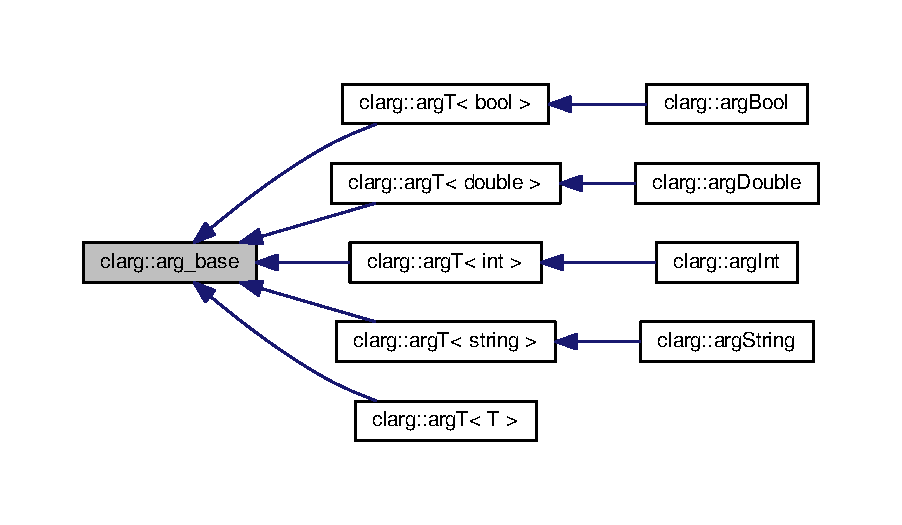
\includegraphics[width=350pt]{classclarg_1_1arg__base__inherit__graph}
\end{center}
\end{figure}
\subsection*{Public Member Functions}
\begin{DoxyCompactItemize}
\item 
{\bfseries arg\+\_\+base} (const char $\ast$name, const char $\ast$desc)\hypertarget{classclarg_1_1arg__base_a7a37ba86e5e5e73b86af0e91e704bc4d}{}\label{classclarg_1_1arg__base_a7a37ba86e5e5e73b86af0e91e704bc4d}

\item 
const string \& {\bfseries get\+\_\+name} () const \hypertarget{classclarg_1_1arg__base_a021c1fabeb75a62b7babb578b5e7d187}{}\label{classclarg_1_1arg__base_a021c1fabeb75a62b7babb578b5e7d187}

\item 
const string \& {\bfseries get\+\_\+desc} () const \hypertarget{classclarg_1_1arg__base_a4a2513e871d1fa654838bc9fe47f84b7}{}\label{classclarg_1_1arg__base_a4a2513e871d1fa654838bc9fe47f84b7}

\item 
bool {\bfseries was\+\_\+set} () const \hypertarget{classclarg_1_1arg__base_aa92067620e266422f44243c7b247782f}{}\label{classclarg_1_1arg__base_aa92067620e266422f44243c7b247782f}

\item 
void {\bfseries mark\+\_\+set} (bool m)\hypertarget{classclarg_1_1arg__base_a339f03baa455901e1eed0708da3e8ce4}{}\label{classclarg_1_1arg__base_a339f03baa455901e1eed0708da3e8ce4}

\end{DoxyCompactItemize}
\subsection*{Protected Member Functions}
\begin{DoxyCompactItemize}
\item 
virtual int \hyperlink{classclarg_1_1arg__base_a4c0e6afc44de0d825334a41d4ef5b813}{parse\+\_\+parameters} (int argc, char $\ast$argv\mbox{[}$\,$\mbox{]})=0
\item 
virtual void \hyperlink{classclarg_1_1arg__base_a476be3712ecd028fee248cef14cc3cfb}{write\+\_\+parameters} (ostream \&os, bool def=false) const =0
\end{DoxyCompactItemize}
\subsection*{Protected Attributes}
\begin{DoxyCompactItemize}
\item 
bool \hyperlink{classclarg_1_1arg__base_a897ba15feb1390687d072acae6c69512}{arg\+\_\+set}
\item 
string \hyperlink{classclarg_1_1arg__base_af0e1e1240bd9779d84d2b4d9f078f9e2}{arg\+\_\+name}
\item 
string \hyperlink{classclarg_1_1arg__base_adef436501e6af061da6e3b0652e43704}{arg\+\_\+desc}
\end{DoxyCompactItemize}
\subsection*{Friends}
\begin{DoxyCompactItemize}
\item 
class {\bfseries args\+\_\+container}\hypertarget{classclarg_1_1arg__base_a43417d1ca2f28ea0936749ee5fc8fab0}{}\label{classclarg_1_1arg__base_a43417d1ca2f28ea0936749ee5fc8fab0}

\end{DoxyCompactItemize}


\subsection{Detailed Description}
The base argument class. Manages arguments names and descriptions. 

\subsection{Member Function Documentation}
\index{clarg\+::arg\+\_\+base@{clarg\+::arg\+\_\+base}!parse\+\_\+parameters@{parse\+\_\+parameters}}
\index{parse\+\_\+parameters@{parse\+\_\+parameters}!clarg\+::arg\+\_\+base@{clarg\+::arg\+\_\+base}}
\subsubsection[{\texorpdfstring{parse\+\_\+parameters(int argc, char $\ast$argv[])=0}{parse_parameters(int argc, char *argv[])=0}}]{\setlength{\rightskip}{0pt plus 5cm}virtual int clarg\+::arg\+\_\+base\+::parse\+\_\+parameters (
\begin{DoxyParamCaption}
\item[{int}]{argc, }
\item[{char $\ast$}]{argv\mbox{[}$\,$\mbox{]}}
\end{DoxyParamCaption}
)\hspace{0.3cm}{\ttfamily [protected]}, {\ttfamily [pure virtual]}}\hypertarget{classclarg_1_1arg__base_a4c0e6afc44de0d825334a41d4ef5b813}{}\label{classclarg_1_1arg__base_a4c0e6afc44de0d825334a41d4ef5b813}
Parse the argument parameters. Must be implemented by the specialized argument class. When parsing, make sure you copy the parsed parameters into the arg\+\_\+parameters array. Returns the number of parameters parsed if ok, -\/1 if an error occured. 

Implemented in \hyperlink{classclarg_1_1arg_bool_a4e75d91370d7a99c8ec56eee6e112eef}{clarg\+::arg\+Bool}, \hyperlink{classclarg_1_1arg_double_abdf04919fbed93b3255256a9e1e4faca}{clarg\+::arg\+Double}, \hyperlink{classclarg_1_1arg_int_aa65ff016fe6834afd79663c939dc2864}{clarg\+::arg\+Int}, and \hyperlink{classclarg_1_1arg_string_a06a724f38fc4df3732d9ab2072705c6c}{clarg\+::arg\+String}.

\index{clarg\+::arg\+\_\+base@{clarg\+::arg\+\_\+base}!write\+\_\+parameters@{write\+\_\+parameters}}
\index{write\+\_\+parameters@{write\+\_\+parameters}!clarg\+::arg\+\_\+base@{clarg\+::arg\+\_\+base}}
\subsubsection[{\texorpdfstring{write\+\_\+parameters(ostream \&os, bool def=false) const =0}{write_parameters(ostream &os, bool def=false) const =0}}]{\setlength{\rightskip}{0pt plus 5cm}virtual void clarg\+::arg\+\_\+base\+::write\+\_\+parameters (
\begin{DoxyParamCaption}
\item[{ostream \&}]{os, }
\item[{bool}]{def = {\ttfamily false}}
\end{DoxyParamCaption}
) const\hspace{0.3cm}{\ttfamily [protected]}, {\ttfamily [pure virtual]}}\hypertarget{classclarg_1_1arg__base_a476be3712ecd028fee248cef14cc3cfb}{}\label{classclarg_1_1arg__base_a476be3712ecd028fee248cef14cc3cfb}
write the argument parameters into the output stream. 

Implemented in \hyperlink{classclarg_1_1arg_bool_ae254f2a52551c3c811ad08c248d6b4a9}{clarg\+::arg\+Bool}, \hyperlink{classclarg_1_1arg_double_ad4968ff300091cc01022836310ee2383}{clarg\+::arg\+Double}, \hyperlink{classclarg_1_1arg_int_a907539c5963530661a3df01735d39f37}{clarg\+::arg\+Int}, and \hyperlink{classclarg_1_1arg_string_ae336afebabd08c78b5323e1c6eba8ba7}{clarg\+::arg\+String}.



\subsection{Member Data Documentation}
\index{clarg\+::arg\+\_\+base@{clarg\+::arg\+\_\+base}!arg\+\_\+desc@{arg\+\_\+desc}}
\index{arg\+\_\+desc@{arg\+\_\+desc}!clarg\+::arg\+\_\+base@{clarg\+::arg\+\_\+base}}
\subsubsection[{\texorpdfstring{arg\+\_\+desc}{arg_desc}}]{\setlength{\rightskip}{0pt plus 5cm}string clarg\+::arg\+\_\+base\+::arg\+\_\+desc\hspace{0.3cm}{\ttfamily [protected]}}\hypertarget{classclarg_1_1arg__base_adef436501e6af061da6e3b0652e43704}{}\label{classclarg_1_1arg__base_adef436501e6af061da6e3b0652e43704}
The argument description. \index{clarg\+::arg\+\_\+base@{clarg\+::arg\+\_\+base}!arg\+\_\+name@{arg\+\_\+name}}
\index{arg\+\_\+name@{arg\+\_\+name}!clarg\+::arg\+\_\+base@{clarg\+::arg\+\_\+base}}
\subsubsection[{\texorpdfstring{arg\+\_\+name}{arg_name}}]{\setlength{\rightskip}{0pt plus 5cm}string clarg\+::arg\+\_\+base\+::arg\+\_\+name\hspace{0.3cm}{\ttfamily [protected]}}\hypertarget{classclarg_1_1arg__base_af0e1e1240bd9779d84d2b4d9f078f9e2}{}\label{classclarg_1_1arg__base_af0e1e1240bd9779d84d2b4d9f078f9e2}
The argument name. \index{clarg\+::arg\+\_\+base@{clarg\+::arg\+\_\+base}!arg\+\_\+set@{arg\+\_\+set}}
\index{arg\+\_\+set@{arg\+\_\+set}!clarg\+::arg\+\_\+base@{clarg\+::arg\+\_\+base}}
\subsubsection[{\texorpdfstring{arg\+\_\+set}{arg_set}}]{\setlength{\rightskip}{0pt plus 5cm}bool clarg\+::arg\+\_\+base\+::arg\+\_\+set\hspace{0.3cm}{\ttfamily [protected]}}\hypertarget{classclarg_1_1arg__base_a897ba15feb1390687d072acae6c69512}{}\label{classclarg_1_1arg__base_a897ba15feb1390687d072acae6c69512}
True if the argument was set 

The documentation for this class was generated from the following files\+:\begin{DoxyCompactItemize}
\item 
include/arglib/arglib.\+hpp\item 
arglib/arglib.\+cpp\end{DoxyCompactItemize}

\hypertarget{classclarg_1_1arg_bool}{}\section{clarg\+:\+:arg\+Bool Class Reference}
\label{classclarg_1_1arg_bool}\index{clarg\+::arg\+Bool@{clarg\+::arg\+Bool}}


{\ttfamily \#include $<$arglib.\+hpp$>$}



Inheritance diagram for clarg\+:\+:arg\+Bool\+:\nopagebreak
\begin{figure}[H]
\begin{center}
\leavevmode
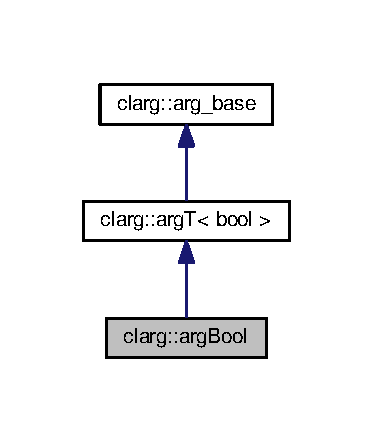
\includegraphics[width=179pt]{classclarg_1_1arg_bool__inherit__graph}
\end{center}
\end{figure}


Collaboration diagram for clarg\+:\+:arg\+Bool\+:\nopagebreak
\begin{figure}[H]
\begin{center}
\leavevmode
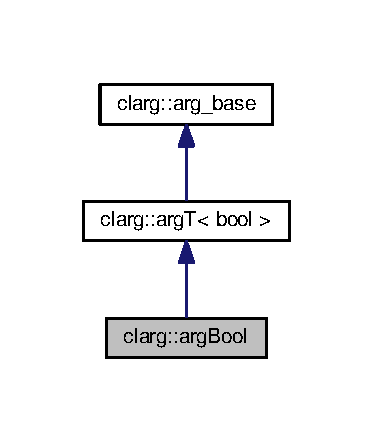
\includegraphics[width=179pt]{classclarg_1_1arg_bool__coll__graph}
\end{center}
\end{figure}
\subsection*{Public Member Functions}
\begin{DoxyCompactItemize}
\item 
{\bfseries arg\+Bool} (const char $\ast$arg, const char $\ast$desc, bool v=false)\hypertarget{classclarg_1_1arg_bool_a9fcf0dd302882e22d36ee41547ad04ec}{}\label{classclarg_1_1arg_bool_a9fcf0dd302882e22d36ee41547ad04ec}

\end{DoxyCompactItemize}
\subsection*{Protected Member Functions}
\begin{DoxyCompactItemize}
\item 
int \hyperlink{classclarg_1_1arg_bool_a4e75d91370d7a99c8ec56eee6e112eef}{parse\+\_\+parameters} (int, char $\ast$\mbox{[}$\,$\mbox{]})
\item 
void \hyperlink{classclarg_1_1arg_bool_ae254f2a52551c3c811ad08c248d6b4a9}{write\+\_\+parameters} (ostream \&, bool) const 
\end{DoxyCompactItemize}
\subsection*{Additional Inherited Members}


\subsection{Detailed Description}
Boolean argument class. 

\subsection{Member Function Documentation}
\index{clarg\+::arg\+Bool@{clarg\+::arg\+Bool}!parse\+\_\+parameters@{parse\+\_\+parameters}}
\index{parse\+\_\+parameters@{parse\+\_\+parameters}!clarg\+::arg\+Bool@{clarg\+::arg\+Bool}}
\subsubsection[{\texorpdfstring{parse\+\_\+parameters(int, char $\ast$[])}{parse_parameters(int, char *[])}}]{\setlength{\rightskip}{0pt plus 5cm}int clarg\+::arg\+Bool\+::parse\+\_\+parameters (
\begin{DoxyParamCaption}
\item[{int}]{argc, }
\item[{char $\ast$}]{argv\mbox{[}$\,$\mbox{]}}
\end{DoxyParamCaption}
)\hspace{0.3cm}{\ttfamily [inline]}, {\ttfamily [protected]}, {\ttfamily [virtual]}}\hypertarget{classclarg_1_1arg_bool_a4e75d91370d7a99c8ec56eee6e112eef}{}\label{classclarg_1_1arg_bool_a4e75d91370d7a99c8ec56eee6e112eef}
Parse the argument parameters. Must be implemented by the specialized argument class. When parsing, make sure you copy the parsed parameters into the arg\+\_\+parameters array. Returns the number of parameters parsed if ok, -\/1 if an error occured. 

Implements \hyperlink{classclarg_1_1arg__base_a4c0e6afc44de0d825334a41d4ef5b813}{clarg\+::arg\+\_\+base}.

\index{clarg\+::arg\+Bool@{clarg\+::arg\+Bool}!write\+\_\+parameters@{write\+\_\+parameters}}
\index{write\+\_\+parameters@{write\+\_\+parameters}!clarg\+::arg\+Bool@{clarg\+::arg\+Bool}}
\subsubsection[{\texorpdfstring{write\+\_\+parameters(ostream \&, bool) const }{write_parameters(ostream &, bool) const }}]{\setlength{\rightskip}{0pt plus 5cm}void clarg\+::arg\+Bool\+::write\+\_\+parameters (
\begin{DoxyParamCaption}
\item[{ostream \&}]{os, }
\item[{bool}]{def}
\end{DoxyParamCaption}
) const\hspace{0.3cm}{\ttfamily [inline]}, {\ttfamily [protected]}, {\ttfamily [virtual]}}\hypertarget{classclarg_1_1arg_bool_ae254f2a52551c3c811ad08c248d6b4a9}{}\label{classclarg_1_1arg_bool_ae254f2a52551c3c811ad08c248d6b4a9}
write the argument parameters into the output stream. 

Implements \hyperlink{classclarg_1_1arg__base_a476be3712ecd028fee248cef14cc3cfb}{clarg\+::arg\+\_\+base}.



The documentation for this class was generated from the following file\+:\begin{DoxyCompactItemize}
\item 
include/arglib/arglib.\+hpp\end{DoxyCompactItemize}

\hypertarget{classclarg_1_1arg_double}{}\section{clarg\+:\+:arg\+Double Class Reference}
\label{classclarg_1_1arg_double}\index{clarg\+::arg\+Double@{clarg\+::arg\+Double}}


{\ttfamily \#include $<$arglib.\+hpp$>$}



Inheritance diagram for clarg\+:\+:arg\+Double\+:\nopagebreak
\begin{figure}[H]
\begin{center}
\leavevmode
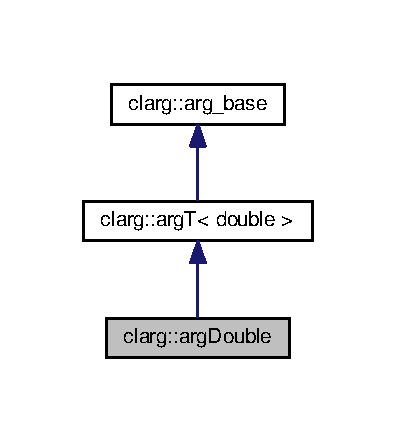
\includegraphics[width=190pt]{classclarg_1_1arg_double__inherit__graph}
\end{center}
\end{figure}


Collaboration diagram for clarg\+:\+:arg\+Double\+:\nopagebreak
\begin{figure}[H]
\begin{center}
\leavevmode
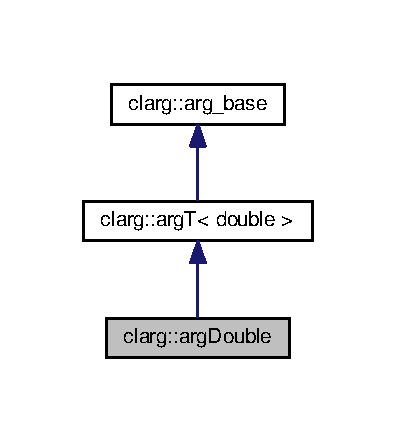
\includegraphics[width=190pt]{classclarg_1_1arg_double__coll__graph}
\end{center}
\end{figure}
\subsection*{Public Member Functions}
\begin{DoxyCompactItemize}
\item 
{\bfseries arg\+Double} (const char $\ast$arg, const char $\ast$desc, double v=0.\+0)\hypertarget{classclarg_1_1arg_double_adc69c6c39b2490368e6d93445275714e}{}\label{classclarg_1_1arg_double_adc69c6c39b2490368e6d93445275714e}

\end{DoxyCompactItemize}
\subsection*{Protected Member Functions}
\begin{DoxyCompactItemize}
\item 
int \hyperlink{classclarg_1_1arg_double_abdf04919fbed93b3255256a9e1e4faca}{parse\+\_\+parameters} (int argc, char $\ast$argv\mbox{[}$\,$\mbox{]})
\item 
void \hyperlink{classclarg_1_1arg_double_ad4968ff300091cc01022836310ee2383}{write\+\_\+parameters} (ostream \&os, bool def) const 
\end{DoxyCompactItemize}
\subsection*{Additional Inherited Members}


\subsection{Detailed Description}
Double argument class. 

\subsection{Member Function Documentation}
\index{clarg\+::arg\+Double@{clarg\+::arg\+Double}!parse\+\_\+parameters@{parse\+\_\+parameters}}
\index{parse\+\_\+parameters@{parse\+\_\+parameters}!clarg\+::arg\+Double@{clarg\+::arg\+Double}}
\subsubsection[{\texorpdfstring{parse\+\_\+parameters(int argc, char $\ast$argv[])}{parse_parameters(int argc, char *argv[])}}]{\setlength{\rightskip}{0pt plus 5cm}int clarg\+::arg\+Double\+::parse\+\_\+parameters (
\begin{DoxyParamCaption}
\item[{int}]{argc, }
\item[{char $\ast$}]{argv\mbox{[}$\,$\mbox{]}}
\end{DoxyParamCaption}
)\hspace{0.3cm}{\ttfamily [inline]}, {\ttfamily [protected]}, {\ttfamily [virtual]}}\hypertarget{classclarg_1_1arg_double_abdf04919fbed93b3255256a9e1e4faca}{}\label{classclarg_1_1arg_double_abdf04919fbed93b3255256a9e1e4faca}
Parse the argument parameters. Must be implemented by the specialized argument class. When parsing, make sure you copy the parsed parameters into the arg\+\_\+parameters array. Returns the number of parameters parsed if ok, -\/1 if an error occured. 

Implements \hyperlink{classclarg_1_1arg__base_a4c0e6afc44de0d825334a41d4ef5b813}{clarg\+::arg\+\_\+base}.

\index{clarg\+::arg\+Double@{clarg\+::arg\+Double}!write\+\_\+parameters@{write\+\_\+parameters}}
\index{write\+\_\+parameters@{write\+\_\+parameters}!clarg\+::arg\+Double@{clarg\+::arg\+Double}}
\subsubsection[{\texorpdfstring{write\+\_\+parameters(ostream \&os, bool def) const }{write_parameters(ostream &os, bool def) const }}]{\setlength{\rightskip}{0pt plus 5cm}void clarg\+::arg\+Double\+::write\+\_\+parameters (
\begin{DoxyParamCaption}
\item[{ostream \&}]{os, }
\item[{bool}]{def}
\end{DoxyParamCaption}
) const\hspace{0.3cm}{\ttfamily [inline]}, {\ttfamily [protected]}, {\ttfamily [virtual]}}\hypertarget{classclarg_1_1arg_double_ad4968ff300091cc01022836310ee2383}{}\label{classclarg_1_1arg_double_ad4968ff300091cc01022836310ee2383}
write the argument parameters into the output stream. 

Implements \hyperlink{classclarg_1_1arg__base_a476be3712ecd028fee248cef14cc3cfb}{clarg\+::arg\+\_\+base}.



The documentation for this class was generated from the following file\+:\begin{DoxyCompactItemize}
\item 
include/arglib/arglib.\+hpp\end{DoxyCompactItemize}

\hypertarget{classclarg_1_1arg_int}{}\section{clarg\+:\+:arg\+Int Class Reference}
\label{classclarg_1_1arg_int}\index{clarg\+::arg\+Int@{clarg\+::arg\+Int}}


{\ttfamily \#include $<$arglib.\+hpp$>$}



Inheritance diagram for clarg\+:\+:arg\+Int\+:\nopagebreak
\begin{figure}[H]
\begin{center}
\leavevmode
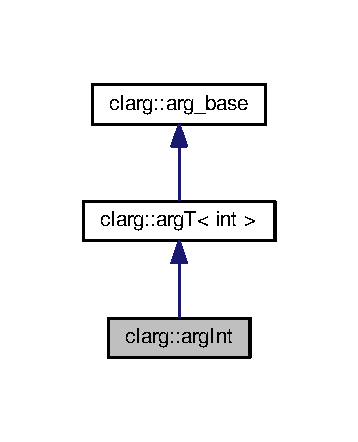
\includegraphics[width=172pt]{classclarg_1_1arg_int__inherit__graph}
\end{center}
\end{figure}


Collaboration diagram for clarg\+:\+:arg\+Int\+:\nopagebreak
\begin{figure}[H]
\begin{center}
\leavevmode
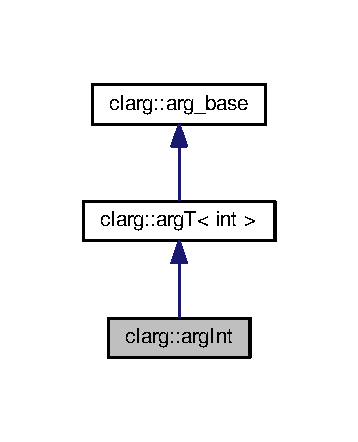
\includegraphics[width=172pt]{classclarg_1_1arg_int__coll__graph}
\end{center}
\end{figure}
\subsection*{Public Member Functions}
\begin{DoxyCompactItemize}
\item 
{\bfseries arg\+Int} (const char $\ast$arg, const char $\ast$desc, int v=0)\hypertarget{classclarg_1_1arg_int_aac929eff64f26e154973b504cb085952}{}\label{classclarg_1_1arg_int_aac929eff64f26e154973b504cb085952}

\end{DoxyCompactItemize}
\subsection*{Protected Member Functions}
\begin{DoxyCompactItemize}
\item 
int \hyperlink{classclarg_1_1arg_int_aa65ff016fe6834afd79663c939dc2864}{parse\+\_\+parameters} (int argc, char $\ast$argv\mbox{[}$\,$\mbox{]})
\item 
void \hyperlink{classclarg_1_1arg_int_a907539c5963530661a3df01735d39f37}{write\+\_\+parameters} (ostream \&os, bool def) const 
\end{DoxyCompactItemize}
\subsection*{Additional Inherited Members}


\subsection{Detailed Description}
Integer argument class. 

\subsection{Member Function Documentation}
\index{clarg\+::arg\+Int@{clarg\+::arg\+Int}!parse\+\_\+parameters@{parse\+\_\+parameters}}
\index{parse\+\_\+parameters@{parse\+\_\+parameters}!clarg\+::arg\+Int@{clarg\+::arg\+Int}}
\subsubsection[{\texorpdfstring{parse\+\_\+parameters(int argc, char $\ast$argv[])}{parse_parameters(int argc, char *argv[])}}]{\setlength{\rightskip}{0pt plus 5cm}int clarg\+::arg\+Int\+::parse\+\_\+parameters (
\begin{DoxyParamCaption}
\item[{int}]{argc, }
\item[{char $\ast$}]{argv\mbox{[}$\,$\mbox{]}}
\end{DoxyParamCaption}
)\hspace{0.3cm}{\ttfamily [inline]}, {\ttfamily [protected]}, {\ttfamily [virtual]}}\hypertarget{classclarg_1_1arg_int_aa65ff016fe6834afd79663c939dc2864}{}\label{classclarg_1_1arg_int_aa65ff016fe6834afd79663c939dc2864}
Parse the argument parameters. Must be implemented by the specialized argument class. When parsing, make sure you copy the parsed parameters into the arg\+\_\+parameters array. Returns the number of parameters parsed if ok, -\/1 if an error occured. 

Implements \hyperlink{classclarg_1_1arg__base_a4c0e6afc44de0d825334a41d4ef5b813}{clarg\+::arg\+\_\+base}.

\index{clarg\+::arg\+Int@{clarg\+::arg\+Int}!write\+\_\+parameters@{write\+\_\+parameters}}
\index{write\+\_\+parameters@{write\+\_\+parameters}!clarg\+::arg\+Int@{clarg\+::arg\+Int}}
\subsubsection[{\texorpdfstring{write\+\_\+parameters(ostream \&os, bool def) const }{write_parameters(ostream &os, bool def) const }}]{\setlength{\rightskip}{0pt plus 5cm}void clarg\+::arg\+Int\+::write\+\_\+parameters (
\begin{DoxyParamCaption}
\item[{ostream \&}]{os, }
\item[{bool}]{def}
\end{DoxyParamCaption}
) const\hspace{0.3cm}{\ttfamily [inline]}, {\ttfamily [protected]}, {\ttfamily [virtual]}}\hypertarget{classclarg_1_1arg_int_a907539c5963530661a3df01735d39f37}{}\label{classclarg_1_1arg_int_a907539c5963530661a3df01735d39f37}
write the argument parameters into the output stream. 

Implements \hyperlink{classclarg_1_1arg__base_a476be3712ecd028fee248cef14cc3cfb}{clarg\+::arg\+\_\+base}.



The documentation for this class was generated from the following file\+:\begin{DoxyCompactItemize}
\item 
include/arglib/arglib.\+hpp\end{DoxyCompactItemize}

\hypertarget{classclarg_1_1args__container}{}\section{clarg\+:\+:args\+\_\+container Class Reference}
\label{classclarg_1_1args__container}\index{clarg\+::args\+\_\+container@{clarg\+::args\+\_\+container}}
\subsection*{Public Member Functions}
\begin{DoxyCompactItemize}
\item 
void {\bfseries register\+\_\+argument} (\hyperlink{classclarg_1_1arg__base}{arg\+\_\+base} $\ast$arg)\hypertarget{classclarg_1_1args__container_a24df956afe76b8f3377dbf622bcad957}{}\label{classclarg_1_1args__container_a24df956afe76b8f3377dbf622bcad957}

\item 
void {\bfseries arguments\+\_\+descriptions} (ostream \&os, string prefix, string suffix)\hypertarget{classclarg_1_1args__container_a0f081963267f4b66924633e29255dc3d}{}\label{classclarg_1_1args__container_a0f081963267f4b66924633e29255dc3d}

\item 
void {\bfseries list\+\_\+arguments} (ostream \&os, bool defined\+\_\+only)\hypertarget{classclarg_1_1args__container_ae2f55011dcec5e394b4fc7b5ce18ef4a}{}\label{classclarg_1_1args__container_ae2f55011dcec5e394b4fc7b5ce18ef4a}

\item 
int \hyperlink{classclarg_1_1args__container_a0d6feb51358dec2f5ba941ed837d1c1a}{parse\+\_\+arguments\+\_\+from\+\_\+file} ()
\item 
int {\bfseries parse\+\_\+arguments} (int argc, char $\ast$argv\mbox{[}$\,$\mbox{]})\hypertarget{classclarg_1_1args__container_a9bc7411d20a2b8fcfc0f720ddd8d401a}{}\label{classclarg_1_1args__container_a9bc7411d20a2b8fcfc0f720ddd8d401a}

\end{DoxyCompactItemize}
\subsection*{Public Attributes}
\begin{DoxyCompactItemize}
\item 
M\+AP$<$ string, \hyperlink{classclarg_1_1arg__base}{arg\+\_\+base} $\ast$ $>$ {\bfseries args}\hypertarget{classclarg_1_1args__container_ad194851fa063d34987575e0ee13d1c87}{}\label{classclarg_1_1args__container_ad194851fa063d34987575e0ee13d1c87}

\item 
string {\bfseries prog\+\_\+name}\hypertarget{classclarg_1_1args__container_a98f0ec6ac0e5fb595c6e0ec04a9770c8}{}\label{classclarg_1_1args__container_a98f0ec6ac0e5fb595c6e0ec04a9770c8}

\end{DoxyCompactItemize}


\subsection{Detailed Description}
Arguments container. All the arguments are added into this object. 

\subsection{Member Function Documentation}
\index{clarg\+::args\+\_\+container@{clarg\+::args\+\_\+container}!parse\+\_\+arguments\+\_\+from\+\_\+file@{parse\+\_\+arguments\+\_\+from\+\_\+file}}
\index{parse\+\_\+arguments\+\_\+from\+\_\+file@{parse\+\_\+arguments\+\_\+from\+\_\+file}!clarg\+::args\+\_\+container@{clarg\+::args\+\_\+container}}
\subsubsection[{\texorpdfstring{parse\+\_\+arguments\+\_\+from\+\_\+file()}{parse_arguments_from_file()}}]{\setlength{\rightskip}{0pt plus 5cm}int clarg\+::args\+\_\+container\+::parse\+\_\+arguments\+\_\+from\+\_\+file (
\begin{DoxyParamCaption}
{}
\end{DoxyParamCaption}
)\hspace{0.3cm}{\ttfamily [inline]}}\hypertarget{classclarg_1_1args__container_a0d6feb51358dec2f5ba941ed837d1c1a}{}\label{classclarg_1_1args__container_a0d6feb51358dec2f5ba941ed837d1c1a}
Read the arguments from file. Returns 0 if ok, != 0 otherwise. T\+O\+DO\+: this is not implemented yet. The goal of this method is to parser all the arguments from an argument file. In this way, you may dump all the arguments used in a given run and re-\/use them by parsing from the file. To do so, you may infoke this method. 

The documentation for this class was generated from the following file\+:\begin{DoxyCompactItemize}
\item 
arglib/arglib.\+cpp\end{DoxyCompactItemize}

\hypertarget{classclarg_1_1arg_string}{}\section{clarg\+:\+:arg\+String Class Reference}
\label{classclarg_1_1arg_string}\index{clarg\+::arg\+String@{clarg\+::arg\+String}}


{\ttfamily \#include $<$arglib.\+hpp$>$}



Inheritance diagram for clarg\+:\+:arg\+String\+:\nopagebreak
\begin{figure}[H]
\begin{center}
\leavevmode
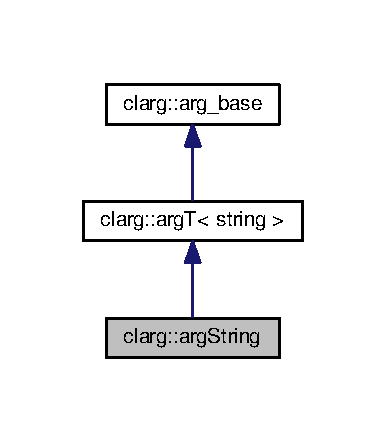
\includegraphics[width=185pt]{classclarg_1_1arg_string__inherit__graph}
\end{center}
\end{figure}


Collaboration diagram for clarg\+:\+:arg\+String\+:\nopagebreak
\begin{figure}[H]
\begin{center}
\leavevmode
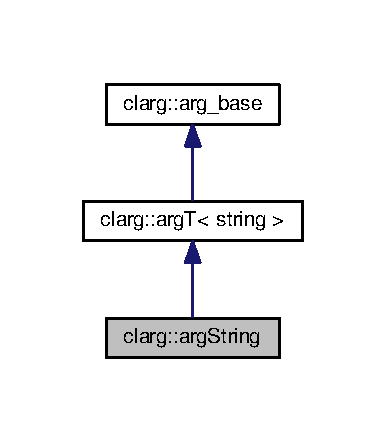
\includegraphics[width=185pt]{classclarg_1_1arg_string__coll__graph}
\end{center}
\end{figure}
\subsection*{Public Member Functions}
\begin{DoxyCompactItemize}
\item 
{\bfseries arg\+String} (const char $\ast$arg, const char $\ast$desc, string v)\hypertarget{classclarg_1_1arg_string_a8b6bad644226b839a2ec02c6c8c03eec}{}\label{classclarg_1_1arg_string_a8b6bad644226b839a2ec02c6c8c03eec}

\end{DoxyCompactItemize}
\subsection*{Protected Member Functions}
\begin{DoxyCompactItemize}
\item 
int \hyperlink{classclarg_1_1arg_string_a06a724f38fc4df3732d9ab2072705c6c}{parse\+\_\+parameters} (int argc, char $\ast$argv\mbox{[}$\,$\mbox{]})
\item 
void \hyperlink{classclarg_1_1arg_string_ae336afebabd08c78b5323e1c6eba8ba7}{write\+\_\+parameters} (ostream \&os, bool def) const 
\end{DoxyCompactItemize}
\subsection*{Additional Inherited Members}


\subsection{Detailed Description}
String argument class. 

\subsection{Member Function Documentation}
\index{clarg\+::arg\+String@{clarg\+::arg\+String}!parse\+\_\+parameters@{parse\+\_\+parameters}}
\index{parse\+\_\+parameters@{parse\+\_\+parameters}!clarg\+::arg\+String@{clarg\+::arg\+String}}
\subsubsection[{\texorpdfstring{parse\+\_\+parameters(int argc, char $\ast$argv[])}{parse_parameters(int argc, char *argv[])}}]{\setlength{\rightskip}{0pt plus 5cm}int clarg\+::arg\+String\+::parse\+\_\+parameters (
\begin{DoxyParamCaption}
\item[{int}]{argc, }
\item[{char $\ast$}]{argv\mbox{[}$\,$\mbox{]}}
\end{DoxyParamCaption}
)\hspace{0.3cm}{\ttfamily [inline]}, {\ttfamily [protected]}, {\ttfamily [virtual]}}\hypertarget{classclarg_1_1arg_string_a06a724f38fc4df3732d9ab2072705c6c}{}\label{classclarg_1_1arg_string_a06a724f38fc4df3732d9ab2072705c6c}
Parse the argument parameters. Must be implemented by the specialized argument class. When parsing, make sure you copy the parsed parameters into the arg\+\_\+parameters array. Returns the number of parameters parsed if ok, -\/1 if an error occured. 

Implements \hyperlink{classclarg_1_1arg__base_a4c0e6afc44de0d825334a41d4ef5b813}{clarg\+::arg\+\_\+base}.

\index{clarg\+::arg\+String@{clarg\+::arg\+String}!write\+\_\+parameters@{write\+\_\+parameters}}
\index{write\+\_\+parameters@{write\+\_\+parameters}!clarg\+::arg\+String@{clarg\+::arg\+String}}
\subsubsection[{\texorpdfstring{write\+\_\+parameters(ostream \&os, bool def) const }{write_parameters(ostream &os, bool def) const }}]{\setlength{\rightskip}{0pt plus 5cm}void clarg\+::arg\+String\+::write\+\_\+parameters (
\begin{DoxyParamCaption}
\item[{ostream \&}]{os, }
\item[{bool}]{def}
\end{DoxyParamCaption}
) const\hspace{0.3cm}{\ttfamily [inline]}, {\ttfamily [protected]}, {\ttfamily [virtual]}}\hypertarget{classclarg_1_1arg_string_ae336afebabd08c78b5323e1c6eba8ba7}{}\label{classclarg_1_1arg_string_ae336afebabd08c78b5323e1c6eba8ba7}
write the argument parameters into the output stream. 

Implements \hyperlink{classclarg_1_1arg__base_a476be3712ecd028fee248cef14cc3cfb}{clarg\+::arg\+\_\+base}.



The documentation for this class was generated from the following file\+:\begin{DoxyCompactItemize}
\item 
include/arglib/arglib.\+hpp\end{DoxyCompactItemize}

\hypertarget{classclarg_1_1arg_t}{}\section{clarg\+:\+:argT$<$ T $>$ Class Template Reference}
\label{classclarg_1_1arg_t}\index{clarg\+::arg\+T$<$ T $>$@{clarg\+::arg\+T$<$ T $>$}}


{\ttfamily \#include $<$arglib.\+hpp$>$}



Inheritance diagram for clarg\+:\+:argT$<$ T $>$\+:\nopagebreak
\begin{figure}[H]
\begin{center}
\leavevmode
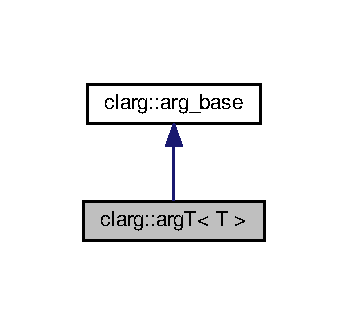
\includegraphics[width=167pt]{classclarg_1_1arg_t__inherit__graph}
\end{center}
\end{figure}


Collaboration diagram for clarg\+:\+:argT$<$ T $>$\+:\nopagebreak
\begin{figure}[H]
\begin{center}
\leavevmode
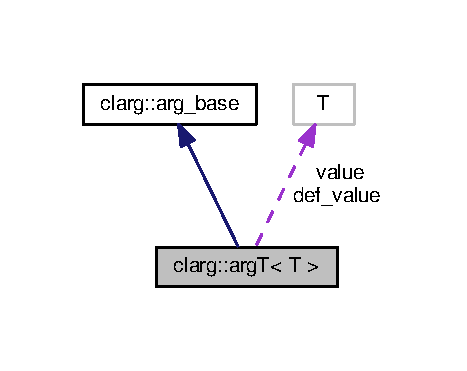
\includegraphics[width=224pt]{classclarg_1_1arg_t__coll__graph}
\end{center}
\end{figure}
\subsection*{Public Member Functions}
\begin{DoxyCompactItemize}
\item 
{\bfseries argT} (const char $\ast$arg, const char $\ast$desc)\hypertarget{classclarg_1_1arg_t_a944077071cc380e8abd089e40ad10ee9}{}\label{classclarg_1_1arg_t_a944077071cc380e8abd089e40ad10ee9}

\item 
const T \& {\bfseries get\+\_\+value} () const \hypertarget{classclarg_1_1arg_t_ac7a7862cc0598d26b61d1756e4d33c34}{}\label{classclarg_1_1arg_t_ac7a7862cc0598d26b61d1756e4d33c34}

\item 
void {\bfseries set\+\_\+value} (const T \&v) const \hypertarget{classclarg_1_1arg_t_a3d752cdf63502e421c1675c538be1fbb}{}\label{classclarg_1_1arg_t_a3d752cdf63502e421c1675c538be1fbb}

\end{DoxyCompactItemize}
\subsection*{Protected Attributes}
\begin{DoxyCompactItemize}
\item 
T {\bfseries value}\hypertarget{classclarg_1_1arg_t_a98a6007ac097eb86d5593f9bb57f28e5}{}\label{classclarg_1_1arg_t_a98a6007ac097eb86d5593f9bb57f28e5}

\item 
T {\bfseries def\+\_\+value}\hypertarget{classclarg_1_1arg_t_abc32c1e94eb88b45a5dfa45aaf7ba988}{}\label{classclarg_1_1arg_t_abc32c1e94eb88b45a5dfa45aaf7ba988}

\end{DoxyCompactItemize}
\subsection*{Additional Inherited Members}


\subsection{Detailed Description}
\subsubsection*{template$<$class T$>$\\*
class clarg\+::arg\+T$<$ T $>$}

The argument template class. 

The documentation for this class was generated from the following file\+:\begin{DoxyCompactItemize}
\item 
include/arglib/arglib.\+hpp\end{DoxyCompactItemize}

\hypertarget{structspp___1_1_combiner}{}\section{spp\+\_\+\+:\+:Combiner$<$ T, sz $>$ Struct Template Reference}
\label{structspp___1_1_combiner}\index{spp\+\_\+\+::\+Combiner$<$ T, sz $>$@{spp\+\_\+\+::\+Combiner$<$ T, sz $>$}}
\subsection*{Public Member Functions}
\begin{DoxyCompactItemize}
\item 
void {\bfseries operator()} (T \&seed, T value)\hypertarget{structspp___1_1_combiner_ac1b48a245f1e5a2ceea3dee737062f5d}{}\label{structspp___1_1_combiner_ac1b48a245f1e5a2ceea3dee737062f5d}

\end{DoxyCompactItemize}


The documentation for this struct was generated from the following file\+:\begin{DoxyCompactItemize}
\item 
include/sparsepp/spp\+\_\+utils.\+h\end{DoxyCompactItemize}

\hypertarget{structspp___1_1_combiner_3_01_t_00_014_01_4}{}\section{spp\+\_\+\+:\+:Combiner$<$ T, 4 $>$ Struct Template Reference}
\label{structspp___1_1_combiner_3_01_t_00_014_01_4}\index{spp\+\_\+\+::\+Combiner$<$ T, 4 $>$@{spp\+\_\+\+::\+Combiner$<$ T, 4 $>$}}
\subsection*{Public Member Functions}
\begin{DoxyCompactItemize}
\item 
void {\bfseries operator()} (T \&seed, T value)\hypertarget{structspp___1_1_combiner_3_01_t_00_014_01_4_aeacf87124749fd2f7269e8e04dcb410a}{}\label{structspp___1_1_combiner_3_01_t_00_014_01_4_aeacf87124749fd2f7269e8e04dcb410a}

\end{DoxyCompactItemize}


The documentation for this struct was generated from the following file\+:\begin{DoxyCompactItemize}
\item 
include/sparsepp/spp\+\_\+utils.\+h\end{DoxyCompactItemize}

\hypertarget{structspp___1_1_combiner_3_01_t_00_018_01_4}{}\section{spp\+\_\+\+:\+:Combiner$<$ T, 8 $>$ Struct Template Reference}
\label{structspp___1_1_combiner_3_01_t_00_018_01_4}\index{spp\+\_\+\+::\+Combiner$<$ T, 8 $>$@{spp\+\_\+\+::\+Combiner$<$ T, 8 $>$}}
\subsection*{Public Member Functions}
\begin{DoxyCompactItemize}
\item 
void {\bfseries operator()} (T \&seed, T value)\hypertarget{structspp___1_1_combiner_3_01_t_00_018_01_4_af33f6513ca59344517b87a62dd898876}{}\label{structspp___1_1_combiner_3_01_t_00_018_01_4_af33f6513ca59344517b87a62dd898876}

\end{DoxyCompactItemize}


The documentation for this struct was generated from the following file\+:\begin{DoxyCompactItemize}
\item 
include/sparsepp/spp\+\_\+utils.\+h\end{DoxyCompactItemize}

\hypertarget{classspp___1_1const__table__iterator}{}\section{spp\+\_\+\+:\+:const\+\_\+table\+\_\+iterator$<$ tabletype $>$ Class Template Reference}
\label{classspp___1_1const__table__iterator}\index{spp\+\_\+\+::const\+\_\+table\+\_\+iterator$<$ tabletype $>$@{spp\+\_\+\+::const\+\_\+table\+\_\+iterator$<$ tabletype $>$}}
\subsection*{Public Types}
\begin{DoxyCompactItemize}
\item 
typedef \hyperlink{classspp___1_1table__iterator}{table\+\_\+iterator}$<$ tabletype $>$ {\bfseries iterator}\hypertarget{classspp___1_1const__table__iterator_a4514bfeacf8200a838605bfddd261446}{}\label{classspp___1_1const__table__iterator_a4514bfeacf8200a838605bfddd261446}

\item 
typedef \hyperlink{classspp___1_1const__table__iterator}{const\+\_\+table\+\_\+iterator} {\bfseries const\+\_\+iterator}\hypertarget{classspp___1_1const__table__iterator_aa6640ca470728913e7f8fbe596f0b02d}{}\label{classspp___1_1const__table__iterator_aa6640ca470728913e7f8fbe596f0b02d}

\item 
typedef std\+::random\+\_\+access\+\_\+iterator\+\_\+tag {\bfseries iterator\+\_\+category}\hypertarget{classspp___1_1const__table__iterator_a01f444e6c90478b68bf246503e8497ae}{}\label{classspp___1_1const__table__iterator_a01f444e6c90478b68bf246503e8497ae}

\item 
typedef tabletype\+::value\+\_\+type {\bfseries value\+\_\+type}\hypertarget{classspp___1_1const__table__iterator_ac3aa53e51714e8c71b94358cf5c8031a}{}\label{classspp___1_1const__table__iterator_ac3aa53e51714e8c71b94358cf5c8031a}

\item 
typedef tabletype\+::difference\+\_\+type {\bfseries difference\+\_\+type}\hypertarget{classspp___1_1const__table__iterator_a927cbdb7abfcaa02c6ed8a912cf18402}{}\label{classspp___1_1const__table__iterator_a927cbdb7abfcaa02c6ed8a912cf18402}

\item 
typedef tabletype\+::size\+\_\+type {\bfseries size\+\_\+type}\hypertarget{classspp___1_1const__table__iterator_ac519988320ec84456b26852564278eea}{}\label{classspp___1_1const__table__iterator_ac519988320ec84456b26852564278eea}

\item 
typedef tabletype\+::const\+\_\+reference {\bfseries reference}\hypertarget{classspp___1_1const__table__iterator_a186b7199c4d0690974a70b661a3f86ec}{}\label{classspp___1_1const__table__iterator_a186b7199c4d0690974a70b661a3f86ec}

\item 
typedef tabletype\+::const\+\_\+pointer {\bfseries pointer}\hypertarget{classspp___1_1const__table__iterator_a25f94518def7822176f8598df49a4e10}{}\label{classspp___1_1const__table__iterator_a25f94518def7822176f8598df49a4e10}

\end{DoxyCompactItemize}
\subsection*{Public Member Functions}
\begin{DoxyCompactItemize}
\item 
{\bfseries const\+\_\+table\+\_\+iterator} (const tabletype $\ast$tbl, size\+\_\+type p)\hypertarget{classspp___1_1const__table__iterator_aa5e54b7d872dbda3b9faebd6eb6ccac3}{}\label{classspp___1_1const__table__iterator_aa5e54b7d872dbda3b9faebd6eb6ccac3}

\item 
{\bfseries const\+\_\+table\+\_\+iterator} (const \hyperlink{classspp___1_1table__iterator}{iterator} \&from)\hypertarget{classspp___1_1const__table__iterator_ad6e19a302456864237caf4012531a469}{}\label{classspp___1_1const__table__iterator_ad6e19a302456864237caf4012531a469}

\item 
reference {\bfseries operator$\ast$} () const \hypertarget{classspp___1_1const__table__iterator_aa49edad72879dade51a817309392a605}{}\label{classspp___1_1const__table__iterator_aa49edad72879dade51a817309392a605}

\item 
pointer {\bfseries operator-\/$>$} () const \hypertarget{classspp___1_1const__table__iterator_aa57c8bf6acd8b104da27c49f2ff254dc}{}\label{classspp___1_1const__table__iterator_aa57c8bf6acd8b104da27c49f2ff254dc}

\item 
void {\bfseries check} () const \hypertarget{classspp___1_1const__table__iterator_a46fda9d394b650876a64a86134563de8}{}\label{classspp___1_1const__table__iterator_a46fda9d394b650876a64a86134563de8}

\item 
\hyperlink{classspp___1_1const__table__iterator}{const\+\_\+iterator} \& {\bfseries operator+=} (size\+\_\+type t)\hypertarget{classspp___1_1const__table__iterator_af3b7541661c9ad01b67a4e0e42d66a6b}{}\label{classspp___1_1const__table__iterator_af3b7541661c9ad01b67a4e0e42d66a6b}

\item 
\hyperlink{classspp___1_1const__table__iterator}{const\+\_\+iterator} \& {\bfseries operator-\/=} (size\+\_\+type t)\hypertarget{classspp___1_1const__table__iterator_a842639eb73161612043ebc8c493c6ca0}{}\label{classspp___1_1const__table__iterator_a842639eb73161612043ebc8c493c6ca0}

\item 
\hyperlink{classspp___1_1const__table__iterator}{const\+\_\+iterator} \& {\bfseries operator++} ()\hypertarget{classspp___1_1const__table__iterator_a05eea225de6d37643072d7797aec1263}{}\label{classspp___1_1const__table__iterator_a05eea225de6d37643072d7797aec1263}

\item 
\hyperlink{classspp___1_1const__table__iterator}{const\+\_\+iterator} \& {\bfseries operator-\/-\/} ()\hypertarget{classspp___1_1const__table__iterator_a7a2bbf5e903c38c1c81df31dea879ac2}{}\label{classspp___1_1const__table__iterator_a7a2bbf5e903c38c1c81df31dea879ac2}

\item 
\hyperlink{classspp___1_1const__table__iterator}{const\+\_\+iterator} {\bfseries operator++} (int)\hypertarget{classspp___1_1const__table__iterator_a80a5c44bd7dedeb5a753ca00f2c23815}{}\label{classspp___1_1const__table__iterator_a80a5c44bd7dedeb5a753ca00f2c23815}

\item 
\hyperlink{classspp___1_1const__table__iterator}{const\+\_\+iterator} {\bfseries operator-\/-\/} (int)\hypertarget{classspp___1_1const__table__iterator_a871ab67a5f07dce1c5971a7602a7f93c}{}\label{classspp___1_1const__table__iterator_a871ab67a5f07dce1c5971a7602a7f93c}

\item 
\hyperlink{classspp___1_1const__table__iterator}{const\+\_\+iterator} {\bfseries operator+} (difference\+\_\+type i) const \hypertarget{classspp___1_1const__table__iterator_a220935801f52f844b0770833dbc5aa8d}{}\label{classspp___1_1const__table__iterator_a220935801f52f844b0770833dbc5aa8d}

\item 
\hyperlink{classspp___1_1const__table__iterator}{const\+\_\+iterator} {\bfseries operator-\/} (difference\+\_\+type i) const \hypertarget{classspp___1_1const__table__iterator_a463650dc47006ebe3b512b80b497f2ac}{}\label{classspp___1_1const__table__iterator_a463650dc47006ebe3b512b80b497f2ac}

\item 
difference\+\_\+type {\bfseries operator-\/} (\hyperlink{classspp___1_1const__table__iterator}{const\+\_\+iterator} it) const \hypertarget{classspp___1_1const__table__iterator_adb79e7ac380cdc0ab61ff21f099e4770}{}\label{classspp___1_1const__table__iterator_adb79e7ac380cdc0ab61ff21f099e4770}

\item 
reference {\bfseries operator\mbox{[}$\,$\mbox{]}} (difference\+\_\+type n) const \hypertarget{classspp___1_1const__table__iterator_aebe5f63ffa69235aac2621220d2f5f4f}{}\label{classspp___1_1const__table__iterator_aebe5f63ffa69235aac2621220d2f5f4f}

\item 
bool {\bfseries operator==} (const \hyperlink{classspp___1_1const__table__iterator}{const\+\_\+iterator} \&it) const \hypertarget{classspp___1_1const__table__iterator_a97ebc2081dab17e91958dce376e7f39c}{}\label{classspp___1_1const__table__iterator_a97ebc2081dab17e91958dce376e7f39c}

\item 
bool {\bfseries operator$<$} (const \hyperlink{classspp___1_1const__table__iterator}{const\+\_\+iterator} \&it) const \hypertarget{classspp___1_1const__table__iterator_a1d4a392f9acc5e9dd06bd8eaa4d24fb4}{}\label{classspp___1_1const__table__iterator_a1d4a392f9acc5e9dd06bd8eaa4d24fb4}

\item 
bool {\bfseries operator!=} (const \hyperlink{classspp___1_1const__table__iterator}{const\+\_\+iterator} \&it) const \hypertarget{classspp___1_1const__table__iterator_a1c043c25e8a1e9147df951ebec3daa3b}{}\label{classspp___1_1const__table__iterator_a1c043c25e8a1e9147df951ebec3daa3b}

\item 
bool {\bfseries operator$<$=} (const \hyperlink{classspp___1_1const__table__iterator}{const\+\_\+iterator} \&it) const \hypertarget{classspp___1_1const__table__iterator_ad5a42d496a1230813b7bc7348d4510de}{}\label{classspp___1_1const__table__iterator_ad5a42d496a1230813b7bc7348d4510de}

\item 
bool {\bfseries operator$>$} (const \hyperlink{classspp___1_1const__table__iterator}{const\+\_\+iterator} \&it) const \hypertarget{classspp___1_1const__table__iterator_afaedfcb112f2644da9f1b69e34e40cd0}{}\label{classspp___1_1const__table__iterator_afaedfcb112f2644da9f1b69e34e40cd0}

\item 
bool {\bfseries operator$>$=} (const \hyperlink{classspp___1_1const__table__iterator}{const\+\_\+iterator} \&it) const \hypertarget{classspp___1_1const__table__iterator_aac90eb30b0ca2df16ed741fecffc2e64}{}\label{classspp___1_1const__table__iterator_aac90eb30b0ca2df16ed741fecffc2e64}

\end{DoxyCompactItemize}
\subsection*{Public Attributes}
\begin{DoxyCompactItemize}
\item 
const tabletype $\ast$ {\bfseries table}\hypertarget{classspp___1_1const__table__iterator_a5d3d20df7097e3280c81beb34abcb424}{}\label{classspp___1_1const__table__iterator_a5d3d20df7097e3280c81beb34abcb424}

\item 
size\+\_\+type {\bfseries pos}\hypertarget{classspp___1_1const__table__iterator_a920e80df06a83ee5a13ae75561f1b85e}{}\label{classspp___1_1const__table__iterator_a920e80df06a83ee5a13ae75561f1b85e}

\end{DoxyCompactItemize}


The documentation for this class was generated from the following file\+:\begin{DoxyCompactItemize}
\item 
include/sparsepp/spp.\+h\end{DoxyCompactItemize}

\hypertarget{classclarg_1_1container__manager}{}\section{clarg\+:\+:container\+\_\+manager Class Reference}
\label{classclarg_1_1container__manager}\index{clarg\+::container\+\_\+manager@{clarg\+::container\+\_\+manager}}
\subsection*{Public Member Functions}
\begin{DoxyCompactItemize}
\item 
\hyperlink{classclarg_1_1args__container}{args\+\_\+container} $\ast$ {\bfseries get\+\_\+container} ()\hypertarget{classclarg_1_1container__manager_acdba3867ba5d363428cd9772caa1ecf4}{}\label{classclarg_1_1container__manager_acdba3867ba5d363428cd9772caa1ecf4}

\end{DoxyCompactItemize}


The documentation for this class was generated from the following file\+:\begin{DoxyCompactItemize}
\item 
arglib/arglib.\+cpp\end{DoxyCompactItemize}

\hypertarget{structspp___1_1cvt}{}\section{spp\+\_\+\+:\+:cvt$<$ T $>$ Struct Template Reference}
\label{structspp___1_1cvt}\index{spp\+\_\+\+::cvt$<$ T $>$@{spp\+\_\+\+::cvt$<$ T $>$}}
\subsection*{Public Types}
\begin{DoxyCompactItemize}
\item 
typedef T {\bfseries type}\hypertarget{structspp___1_1cvt_ab1e5231bc81a76479673ec6e5ff7d187}{}\label{structspp___1_1cvt_ab1e5231bc81a76479673ec6e5ff7d187}

\end{DoxyCompactItemize}


The documentation for this struct was generated from the following file\+:\begin{DoxyCompactItemize}
\item 
include/sparsepp/spp.\+h\end{DoxyCompactItemize}

\hypertarget{structspp___1_1cvt_3_01const_01std_1_1pair_3_01const_01_k_00_01_v_01_4_01_4}{}\section{spp\+\_\+\+:\+:cvt$<$ const std\+:\+:pair$<$ const K, V $>$ $>$ Struct Template Reference}
\label{structspp___1_1cvt_3_01const_01std_1_1pair_3_01const_01_k_00_01_v_01_4_01_4}\index{spp\+\_\+\+::cvt$<$ const std\+::pair$<$ const K, V $>$ $>$@{spp\+\_\+\+::cvt$<$ const std\+::pair$<$ const K, V $>$ $>$}}
\subsection*{Public Types}
\begin{DoxyCompactItemize}
\item 
typedef const std\+::pair$<$ K, V $>$ {\bfseries type}\hypertarget{structspp___1_1cvt_3_01const_01std_1_1pair_3_01const_01_k_00_01_v_01_4_01_4_aab542d295cad07910ac9bf7110b71c40}{}\label{structspp___1_1cvt_3_01const_01std_1_1pair_3_01const_01_k_00_01_v_01_4_01_4_aab542d295cad07910ac9bf7110b71c40}

\end{DoxyCompactItemize}


The documentation for this struct was generated from the following file\+:\begin{DoxyCompactItemize}
\item 
include/sparsepp/spp.\+h\end{DoxyCompactItemize}

\hypertarget{structspp___1_1cvt_3_01std_1_1pair_3_01const_01_k_00_01_v_01_4_01_4}{}\section{spp\+\_\+\+:\+:cvt$<$ std\+:\+:pair$<$ const K, V $>$ $>$ Struct Template Reference}
\label{structspp___1_1cvt_3_01std_1_1pair_3_01const_01_k_00_01_v_01_4_01_4}\index{spp\+\_\+\+::cvt$<$ std\+::pair$<$ const K, V $>$ $>$@{spp\+\_\+\+::cvt$<$ std\+::pair$<$ const K, V $>$ $>$}}
\subsection*{Public Types}
\begin{DoxyCompactItemize}
\item 
typedef std\+::pair$<$ K, V $>$ {\bfseries type}\hypertarget{structspp___1_1cvt_3_01std_1_1pair_3_01const_01_k_00_01_v_01_4_01_4_a5fb0df34db881bb71feba7764094f813}{}\label{structspp___1_1cvt_3_01std_1_1pair_3_01const_01_k_00_01_v_01_4_01_4_a5fb0df34db881bb71feba7764094f813}

\end{DoxyCompactItemize}


The documentation for this struct was generated from the following file\+:\begin{DoxyCompactItemize}
\item 
include/sparsepp/spp.\+h\end{DoxyCompactItemize}

\hypertarget{class_e_l_f_i_o_1_1dump}{}\section{E\+L\+F\+IO\+:\+:dump Class Reference}
\label{class_e_l_f_i_o_1_1dump}\index{E\+L\+F\+I\+O\+::dump@{E\+L\+F\+I\+O\+::dump}}
\subsection*{Static Public Member Functions}
\begin{DoxyCompactItemize}
\item 
static void {\bfseries header} (std\+::ostream \&out, const \hyperlink{class_e_l_f_i_o_1_1elfio}{elfio} \&reader)\hypertarget{class_e_l_f_i_o_1_1dump_a16ee3f884fdff1bfd87d2513543b4d39}{}\label{class_e_l_f_i_o_1_1dump_a16ee3f884fdff1bfd87d2513543b4d39}

\item 
static void {\bfseries section\+\_\+headers} (std\+::ostream \&out, const \hyperlink{class_e_l_f_i_o_1_1elfio}{elfio} \&reader)\hypertarget{class_e_l_f_i_o_1_1dump_aee9c2e17dc9c709b78401f7a38a31c8e}{}\label{class_e_l_f_i_o_1_1dump_aee9c2e17dc9c709b78401f7a38a31c8e}

\item 
static void {\bfseries section\+\_\+header} (std\+::ostream \&out, Elf\+\_\+\+Half no, const \hyperlink{class_e_l_f_i_o_1_1section}{section} $\ast$sec, unsigned char elf\+\_\+class)\hypertarget{class_e_l_f_i_o_1_1dump_a5a8ef9b856de2e1b0447ee6a74fd98d9}{}\label{class_e_l_f_i_o_1_1dump_a5a8ef9b856de2e1b0447ee6a74fd98d9}

\item 
static void {\bfseries segment\+\_\+headers} (std\+::ostream \&out, const \hyperlink{class_e_l_f_i_o_1_1elfio}{elfio} \&reader)\hypertarget{class_e_l_f_i_o_1_1dump_ad1a6efd3db614d85b0c50a54451e696a}{}\label{class_e_l_f_i_o_1_1dump_ad1a6efd3db614d85b0c50a54451e696a}

\item 
static void {\bfseries segment\+\_\+header} (std\+::ostream \&out, Elf\+\_\+\+Half no, const \hyperlink{class_e_l_f_i_o_1_1segment}{segment} $\ast$seg, unsigned int elf\+\_\+class)\hypertarget{class_e_l_f_i_o_1_1dump_a3e837ae64e7c733dfd0d1bc004b53529}{}\label{class_e_l_f_i_o_1_1dump_a3e837ae64e7c733dfd0d1bc004b53529}

\item 
static void {\bfseries symbol\+\_\+tables} (std\+::ostream \&out, const \hyperlink{class_e_l_f_i_o_1_1elfio}{elfio} \&reader)\hypertarget{class_e_l_f_i_o_1_1dump_ac2fee2fccc29233d6839b39a84805637}{}\label{class_e_l_f_i_o_1_1dump_ac2fee2fccc29233d6839b39a84805637}

\item 
static void {\bfseries symbol\+\_\+table} (std\+::ostream \&out, Elf\+\_\+\+Half no, std\+::string \&name, Elf64\+\_\+\+Addr value, Elf\+\_\+\+Xword size, unsigned char bind, unsigned char type, Elf\+\_\+\+Half \hyperlink{class_e_l_f_i_o_1_1section}{section}, unsigned int elf\+\_\+class)\hypertarget{class_e_l_f_i_o_1_1dump_a8bc5912b0f4138ccf89b0e46ce8781e8}{}\label{class_e_l_f_i_o_1_1dump_a8bc5912b0f4138ccf89b0e46ce8781e8}

\item 
static void {\bfseries notes} (std\+::ostream \&out, const \hyperlink{class_e_l_f_i_o_1_1elfio}{elfio} \&reader)\hypertarget{class_e_l_f_i_o_1_1dump_a9f3f44fe3ed3d5d88efd6f7229baa0e0}{}\label{class_e_l_f_i_o_1_1dump_a9f3f44fe3ed3d5d88efd6f7229baa0e0}

\item 
static void {\bfseries note} (std\+::ostream \&out, int no, Elf\+\_\+\+Word type, const std\+::string \&name)\hypertarget{class_e_l_f_i_o_1_1dump_a056b95608d0bf7b982c5601713e7ad52}{}\label{class_e_l_f_i_o_1_1dump_a056b95608d0bf7b982c5601713e7ad52}

\item 
static void {\bfseries dynamic\+\_\+tags} (std\+::ostream \&out, const \hyperlink{class_e_l_f_i_o_1_1elfio}{elfio} \&reader)\hypertarget{class_e_l_f_i_o_1_1dump_a86b6fd3d926ec4ffd27e266836adf600}{}\label{class_e_l_f_i_o_1_1dump_a86b6fd3d926ec4ffd27e266836adf600}

\item 
static void {\bfseries dynamic\+\_\+tag} (std\+::ostream \&out, int no, Elf\+\_\+\+Xword tag, Elf\+\_\+\+Xword value, std\+::string str, unsigned int)\hypertarget{class_e_l_f_i_o_1_1dump_a3950958d72a3b5249d8a176e90fbfd10}{}\label{class_e_l_f_i_o_1_1dump_a3950958d72a3b5249d8a176e90fbfd10}

\item 
static void {\bfseries section\+\_\+data} (std\+::ostream \&out, const \hyperlink{class_e_l_f_i_o_1_1section}{section} $\ast$sec)\hypertarget{class_e_l_f_i_o_1_1dump_a97b27bf46ba4ac7addf47f32cc35af96}{}\label{class_e_l_f_i_o_1_1dump_a97b27bf46ba4ac7addf47f32cc35af96}

\item 
static void {\bfseries section\+\_\+datas} (std\+::ostream \&out, const \hyperlink{class_e_l_f_i_o_1_1elfio}{elfio} \&reader)\hypertarget{class_e_l_f_i_o_1_1dump_a7174e9f611a14c0b561a5c2ca7a9d340}{}\label{class_e_l_f_i_o_1_1dump_a7174e9f611a14c0b561a5c2ca7a9d340}

\item 
static void {\bfseries segment\+\_\+data} (std\+::ostream \&out, Elf\+\_\+\+Half no, const \hyperlink{class_e_l_f_i_o_1_1segment}{segment} $\ast$seg)\hypertarget{class_e_l_f_i_o_1_1dump_a3185bd59b2f1eadd79528beb99baa4d6}{}\label{class_e_l_f_i_o_1_1dump_a3185bd59b2f1eadd79528beb99baa4d6}

\item 
static void {\bfseries segment\+\_\+datas} (std\+::ostream \&out, const \hyperlink{class_e_l_f_i_o_1_1elfio}{elfio} \&reader)\hypertarget{class_e_l_f_i_o_1_1dump_a057132b6114ffffe9cf5266307727af1}{}\label{class_e_l_f_i_o_1_1dump_a057132b6114ffffe9cf5266307727af1}

\end{DoxyCompactItemize}


The documentation for this class was generated from the following file\+:\begin{DoxyCompactItemize}
\item 
include/elfio/elfio\+\_\+dump.\+hpp\end{DoxyCompactItemize}

\hypertarget{union_d_word_bit}{}\section{D\+Word\+Bit Union Reference}
\label{union_d_word_bit}\index{D\+Word\+Bit@{D\+Word\+Bit}}
\subsection*{Public Attributes}
\begin{DoxyCompactItemize}
\item 
double {\bfseries asF}\hypertarget{union_d_word_bit_acd88364137f2798c4480d026d86633df}{}\label{union_d_word_bit_acd88364137f2798c4480d026d86633df}

\item 
uint64\+\_\+t {\bfseries asI}\hypertarget{union_d_word_bit_ac2b7b7a4474de9c191472cc99706abd8}{}\label{union_d_word_bit_ac2b7b7a4474de9c191472cc99706abd8}

\end{DoxyCompactItemize}


The documentation for this union was generated from the following file\+:\begin{DoxyCompactItemize}
\item 
interpreter.\+cpp\end{DoxyCompactItemize}

\hypertarget{class_e_l_f_i_o_1_1dynamic__section__accessor}{}\section{E\+L\+F\+IO\+:\+:dynamic\+\_\+section\+\_\+accessor Class Reference}
\label{class_e_l_f_i_o_1_1dynamic__section__accessor}\index{E\+L\+F\+I\+O\+::dynamic\+\_\+section\+\_\+accessor@{E\+L\+F\+I\+O\+::dynamic\+\_\+section\+\_\+accessor}}
\subsection*{Public Member Functions}
\begin{DoxyCompactItemize}
\item 
{\bfseries dynamic\+\_\+section\+\_\+accessor} (const \hyperlink{class_e_l_f_i_o_1_1elfio}{elfio} \&elf\+\_\+file\+\_\+, \hyperlink{class_e_l_f_i_o_1_1section}{section} $\ast$section\+\_\+)\hypertarget{class_e_l_f_i_o_1_1dynamic__section__accessor_a31a9043e5e6d303fe0fc0c0fc5af54a7}{}\label{class_e_l_f_i_o_1_1dynamic__section__accessor_a31a9043e5e6d303fe0fc0c0fc5af54a7}

\item 
Elf\+\_\+\+Xword {\bfseries get\+\_\+entries\+\_\+num} () const \hypertarget{class_e_l_f_i_o_1_1dynamic__section__accessor_a4a1f80115e8385d2ebfe0820c4862bd0}{}\label{class_e_l_f_i_o_1_1dynamic__section__accessor_a4a1f80115e8385d2ebfe0820c4862bd0}

\item 
bool {\bfseries get\+\_\+entry} (Elf\+\_\+\+Xword index, Elf\+\_\+\+Xword \&tag, Elf\+\_\+\+Xword \&value, std\+::string \&str) const \hypertarget{class_e_l_f_i_o_1_1dynamic__section__accessor_a96572acd12da838914034ab7c6993d65}{}\label{class_e_l_f_i_o_1_1dynamic__section__accessor_a96572acd12da838914034ab7c6993d65}

\item 
void {\bfseries add\+\_\+entry} (Elf\+\_\+\+Xword \&tag, Elf\+\_\+\+Xword \&value)\hypertarget{class_e_l_f_i_o_1_1dynamic__section__accessor_adfdb7de723834790b364da662c146b38}{}\label{class_e_l_f_i_o_1_1dynamic__section__accessor_adfdb7de723834790b364da662c146b38}

\item 
void {\bfseries add\+\_\+entry} (Elf\+\_\+\+Xword \&tag, std\+::string \&str)\hypertarget{class_e_l_f_i_o_1_1dynamic__section__accessor_a1b39689421c68493e3582bf432db4351}{}\label{class_e_l_f_i_o_1_1dynamic__section__accessor_a1b39689421c68493e3582bf432db4351}

\end{DoxyCompactItemize}


The documentation for this class was generated from the following file\+:\begin{DoxyCompactItemize}
\item 
include/elfio/elfio\+\_\+dynamic.\+hpp\end{DoxyCompactItemize}

\hypertarget{struct_e_l_f_i_o_1_1_elf32___dyn}{}\section{E\+L\+F\+IO\+:\+:Elf32\+\_\+\+Dyn Struct Reference}
\label{struct_e_l_f_i_o_1_1_elf32___dyn}\index{E\+L\+F\+I\+O\+::\+Elf32\+\_\+\+Dyn@{E\+L\+F\+I\+O\+::\+Elf32\+\_\+\+Dyn}}
\subsection*{Public Attributes}
\begin{DoxyCompactItemize}
\item 
Elf\+\_\+\+Sword {\bfseries d\+\_\+tag}\hypertarget{struct_e_l_f_i_o_1_1_elf32___dyn_af79e800c6c0c2a82b0132a821bcacfd1}{}\label{struct_e_l_f_i_o_1_1_elf32___dyn_af79e800c6c0c2a82b0132a821bcacfd1}

\item 
\begin{tabbing}
xx\=xx\=xx\=xx\=xx\=xx\=xx\=xx\=xx\=\kill
union \{\\
\>Elf\_Word {\bfseries d\_val}\\
\>Elf32\_Addr {\bfseries d\_ptr}\\
\} {\bfseries d\_un}\hypertarget{struct_e_l_f_i_o_1_1_elf32___dyn_a9998b398462532371b794a6f32c0c420}{}\label{struct_e_l_f_i_o_1_1_elf32___dyn_a9998b398462532371b794a6f32c0c420}
\\

\end{tabbing}\end{DoxyCompactItemize}


The documentation for this struct was generated from the following file\+:\begin{DoxyCompactItemize}
\item 
include/elfio/elf\+\_\+types.\+hpp\end{DoxyCompactItemize}

\hypertarget{struct_e_l_f_i_o_1_1_elf32___ehdr}{}\section{E\+L\+F\+IO\+:\+:Elf32\+\_\+\+Ehdr Struct Reference}
\label{struct_e_l_f_i_o_1_1_elf32___ehdr}\index{E\+L\+F\+I\+O\+::\+Elf32\+\_\+\+Ehdr@{E\+L\+F\+I\+O\+::\+Elf32\+\_\+\+Ehdr}}
\subsection*{Public Attributes}
\begin{DoxyCompactItemize}
\item 
unsigned char {\bfseries e\+\_\+ident} \mbox{[}E\+I\+\_\+\+N\+I\+D\+E\+NT\mbox{]}\hypertarget{struct_e_l_f_i_o_1_1_elf32___ehdr_aaa0327a449ee8d9830b52d848dfa2e3e}{}\label{struct_e_l_f_i_o_1_1_elf32___ehdr_aaa0327a449ee8d9830b52d848dfa2e3e}

\item 
Elf\+\_\+\+Half {\bfseries e\+\_\+type}\hypertarget{struct_e_l_f_i_o_1_1_elf32___ehdr_af6422855ccb1dff38804e03eaaa00483}{}\label{struct_e_l_f_i_o_1_1_elf32___ehdr_af6422855ccb1dff38804e03eaaa00483}

\item 
Elf\+\_\+\+Half {\bfseries e\+\_\+machine}\hypertarget{struct_e_l_f_i_o_1_1_elf32___ehdr_aa2db9e5ca0d904c4f04b25093f78c792}{}\label{struct_e_l_f_i_o_1_1_elf32___ehdr_aa2db9e5ca0d904c4f04b25093f78c792}

\item 
Elf\+\_\+\+Word {\bfseries e\+\_\+version}\hypertarget{struct_e_l_f_i_o_1_1_elf32___ehdr_a2e565340192731ab6bdb40964316f663}{}\label{struct_e_l_f_i_o_1_1_elf32___ehdr_a2e565340192731ab6bdb40964316f663}

\item 
Elf32\+\_\+\+Addr {\bfseries e\+\_\+entry}\hypertarget{struct_e_l_f_i_o_1_1_elf32___ehdr_a387d6d080b2d3c18fac4330556e6c228}{}\label{struct_e_l_f_i_o_1_1_elf32___ehdr_a387d6d080b2d3c18fac4330556e6c228}

\item 
Elf32\+\_\+\+Off {\bfseries e\+\_\+phoff}\hypertarget{struct_e_l_f_i_o_1_1_elf32___ehdr_ac91b83bce0252901d6935dc41119e883}{}\label{struct_e_l_f_i_o_1_1_elf32___ehdr_ac91b83bce0252901d6935dc41119e883}

\item 
Elf32\+\_\+\+Off {\bfseries e\+\_\+shoff}\hypertarget{struct_e_l_f_i_o_1_1_elf32___ehdr_a7621d4f398612c1e9f11b0aa05a892d3}{}\label{struct_e_l_f_i_o_1_1_elf32___ehdr_a7621d4f398612c1e9f11b0aa05a892d3}

\item 
Elf\+\_\+\+Word {\bfseries e\+\_\+flags}\hypertarget{struct_e_l_f_i_o_1_1_elf32___ehdr_a68eb1704f474c1d80d77f09aa8938b5f}{}\label{struct_e_l_f_i_o_1_1_elf32___ehdr_a68eb1704f474c1d80d77f09aa8938b5f}

\item 
Elf\+\_\+\+Half {\bfseries e\+\_\+ehsize}\hypertarget{struct_e_l_f_i_o_1_1_elf32___ehdr_ada1e059180daa7ad02aae7ae76c07672}{}\label{struct_e_l_f_i_o_1_1_elf32___ehdr_ada1e059180daa7ad02aae7ae76c07672}

\item 
Elf\+\_\+\+Half {\bfseries e\+\_\+phentsize}\hypertarget{struct_e_l_f_i_o_1_1_elf32___ehdr_a195a6a359dd48b1d543825cebeb35378}{}\label{struct_e_l_f_i_o_1_1_elf32___ehdr_a195a6a359dd48b1d543825cebeb35378}

\item 
Elf\+\_\+\+Half {\bfseries e\+\_\+phnum}\hypertarget{struct_e_l_f_i_o_1_1_elf32___ehdr_a9517dc4865f264635a93e1c3a2cc9677}{}\label{struct_e_l_f_i_o_1_1_elf32___ehdr_a9517dc4865f264635a93e1c3a2cc9677}

\item 
Elf\+\_\+\+Half {\bfseries e\+\_\+shentsize}\hypertarget{struct_e_l_f_i_o_1_1_elf32___ehdr_a8c458f3e280fa7b351202bfccf32a493}{}\label{struct_e_l_f_i_o_1_1_elf32___ehdr_a8c458f3e280fa7b351202bfccf32a493}

\item 
Elf\+\_\+\+Half {\bfseries e\+\_\+shnum}\hypertarget{struct_e_l_f_i_o_1_1_elf32___ehdr_a3d6594e7731b4f021a8531660a5a786b}{}\label{struct_e_l_f_i_o_1_1_elf32___ehdr_a3d6594e7731b4f021a8531660a5a786b}

\item 
Elf\+\_\+\+Half {\bfseries e\+\_\+shstrndx}\hypertarget{struct_e_l_f_i_o_1_1_elf32___ehdr_a2b95e485567a93fef5836c2489a202fd}{}\label{struct_e_l_f_i_o_1_1_elf32___ehdr_a2b95e485567a93fef5836c2489a202fd}

\end{DoxyCompactItemize}


The documentation for this struct was generated from the following file\+:\begin{DoxyCompactItemize}
\item 
include/elfio/elf\+\_\+types.\+hpp\end{DoxyCompactItemize}

\hypertarget{struct_e_l_f_i_o_1_1_elf32___phdr}{}\section{E\+L\+F\+IO\+:\+:Elf32\+\_\+\+Phdr Struct Reference}
\label{struct_e_l_f_i_o_1_1_elf32___phdr}\index{E\+L\+F\+I\+O\+::\+Elf32\+\_\+\+Phdr@{E\+L\+F\+I\+O\+::\+Elf32\+\_\+\+Phdr}}
\subsection*{Public Attributes}
\begin{DoxyCompactItemize}
\item 
Elf\+\_\+\+Word {\bfseries p\+\_\+type}\hypertarget{struct_e_l_f_i_o_1_1_elf32___phdr_a9ac737ab0bf339c7f38747d31e850c12}{}\label{struct_e_l_f_i_o_1_1_elf32___phdr_a9ac737ab0bf339c7f38747d31e850c12}

\item 
Elf32\+\_\+\+Off {\bfseries p\+\_\+offset}\hypertarget{struct_e_l_f_i_o_1_1_elf32___phdr_aa84dba43b7f41d80c1890a35a16363bd}{}\label{struct_e_l_f_i_o_1_1_elf32___phdr_aa84dba43b7f41d80c1890a35a16363bd}

\item 
Elf32\+\_\+\+Addr {\bfseries p\+\_\+vaddr}\hypertarget{struct_e_l_f_i_o_1_1_elf32___phdr_addd5f0ee4042bb49688541b9da9e9198}{}\label{struct_e_l_f_i_o_1_1_elf32___phdr_addd5f0ee4042bb49688541b9da9e9198}

\item 
Elf32\+\_\+\+Addr {\bfseries p\+\_\+paddr}\hypertarget{struct_e_l_f_i_o_1_1_elf32___phdr_a3d06d7c065024786fc121830273a2668}{}\label{struct_e_l_f_i_o_1_1_elf32___phdr_a3d06d7c065024786fc121830273a2668}

\item 
Elf\+\_\+\+Word {\bfseries p\+\_\+filesz}\hypertarget{struct_e_l_f_i_o_1_1_elf32___phdr_abfd3c5263d57dca0d1a67ee0ccf98648}{}\label{struct_e_l_f_i_o_1_1_elf32___phdr_abfd3c5263d57dca0d1a67ee0ccf98648}

\item 
Elf\+\_\+\+Word {\bfseries p\+\_\+memsz}\hypertarget{struct_e_l_f_i_o_1_1_elf32___phdr_a9fb163cd27826373ea19bf3241767ba8}{}\label{struct_e_l_f_i_o_1_1_elf32___phdr_a9fb163cd27826373ea19bf3241767ba8}

\item 
Elf\+\_\+\+Word {\bfseries p\+\_\+flags}\hypertarget{struct_e_l_f_i_o_1_1_elf32___phdr_a320ffbc9afc46c13d6a12b58f05ca61c}{}\label{struct_e_l_f_i_o_1_1_elf32___phdr_a320ffbc9afc46c13d6a12b58f05ca61c}

\item 
Elf\+\_\+\+Word {\bfseries p\+\_\+align}\hypertarget{struct_e_l_f_i_o_1_1_elf32___phdr_ad14b20756ff2336b1b9f1d7721f5e898}{}\label{struct_e_l_f_i_o_1_1_elf32___phdr_ad14b20756ff2336b1b9f1d7721f5e898}

\end{DoxyCompactItemize}


The documentation for this struct was generated from the following file\+:\begin{DoxyCompactItemize}
\item 
include/elfio/elf\+\_\+types.\+hpp\end{DoxyCompactItemize}

\hypertarget{struct_e_l_f_i_o_1_1_elf32___rel}{}\section{E\+L\+F\+IO\+:\+:Elf32\+\_\+\+Rel Struct Reference}
\label{struct_e_l_f_i_o_1_1_elf32___rel}\index{E\+L\+F\+I\+O\+::\+Elf32\+\_\+\+Rel@{E\+L\+F\+I\+O\+::\+Elf32\+\_\+\+Rel}}
\subsection*{Public Attributes}
\begin{DoxyCompactItemize}
\item 
Elf32\+\_\+\+Addr {\bfseries r\+\_\+offset}\hypertarget{struct_e_l_f_i_o_1_1_elf32___rel_a19707fa689f585fd74b0b3a58948e52b}{}\label{struct_e_l_f_i_o_1_1_elf32___rel_a19707fa689f585fd74b0b3a58948e52b}

\item 
Elf\+\_\+\+Word {\bfseries r\+\_\+info}\hypertarget{struct_e_l_f_i_o_1_1_elf32___rel_ae5710e35b439d9dbf3f7dd302a2bcfc1}{}\label{struct_e_l_f_i_o_1_1_elf32___rel_ae5710e35b439d9dbf3f7dd302a2bcfc1}

\end{DoxyCompactItemize}


The documentation for this struct was generated from the following file\+:\begin{DoxyCompactItemize}
\item 
include/elfio/elf\+\_\+types.\+hpp\end{DoxyCompactItemize}

\hypertarget{struct_e_l_f_i_o_1_1_elf32___rela}{}\section{E\+L\+F\+IO\+:\+:Elf32\+\_\+\+Rela Struct Reference}
\label{struct_e_l_f_i_o_1_1_elf32___rela}\index{E\+L\+F\+I\+O\+::\+Elf32\+\_\+\+Rela@{E\+L\+F\+I\+O\+::\+Elf32\+\_\+\+Rela}}
\subsection*{Public Attributes}
\begin{DoxyCompactItemize}
\item 
Elf32\+\_\+\+Addr {\bfseries r\+\_\+offset}\hypertarget{struct_e_l_f_i_o_1_1_elf32___rela_ac74bf3e216911ee45a5796e767c3e22c}{}\label{struct_e_l_f_i_o_1_1_elf32___rela_ac74bf3e216911ee45a5796e767c3e22c}

\item 
Elf\+\_\+\+Word {\bfseries r\+\_\+info}\hypertarget{struct_e_l_f_i_o_1_1_elf32___rela_a6f129cab51c003ba4fee4bac7c936376}{}\label{struct_e_l_f_i_o_1_1_elf32___rela_a6f129cab51c003ba4fee4bac7c936376}

\item 
Elf\+\_\+\+Sword {\bfseries r\+\_\+addend}\hypertarget{struct_e_l_f_i_o_1_1_elf32___rela_a5ed8955579209e74b133aa9a0c0bdccb}{}\label{struct_e_l_f_i_o_1_1_elf32___rela_a5ed8955579209e74b133aa9a0c0bdccb}

\end{DoxyCompactItemize}


The documentation for this struct was generated from the following file\+:\begin{DoxyCompactItemize}
\item 
include/elfio/elf\+\_\+types.\+hpp\end{DoxyCompactItemize}

\hypertarget{struct_e_l_f_i_o_1_1_elf32___shdr}{}\section{E\+L\+F\+IO\+:\+:Elf32\+\_\+\+Shdr Struct Reference}
\label{struct_e_l_f_i_o_1_1_elf32___shdr}\index{E\+L\+F\+I\+O\+::\+Elf32\+\_\+\+Shdr@{E\+L\+F\+I\+O\+::\+Elf32\+\_\+\+Shdr}}
\subsection*{Public Attributes}
\begin{DoxyCompactItemize}
\item 
Elf\+\_\+\+Word {\bfseries sh\+\_\+name}\hypertarget{struct_e_l_f_i_o_1_1_elf32___shdr_a1a86cd01115334d2f8f88a81ac506005}{}\label{struct_e_l_f_i_o_1_1_elf32___shdr_a1a86cd01115334d2f8f88a81ac506005}

\item 
Elf\+\_\+\+Word {\bfseries sh\+\_\+type}\hypertarget{struct_e_l_f_i_o_1_1_elf32___shdr_a3d32c52d832aa450f24419fd3c05fc89}{}\label{struct_e_l_f_i_o_1_1_elf32___shdr_a3d32c52d832aa450f24419fd3c05fc89}

\item 
Elf\+\_\+\+Word {\bfseries sh\+\_\+flags}\hypertarget{struct_e_l_f_i_o_1_1_elf32___shdr_a77c5de7edab6cd8d645b61bb04ec0303}{}\label{struct_e_l_f_i_o_1_1_elf32___shdr_a77c5de7edab6cd8d645b61bb04ec0303}

\item 
Elf32\+\_\+\+Addr {\bfseries sh\+\_\+addr}\hypertarget{struct_e_l_f_i_o_1_1_elf32___shdr_a5e357acebe6312d21e718db5894b1802}{}\label{struct_e_l_f_i_o_1_1_elf32___shdr_a5e357acebe6312d21e718db5894b1802}

\item 
Elf32\+\_\+\+Off {\bfseries sh\+\_\+offset}\hypertarget{struct_e_l_f_i_o_1_1_elf32___shdr_acd5a4f8850495ddc15cf05c5d7d6b481}{}\label{struct_e_l_f_i_o_1_1_elf32___shdr_acd5a4f8850495ddc15cf05c5d7d6b481}

\item 
Elf\+\_\+\+Word {\bfseries sh\+\_\+size}\hypertarget{struct_e_l_f_i_o_1_1_elf32___shdr_aa9ff5559f9070d5d0bda3c8d83b54630}{}\label{struct_e_l_f_i_o_1_1_elf32___shdr_aa9ff5559f9070d5d0bda3c8d83b54630}

\item 
Elf\+\_\+\+Word {\bfseries sh\+\_\+link}\hypertarget{struct_e_l_f_i_o_1_1_elf32___shdr_a1ee4a373f6d9033a9f43d4d359b3661b}{}\label{struct_e_l_f_i_o_1_1_elf32___shdr_a1ee4a373f6d9033a9f43d4d359b3661b}

\item 
Elf\+\_\+\+Word {\bfseries sh\+\_\+info}\hypertarget{struct_e_l_f_i_o_1_1_elf32___shdr_a1897ba9e80ff128682cb75b58da2dc68}{}\label{struct_e_l_f_i_o_1_1_elf32___shdr_a1897ba9e80ff128682cb75b58da2dc68}

\item 
Elf\+\_\+\+Word {\bfseries sh\+\_\+addralign}\hypertarget{struct_e_l_f_i_o_1_1_elf32___shdr_a01c7649587801d387dbc3c19c6ee4ba0}{}\label{struct_e_l_f_i_o_1_1_elf32___shdr_a01c7649587801d387dbc3c19c6ee4ba0}

\item 
Elf\+\_\+\+Word {\bfseries sh\+\_\+entsize}\hypertarget{struct_e_l_f_i_o_1_1_elf32___shdr_a30f8ac426c49f69bd00b1c07f34bbe9c}{}\label{struct_e_l_f_i_o_1_1_elf32___shdr_a30f8ac426c49f69bd00b1c07f34bbe9c}

\end{DoxyCompactItemize}


The documentation for this struct was generated from the following file\+:\begin{DoxyCompactItemize}
\item 
include/elfio/elf\+\_\+types.\+hpp\end{DoxyCompactItemize}

\hypertarget{struct_e_l_f_i_o_1_1_elf32___sym}{}\section{E\+L\+F\+IO\+:\+:Elf32\+\_\+\+Sym Struct Reference}
\label{struct_e_l_f_i_o_1_1_elf32___sym}\index{E\+L\+F\+I\+O\+::\+Elf32\+\_\+\+Sym@{E\+L\+F\+I\+O\+::\+Elf32\+\_\+\+Sym}}
\subsection*{Public Attributes}
\begin{DoxyCompactItemize}
\item 
Elf\+\_\+\+Word {\bfseries st\+\_\+name}\hypertarget{struct_e_l_f_i_o_1_1_elf32___sym_adda61485367b98828b6ef4aa48fdc6f9}{}\label{struct_e_l_f_i_o_1_1_elf32___sym_adda61485367b98828b6ef4aa48fdc6f9}

\item 
Elf32\+\_\+\+Addr {\bfseries st\+\_\+value}\hypertarget{struct_e_l_f_i_o_1_1_elf32___sym_a77b921200e749b6800f42c117d7a57f4}{}\label{struct_e_l_f_i_o_1_1_elf32___sym_a77b921200e749b6800f42c117d7a57f4}

\item 
Elf\+\_\+\+Word {\bfseries st\+\_\+size}\hypertarget{struct_e_l_f_i_o_1_1_elf32___sym_afe5af4c0d4f244cb46c64d82b1f20db4}{}\label{struct_e_l_f_i_o_1_1_elf32___sym_afe5af4c0d4f244cb46c64d82b1f20db4}

\item 
unsigned char {\bfseries st\+\_\+info}\hypertarget{struct_e_l_f_i_o_1_1_elf32___sym_ad2288e2662923b90c7df6d212440cb71}{}\label{struct_e_l_f_i_o_1_1_elf32___sym_ad2288e2662923b90c7df6d212440cb71}

\item 
unsigned char {\bfseries st\+\_\+other}\hypertarget{struct_e_l_f_i_o_1_1_elf32___sym_abc2eb28f9627ba393277b6c0607a955b}{}\label{struct_e_l_f_i_o_1_1_elf32___sym_abc2eb28f9627ba393277b6c0607a955b}

\item 
Elf\+\_\+\+Half {\bfseries st\+\_\+shndx}\hypertarget{struct_e_l_f_i_o_1_1_elf32___sym_a8a18baf59c5ddcbe937daf887956a3c6}{}\label{struct_e_l_f_i_o_1_1_elf32___sym_a8a18baf59c5ddcbe937daf887956a3c6}

\end{DoxyCompactItemize}


The documentation for this struct was generated from the following file\+:\begin{DoxyCompactItemize}
\item 
include/elfio/elf\+\_\+types.\+hpp\end{DoxyCompactItemize}

\hypertarget{struct_e_l_f_i_o_1_1_elf64___dyn}{}\section{E\+L\+F\+IO\+:\+:Elf64\+\_\+\+Dyn Struct Reference}
\label{struct_e_l_f_i_o_1_1_elf64___dyn}\index{E\+L\+F\+I\+O\+::\+Elf64\+\_\+\+Dyn@{E\+L\+F\+I\+O\+::\+Elf64\+\_\+\+Dyn}}
\subsection*{Public Attributes}
\begin{DoxyCompactItemize}
\item 
Elf\+\_\+\+Sxword {\bfseries d\+\_\+tag}\hypertarget{struct_e_l_f_i_o_1_1_elf64___dyn_ab206d983194fbfc44ce33afb9d62b6b5}{}\label{struct_e_l_f_i_o_1_1_elf64___dyn_ab206d983194fbfc44ce33afb9d62b6b5}

\item 
\begin{tabbing}
xx\=xx\=xx\=xx\=xx\=xx\=xx\=xx\=xx\=\kill
union \{\\
\>Elf\_Xword {\bfseries d\_val}\\
\>Elf64\_Addr {\bfseries d\_ptr}\\
\} {\bfseries d\_un}\hypertarget{struct_e_l_f_i_o_1_1_elf64___dyn_a1ed67ee36f5dd890fa9665d59d2b374b}{}\label{struct_e_l_f_i_o_1_1_elf64___dyn_a1ed67ee36f5dd890fa9665d59d2b374b}
\\

\end{tabbing}\end{DoxyCompactItemize}


The documentation for this struct was generated from the following file\+:\begin{DoxyCompactItemize}
\item 
include/elfio/elf\+\_\+types.\+hpp\end{DoxyCompactItemize}

\hypertarget{struct_e_l_f_i_o_1_1_elf64___ehdr}{}\section{E\+L\+F\+IO\+:\+:Elf64\+\_\+\+Ehdr Struct Reference}
\label{struct_e_l_f_i_o_1_1_elf64___ehdr}\index{E\+L\+F\+I\+O\+::\+Elf64\+\_\+\+Ehdr@{E\+L\+F\+I\+O\+::\+Elf64\+\_\+\+Ehdr}}
\subsection*{Public Attributes}
\begin{DoxyCompactItemize}
\item 
unsigned char {\bfseries e\+\_\+ident} \mbox{[}E\+I\+\_\+\+N\+I\+D\+E\+NT\mbox{]}\hypertarget{struct_e_l_f_i_o_1_1_elf64___ehdr_adad6af3230e4b63e08de194627f2aacd}{}\label{struct_e_l_f_i_o_1_1_elf64___ehdr_adad6af3230e4b63e08de194627f2aacd}

\item 
Elf\+\_\+\+Half {\bfseries e\+\_\+type}\hypertarget{struct_e_l_f_i_o_1_1_elf64___ehdr_a3b558d13091be6e9d75eb489376aa071}{}\label{struct_e_l_f_i_o_1_1_elf64___ehdr_a3b558d13091be6e9d75eb489376aa071}

\item 
Elf\+\_\+\+Half {\bfseries e\+\_\+machine}\hypertarget{struct_e_l_f_i_o_1_1_elf64___ehdr_a0eb0a9202552aa71fafcafb454430315}{}\label{struct_e_l_f_i_o_1_1_elf64___ehdr_a0eb0a9202552aa71fafcafb454430315}

\item 
Elf\+\_\+\+Word {\bfseries e\+\_\+version}\hypertarget{struct_e_l_f_i_o_1_1_elf64___ehdr_ad4e3a45aeef91cbf037df1b5a4c4b78f}{}\label{struct_e_l_f_i_o_1_1_elf64___ehdr_ad4e3a45aeef91cbf037df1b5a4c4b78f}

\item 
Elf64\+\_\+\+Addr {\bfseries e\+\_\+entry}\hypertarget{struct_e_l_f_i_o_1_1_elf64___ehdr_a0690171dd079e89f6fef40edd46753f9}{}\label{struct_e_l_f_i_o_1_1_elf64___ehdr_a0690171dd079e89f6fef40edd46753f9}

\item 
Elf64\+\_\+\+Off {\bfseries e\+\_\+phoff}\hypertarget{struct_e_l_f_i_o_1_1_elf64___ehdr_a5e013ae623ac3ff2a2eaaed24d038b7c}{}\label{struct_e_l_f_i_o_1_1_elf64___ehdr_a5e013ae623ac3ff2a2eaaed24d038b7c}

\item 
Elf64\+\_\+\+Off {\bfseries e\+\_\+shoff}\hypertarget{struct_e_l_f_i_o_1_1_elf64___ehdr_a93ef221d32c6406e11328313d05cdfc3}{}\label{struct_e_l_f_i_o_1_1_elf64___ehdr_a93ef221d32c6406e11328313d05cdfc3}

\item 
Elf\+\_\+\+Word {\bfseries e\+\_\+flags}\hypertarget{struct_e_l_f_i_o_1_1_elf64___ehdr_a8976c6f90d7c19888dc4c60a0f84e7f5}{}\label{struct_e_l_f_i_o_1_1_elf64___ehdr_a8976c6f90d7c19888dc4c60a0f84e7f5}

\item 
Elf\+\_\+\+Half {\bfseries e\+\_\+ehsize}\hypertarget{struct_e_l_f_i_o_1_1_elf64___ehdr_a78871cca52febaacdf30f8f333b41e68}{}\label{struct_e_l_f_i_o_1_1_elf64___ehdr_a78871cca52febaacdf30f8f333b41e68}

\item 
Elf\+\_\+\+Half {\bfseries e\+\_\+phentsize}\hypertarget{struct_e_l_f_i_o_1_1_elf64___ehdr_abb0d4f4ed6e46add571b647f1ba3138f}{}\label{struct_e_l_f_i_o_1_1_elf64___ehdr_abb0d4f4ed6e46add571b647f1ba3138f}

\item 
Elf\+\_\+\+Half {\bfseries e\+\_\+phnum}\hypertarget{struct_e_l_f_i_o_1_1_elf64___ehdr_a8df1c15d6adf972eee8325e507bb725a}{}\label{struct_e_l_f_i_o_1_1_elf64___ehdr_a8df1c15d6adf972eee8325e507bb725a}

\item 
Elf\+\_\+\+Half {\bfseries e\+\_\+shentsize}\hypertarget{struct_e_l_f_i_o_1_1_elf64___ehdr_acb1b4a8527d971c19a75116b1a9d79ac}{}\label{struct_e_l_f_i_o_1_1_elf64___ehdr_acb1b4a8527d971c19a75116b1a9d79ac}

\item 
Elf\+\_\+\+Half {\bfseries e\+\_\+shnum}\hypertarget{struct_e_l_f_i_o_1_1_elf64___ehdr_ace95dd5d73bedcf493c4097fd8ff72ea}{}\label{struct_e_l_f_i_o_1_1_elf64___ehdr_ace95dd5d73bedcf493c4097fd8ff72ea}

\item 
Elf\+\_\+\+Half {\bfseries e\+\_\+shstrndx}\hypertarget{struct_e_l_f_i_o_1_1_elf64___ehdr_a1d4eb603678e17c1e9604aafcb6cda74}{}\label{struct_e_l_f_i_o_1_1_elf64___ehdr_a1d4eb603678e17c1e9604aafcb6cda74}

\end{DoxyCompactItemize}


The documentation for this struct was generated from the following file\+:\begin{DoxyCompactItemize}
\item 
include/elfio/elf\+\_\+types.\+hpp\end{DoxyCompactItemize}

\hypertarget{struct_e_l_f_i_o_1_1_elf64___phdr}{}\section{E\+L\+F\+IO\+:\+:Elf64\+\_\+\+Phdr Struct Reference}
\label{struct_e_l_f_i_o_1_1_elf64___phdr}\index{E\+L\+F\+I\+O\+::\+Elf64\+\_\+\+Phdr@{E\+L\+F\+I\+O\+::\+Elf64\+\_\+\+Phdr}}
\subsection*{Public Attributes}
\begin{DoxyCompactItemize}
\item 
Elf\+\_\+\+Word {\bfseries p\+\_\+type}\hypertarget{struct_e_l_f_i_o_1_1_elf64___phdr_ae1834161a24089ad1e64ddbb802452b2}{}\label{struct_e_l_f_i_o_1_1_elf64___phdr_ae1834161a24089ad1e64ddbb802452b2}

\item 
Elf\+\_\+\+Word {\bfseries p\+\_\+flags}\hypertarget{struct_e_l_f_i_o_1_1_elf64___phdr_a44bd5784f97fa078adf25a8259331ed6}{}\label{struct_e_l_f_i_o_1_1_elf64___phdr_a44bd5784f97fa078adf25a8259331ed6}

\item 
Elf64\+\_\+\+Off {\bfseries p\+\_\+offset}\hypertarget{struct_e_l_f_i_o_1_1_elf64___phdr_ae776efcd77c125d3f99627bfc88e56cf}{}\label{struct_e_l_f_i_o_1_1_elf64___phdr_ae776efcd77c125d3f99627bfc88e56cf}

\item 
Elf64\+\_\+\+Addr {\bfseries p\+\_\+vaddr}\hypertarget{struct_e_l_f_i_o_1_1_elf64___phdr_a424c9cff8f46555b3aea049d2294a613}{}\label{struct_e_l_f_i_o_1_1_elf64___phdr_a424c9cff8f46555b3aea049d2294a613}

\item 
Elf64\+\_\+\+Addr {\bfseries p\+\_\+paddr}\hypertarget{struct_e_l_f_i_o_1_1_elf64___phdr_abc3fe06acfe322789c7119a72ac9bdc6}{}\label{struct_e_l_f_i_o_1_1_elf64___phdr_abc3fe06acfe322789c7119a72ac9bdc6}

\item 
Elf\+\_\+\+Xword {\bfseries p\+\_\+filesz}\hypertarget{struct_e_l_f_i_o_1_1_elf64___phdr_aa99f70376523cd2d6ed254b3cdeb510b}{}\label{struct_e_l_f_i_o_1_1_elf64___phdr_aa99f70376523cd2d6ed254b3cdeb510b}

\item 
Elf\+\_\+\+Xword {\bfseries p\+\_\+memsz}\hypertarget{struct_e_l_f_i_o_1_1_elf64___phdr_a8bb98afcdbcdcbecd5a9aef35c5c1764}{}\label{struct_e_l_f_i_o_1_1_elf64___phdr_a8bb98afcdbcdcbecd5a9aef35c5c1764}

\item 
Elf\+\_\+\+Xword {\bfseries p\+\_\+align}\hypertarget{struct_e_l_f_i_o_1_1_elf64___phdr_af5af6168cedd90ad440212b2289f5c19}{}\label{struct_e_l_f_i_o_1_1_elf64___phdr_af5af6168cedd90ad440212b2289f5c19}

\end{DoxyCompactItemize}


The documentation for this struct was generated from the following file\+:\begin{DoxyCompactItemize}
\item 
include/elfio/elf\+\_\+types.\+hpp\end{DoxyCompactItemize}

\hypertarget{struct_e_l_f_i_o_1_1_elf64___rel}{}\section{E\+L\+F\+IO\+:\+:Elf64\+\_\+\+Rel Struct Reference}
\label{struct_e_l_f_i_o_1_1_elf64___rel}\index{E\+L\+F\+I\+O\+::\+Elf64\+\_\+\+Rel@{E\+L\+F\+I\+O\+::\+Elf64\+\_\+\+Rel}}
\subsection*{Public Attributes}
\begin{DoxyCompactItemize}
\item 
Elf64\+\_\+\+Addr {\bfseries r\+\_\+offset}\hypertarget{struct_e_l_f_i_o_1_1_elf64___rel_a7b23a4a4201b8639ce4e9c610488e2ff}{}\label{struct_e_l_f_i_o_1_1_elf64___rel_a7b23a4a4201b8639ce4e9c610488e2ff}

\item 
Elf\+\_\+\+Xword {\bfseries r\+\_\+info}\hypertarget{struct_e_l_f_i_o_1_1_elf64___rel_aca11654ff3c8dbc5e17adae7edf0548f}{}\label{struct_e_l_f_i_o_1_1_elf64___rel_aca11654ff3c8dbc5e17adae7edf0548f}

\end{DoxyCompactItemize}


The documentation for this struct was generated from the following file\+:\begin{DoxyCompactItemize}
\item 
include/elfio/elf\+\_\+types.\+hpp\end{DoxyCompactItemize}

\hypertarget{struct_e_l_f_i_o_1_1_elf64___rela}{}\section{E\+L\+F\+IO\+:\+:Elf64\+\_\+\+Rela Struct Reference}
\label{struct_e_l_f_i_o_1_1_elf64___rela}\index{E\+L\+F\+I\+O\+::\+Elf64\+\_\+\+Rela@{E\+L\+F\+I\+O\+::\+Elf64\+\_\+\+Rela}}
\subsection*{Public Attributes}
\begin{DoxyCompactItemize}
\item 
Elf64\+\_\+\+Addr {\bfseries r\+\_\+offset}\hypertarget{struct_e_l_f_i_o_1_1_elf64___rela_a1f85b278e10f4dd15bec7be48e292c0c}{}\label{struct_e_l_f_i_o_1_1_elf64___rela_a1f85b278e10f4dd15bec7be48e292c0c}

\item 
Elf\+\_\+\+Xword {\bfseries r\+\_\+info}\hypertarget{struct_e_l_f_i_o_1_1_elf64___rela_a583b71c84154286302865d578efe5743}{}\label{struct_e_l_f_i_o_1_1_elf64___rela_a583b71c84154286302865d578efe5743}

\item 
Elf\+\_\+\+Sxword {\bfseries r\+\_\+addend}\hypertarget{struct_e_l_f_i_o_1_1_elf64___rela_a618c55268d944e6ce1311ef0cc84d931}{}\label{struct_e_l_f_i_o_1_1_elf64___rela_a618c55268d944e6ce1311ef0cc84d931}

\end{DoxyCompactItemize}


The documentation for this struct was generated from the following file\+:\begin{DoxyCompactItemize}
\item 
include/elfio/elf\+\_\+types.\+hpp\end{DoxyCompactItemize}

\hypertarget{struct_e_l_f_i_o_1_1_elf64___shdr}{}\section{E\+L\+F\+IO\+:\+:Elf64\+\_\+\+Shdr Struct Reference}
\label{struct_e_l_f_i_o_1_1_elf64___shdr}\index{E\+L\+F\+I\+O\+::\+Elf64\+\_\+\+Shdr@{E\+L\+F\+I\+O\+::\+Elf64\+\_\+\+Shdr}}
\subsection*{Public Attributes}
\begin{DoxyCompactItemize}
\item 
Elf\+\_\+\+Word {\bfseries sh\+\_\+name}\hypertarget{struct_e_l_f_i_o_1_1_elf64___shdr_ae8611cdc0457a12cc98eae4788f3bca8}{}\label{struct_e_l_f_i_o_1_1_elf64___shdr_ae8611cdc0457a12cc98eae4788f3bca8}

\item 
Elf\+\_\+\+Word {\bfseries sh\+\_\+type}\hypertarget{struct_e_l_f_i_o_1_1_elf64___shdr_ad6234c6c95c5d6ffc80ae36d14dce93d}{}\label{struct_e_l_f_i_o_1_1_elf64___shdr_ad6234c6c95c5d6ffc80ae36d14dce93d}

\item 
Elf\+\_\+\+Xword {\bfseries sh\+\_\+flags}\hypertarget{struct_e_l_f_i_o_1_1_elf64___shdr_ae86c23cee39dc5f61a9eaedb4155e48d}{}\label{struct_e_l_f_i_o_1_1_elf64___shdr_ae86c23cee39dc5f61a9eaedb4155e48d}

\item 
Elf64\+\_\+\+Addr {\bfseries sh\+\_\+addr}\hypertarget{struct_e_l_f_i_o_1_1_elf64___shdr_a1083fafca12acbd7d630ab5cd3a57543}{}\label{struct_e_l_f_i_o_1_1_elf64___shdr_a1083fafca12acbd7d630ab5cd3a57543}

\item 
Elf64\+\_\+\+Off {\bfseries sh\+\_\+offset}\hypertarget{struct_e_l_f_i_o_1_1_elf64___shdr_a031a7961883be9ef214bf187afdf36e8}{}\label{struct_e_l_f_i_o_1_1_elf64___shdr_a031a7961883be9ef214bf187afdf36e8}

\item 
Elf\+\_\+\+Xword {\bfseries sh\+\_\+size}\hypertarget{struct_e_l_f_i_o_1_1_elf64___shdr_abcdf4db455342d0c49ee8cebfda502cd}{}\label{struct_e_l_f_i_o_1_1_elf64___shdr_abcdf4db455342d0c49ee8cebfda502cd}

\item 
Elf\+\_\+\+Word {\bfseries sh\+\_\+link}\hypertarget{struct_e_l_f_i_o_1_1_elf64___shdr_a43748a31b2bd69c61a2e1e143ebe96db}{}\label{struct_e_l_f_i_o_1_1_elf64___shdr_a43748a31b2bd69c61a2e1e143ebe96db}

\item 
Elf\+\_\+\+Word {\bfseries sh\+\_\+info}\hypertarget{struct_e_l_f_i_o_1_1_elf64___shdr_a047bae56503b67821e57cd112b4c58fb}{}\label{struct_e_l_f_i_o_1_1_elf64___shdr_a047bae56503b67821e57cd112b4c58fb}

\item 
Elf\+\_\+\+Xword {\bfseries sh\+\_\+addralign}\hypertarget{struct_e_l_f_i_o_1_1_elf64___shdr_a16b2126bc1e6cae9d7bf928820e82006}{}\label{struct_e_l_f_i_o_1_1_elf64___shdr_a16b2126bc1e6cae9d7bf928820e82006}

\item 
Elf\+\_\+\+Xword {\bfseries sh\+\_\+entsize}\hypertarget{struct_e_l_f_i_o_1_1_elf64___shdr_a25219e772cf088eb8e6c2e8ac0147dad}{}\label{struct_e_l_f_i_o_1_1_elf64___shdr_a25219e772cf088eb8e6c2e8ac0147dad}

\end{DoxyCompactItemize}


The documentation for this struct was generated from the following file\+:\begin{DoxyCompactItemize}
\item 
include/elfio/elf\+\_\+types.\+hpp\end{DoxyCompactItemize}

\hypertarget{struct_e_l_f_i_o_1_1_elf64___sym}{}\section{E\+L\+F\+IO\+:\+:Elf64\+\_\+\+Sym Struct Reference}
\label{struct_e_l_f_i_o_1_1_elf64___sym}\index{E\+L\+F\+I\+O\+::\+Elf64\+\_\+\+Sym@{E\+L\+F\+I\+O\+::\+Elf64\+\_\+\+Sym}}
\subsection*{Public Attributes}
\begin{DoxyCompactItemize}
\item 
Elf\+\_\+\+Word {\bfseries st\+\_\+name}\hypertarget{struct_e_l_f_i_o_1_1_elf64___sym_ac3e8ac42b6ea17a10b748e07b735806d}{}\label{struct_e_l_f_i_o_1_1_elf64___sym_ac3e8ac42b6ea17a10b748e07b735806d}

\item 
unsigned char {\bfseries st\+\_\+info}\hypertarget{struct_e_l_f_i_o_1_1_elf64___sym_a5d478b9dd37ee1b59b6c8a0635694458}{}\label{struct_e_l_f_i_o_1_1_elf64___sym_a5d478b9dd37ee1b59b6c8a0635694458}

\item 
unsigned char {\bfseries st\+\_\+other}\hypertarget{struct_e_l_f_i_o_1_1_elf64___sym_a5ef924d5c38e17e297deac7c107460a8}{}\label{struct_e_l_f_i_o_1_1_elf64___sym_a5ef924d5c38e17e297deac7c107460a8}

\item 
Elf\+\_\+\+Half {\bfseries st\+\_\+shndx}\hypertarget{struct_e_l_f_i_o_1_1_elf64___sym_a0d55bca13b83649e7b90f6071d4bcba5}{}\label{struct_e_l_f_i_o_1_1_elf64___sym_a0d55bca13b83649e7b90f6071d4bcba5}

\item 
Elf64\+\_\+\+Addr {\bfseries st\+\_\+value}\hypertarget{struct_e_l_f_i_o_1_1_elf64___sym_ad8e042a1818a63da03e6e2d0b6345283}{}\label{struct_e_l_f_i_o_1_1_elf64___sym_ad8e042a1818a63da03e6e2d0b6345283}

\item 
Elf\+\_\+\+Xword {\bfseries st\+\_\+size}\hypertarget{struct_e_l_f_i_o_1_1_elf64___sym_a2a9f2b48c0d96b49a51fd6758106e1ae}{}\label{struct_e_l_f_i_o_1_1_elf64___sym_a2a9f2b48c0d96b49a51fd6758106e1ae}

\end{DoxyCompactItemize}


The documentation for this struct was generated from the following file\+:\begin{DoxyCompactItemize}
\item 
include/elfio/elf\+\_\+types.\+hpp\end{DoxyCompactItemize}

\hypertarget{class_e_l_f_i_o_1_1elf__header}{}\section{E\+L\+F\+IO\+:\+:elf\+\_\+header Class Reference}
\label{class_e_l_f_i_o_1_1elf__header}\index{E\+L\+F\+I\+O\+::elf\+\_\+header@{E\+L\+F\+I\+O\+::elf\+\_\+header}}


Inheritance diagram for E\+L\+F\+IO\+:\+:elf\+\_\+header\+:\nopagebreak
\begin{figure}[H]
\begin{center}
\leavevmode
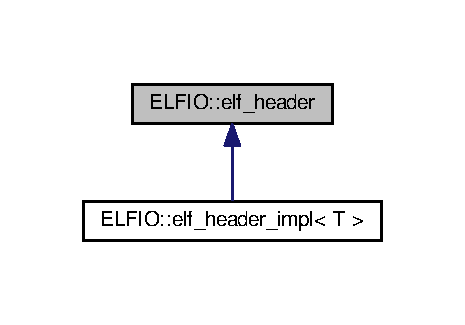
\includegraphics[width=223pt]{class_e_l_f_i_o_1_1elf__header__inherit__graph}
\end{center}
\end{figure}
\subsection*{Public Member Functions}
\begin{DoxyCompactItemize}
\item 
virtual bool {\bfseries load} (std\+::istream \&stream)=0\hypertarget{class_e_l_f_i_o_1_1elf__header_ab4d46f817a381c214901d83e20e8f105}{}\label{class_e_l_f_i_o_1_1elf__header_ab4d46f817a381c214901d83e20e8f105}

\item 
virtual bool {\bfseries save} (std\+::ostream \&stream) const =0\hypertarget{class_e_l_f_i_o_1_1elf__header_a4ddc14a74b4d2e919ba300f88ea90af6}{}\label{class_e_l_f_i_o_1_1elf__header_a4ddc14a74b4d2e919ba300f88ea90af6}

\item 
{\bfseries E\+L\+F\+I\+O\+\_\+\+G\+E\+T\+\_\+\+A\+C\+C\+E\+S\+S\+\_\+\+D\+E\+CL} (unsigned char, class)\hypertarget{class_e_l_f_i_o_1_1elf__header_adce7e1366bd9400318ade778f6ad26c4}{}\label{class_e_l_f_i_o_1_1elf__header_adce7e1366bd9400318ade778f6ad26c4}

\item 
{\bfseries E\+L\+F\+I\+O\+\_\+\+G\+E\+T\+\_\+\+A\+C\+C\+E\+S\+S\+\_\+\+D\+E\+CL} (unsigned char, elf\+\_\+version)\hypertarget{class_e_l_f_i_o_1_1elf__header_a56f22ab07bfcf305cc9c07e51d2fef82}{}\label{class_e_l_f_i_o_1_1elf__header_a56f22ab07bfcf305cc9c07e51d2fef82}

\item 
{\bfseries E\+L\+F\+I\+O\+\_\+\+G\+E\+T\+\_\+\+A\+C\+C\+E\+S\+S\+\_\+\+D\+E\+CL} (unsigned char, encoding)\hypertarget{class_e_l_f_i_o_1_1elf__header_a8dff580e4e0c0a54c75c08711a0b7ef0}{}\label{class_e_l_f_i_o_1_1elf__header_a8dff580e4e0c0a54c75c08711a0b7ef0}

\item 
{\bfseries E\+L\+F\+I\+O\+\_\+\+G\+E\+T\+\_\+\+A\+C\+C\+E\+S\+S\+\_\+\+D\+E\+CL} (Elf\+\_\+\+Word, version)\hypertarget{class_e_l_f_i_o_1_1elf__header_a3f317ed2516b5357203a78cf050a2739}{}\label{class_e_l_f_i_o_1_1elf__header_a3f317ed2516b5357203a78cf050a2739}

\item 
{\bfseries E\+L\+F\+I\+O\+\_\+\+G\+E\+T\+\_\+\+A\+C\+C\+E\+S\+S\+\_\+\+D\+E\+CL} (Elf\+\_\+\+Half, header\+\_\+size)\hypertarget{class_e_l_f_i_o_1_1elf__header_a9a99ed072d5c453885515b6b66cd589a}{}\label{class_e_l_f_i_o_1_1elf__header_a9a99ed072d5c453885515b6b66cd589a}

\item 
{\bfseries E\+L\+F\+I\+O\+\_\+\+G\+E\+T\+\_\+\+A\+C\+C\+E\+S\+S\+\_\+\+D\+E\+CL} (Elf\+\_\+\+Half, section\+\_\+entry\+\_\+size)\hypertarget{class_e_l_f_i_o_1_1elf__header_a9acbc16b6ae72ab36d994202e8318fbc}{}\label{class_e_l_f_i_o_1_1elf__header_a9acbc16b6ae72ab36d994202e8318fbc}

\item 
{\bfseries E\+L\+F\+I\+O\+\_\+\+G\+E\+T\+\_\+\+A\+C\+C\+E\+S\+S\+\_\+\+D\+E\+CL} (Elf\+\_\+\+Half, segment\+\_\+entry\+\_\+size)\hypertarget{class_e_l_f_i_o_1_1elf__header_a27fdb0ac591e8d2fed4c30a9da83b161}{}\label{class_e_l_f_i_o_1_1elf__header_a27fdb0ac591e8d2fed4c30a9da83b161}

\item 
{\bfseries E\+L\+F\+I\+O\+\_\+\+G\+E\+T\+\_\+\+S\+E\+T\+\_\+\+A\+C\+C\+E\+S\+S\+\_\+\+D\+E\+CL} (unsigned char, os\+\_\+abi)\hypertarget{class_e_l_f_i_o_1_1elf__header_aeb82c28cee1d098696fd422ba47767ba}{}\label{class_e_l_f_i_o_1_1elf__header_aeb82c28cee1d098696fd422ba47767ba}

\item 
{\bfseries E\+L\+F\+I\+O\+\_\+\+G\+E\+T\+\_\+\+S\+E\+T\+\_\+\+A\+C\+C\+E\+S\+S\+\_\+\+D\+E\+CL} (unsigned char, abi\+\_\+version)\hypertarget{class_e_l_f_i_o_1_1elf__header_a48784e215429b29fc0f99cbc1c4da43a}{}\label{class_e_l_f_i_o_1_1elf__header_a48784e215429b29fc0f99cbc1c4da43a}

\item 
{\bfseries E\+L\+F\+I\+O\+\_\+\+G\+E\+T\+\_\+\+S\+E\+T\+\_\+\+A\+C\+C\+E\+S\+S\+\_\+\+D\+E\+CL} (Elf\+\_\+\+Half, type)\hypertarget{class_e_l_f_i_o_1_1elf__header_a951284ab4a8e285e0b0668c534bbed60}{}\label{class_e_l_f_i_o_1_1elf__header_a951284ab4a8e285e0b0668c534bbed60}

\item 
{\bfseries E\+L\+F\+I\+O\+\_\+\+G\+E\+T\+\_\+\+S\+E\+T\+\_\+\+A\+C\+C\+E\+S\+S\+\_\+\+D\+E\+CL} (Elf\+\_\+\+Half, machine)\hypertarget{class_e_l_f_i_o_1_1elf__header_a25882d82b5a01e3f28e10a76e3986776}{}\label{class_e_l_f_i_o_1_1elf__header_a25882d82b5a01e3f28e10a76e3986776}

\item 
{\bfseries E\+L\+F\+I\+O\+\_\+\+G\+E\+T\+\_\+\+S\+E\+T\+\_\+\+A\+C\+C\+E\+S\+S\+\_\+\+D\+E\+CL} (Elf\+\_\+\+Word, flags)\hypertarget{class_e_l_f_i_o_1_1elf__header_a27fe3dbfa7ef6f7de22accf35cab00ab}{}\label{class_e_l_f_i_o_1_1elf__header_a27fe3dbfa7ef6f7de22accf35cab00ab}

\item 
{\bfseries E\+L\+F\+I\+O\+\_\+\+G\+E\+T\+\_\+\+S\+E\+T\+\_\+\+A\+C\+C\+E\+S\+S\+\_\+\+D\+E\+CL} (Elf64\+\_\+\+Addr, entry)\hypertarget{class_e_l_f_i_o_1_1elf__header_aab270cef87e0d7f044724c8078500d9d}{}\label{class_e_l_f_i_o_1_1elf__header_aab270cef87e0d7f044724c8078500d9d}

\item 
{\bfseries E\+L\+F\+I\+O\+\_\+\+G\+E\+T\+\_\+\+S\+E\+T\+\_\+\+A\+C\+C\+E\+S\+S\+\_\+\+D\+E\+CL} (Elf\+\_\+\+Half, sections\+\_\+num)\hypertarget{class_e_l_f_i_o_1_1elf__header_a4cccb54184ca67532cad18898ffddd57}{}\label{class_e_l_f_i_o_1_1elf__header_a4cccb54184ca67532cad18898ffddd57}

\item 
{\bfseries E\+L\+F\+I\+O\+\_\+\+G\+E\+T\+\_\+\+S\+E\+T\+\_\+\+A\+C\+C\+E\+S\+S\+\_\+\+D\+E\+CL} (Elf64\+\_\+\+Off, sections\+\_\+offset)\hypertarget{class_e_l_f_i_o_1_1elf__header_aab88310d486cc319b37730b8a658a6fd}{}\label{class_e_l_f_i_o_1_1elf__header_aab88310d486cc319b37730b8a658a6fd}

\item 
{\bfseries E\+L\+F\+I\+O\+\_\+\+G\+E\+T\+\_\+\+S\+E\+T\+\_\+\+A\+C\+C\+E\+S\+S\+\_\+\+D\+E\+CL} (Elf\+\_\+\+Half, segments\+\_\+num)\hypertarget{class_e_l_f_i_o_1_1elf__header_aafcebb8735be7a5791d1ee3956329bc0}{}\label{class_e_l_f_i_o_1_1elf__header_aafcebb8735be7a5791d1ee3956329bc0}

\item 
{\bfseries E\+L\+F\+I\+O\+\_\+\+G\+E\+T\+\_\+\+S\+E\+T\+\_\+\+A\+C\+C\+E\+S\+S\+\_\+\+D\+E\+CL} (Elf64\+\_\+\+Off, segments\+\_\+offset)\hypertarget{class_e_l_f_i_o_1_1elf__header_a3e722fc7b7c47e8aedaaa00966099901}{}\label{class_e_l_f_i_o_1_1elf__header_a3e722fc7b7c47e8aedaaa00966099901}

\item 
{\bfseries E\+L\+F\+I\+O\+\_\+\+G\+E\+T\+\_\+\+S\+E\+T\+\_\+\+A\+C\+C\+E\+S\+S\+\_\+\+D\+E\+CL} (Elf\+\_\+\+Half, section\+\_\+name\+\_\+str\+\_\+index)\hypertarget{class_e_l_f_i_o_1_1elf__header_a995676c92a356608b21dbd7db7f4cd51}{}\label{class_e_l_f_i_o_1_1elf__header_a995676c92a356608b21dbd7db7f4cd51}

\end{DoxyCompactItemize}


The documentation for this class was generated from the following file\+:\begin{DoxyCompactItemize}
\item 
include/elfio/elfio\+\_\+header.\+hpp\end{DoxyCompactItemize}

\hypertarget{class_e_l_f_i_o_1_1elf__header__impl}{}\section{E\+L\+F\+IO\+:\+:elf\+\_\+header\+\_\+impl$<$ T $>$ Class Template Reference}
\label{class_e_l_f_i_o_1_1elf__header__impl}\index{E\+L\+F\+I\+O\+::elf\+\_\+header\+\_\+impl$<$ T $>$@{E\+L\+F\+I\+O\+::elf\+\_\+header\+\_\+impl$<$ T $>$}}


Inheritance diagram for E\+L\+F\+IO\+:\+:elf\+\_\+header\+\_\+impl$<$ T $>$\+:\nopagebreak
\begin{figure}[H]
\begin{center}
\leavevmode
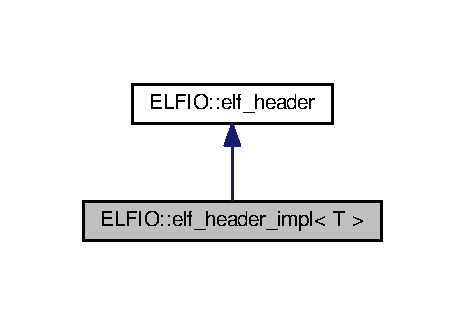
\includegraphics[width=223pt]{class_e_l_f_i_o_1_1elf__header__impl__inherit__graph}
\end{center}
\end{figure}


Collaboration diagram for E\+L\+F\+IO\+:\+:elf\+\_\+header\+\_\+impl$<$ T $>$\+:\nopagebreak
\begin{figure}[H]
\begin{center}
\leavevmode
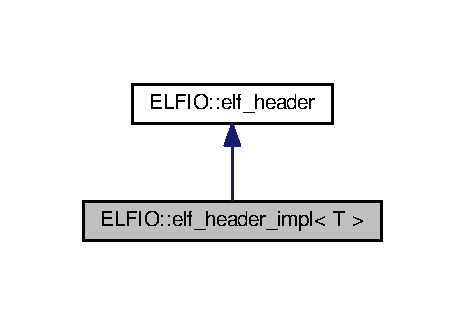
\includegraphics[width=223pt]{class_e_l_f_i_o_1_1elf__header__impl__coll__graph}
\end{center}
\end{figure}
\subsection*{Public Member Functions}
\begin{DoxyCompactItemize}
\item 
{\bfseries elf\+\_\+header\+\_\+impl} (\hyperlink{class_e_l_f_i_o_1_1endianess__convertor}{endianess\+\_\+convertor} $\ast$convertor\+\_\+, unsigned char encoding)\hypertarget{class_e_l_f_i_o_1_1elf__header__impl_a9b0d14138c2321771d6e58d0da2b8835}{}\label{class_e_l_f_i_o_1_1elf__header__impl_a9b0d14138c2321771d6e58d0da2b8835}

\item 
bool {\bfseries load} (std\+::istream \&stream)\hypertarget{class_e_l_f_i_o_1_1elf__header__impl_a5a94421ae7a4de702962db1f0d4cbc4a}{}\label{class_e_l_f_i_o_1_1elf__header__impl_a5a94421ae7a4de702962db1f0d4cbc4a}

\item 
bool {\bfseries save} (std\+::ostream \&stream) const \hypertarget{class_e_l_f_i_o_1_1elf__header__impl_afcabc009094d0328a95ddc2672dd774a}{}\label{class_e_l_f_i_o_1_1elf__header__impl_afcabc009094d0328a95ddc2672dd774a}

\item 
{\bfseries E\+L\+F\+I\+O\+\_\+\+G\+E\+T\+\_\+\+A\+C\+C\+E\+SS} (unsigned char, class, header.\+e\+\_\+ident\mbox{[}E\+I\+\_\+\+C\+L\+A\+SS\mbox{]})\hypertarget{class_e_l_f_i_o_1_1elf__header__impl_ae72b38f4d5cf6aa371a38b7dce94c827}{}\label{class_e_l_f_i_o_1_1elf__header__impl_ae72b38f4d5cf6aa371a38b7dce94c827}

\item 
{\bfseries E\+L\+F\+I\+O\+\_\+\+G\+E\+T\+\_\+\+A\+C\+C\+E\+SS} (unsigned char, elf\+\_\+version, header.\+e\+\_\+ident\mbox{[}E\+I\+\_\+\+V\+E\+R\+S\+I\+ON\mbox{]})\hypertarget{class_e_l_f_i_o_1_1elf__header__impl_a39341c9d4881f1315ff0005e2324e9dc}{}\label{class_e_l_f_i_o_1_1elf__header__impl_a39341c9d4881f1315ff0005e2324e9dc}

\item 
{\bfseries E\+L\+F\+I\+O\+\_\+\+G\+E\+T\+\_\+\+A\+C\+C\+E\+SS} (unsigned char, encoding, header.\+e\+\_\+ident\mbox{[}E\+I\+\_\+\+D\+A\+TA\mbox{]})\hypertarget{class_e_l_f_i_o_1_1elf__header__impl_a29197b16468fa1f7bb04d753a117ec3a}{}\label{class_e_l_f_i_o_1_1elf__header__impl_a29197b16468fa1f7bb04d753a117ec3a}

\item 
{\bfseries E\+L\+F\+I\+O\+\_\+\+G\+E\+T\+\_\+\+A\+C\+C\+E\+SS} (Elf\+\_\+\+Word, version, header.\+e\+\_\+version)\hypertarget{class_e_l_f_i_o_1_1elf__header__impl_a9eaa837636983deddf78526f828c03ee}{}\label{class_e_l_f_i_o_1_1elf__header__impl_a9eaa837636983deddf78526f828c03ee}

\item 
{\bfseries E\+L\+F\+I\+O\+\_\+\+G\+E\+T\+\_\+\+A\+C\+C\+E\+SS} (Elf\+\_\+\+Half, header\+\_\+size, header.\+e\+\_\+ehsize)\hypertarget{class_e_l_f_i_o_1_1elf__header__impl_a6cf004e0d0c14a242cc17fc55cdac7a0}{}\label{class_e_l_f_i_o_1_1elf__header__impl_a6cf004e0d0c14a242cc17fc55cdac7a0}

\item 
{\bfseries E\+L\+F\+I\+O\+\_\+\+G\+E\+T\+\_\+\+A\+C\+C\+E\+SS} (Elf\+\_\+\+Half, section\+\_\+entry\+\_\+size, header.\+e\+\_\+shentsize)\hypertarget{class_e_l_f_i_o_1_1elf__header__impl_a10dec874c12e705e9897c6b231f6808a}{}\label{class_e_l_f_i_o_1_1elf__header__impl_a10dec874c12e705e9897c6b231f6808a}

\item 
{\bfseries E\+L\+F\+I\+O\+\_\+\+G\+E\+T\+\_\+\+A\+C\+C\+E\+SS} (Elf\+\_\+\+Half, segment\+\_\+entry\+\_\+size, header.\+e\+\_\+phentsize)\hypertarget{class_e_l_f_i_o_1_1elf__header__impl_a25c45d46c5ead97a253675cd94c27144}{}\label{class_e_l_f_i_o_1_1elf__header__impl_a25c45d46c5ead97a253675cd94c27144}

\item 
{\bfseries E\+L\+F\+I\+O\+\_\+\+G\+E\+T\+\_\+\+S\+E\+T\+\_\+\+A\+C\+C\+E\+SS} (unsigned char, os\+\_\+abi, header.\+e\+\_\+ident\mbox{[}E\+I\+\_\+\+O\+S\+A\+BI\mbox{]})\hypertarget{class_e_l_f_i_o_1_1elf__header__impl_aebdf9365324c5da906e322640902e6f0}{}\label{class_e_l_f_i_o_1_1elf__header__impl_aebdf9365324c5da906e322640902e6f0}

\item 
{\bfseries E\+L\+F\+I\+O\+\_\+\+G\+E\+T\+\_\+\+S\+E\+T\+\_\+\+A\+C\+C\+E\+SS} (unsigned char, abi\+\_\+version, header.\+e\+\_\+ident\mbox{[}E\+I\+\_\+\+A\+B\+I\+V\+E\+R\+S\+I\+ON\mbox{]})\hypertarget{class_e_l_f_i_o_1_1elf__header__impl_ac7df14428cbf48762e07fba690f9abe9}{}\label{class_e_l_f_i_o_1_1elf__header__impl_ac7df14428cbf48762e07fba690f9abe9}

\item 
{\bfseries E\+L\+F\+I\+O\+\_\+\+G\+E\+T\+\_\+\+S\+E\+T\+\_\+\+A\+C\+C\+E\+SS} (Elf\+\_\+\+Half, type, header.\+e\+\_\+type)\hypertarget{class_e_l_f_i_o_1_1elf__header__impl_a052ff49b5435203764c9ead3a7bc9594}{}\label{class_e_l_f_i_o_1_1elf__header__impl_a052ff49b5435203764c9ead3a7bc9594}

\item 
{\bfseries E\+L\+F\+I\+O\+\_\+\+G\+E\+T\+\_\+\+S\+E\+T\+\_\+\+A\+C\+C\+E\+SS} (Elf\+\_\+\+Half, machine, header.\+e\+\_\+machine)\hypertarget{class_e_l_f_i_o_1_1elf__header__impl_a6c9d93feb68b4b6c174721e1f2119a65}{}\label{class_e_l_f_i_o_1_1elf__header__impl_a6c9d93feb68b4b6c174721e1f2119a65}

\item 
{\bfseries E\+L\+F\+I\+O\+\_\+\+G\+E\+T\+\_\+\+S\+E\+T\+\_\+\+A\+C\+C\+E\+SS} (Elf\+\_\+\+Word, flags, header.\+e\+\_\+flags)\hypertarget{class_e_l_f_i_o_1_1elf__header__impl_ae29a839a52a29c630e7dd6739796acde}{}\label{class_e_l_f_i_o_1_1elf__header__impl_ae29a839a52a29c630e7dd6739796acde}

\item 
{\bfseries E\+L\+F\+I\+O\+\_\+\+G\+E\+T\+\_\+\+S\+E\+T\+\_\+\+A\+C\+C\+E\+SS} (Elf\+\_\+\+Half, section\+\_\+name\+\_\+str\+\_\+index, header.\+e\+\_\+shstrndx)\hypertarget{class_e_l_f_i_o_1_1elf__header__impl_a799c1da8737df93af47a17eae3e06f2a}{}\label{class_e_l_f_i_o_1_1elf__header__impl_a799c1da8737df93af47a17eae3e06f2a}

\item 
{\bfseries E\+L\+F\+I\+O\+\_\+\+G\+E\+T\+\_\+\+S\+E\+T\+\_\+\+A\+C\+C\+E\+SS} (Elf64\+\_\+\+Addr, entry, header.\+e\+\_\+entry)\hypertarget{class_e_l_f_i_o_1_1elf__header__impl_ad9d2bface2469e6ad79bed1b7347b7d3}{}\label{class_e_l_f_i_o_1_1elf__header__impl_ad9d2bface2469e6ad79bed1b7347b7d3}

\item 
{\bfseries E\+L\+F\+I\+O\+\_\+\+G\+E\+T\+\_\+\+S\+E\+T\+\_\+\+A\+C\+C\+E\+SS} (Elf\+\_\+\+Half, sections\+\_\+num, header.\+e\+\_\+shnum)\hypertarget{class_e_l_f_i_o_1_1elf__header__impl_ac58fc37a8cee60af02dd2a7f18dea170}{}\label{class_e_l_f_i_o_1_1elf__header__impl_ac58fc37a8cee60af02dd2a7f18dea170}

\item 
{\bfseries E\+L\+F\+I\+O\+\_\+\+G\+E\+T\+\_\+\+S\+E\+T\+\_\+\+A\+C\+C\+E\+SS} (Elf64\+\_\+\+Off, sections\+\_\+offset, header.\+e\+\_\+shoff)\hypertarget{class_e_l_f_i_o_1_1elf__header__impl_af7b4de848c45269f7a4405b7158ba67a}{}\label{class_e_l_f_i_o_1_1elf__header__impl_af7b4de848c45269f7a4405b7158ba67a}

\item 
{\bfseries E\+L\+F\+I\+O\+\_\+\+G\+E\+T\+\_\+\+S\+E\+T\+\_\+\+A\+C\+C\+E\+SS} (Elf\+\_\+\+Half, segments\+\_\+num, header.\+e\+\_\+phnum)\hypertarget{class_e_l_f_i_o_1_1elf__header__impl_ac83e843ac1c5493235b990a50b7373bb}{}\label{class_e_l_f_i_o_1_1elf__header__impl_ac83e843ac1c5493235b990a50b7373bb}

\item 
{\bfseries E\+L\+F\+I\+O\+\_\+\+G\+E\+T\+\_\+\+S\+E\+T\+\_\+\+A\+C\+C\+E\+SS} (Elf64\+\_\+\+Off, segments\+\_\+offset, header.\+e\+\_\+phoff)\hypertarget{class_e_l_f_i_o_1_1elf__header__impl_a7a0c56190c9f5f9b32afa52d15ea1c94}{}\label{class_e_l_f_i_o_1_1elf__header__impl_a7a0c56190c9f5f9b32afa52d15ea1c94}

\end{DoxyCompactItemize}


The documentation for this class was generated from the following file\+:\begin{DoxyCompactItemize}
\item 
include/elfio/elfio\+\_\+header.\+hpp\end{DoxyCompactItemize}

\hypertarget{struct_e_l_f_i_o_1_1elf__header__impl__types}{}\section{E\+L\+F\+IO\+:\+:elf\+\_\+header\+\_\+impl\+\_\+types$<$ T $>$ Struct Template Reference}
\label{struct_e_l_f_i_o_1_1elf__header__impl__types}\index{E\+L\+F\+I\+O\+::elf\+\_\+header\+\_\+impl\+\_\+types$<$ T $>$@{E\+L\+F\+I\+O\+::elf\+\_\+header\+\_\+impl\+\_\+types$<$ T $>$}}


The documentation for this struct was generated from the following file\+:\begin{DoxyCompactItemize}
\item 
include/elfio/elfio\+\_\+header.\+hpp\end{DoxyCompactItemize}

\hypertarget{struct_e_l_f_i_o_1_1elf__header__impl__types_3_01_elf32___ehdr_01_4}{}\section{E\+L\+F\+IO\+:\+:elf\+\_\+header\+\_\+impl\+\_\+types$<$ Elf32\+\_\+\+Ehdr $>$ Struct Template Reference}
\label{struct_e_l_f_i_o_1_1elf__header__impl__types_3_01_elf32___ehdr_01_4}\index{E\+L\+F\+I\+O\+::elf\+\_\+header\+\_\+impl\+\_\+types$<$ Elf32\+\_\+\+Ehdr $>$@{E\+L\+F\+I\+O\+::elf\+\_\+header\+\_\+impl\+\_\+types$<$ Elf32\+\_\+\+Ehdr $>$}}
\subsection*{Public Types}
\begin{DoxyCompactItemize}
\item 
typedef \hyperlink{struct_e_l_f_i_o_1_1_elf32___phdr}{Elf32\+\_\+\+Phdr} {\bfseries Phdr\+\_\+type}\hypertarget{struct_e_l_f_i_o_1_1elf__header__impl__types_3_01_elf32___ehdr_01_4_a29863b014dcfb409b9e7063dcbedfdcd}{}\label{struct_e_l_f_i_o_1_1elf__header__impl__types_3_01_elf32___ehdr_01_4_a29863b014dcfb409b9e7063dcbedfdcd}

\item 
typedef \hyperlink{struct_e_l_f_i_o_1_1_elf32___shdr}{Elf32\+\_\+\+Shdr} {\bfseries Shdr\+\_\+type}\hypertarget{struct_e_l_f_i_o_1_1elf__header__impl__types_3_01_elf32___ehdr_01_4_ac5cf48a8698f0f7947677e306784aace}{}\label{struct_e_l_f_i_o_1_1elf__header__impl__types_3_01_elf32___ehdr_01_4_ac5cf48a8698f0f7947677e306784aace}

\end{DoxyCompactItemize}
\subsection*{Static Public Attributes}
\begin{DoxyCompactItemize}
\item 
static const unsigned char {\bfseries file\+\_\+class} = E\+L\+F\+C\+L\+A\+S\+S32\hypertarget{struct_e_l_f_i_o_1_1elf__header__impl__types_3_01_elf32___ehdr_01_4_a98a44bc25c8487143bda120bbb8d602b}{}\label{struct_e_l_f_i_o_1_1elf__header__impl__types_3_01_elf32___ehdr_01_4_a98a44bc25c8487143bda120bbb8d602b}

\end{DoxyCompactItemize}


The documentation for this struct was generated from the following file\+:\begin{DoxyCompactItemize}
\item 
include/elfio/elfio\+\_\+header.\+hpp\end{DoxyCompactItemize}

\hypertarget{struct_e_l_f_i_o_1_1elf__header__impl__types_3_01_elf64___ehdr_01_4}{}\section{E\+L\+F\+IO\+:\+:elf\+\_\+header\+\_\+impl\+\_\+types$<$ Elf64\+\_\+\+Ehdr $>$ Struct Template Reference}
\label{struct_e_l_f_i_o_1_1elf__header__impl__types_3_01_elf64___ehdr_01_4}\index{E\+L\+F\+I\+O\+::elf\+\_\+header\+\_\+impl\+\_\+types$<$ Elf64\+\_\+\+Ehdr $>$@{E\+L\+F\+I\+O\+::elf\+\_\+header\+\_\+impl\+\_\+types$<$ Elf64\+\_\+\+Ehdr $>$}}
\subsection*{Public Types}
\begin{DoxyCompactItemize}
\item 
typedef \hyperlink{struct_e_l_f_i_o_1_1_elf64___phdr}{Elf64\+\_\+\+Phdr} {\bfseries Phdr\+\_\+type}\hypertarget{struct_e_l_f_i_o_1_1elf__header__impl__types_3_01_elf64___ehdr_01_4_adb25fa9e29790704c42240aeeb47c3ae}{}\label{struct_e_l_f_i_o_1_1elf__header__impl__types_3_01_elf64___ehdr_01_4_adb25fa9e29790704c42240aeeb47c3ae}

\item 
typedef \hyperlink{struct_e_l_f_i_o_1_1_elf64___shdr}{Elf64\+\_\+\+Shdr} {\bfseries Shdr\+\_\+type}\hypertarget{struct_e_l_f_i_o_1_1elf__header__impl__types_3_01_elf64___ehdr_01_4_aa4b7b8e2f0ef6bdb750c0044ef8ec174}{}\label{struct_e_l_f_i_o_1_1elf__header__impl__types_3_01_elf64___ehdr_01_4_aa4b7b8e2f0ef6bdb750c0044ef8ec174}

\end{DoxyCompactItemize}
\subsection*{Static Public Attributes}
\begin{DoxyCompactItemize}
\item 
static const unsigned char {\bfseries file\+\_\+class} = E\+L\+F\+C\+L\+A\+S\+S64\hypertarget{struct_e_l_f_i_o_1_1elf__header__impl__types_3_01_elf64___ehdr_01_4_aeea4dcb067d1745cd80aa6e810adf214}{}\label{struct_e_l_f_i_o_1_1elf__header__impl__types_3_01_elf64___ehdr_01_4_aeea4dcb067d1745cd80aa6e810adf214}

\end{DoxyCompactItemize}


The documentation for this struct was generated from the following file\+:\begin{DoxyCompactItemize}
\item 
include/elfio/elfio\+\_\+header.\+hpp\end{DoxyCompactItemize}

\hypertarget{class_e_l_f_i_o_1_1elfio}{}\section{E\+L\+F\+IO\+:\+:elfio Class Reference}
\label{class_e_l_f_i_o_1_1elfio}\index{E\+L\+F\+I\+O\+::elfio@{E\+L\+F\+I\+O\+::elfio}}


Collaboration diagram for E\+L\+F\+IO\+:\+:elfio\+:\nopagebreak
\begin{figure}[H]
\begin{center}
\leavevmode
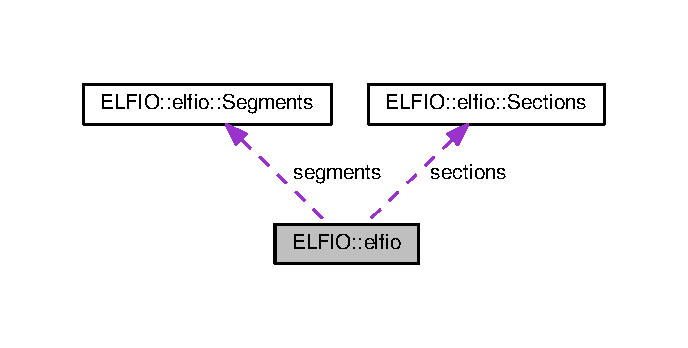
\includegraphics[width=330pt]{class_e_l_f_i_o_1_1elfio__coll__graph}
\end{center}
\end{figure}
\subsection*{Classes}
\begin{DoxyCompactItemize}
\item 
class \hyperlink{class_e_l_f_i_o_1_1elfio_1_1_sections}{Sections}
\item 
class \hyperlink{class_e_l_f_i_o_1_1elfio_1_1_segments}{Segments}
\end{DoxyCompactItemize}
\subsection*{Public Member Functions}
\begin{DoxyCompactItemize}
\item 
void {\bfseries create} (unsigned char file\+\_\+class, unsigned char encoding)\hypertarget{class_e_l_f_i_o_1_1elfio_a505f88e23277cb7945d4f411fe2b4d85}{}\label{class_e_l_f_i_o_1_1elfio_a505f88e23277cb7945d4f411fe2b4d85}

\item 
bool {\bfseries load} (const std\+::string \&file\+\_\+name)\hypertarget{class_e_l_f_i_o_1_1elfio_af313dfceaf57ca8342e1cebba19a986e}{}\label{class_e_l_f_i_o_1_1elfio_af313dfceaf57ca8342e1cebba19a986e}

\item 
bool {\bfseries load} (std\+::istream \&stream)\hypertarget{class_e_l_f_i_o_1_1elfio_a1eb421b95b3deb91f7e4c28cbf094614}{}\label{class_e_l_f_i_o_1_1elfio_a1eb421b95b3deb91f7e4c28cbf094614}

\item 
bool {\bfseries save} (const std\+::string \&file\+\_\+name)\hypertarget{class_e_l_f_i_o_1_1elfio_a4dfd167b10c72779390871865d16db61}{}\label{class_e_l_f_i_o_1_1elfio_a4dfd167b10c72779390871865d16db61}

\item 
{\bfseries E\+L\+F\+I\+O\+\_\+\+H\+E\+A\+D\+E\+R\+\_\+\+A\+C\+C\+E\+S\+S\+\_\+\+G\+ET} (unsigned char, class)\hypertarget{class_e_l_f_i_o_1_1elfio_a45ae995bbe7d5e483aeac5ff87919fe5}{}\label{class_e_l_f_i_o_1_1elfio_a45ae995bbe7d5e483aeac5ff87919fe5}

\item 
{\bfseries E\+L\+F\+I\+O\+\_\+\+H\+E\+A\+D\+E\+R\+\_\+\+A\+C\+C\+E\+S\+S\+\_\+\+G\+ET} (unsigned char, elf\+\_\+version)\hypertarget{class_e_l_f_i_o_1_1elfio_a20456cc1e0bf4600acc7d17ee7cdf5d3}{}\label{class_e_l_f_i_o_1_1elfio_a20456cc1e0bf4600acc7d17ee7cdf5d3}

\item 
{\bfseries E\+L\+F\+I\+O\+\_\+\+H\+E\+A\+D\+E\+R\+\_\+\+A\+C\+C\+E\+S\+S\+\_\+\+G\+ET} (unsigned char, encoding)\hypertarget{class_e_l_f_i_o_1_1elfio_a327474e3c1233af704e0bfd8b03c4380}{}\label{class_e_l_f_i_o_1_1elfio_a327474e3c1233af704e0bfd8b03c4380}

\item 
{\bfseries E\+L\+F\+I\+O\+\_\+\+H\+E\+A\+D\+E\+R\+\_\+\+A\+C\+C\+E\+S\+S\+\_\+\+G\+ET} (Elf\+\_\+\+Word, version)\hypertarget{class_e_l_f_i_o_1_1elfio_a41de7411abbe40fd2c4d9758f71794d6}{}\label{class_e_l_f_i_o_1_1elfio_a41de7411abbe40fd2c4d9758f71794d6}

\item 
{\bfseries E\+L\+F\+I\+O\+\_\+\+H\+E\+A\+D\+E\+R\+\_\+\+A\+C\+C\+E\+S\+S\+\_\+\+G\+ET} (Elf\+\_\+\+Half, header\+\_\+size)\hypertarget{class_e_l_f_i_o_1_1elfio_a724c168431bfc57f2971dd639e7562f6}{}\label{class_e_l_f_i_o_1_1elfio_a724c168431bfc57f2971dd639e7562f6}

\item 
{\bfseries E\+L\+F\+I\+O\+\_\+\+H\+E\+A\+D\+E\+R\+\_\+\+A\+C\+C\+E\+S\+S\+\_\+\+G\+ET} (Elf\+\_\+\+Half, section\+\_\+entry\+\_\+size)\hypertarget{class_e_l_f_i_o_1_1elfio_a4ef6cb10ed0603f5827dc24e4263bc71}{}\label{class_e_l_f_i_o_1_1elfio_a4ef6cb10ed0603f5827dc24e4263bc71}

\item 
{\bfseries E\+L\+F\+I\+O\+\_\+\+H\+E\+A\+D\+E\+R\+\_\+\+A\+C\+C\+E\+S\+S\+\_\+\+G\+ET} (Elf\+\_\+\+Half, segment\+\_\+entry\+\_\+size)\hypertarget{class_e_l_f_i_o_1_1elfio_aaaaaace05a2318b072cba732fdaf31f1}{}\label{class_e_l_f_i_o_1_1elfio_aaaaaace05a2318b072cba732fdaf31f1}

\item 
{\bfseries E\+L\+F\+I\+O\+\_\+\+H\+E\+A\+D\+E\+R\+\_\+\+A\+C\+C\+E\+S\+S\+\_\+\+G\+E\+T\+\_\+\+S\+ET} (unsigned char, os\+\_\+abi)\hypertarget{class_e_l_f_i_o_1_1elfio_a402231bc0fcfaade53ac1a00d03b1beb}{}\label{class_e_l_f_i_o_1_1elfio_a402231bc0fcfaade53ac1a00d03b1beb}

\item 
{\bfseries E\+L\+F\+I\+O\+\_\+\+H\+E\+A\+D\+E\+R\+\_\+\+A\+C\+C\+E\+S\+S\+\_\+\+G\+E\+T\+\_\+\+S\+ET} (unsigned char, abi\+\_\+version)\hypertarget{class_e_l_f_i_o_1_1elfio_a7a0af3403557d27bab40327fd77694d5}{}\label{class_e_l_f_i_o_1_1elfio_a7a0af3403557d27bab40327fd77694d5}

\item 
{\bfseries E\+L\+F\+I\+O\+\_\+\+H\+E\+A\+D\+E\+R\+\_\+\+A\+C\+C\+E\+S\+S\+\_\+\+G\+E\+T\+\_\+\+S\+ET} (Elf\+\_\+\+Half, type)\hypertarget{class_e_l_f_i_o_1_1elfio_a62ff13bb90d932c129d7a9cee7f3fe0d}{}\label{class_e_l_f_i_o_1_1elfio_a62ff13bb90d932c129d7a9cee7f3fe0d}

\item 
{\bfseries E\+L\+F\+I\+O\+\_\+\+H\+E\+A\+D\+E\+R\+\_\+\+A\+C\+C\+E\+S\+S\+\_\+\+G\+E\+T\+\_\+\+S\+ET} (Elf\+\_\+\+Half, machine)\hypertarget{class_e_l_f_i_o_1_1elfio_a4c490e4dad96669132fb194809b3c1ca}{}\label{class_e_l_f_i_o_1_1elfio_a4c490e4dad96669132fb194809b3c1ca}

\item 
{\bfseries E\+L\+F\+I\+O\+\_\+\+H\+E\+A\+D\+E\+R\+\_\+\+A\+C\+C\+E\+S\+S\+\_\+\+G\+E\+T\+\_\+\+S\+ET} (Elf\+\_\+\+Word, flags)\hypertarget{class_e_l_f_i_o_1_1elfio_ad4886c3772461b05596575735a6fc155}{}\label{class_e_l_f_i_o_1_1elfio_ad4886c3772461b05596575735a6fc155}

\item 
{\bfseries E\+L\+F\+I\+O\+\_\+\+H\+E\+A\+D\+E\+R\+\_\+\+A\+C\+C\+E\+S\+S\+\_\+\+G\+E\+T\+\_\+\+S\+ET} (Elf64\+\_\+\+Addr, entry)\hypertarget{class_e_l_f_i_o_1_1elfio_a2d7c2d21ce1f1ee5594223a5e9c0ec0c}{}\label{class_e_l_f_i_o_1_1elfio_a2d7c2d21ce1f1ee5594223a5e9c0ec0c}

\item 
{\bfseries E\+L\+F\+I\+O\+\_\+\+H\+E\+A\+D\+E\+R\+\_\+\+A\+C\+C\+E\+S\+S\+\_\+\+G\+E\+T\+\_\+\+S\+ET} (Elf64\+\_\+\+Off, sections\+\_\+offset)\hypertarget{class_e_l_f_i_o_1_1elfio_a8c5153e5b46bb52de27e6a2a9ec54284}{}\label{class_e_l_f_i_o_1_1elfio_a8c5153e5b46bb52de27e6a2a9ec54284}

\item 
{\bfseries E\+L\+F\+I\+O\+\_\+\+H\+E\+A\+D\+E\+R\+\_\+\+A\+C\+C\+E\+S\+S\+\_\+\+G\+E\+T\+\_\+\+S\+ET} (Elf64\+\_\+\+Off, segments\+\_\+offset)\hypertarget{class_e_l_f_i_o_1_1elfio_aeab9eea10af4a4bac5c286ec910fc7d9}{}\label{class_e_l_f_i_o_1_1elfio_aeab9eea10af4a4bac5c286ec910fc7d9}

\item 
{\bfseries E\+L\+F\+I\+O\+\_\+\+H\+E\+A\+D\+E\+R\+\_\+\+A\+C\+C\+E\+S\+S\+\_\+\+G\+E\+T\+\_\+\+S\+ET} (Elf\+\_\+\+Half, section\+\_\+name\+\_\+str\+\_\+index)\hypertarget{class_e_l_f_i_o_1_1elfio_a568fa997e6ebce920adfdf1e3d31e96f}{}\label{class_e_l_f_i_o_1_1elfio_a568fa997e6ebce920adfdf1e3d31e96f}

\item 
const \hyperlink{class_e_l_f_i_o_1_1endianess__convertor}{endianess\+\_\+convertor} \& {\bfseries get\+\_\+convertor} () const \hypertarget{class_e_l_f_i_o_1_1elfio_af8a6706052d3029c76e5332eba10ad77}{}\label{class_e_l_f_i_o_1_1elfio_af8a6706052d3029c76e5332eba10ad77}

\item 
Elf\+\_\+\+Xword {\bfseries get\+\_\+default\+\_\+entry\+\_\+size} (Elf\+\_\+\+Word section\+\_\+type) const \hypertarget{class_e_l_f_i_o_1_1elfio_a465f3d0018c582c1a159a7ec6d0e4475}{}\label{class_e_l_f_i_o_1_1elfio_a465f3d0018c582c1a159a7ec6d0e4475}

\end{DoxyCompactItemize}
\subsection*{Public Attributes}
\begin{DoxyCompactItemize}
\item 
class \hyperlink{class_e_l_f_i_o_1_1elfio_1_1_sections}{E\+L\+F\+I\+O\+::elfio\+::\+Sections} {\bfseries sections}\hypertarget{class_e_l_f_i_o_1_1elfio_ac3304298a71603a89af5676c6bbce9de}{}\label{class_e_l_f_i_o_1_1elfio_ac3304298a71603a89af5676c6bbce9de}

\item 
class \hyperlink{class_e_l_f_i_o_1_1elfio_1_1_segments}{E\+L\+F\+I\+O\+::elfio\+::\+Segments} {\bfseries segments}\hypertarget{class_e_l_f_i_o_1_1elfio_acf8b907708e708153b95008eaa89c7be}{}\label{class_e_l_f_i_o_1_1elfio_acf8b907708e708153b95008eaa89c7be}

\end{DoxyCompactItemize}
\subsection*{Friends}
\begin{DoxyCompactItemize}
\item 
class {\bfseries Sections}\hypertarget{class_e_l_f_i_o_1_1elfio_a39ef36e26adae019dc4cfc004b6eda26}{}\label{class_e_l_f_i_o_1_1elfio_a39ef36e26adae019dc4cfc004b6eda26}

\item 
class {\bfseries Segments}\hypertarget{class_e_l_f_i_o_1_1elfio_a6e4622c282e0b9215b2afb73df9aa032}{}\label{class_e_l_f_i_o_1_1elfio_a6e4622c282e0b9215b2afb73df9aa032}

\end{DoxyCompactItemize}


The documentation for this class was generated from the following file\+:\begin{DoxyCompactItemize}
\item 
include/elfio/elfio.\+hpp\end{DoxyCompactItemize}

\hypertarget{class_e_l_f_i_o_1_1endianess__convertor}{}\section{E\+L\+F\+IO\+:\+:endianess\+\_\+convertor Class Reference}
\label{class_e_l_f_i_o_1_1endianess__convertor}\index{E\+L\+F\+I\+O\+::endianess\+\_\+convertor@{E\+L\+F\+I\+O\+::endianess\+\_\+convertor}}
\subsection*{Public Member Functions}
\begin{DoxyCompactItemize}
\item 
void {\bfseries setup} (unsigned char elf\+\_\+file\+\_\+encoding)\hypertarget{class_e_l_f_i_o_1_1endianess__convertor_a67d470a1b50e356dba4666781872a090}{}\label{class_e_l_f_i_o_1_1endianess__convertor_a67d470a1b50e356dba4666781872a090}

\item 
uint64\+\_\+t {\bfseries operator()} (uint64\+\_\+t value) const \hypertarget{class_e_l_f_i_o_1_1endianess__convertor_ac61eaaa10259a5ac9851dc31e4cd5788}{}\label{class_e_l_f_i_o_1_1endianess__convertor_ac61eaaa10259a5ac9851dc31e4cd5788}

\item 
int64\+\_\+t {\bfseries operator()} (int64\+\_\+t value) const \hypertarget{class_e_l_f_i_o_1_1endianess__convertor_a26be52546459428a29905d3608ea4387}{}\label{class_e_l_f_i_o_1_1endianess__convertor_a26be52546459428a29905d3608ea4387}

\item 
uint32\+\_\+t {\bfseries operator()} (uint32\+\_\+t value) const \hypertarget{class_e_l_f_i_o_1_1endianess__convertor_a96f8e83d0f479e2fb083270669b5396d}{}\label{class_e_l_f_i_o_1_1endianess__convertor_a96f8e83d0f479e2fb083270669b5396d}

\item 
int32\+\_\+t {\bfseries operator()} (int32\+\_\+t value) const \hypertarget{class_e_l_f_i_o_1_1endianess__convertor_aa06c82471ebf4bd42430f78346708679}{}\label{class_e_l_f_i_o_1_1endianess__convertor_aa06c82471ebf4bd42430f78346708679}

\item 
uint16\+\_\+t {\bfseries operator()} (uint16\+\_\+t value) const \hypertarget{class_e_l_f_i_o_1_1endianess__convertor_ad9abedb0e4a81de10f3797d931ab8ead}{}\label{class_e_l_f_i_o_1_1endianess__convertor_ad9abedb0e4a81de10f3797d931ab8ead}

\item 
int16\+\_\+t {\bfseries operator()} (int16\+\_\+t value) const \hypertarget{class_e_l_f_i_o_1_1endianess__convertor_a17703b2aaa2d4ef5fe8b5ffc6caa46cd}{}\label{class_e_l_f_i_o_1_1endianess__convertor_a17703b2aaa2d4ef5fe8b5ffc6caa46cd}

\item 
int8\+\_\+t {\bfseries operator()} (int8\+\_\+t value) const \hypertarget{class_e_l_f_i_o_1_1endianess__convertor_a3ef2be6b589c14e899c0c9c566ea8c08}{}\label{class_e_l_f_i_o_1_1endianess__convertor_a3ef2be6b589c14e899c0c9c566ea8c08}

\item 
uint8\+\_\+t {\bfseries operator()} (uint8\+\_\+t value) const \hypertarget{class_e_l_f_i_o_1_1endianess__convertor_a4c463bdece3787cc56dd99227f6ba58c}{}\label{class_e_l_f_i_o_1_1endianess__convertor_a4c463bdece3787cc56dd99227f6ba58c}

\end{DoxyCompactItemize}


The documentation for this class was generated from the following file\+:\begin{DoxyCompactItemize}
\item 
include/elfio/elfio\+\_\+utils.\+hpp\end{DoxyCompactItemize}

\hypertarget{struct_e_l_f_i_o_1_1get__sym__and__type}{}\section{E\+L\+F\+IO\+:\+:get\+\_\+sym\+\_\+and\+\_\+type$<$ T $>$ Struct Template Reference}
\label{struct_e_l_f_i_o_1_1get__sym__and__type}\index{E\+L\+F\+I\+O\+::get\+\_\+sym\+\_\+and\+\_\+type$<$ T $>$@{E\+L\+F\+I\+O\+::get\+\_\+sym\+\_\+and\+\_\+type$<$ T $>$}}


The documentation for this struct was generated from the following file\+:\begin{DoxyCompactItemize}
\item 
include/elfio/elfio\+\_\+relocation.\+hpp\end{DoxyCompactItemize}

\hypertarget{struct_e_l_f_i_o_1_1get__sym__and__type_3_01_elf32___rel_01_4}{}\section{E\+L\+F\+IO\+:\+:get\+\_\+sym\+\_\+and\+\_\+type$<$ Elf32\+\_\+\+Rel $>$ Struct Template Reference}
\label{struct_e_l_f_i_o_1_1get__sym__and__type_3_01_elf32___rel_01_4}\index{E\+L\+F\+I\+O\+::get\+\_\+sym\+\_\+and\+\_\+type$<$ Elf32\+\_\+\+Rel $>$@{E\+L\+F\+I\+O\+::get\+\_\+sym\+\_\+and\+\_\+type$<$ Elf32\+\_\+\+Rel $>$}}
\subsection*{Static Public Member Functions}
\begin{DoxyCompactItemize}
\item 
static int {\bfseries get\+\_\+r\+\_\+sym} (Elf\+\_\+\+Xword info)\hypertarget{struct_e_l_f_i_o_1_1get__sym__and__type_3_01_elf32___rel_01_4_aa5d85f07cdd2aaee6657d53765e4696d}{}\label{struct_e_l_f_i_o_1_1get__sym__and__type_3_01_elf32___rel_01_4_aa5d85f07cdd2aaee6657d53765e4696d}

\item 
static int {\bfseries get\+\_\+r\+\_\+type} (Elf\+\_\+\+Xword info)\hypertarget{struct_e_l_f_i_o_1_1get__sym__and__type_3_01_elf32___rel_01_4_a6bf258dfab46e5ddff3694ba0f4fb412}{}\label{struct_e_l_f_i_o_1_1get__sym__and__type_3_01_elf32___rel_01_4_a6bf258dfab46e5ddff3694ba0f4fb412}

\end{DoxyCompactItemize}


The documentation for this struct was generated from the following file\+:\begin{DoxyCompactItemize}
\item 
include/elfio/elfio\+\_\+relocation.\+hpp\end{DoxyCompactItemize}

\hypertarget{struct_e_l_f_i_o_1_1get__sym__and__type_3_01_elf32___rela_01_4}{}\section{E\+L\+F\+IO\+:\+:get\+\_\+sym\+\_\+and\+\_\+type$<$ Elf32\+\_\+\+Rela $>$ Struct Template Reference}
\label{struct_e_l_f_i_o_1_1get__sym__and__type_3_01_elf32___rela_01_4}\index{E\+L\+F\+I\+O\+::get\+\_\+sym\+\_\+and\+\_\+type$<$ Elf32\+\_\+\+Rela $>$@{E\+L\+F\+I\+O\+::get\+\_\+sym\+\_\+and\+\_\+type$<$ Elf32\+\_\+\+Rela $>$}}
\subsection*{Static Public Member Functions}
\begin{DoxyCompactItemize}
\item 
static int {\bfseries get\+\_\+r\+\_\+sym} (Elf\+\_\+\+Xword info)\hypertarget{struct_e_l_f_i_o_1_1get__sym__and__type_3_01_elf32___rela_01_4_acc95678340a81c6c8625aacfc4c40bbe}{}\label{struct_e_l_f_i_o_1_1get__sym__and__type_3_01_elf32___rela_01_4_acc95678340a81c6c8625aacfc4c40bbe}

\item 
static int {\bfseries get\+\_\+r\+\_\+type} (Elf\+\_\+\+Xword info)\hypertarget{struct_e_l_f_i_o_1_1get__sym__and__type_3_01_elf32___rela_01_4_a62a6d5153d99d93b8c2c21de1f233b86}{}\label{struct_e_l_f_i_o_1_1get__sym__and__type_3_01_elf32___rela_01_4_a62a6d5153d99d93b8c2c21de1f233b86}

\end{DoxyCompactItemize}


The documentation for this struct was generated from the following file\+:\begin{DoxyCompactItemize}
\item 
include/elfio/elfio\+\_\+relocation.\+hpp\end{DoxyCompactItemize}

\hypertarget{struct_e_l_f_i_o_1_1get__sym__and__type_3_01_elf64___rel_01_4}{}\section{E\+L\+F\+IO\+:\+:get\+\_\+sym\+\_\+and\+\_\+type$<$ Elf64\+\_\+\+Rel $>$ Struct Template Reference}
\label{struct_e_l_f_i_o_1_1get__sym__and__type_3_01_elf64___rel_01_4}\index{E\+L\+F\+I\+O\+::get\+\_\+sym\+\_\+and\+\_\+type$<$ Elf64\+\_\+\+Rel $>$@{E\+L\+F\+I\+O\+::get\+\_\+sym\+\_\+and\+\_\+type$<$ Elf64\+\_\+\+Rel $>$}}
\subsection*{Static Public Member Functions}
\begin{DoxyCompactItemize}
\item 
static int {\bfseries get\+\_\+r\+\_\+sym} (Elf\+\_\+\+Xword info)\hypertarget{struct_e_l_f_i_o_1_1get__sym__and__type_3_01_elf64___rel_01_4_a9464509d4646131ad86a93c10c4eb186}{}\label{struct_e_l_f_i_o_1_1get__sym__and__type_3_01_elf64___rel_01_4_a9464509d4646131ad86a93c10c4eb186}

\item 
static int {\bfseries get\+\_\+r\+\_\+type} (Elf\+\_\+\+Xword info)\hypertarget{struct_e_l_f_i_o_1_1get__sym__and__type_3_01_elf64___rel_01_4_a0c3d9b4f371681e38ad5c9c5d5a5f25d}{}\label{struct_e_l_f_i_o_1_1get__sym__and__type_3_01_elf64___rel_01_4_a0c3d9b4f371681e38ad5c9c5d5a5f25d}

\end{DoxyCompactItemize}


The documentation for this struct was generated from the following file\+:\begin{DoxyCompactItemize}
\item 
include/elfio/elfio\+\_\+relocation.\+hpp\end{DoxyCompactItemize}

\hypertarget{struct_e_l_f_i_o_1_1get__sym__and__type_3_01_elf64___rela_01_4}{}\section{E\+L\+F\+IO\+:\+:get\+\_\+sym\+\_\+and\+\_\+type$<$ Elf64\+\_\+\+Rela $>$ Struct Template Reference}
\label{struct_e_l_f_i_o_1_1get__sym__and__type_3_01_elf64___rela_01_4}\index{E\+L\+F\+I\+O\+::get\+\_\+sym\+\_\+and\+\_\+type$<$ Elf64\+\_\+\+Rela $>$@{E\+L\+F\+I\+O\+::get\+\_\+sym\+\_\+and\+\_\+type$<$ Elf64\+\_\+\+Rela $>$}}
\subsection*{Static Public Member Functions}
\begin{DoxyCompactItemize}
\item 
static int {\bfseries get\+\_\+r\+\_\+sym} (Elf\+\_\+\+Xword info)\hypertarget{struct_e_l_f_i_o_1_1get__sym__and__type_3_01_elf64___rela_01_4_ad59695c96c2c59ecd35ced48c7d0fb84}{}\label{struct_e_l_f_i_o_1_1get__sym__and__type_3_01_elf64___rela_01_4_ad59695c96c2c59ecd35ced48c7d0fb84}

\item 
static int {\bfseries get\+\_\+r\+\_\+type} (Elf\+\_\+\+Xword info)\hypertarget{struct_e_l_f_i_o_1_1get__sym__and__type_3_01_elf64___rela_01_4_aec330b10517b454995f8b69104078c11}{}\label{struct_e_l_f_i_o_1_1get__sym__and__type_3_01_elf64___rela_01_4_aec330b10517b454995f8b69104078c11}

\end{DoxyCompactItemize}


The documentation for this struct was generated from the following file\+:\begin{DoxyCompactItemize}
\item 
include/elfio/elfio\+\_\+relocation.\+hpp\end{DoxyCompactItemize}

\hypertarget{structspp___1_1sparsetable_1_1_grp_pos}{}\section{spp\+\_\+\+:\+:sparsetable$<$ T, Alloc $>$\+:\+:Grp\+Pos Struct Reference}
\label{structspp___1_1sparsetable_1_1_grp_pos}\index{spp\+\_\+\+::sparsetable$<$ T, Alloc $>$\+::\+Grp\+Pos@{spp\+\_\+\+::sparsetable$<$ T, Alloc $>$\+::\+Grp\+Pos}}
\subsection*{Public Types}
\begin{DoxyCompactItemize}
\item 
typedef \hyperlink{classspp___1_1_two__d__iterator}{sparsetable\+::ne\+\_\+iterator} {\bfseries ne\+\_\+iter}\hypertarget{structspp___1_1sparsetable_1_1_grp_pos_a099478884f37fe76dca24ba2a4012370}{}\label{structspp___1_1sparsetable_1_1_grp_pos_a099478884f37fe76dca24ba2a4012370}

\end{DoxyCompactItemize}
\subsection*{Public Member Functions}
\begin{DoxyCompactItemize}
\item 
{\bfseries Grp\+Pos} (const \hyperlink{classspp___1_1sparsetable}{sparsetable} \&table, size\+\_\+type i)\hypertarget{structspp___1_1sparsetable_1_1_grp_pos_aac5765944b45dec5eab30f51e41d4d5c}{}\label{structspp___1_1sparsetable_1_1_grp_pos_aac5765944b45dec5eab30f51e41d4d5c}

\item 
bool {\bfseries test\+\_\+strict} () const \hypertarget{structspp___1_1sparsetable_1_1_grp_pos_a0dc0f86f1d132a99499e123f997281b5}{}\label{structspp___1_1sparsetable_1_1_grp_pos_a0dc0f86f1d132a99499e123f997281b5}

\item 
bool {\bfseries test} () const \hypertarget{structspp___1_1sparsetable_1_1_grp_pos_a68f8d68706a81321c6ae5c517fa9a405}{}\label{structspp___1_1sparsetable_1_1_grp_pos_a68f8d68706a81321c6ae5c517fa9a405}

\item 
sparsetable\+::reference {\bfseries unsafe\+\_\+get} () const \hypertarget{structspp___1_1sparsetable_1_1_grp_pos_ad408c566e9bf3a5db2f9699f33b2fadf}{}\label{structspp___1_1sparsetable_1_1_grp_pos_ad408c566e9bf3a5db2f9699f33b2fadf}

\item 
\hyperlink{classspp___1_1_two__d__iterator}{ne\+\_\+iter} {\bfseries get\+\_\+iter} (typename sparsetable\+::reference ref)\hypertarget{structspp___1_1sparsetable_1_1_grp_pos_add826b15c5a158a7aecdb5e6d8045d04}{}\label{structspp___1_1sparsetable_1_1_grp_pos_add826b15c5a158a7aecdb5e6d8045d04}

\item 
void {\bfseries erase} (\hyperlink{classspp___1_1sparsetable}{sparsetable} \&table)\hypertarget{structspp___1_1sparsetable_1_1_grp_pos_a3503ddbe7fe5bbbcb8494998e0e72155}{}\label{structspp___1_1sparsetable_1_1_grp_pos_a3503ddbe7fe5bbbcb8494998e0e72155}

\end{DoxyCompactItemize}


The documentation for this struct was generated from the following file\+:\begin{DoxyCompactItemize}
\item 
include/sparsepp/spp.\+h\end{DoxyCompactItemize}

\hypertarget{union_half_un}{}\section{Half\+Un Union Reference}
\label{union_half_un}\index{Half\+Un@{Half\+Un}}
\subsection*{Public Attributes}
\begin{DoxyCompactItemize}
\item 
char {\bfseries as\+C\+\_\+} \mbox{[}2\mbox{]}\hypertarget{union_half_un_a512cbf40df74ecb0a6fc7787bdf1fd76}{}\label{union_half_un_a512cbf40df74ecb0a6fc7787bdf1fd76}

\item 
uint16\+\_\+t {\bfseries as\+H\+\_\+}\hypertarget{union_half_un_a618e0aaf29f4a9741341fffda0a4374f}{}\label{union_half_un_a618e0aaf29f4a9741341fffda0a4374f}

\end{DoxyCompactItemize}


The documentation for this union was generated from the following file\+:\begin{DoxyCompactItemize}
\item 
machine.\+cpp\end{DoxyCompactItemize}

\hypertarget{class_hash_object}{}\section{Hash\+Object$<$ S, H $>$ Class Template Reference}
\label{class_hash_object}\index{Hash\+Object$<$ S, H $>$@{Hash\+Object$<$ S, H $>$}}


The documentation for this class was generated from the following file\+:\begin{DoxyCompactItemize}
\item 
include/sparsepp/spp\+\_\+traits.\+h\end{DoxyCompactItemize}

\hypertarget{structspp___1_1if__}{}\section{spp\+\_\+\+:\+:if\+\_\+$<$ cond, A, B $>$ Struct Template Reference}
\label{structspp___1_1if__}\index{spp\+\_\+\+::if\+\_\+$<$ cond, A, B $>$@{spp\+\_\+\+::if\+\_\+$<$ cond, A, B $>$}}
\subsection*{Public Types}
\begin{DoxyCompactItemize}
\item 
typedef A {\bfseries type}\hypertarget{structspp___1_1if___a65a0d930952070f75492999853ff6db1}{}\label{structspp___1_1if___a65a0d930952070f75492999853ff6db1}

\end{DoxyCompactItemize}


The documentation for this struct was generated from the following file\+:\begin{DoxyCompactItemize}
\item 
include/sparsepp/spp\+\_\+traits.\+h\end{DoxyCompactItemize}

\hypertarget{structspp___1_1if___3_01false_00_01_a_00_01_b_01_4}{}\section{spp\+\_\+\+:\+:if\+\_\+$<$ false, A, B $>$ Struct Template Reference}
\label{structspp___1_1if___3_01false_00_01_a_00_01_b_01_4}\index{spp\+\_\+\+::if\+\_\+$<$ false, A, B $>$@{spp\+\_\+\+::if\+\_\+$<$ false, A, B $>$}}
\subsection*{Public Types}
\begin{DoxyCompactItemize}
\item 
typedef B {\bfseries type}\hypertarget{structspp___1_1if___3_01false_00_01_a_00_01_b_01_4_a6ba89a94fd39fc1574eef315c4e3eaf9}{}\label{structspp___1_1if___3_01false_00_01_a_00_01_b_01_4_a6ba89a94fd39fc1574eef315c4e3eaf9}

\end{DoxyCompactItemize}


The documentation for this struct was generated from the following file\+:\begin{DoxyCompactItemize}
\item 
include/sparsepp/spp\+\_\+traits.\+h\end{DoxyCompactItemize}

\hypertarget{structspp___1_1integral__constant}{}\section{spp\+\_\+\+:\+:integral\+\_\+constant$<$ T, v $>$ Struct Template Reference}
\label{structspp___1_1integral__constant}\index{spp\+\_\+\+::integral\+\_\+constant$<$ T, v $>$@{spp\+\_\+\+::integral\+\_\+constant$<$ T, v $>$}}


Inheritance diagram for spp\+\_\+\+:\+:integral\+\_\+constant$<$ T, v $>$\+:\nopagebreak
\begin{figure}[H]
\begin{center}
\leavevmode
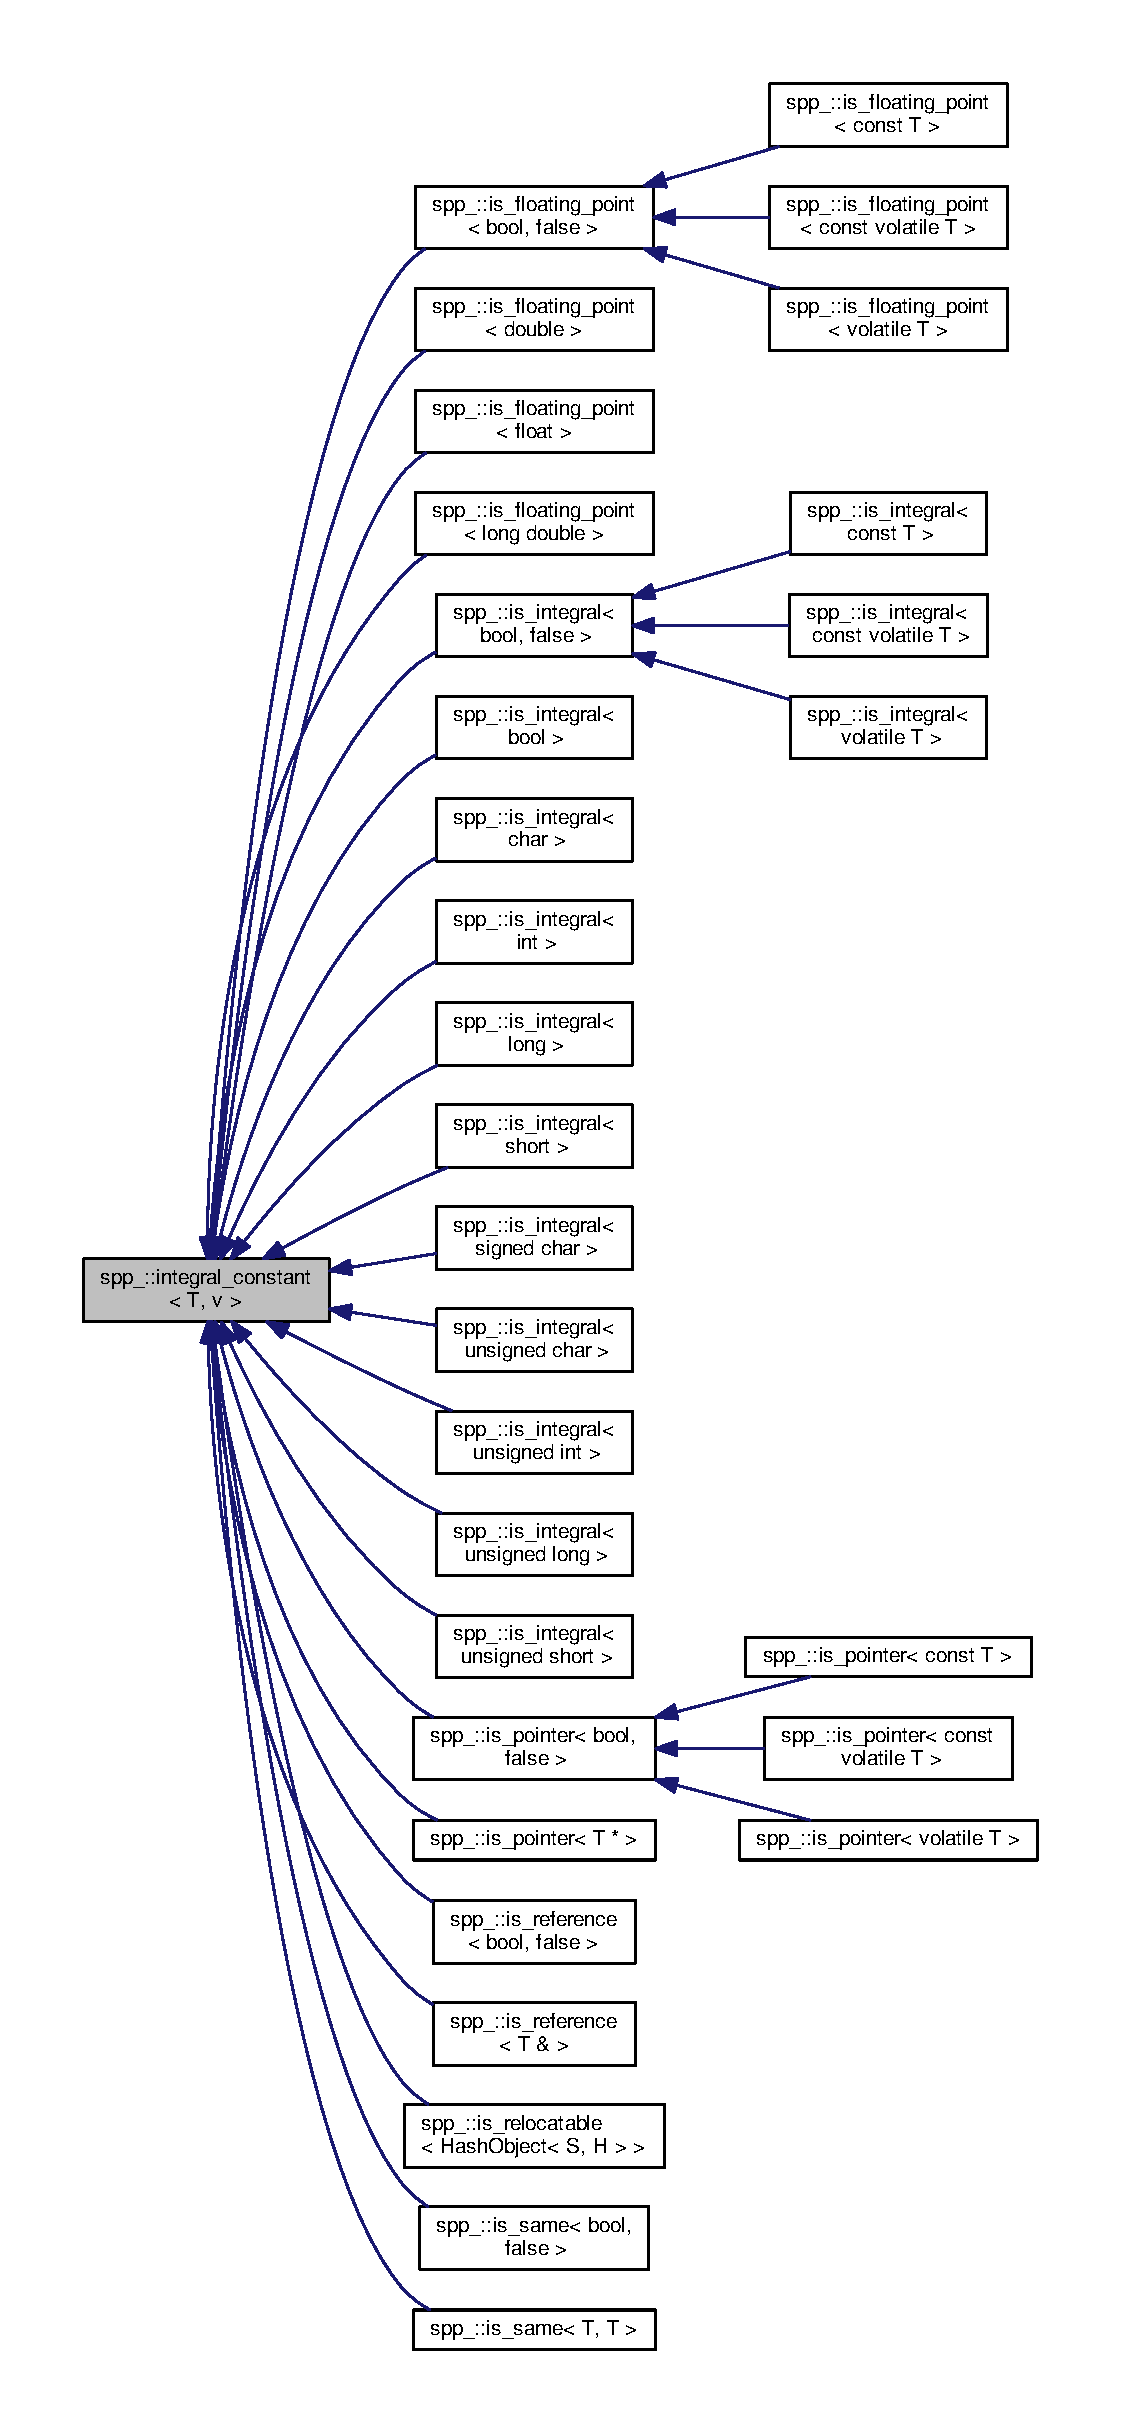
\includegraphics[height=550pt]{structspp___1_1integral__constant__inherit__graph}
\end{center}
\end{figure}


Collaboration diagram for spp\+\_\+\+:\+:integral\+\_\+constant$<$ T, v $>$\+:\nopagebreak
\begin{figure}[H]
\begin{center}
\leavevmode
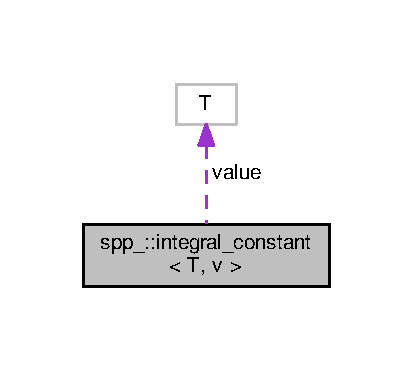
\includegraphics[width=198pt]{structspp___1_1integral__constant__coll__graph}
\end{center}
\end{figure}
\subsection*{Static Public Attributes}
\begin{DoxyCompactItemize}
\item 
static const T {\bfseries value} = v\hypertarget{structspp___1_1integral__constant_a820280bb0a8bdcb52886e4568f46c65d}{}\label{structspp___1_1integral__constant_a820280bb0a8bdcb52886e4568f46c65d}

\end{DoxyCompactItemize}


The documentation for this struct was generated from the following file\+:\begin{DoxyCompactItemize}
\item 
include/sparsepp/spp\+\_\+traits.\+h\end{DoxyCompactItemize}

\hypertarget{classdbt_1_1_interpreter}{}\section{dbt\+:\+:Interpreter Class Reference}
\label{classdbt_1_1_interpreter}\index{dbt\+::\+Interpreter@{dbt\+::\+Interpreter}}


Inheritance diagram for dbt\+:\+:Interpreter\+:\nopagebreak
\begin{figure}[H]
\begin{center}
\leavevmode
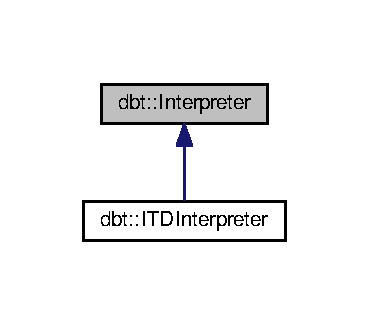
\includegraphics[width=177pt]{classdbt_1_1_interpreter__inherit__graph}
\end{center}
\end{figure}


Collaboration diagram for dbt\+:\+:Interpreter\+:\nopagebreak
\begin{figure}[H]
\begin{center}
\leavevmode
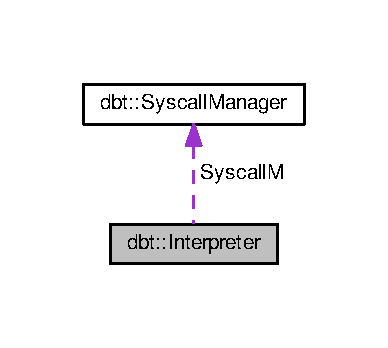
\includegraphics[width=186pt]{classdbt_1_1_interpreter__coll__graph}
\end{center}
\end{figure}
\subsection*{Public Member Functions}
\begin{DoxyCompactItemize}
\item 
{\bfseries Interpreter} (\hyperlink{classdbt_1_1_syscall_manager}{Syscall\+Manager} \&SM)\hypertarget{classdbt_1_1_interpreter_a3d7898f615730fefb25fbccac673907b}{}\label{classdbt_1_1_interpreter_a3d7898f615730fefb25fbccac673907b}

\item 
virtual void {\bfseries execute} (\hyperlink{classdbt_1_1_machine}{Machine} \&, uint32\+\_\+t, uint32\+\_\+t)=0\hypertarget{classdbt_1_1_interpreter_aa660f40fa6b58301c42e499f6a0327c9}{}\label{classdbt_1_1_interpreter_aa660f40fa6b58301c42e499f6a0327c9}

\item 
void {\bfseries execute\+All} (\hyperlink{classdbt_1_1_machine}{Machine} \&M)\hypertarget{classdbt_1_1_interpreter_a5e5fc40019057b107ebfd0b6b8443751}{}\label{classdbt_1_1_interpreter_a5e5fc40019057b107ebfd0b6b8443751}

\end{DoxyCompactItemize}
\subsection*{Protected Attributes}
\begin{DoxyCompactItemize}
\item 
\hyperlink{classdbt_1_1_syscall_manager}{Syscall\+Manager} \& {\bfseries SyscallM}\hypertarget{classdbt_1_1_interpreter_ad9cba79a792cf3b8e7e641ccc3587c2a}{}\label{classdbt_1_1_interpreter_ad9cba79a792cf3b8e7e641ccc3587c2a}

\end{DoxyCompactItemize}


The documentation for this class was generated from the following file\+:\begin{DoxyCompactItemize}
\item 
include/interpreter.\+hpp\end{DoxyCompactItemize}

\hypertarget{classdbt_1_1_i_r_emitter}{}\section{dbt\+:\+:I\+R\+Emitter Class Reference}
\label{classdbt_1_1_i_r_emitter}\index{dbt\+::\+I\+R\+Emitter@{dbt\+::\+I\+R\+Emitter}}
\subsection*{Public Member Functions}
\begin{DoxyCompactItemize}
\item 
std\+::vector$<$ uint32\+\_\+t $>$ {\bfseries get\+Direct\+Transitions} (uint32\+\_\+t Addrs)\hypertarget{classdbt_1_1_i_r_emitter_a5ef6352dfc402795674f6f159035c385}{}\label{classdbt_1_1_i_r_emitter_a5ef6352dfc402795674f6f159035c385}

\item 
llvm\+::\+Module $\ast$ {\bfseries generate\+Region\+IR} (uint32\+\_\+t, const O\+I\+Inst\+List \&, uint32\+\_\+t, spp\+::sparse\+\_\+hash\+\_\+map$<$ uint32\+\_\+t, uint32\+\_\+t $>$ \&, llvm\+::\+Target\+Machine \&, volatile uint64\+\_\+t $\ast$Native\+Regions)\hypertarget{classdbt_1_1_i_r_emitter_aa7ba17ebd138f6d47887b07da68c55bb}{}\label{classdbt_1_1_i_r_emitter_aa7ba17ebd138f6d47887b07da68c55bb}

\item 
llvm\+::\+Module $\ast$ {\bfseries generate\+Merged\+Regions} (std\+::vector$<$ O\+I\+Inst\+List $>$ \&, uint32\+\_\+t, spp\+::sparse\+\_\+hash\+\_\+map$<$ uint32\+\_\+t, uint32\+\_\+t $>$ \&, llvm\+::\+Target\+Machine \&)\hypertarget{classdbt_1_1_i_r_emitter_a3d8a68fc7fb73739ea2de082419e4bf8}{}\label{classdbt_1_1_i_r_emitter_a3d8a68fc7fb73739ea2de082419e4bf8}

\end{DoxyCompactItemize}
\subsection*{Static Public Member Functions}
\begin{DoxyCompactItemize}
\item 
static size\+\_\+t {\bfseries disassemble} (const void $\ast$func, std\+::ostream \&buffer)\hypertarget{classdbt_1_1_i_r_emitter_a90567800f6b634500ab95097ab717aea}{}\label{classdbt_1_1_i_r_emitter_a90567800f6b634500ab95097ab717aea}

\item 
static size\+\_\+t {\bfseries region\+Dump} (const void $\ast$func, std\+::ostream \&buffer, size\+\_\+t size)\hypertarget{classdbt_1_1_i_r_emitter_ae37ff1644a96df74589e490694ee6641}{}\label{classdbt_1_1_i_r_emitter_ae37ff1644a96df74589e490694ee6641}

\end{DoxyCompactItemize}


The documentation for this class was generated from the following files\+:\begin{DoxyCompactItemize}
\item 
include/I\+R\+Emitter.\+hpp\item 
I\+R\+Emitter.\+cpp\item 
I\+R\+Utils.\+cpp\end{DoxyCompactItemize}

\hypertarget{classllvm_1_1orc_1_1_i_r_lazy_j_i_t}{}\section{llvm\+:\+:orc\+:\+:I\+R\+Lazy\+J\+IT Class Reference}
\label{classllvm_1_1orc_1_1_i_r_lazy_j_i_t}\index{llvm\+::orc\+::\+I\+R\+Lazy\+J\+IT@{llvm\+::orc\+::\+I\+R\+Lazy\+J\+IT}}
\subsection*{Public Types}
\begin{DoxyCompactItemize}
\item 
using {\bfseries Obj\+LayerT} = R\+T\+Dyld\+Object\+Linking\+Layer\hypertarget{classllvm_1_1orc_1_1_i_r_lazy_j_i_t_aa38d34dc778643c79ebf32790c85e8bf}{}\label{classllvm_1_1orc_1_1_i_r_lazy_j_i_t_aa38d34dc778643c79ebf32790c85e8bf}

\item 
using {\bfseries Compile\+LayerT} = I\+R\+Compile\+Layer$<$ Obj\+LayerT, Simple\+Compiler $>$\hypertarget{classllvm_1_1orc_1_1_i_r_lazy_j_i_t_a6295103c3e813290d1359ec7d5771b27}{}\label{classllvm_1_1orc_1_1_i_r_lazy_j_i_t_a6295103c3e813290d1359ec7d5771b27}

\item 
using {\bfseries Module\+HandleT} = Compile\+Layer\+T\+::\+Module\+HandleT\hypertarget{classllvm_1_1orc_1_1_i_r_lazy_j_i_t_ab48ef40ded83ea0117c98b55cf93712e}{}\label{classllvm_1_1orc_1_1_i_r_lazy_j_i_t_ab48ef40ded83ea0117c98b55cf93712e}

\end{DoxyCompactItemize}
\subsection*{Public Member Functions}
\begin{DoxyCompactItemize}
\item 
Target\+Machine \& {\bfseries get\+Target\+Machine} ()\hypertarget{classllvm_1_1orc_1_1_i_r_lazy_j_i_t_a01f3adde0081fb2ab00ef823e8c1712f}{}\label{classllvm_1_1orc_1_1_i_r_lazy_j_i_t_a01f3adde0081fb2ab00ef823e8c1712f}

\item 
Module\+HandleT {\bfseries add\+Module} (std\+::unique\+\_\+ptr$<$ Module $>$ M)\hypertarget{classllvm_1_1orc_1_1_i_r_lazy_j_i_t_a98746df5165ebcf5d2358e275cbbb4ef}{}\label{classllvm_1_1orc_1_1_i_r_lazy_j_i_t_a98746df5165ebcf5d2358e275cbbb4ef}

\item 
void {\bfseries remove\+Module} (Module\+HandleT H)\hypertarget{classllvm_1_1orc_1_1_i_r_lazy_j_i_t_affd00d53768bd9b50e1e68521d4d1aca}{}\label{classllvm_1_1orc_1_1_i_r_lazy_j_i_t_affd00d53768bd9b50e1e68521d4d1aca}

\item 
J\+I\+T\+Symbol {\bfseries find\+Symbol} (const std\+::string Name)\hypertarget{classllvm_1_1orc_1_1_i_r_lazy_j_i_t_a251720f0ec33b902836990c74143cd02}{}\label{classllvm_1_1orc_1_1_i_r_lazy_j_i_t_a251720f0ec33b902836990c74143cd02}

\end{DoxyCompactItemize}


The documentation for this class was generated from the following file\+:\begin{DoxyCompactItemize}
\item 
include/I\+R\+Lazy\+J\+I\+T.\+hpp\end{DoxyCompactItemize}

\hypertarget{classdbt_1_1_i_r_opt}{}\section{dbt\+:\+:I\+R\+Opt Class Reference}
\label{classdbt_1_1_i_r_opt}\index{dbt\+::\+I\+R\+Opt@{dbt\+::\+I\+R\+Opt}}
\subsection*{Public Types}
\begin{DoxyCompactItemize}
\item 
enum {\bfseries Opt\+Level} \{ {\bfseries Basic}, 
{\bfseries Soft}, 
{\bfseries Medium}, 
{\bfseries Hard}
 \}\hypertarget{classdbt_1_1_i_r_opt_a269a9377acf828ee812af3c98295e235}{}\label{classdbt_1_1_i_r_opt_a269a9377acf828ee812af3c98295e235}

\end{DoxyCompactItemize}
\subsection*{Public Member Functions}
\begin{DoxyCompactItemize}
\item 
void {\bfseries optimize\+I\+R\+Function} (llvm\+::\+Module $\ast$, Opt\+Level)\hypertarget{classdbt_1_1_i_r_opt_a143ef63180958877aacc34698cb30cb6}{}\label{classdbt_1_1_i_r_opt_a143ef63180958877aacc34698cb30cb6}

\end{DoxyCompactItemize}


The documentation for this class was generated from the following files\+:\begin{DoxyCompactItemize}
\item 
include/I\+R\+Opt.\+hpp\item 
I\+R\+Opt.\+cpp\end{DoxyCompactItemize}

\hypertarget{structspp___1_1is__floating__point}{}\section{spp\+\_\+\+:\+:is\+\_\+floating\+\_\+point$<$ T $>$ Struct Template Reference}
\label{structspp___1_1is__floating__point}\index{spp\+\_\+\+::is\+\_\+floating\+\_\+point$<$ T $>$@{spp\+\_\+\+::is\+\_\+floating\+\_\+point$<$ T $>$}}


Inheritance diagram for spp\+\_\+\+:\+:is\+\_\+floating\+\_\+point$<$ T $>$\+:\nopagebreak
\begin{figure}[H]
\begin{center}
\leavevmode
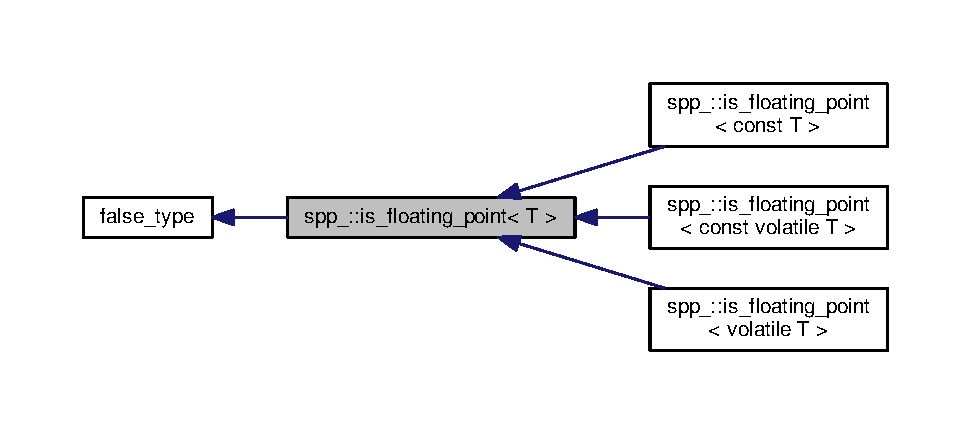
\includegraphics[width=350pt]{structspp___1_1is__floating__point__inherit__graph}
\end{center}
\end{figure}


Collaboration diagram for spp\+\_\+\+:\+:is\+\_\+floating\+\_\+point$<$ T $>$\+:\nopagebreak
\begin{figure}[H]
\begin{center}
\leavevmode
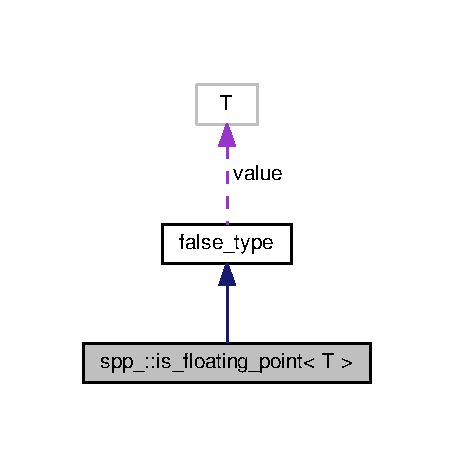
\includegraphics[width=218pt]{structspp___1_1is__floating__point__coll__graph}
\end{center}
\end{figure}
\subsection*{Additional Inherited Members}


The documentation for this struct was generated from the following file\+:\begin{DoxyCompactItemize}
\item 
include/sparsepp/spp\+\_\+traits.\+h\end{DoxyCompactItemize}

\hypertarget{structspp___1_1is__floating__point_3_01const_01_t_01_4}{}\section{spp\+\_\+\+:\+:is\+\_\+floating\+\_\+point$<$ const T $>$ Struct Template Reference}
\label{structspp___1_1is__floating__point_3_01const_01_t_01_4}\index{spp\+\_\+\+::is\+\_\+floating\+\_\+point$<$ const T $>$@{spp\+\_\+\+::is\+\_\+floating\+\_\+point$<$ const T $>$}}


Inheritance diagram for spp\+\_\+\+:\+:is\+\_\+floating\+\_\+point$<$ const T $>$\+:\nopagebreak
\begin{figure}[H]
\begin{center}
\leavevmode
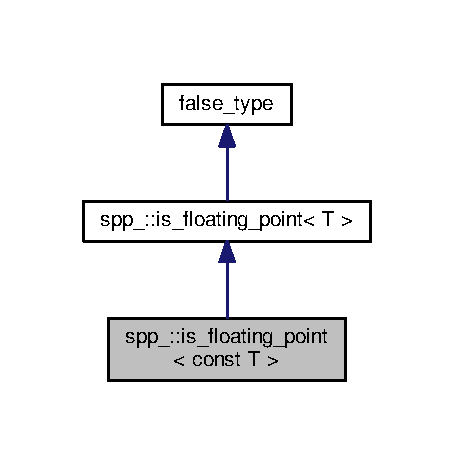
\includegraphics[width=218pt]{structspp___1_1is__floating__point_3_01const_01_t_01_4__inherit__graph}
\end{center}
\end{figure}


Collaboration diagram for spp\+\_\+\+:\+:is\+\_\+floating\+\_\+point$<$ const T $>$\+:\nopagebreak
\begin{figure}[H]
\begin{center}
\leavevmode
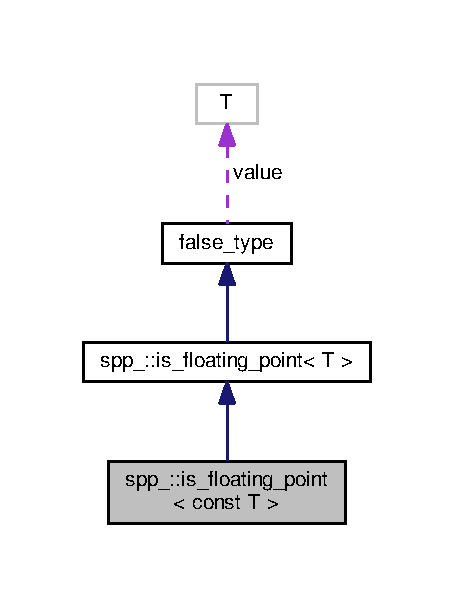
\includegraphics[width=218pt]{structspp___1_1is__floating__point_3_01const_01_t_01_4__coll__graph}
\end{center}
\end{figure}
\subsection*{Additional Inherited Members}


The documentation for this struct was generated from the following file\+:\begin{DoxyCompactItemize}
\item 
include/sparsepp/spp\+\_\+traits.\+h\end{DoxyCompactItemize}

\hypertarget{structspp___1_1is__floating__point_3_01const_01volatile_01_t_01_4}{}\section{spp\+\_\+\+:\+:is\+\_\+floating\+\_\+point$<$ const volatile T $>$ Struct Template Reference}
\label{structspp___1_1is__floating__point_3_01const_01volatile_01_t_01_4}\index{spp\+\_\+\+::is\+\_\+floating\+\_\+point$<$ const volatile T $>$@{spp\+\_\+\+::is\+\_\+floating\+\_\+point$<$ const volatile T $>$}}


Inheritance diagram for spp\+\_\+\+:\+:is\+\_\+floating\+\_\+point$<$ const volatile T $>$\+:\nopagebreak
\begin{figure}[H]
\begin{center}
\leavevmode
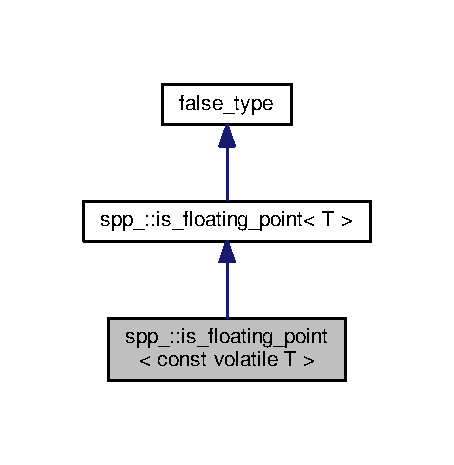
\includegraphics[width=218pt]{structspp___1_1is__floating__point_3_01const_01volatile_01_t_01_4__inherit__graph}
\end{center}
\end{figure}


Collaboration diagram for spp\+\_\+\+:\+:is\+\_\+floating\+\_\+point$<$ const volatile T $>$\+:\nopagebreak
\begin{figure}[H]
\begin{center}
\leavevmode
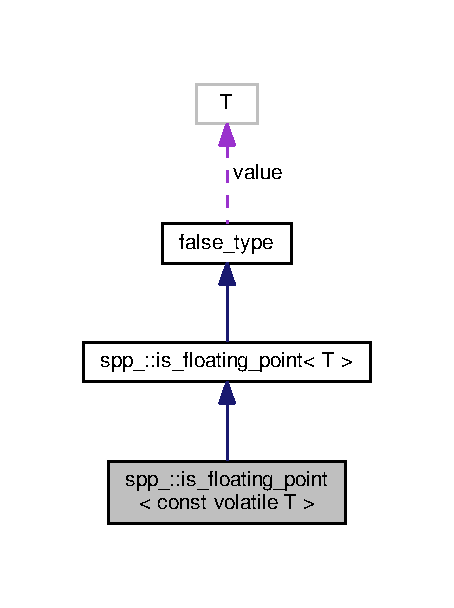
\includegraphics[width=218pt]{structspp___1_1is__floating__point_3_01const_01volatile_01_t_01_4__coll__graph}
\end{center}
\end{figure}
\subsection*{Additional Inherited Members}


The documentation for this struct was generated from the following file\+:\begin{DoxyCompactItemize}
\item 
include/sparsepp/spp\+\_\+traits.\+h\end{DoxyCompactItemize}

\hypertarget{structspp___1_1is__floating__point_3_01double_01_4}{}\section{spp\+\_\+\+:\+:is\+\_\+floating\+\_\+point$<$ double $>$ Struct Template Reference}
\label{structspp___1_1is__floating__point_3_01double_01_4}\index{spp\+\_\+\+::is\+\_\+floating\+\_\+point$<$ double $>$@{spp\+\_\+\+::is\+\_\+floating\+\_\+point$<$ double $>$}}


Inheritance diagram for spp\+\_\+\+:\+:is\+\_\+floating\+\_\+point$<$ double $>$\+:\nopagebreak
\begin{figure}[H]
\begin{center}
\leavevmode
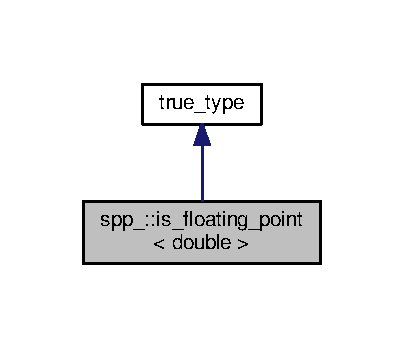
\includegraphics[width=194pt]{structspp___1_1is__floating__point_3_01double_01_4__inherit__graph}
\end{center}
\end{figure}


Collaboration diagram for spp\+\_\+\+:\+:is\+\_\+floating\+\_\+point$<$ double $>$\+:\nopagebreak
\begin{figure}[H]
\begin{center}
\leavevmode
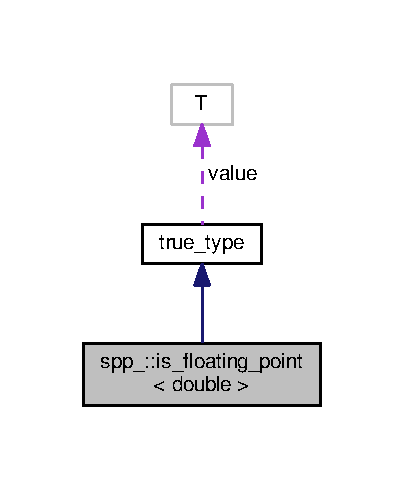
\includegraphics[width=194pt]{structspp___1_1is__floating__point_3_01double_01_4__coll__graph}
\end{center}
\end{figure}
\subsection*{Additional Inherited Members}


The documentation for this struct was generated from the following file\+:\begin{DoxyCompactItemize}
\item 
include/sparsepp/spp\+\_\+traits.\+h\end{DoxyCompactItemize}

\hypertarget{structspp___1_1is__floating__point_3_01float_01_4}{}\section{spp\+\_\+\+:\+:is\+\_\+floating\+\_\+point$<$ float $>$ Struct Template Reference}
\label{structspp___1_1is__floating__point_3_01float_01_4}\index{spp\+\_\+\+::is\+\_\+floating\+\_\+point$<$ float $>$@{spp\+\_\+\+::is\+\_\+floating\+\_\+point$<$ float $>$}}


Inheritance diagram for spp\+\_\+\+:\+:is\+\_\+floating\+\_\+point$<$ float $>$\+:\nopagebreak
\begin{figure}[H]
\begin{center}
\leavevmode
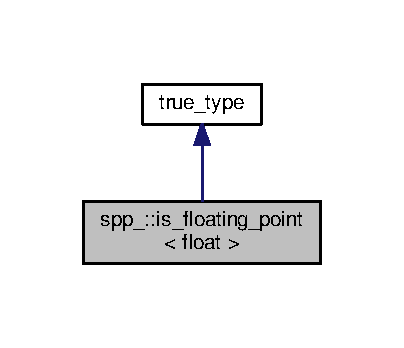
\includegraphics[width=194pt]{structspp___1_1is__floating__point_3_01float_01_4__inherit__graph}
\end{center}
\end{figure}


Collaboration diagram for spp\+\_\+\+:\+:is\+\_\+floating\+\_\+point$<$ float $>$\+:\nopagebreak
\begin{figure}[H]
\begin{center}
\leavevmode
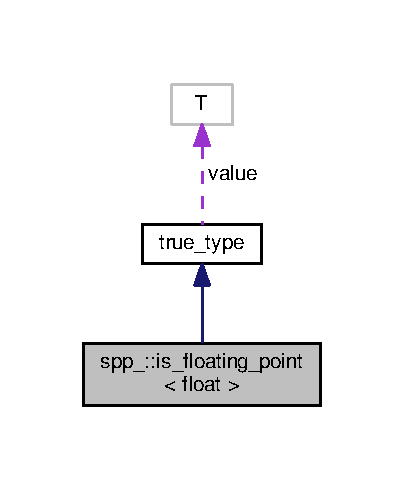
\includegraphics[width=194pt]{structspp___1_1is__floating__point_3_01float_01_4__coll__graph}
\end{center}
\end{figure}
\subsection*{Additional Inherited Members}


The documentation for this struct was generated from the following file\+:\begin{DoxyCompactItemize}
\item 
include/sparsepp/spp\+\_\+traits.\+h\end{DoxyCompactItemize}

\hypertarget{structspp___1_1is__floating__point_3_01long_01double_01_4}{}\section{spp\+\_\+\+:\+:is\+\_\+floating\+\_\+point$<$ long double $>$ Struct Template Reference}
\label{structspp___1_1is__floating__point_3_01long_01double_01_4}\index{spp\+\_\+\+::is\+\_\+floating\+\_\+point$<$ long double $>$@{spp\+\_\+\+::is\+\_\+floating\+\_\+point$<$ long double $>$}}


Inheritance diagram for spp\+\_\+\+:\+:is\+\_\+floating\+\_\+point$<$ long double $>$\+:\nopagebreak
\begin{figure}[H]
\begin{center}
\leavevmode
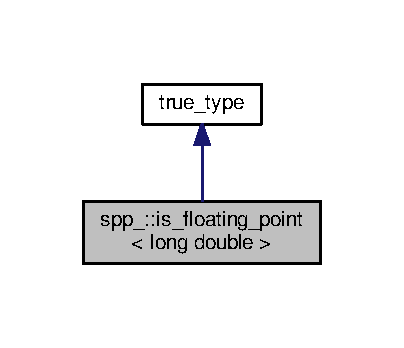
\includegraphics[width=194pt]{structspp___1_1is__floating__point_3_01long_01double_01_4__inherit__graph}
\end{center}
\end{figure}


Collaboration diagram for spp\+\_\+\+:\+:is\+\_\+floating\+\_\+point$<$ long double $>$\+:\nopagebreak
\begin{figure}[H]
\begin{center}
\leavevmode
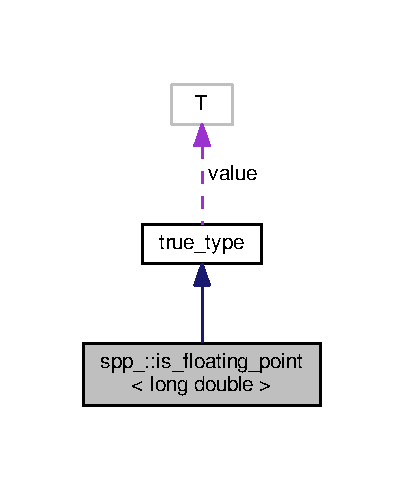
\includegraphics[width=194pt]{structspp___1_1is__floating__point_3_01long_01double_01_4__coll__graph}
\end{center}
\end{figure}
\subsection*{Additional Inherited Members}


The documentation for this struct was generated from the following file\+:\begin{DoxyCompactItemize}
\item 
include/sparsepp/spp\+\_\+traits.\+h\end{DoxyCompactItemize}

\hypertarget{structspp___1_1is__floating__point_3_01volatile_01_t_01_4}{}\section{spp\+\_\+\+:\+:is\+\_\+floating\+\_\+point$<$ volatile T $>$ Struct Template Reference}
\label{structspp___1_1is__floating__point_3_01volatile_01_t_01_4}\index{spp\+\_\+\+::is\+\_\+floating\+\_\+point$<$ volatile T $>$@{spp\+\_\+\+::is\+\_\+floating\+\_\+point$<$ volatile T $>$}}


Inheritance diagram for spp\+\_\+\+:\+:is\+\_\+floating\+\_\+point$<$ volatile T $>$\+:\nopagebreak
\begin{figure}[H]
\begin{center}
\leavevmode
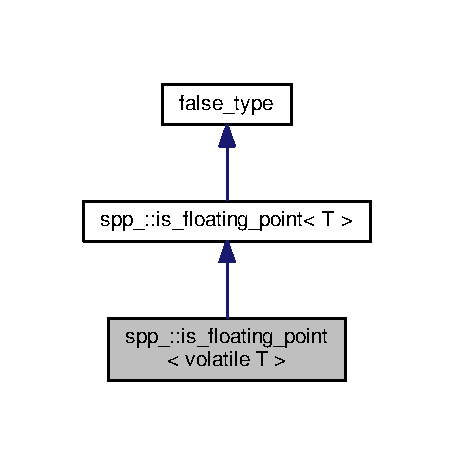
\includegraphics[width=218pt]{structspp___1_1is__floating__point_3_01volatile_01_t_01_4__inherit__graph}
\end{center}
\end{figure}


Collaboration diagram for spp\+\_\+\+:\+:is\+\_\+floating\+\_\+point$<$ volatile T $>$\+:\nopagebreak
\begin{figure}[H]
\begin{center}
\leavevmode
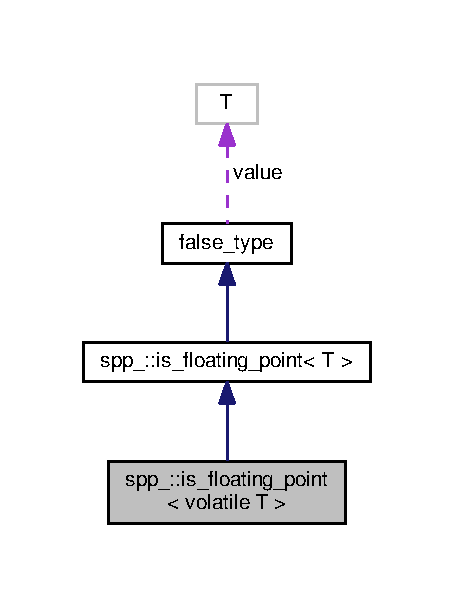
\includegraphics[width=218pt]{structspp___1_1is__floating__point_3_01volatile_01_t_01_4__coll__graph}
\end{center}
\end{figure}
\subsection*{Additional Inherited Members}


The documentation for this struct was generated from the following file\+:\begin{DoxyCompactItemize}
\item 
include/sparsepp/spp\+\_\+traits.\+h\end{DoxyCompactItemize}

\hypertarget{structspp___1_1is__integral}{}\section{spp\+\_\+\+:\+:is\+\_\+integral$<$ T $>$ Struct Template Reference}
\label{structspp___1_1is__integral}\index{spp\+\_\+\+::is\+\_\+integral$<$ T $>$@{spp\+\_\+\+::is\+\_\+integral$<$ T $>$}}


Inheritance diagram for spp\+\_\+\+:\+:is\+\_\+integral$<$ T $>$\+:\nopagebreak
\begin{figure}[H]
\begin{center}
\leavevmode
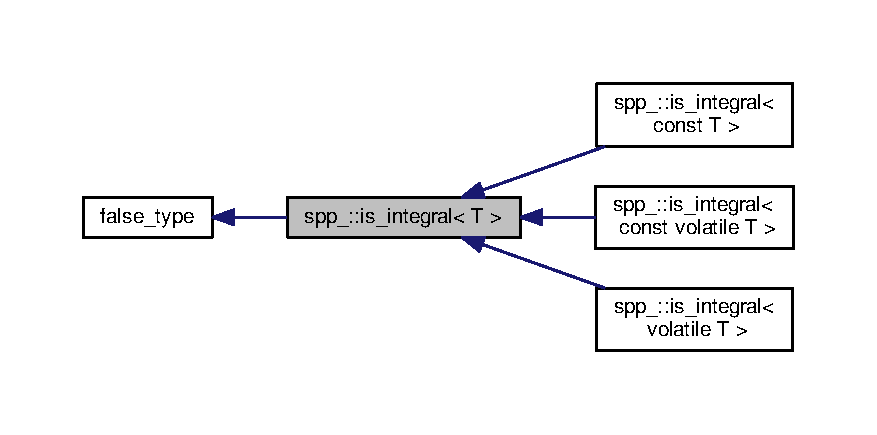
\includegraphics[width=350pt]{structspp___1_1is__integral__inherit__graph}
\end{center}
\end{figure}


Collaboration diagram for spp\+\_\+\+:\+:is\+\_\+integral$<$ T $>$\+:\nopagebreak
\begin{figure}[H]
\begin{center}
\leavevmode
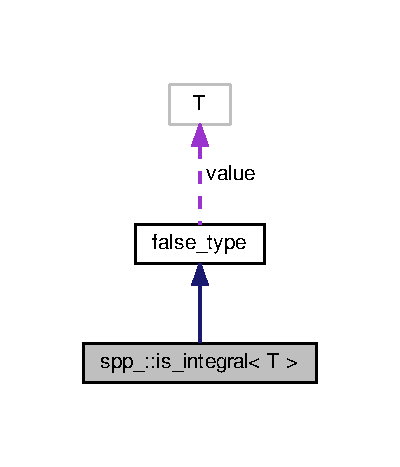
\includegraphics[width=192pt]{structspp___1_1is__integral__coll__graph}
\end{center}
\end{figure}
\subsection*{Additional Inherited Members}


The documentation for this struct was generated from the following file\+:\begin{DoxyCompactItemize}
\item 
include/sparsepp/spp\+\_\+traits.\+h\end{DoxyCompactItemize}

\hypertarget{structspp___1_1is__integral_3_01bool_01_4}{}\section{spp\+\_\+\+:\+:is\+\_\+integral$<$ bool $>$ Struct Template Reference}
\label{structspp___1_1is__integral_3_01bool_01_4}\index{spp\+\_\+\+::is\+\_\+integral$<$ bool $>$@{spp\+\_\+\+::is\+\_\+integral$<$ bool $>$}}


Inheritance diagram for spp\+\_\+\+:\+:is\+\_\+integral$<$ bool $>$\+:\nopagebreak
\begin{figure}[H]
\begin{center}
\leavevmode
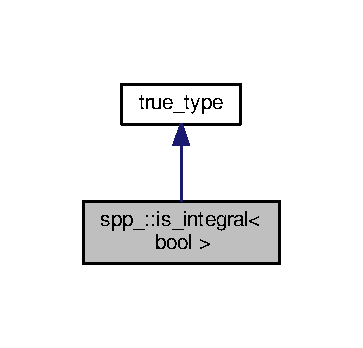
\includegraphics[width=174pt]{structspp___1_1is__integral_3_01bool_01_4__inherit__graph}
\end{center}
\end{figure}


Collaboration diagram for spp\+\_\+\+:\+:is\+\_\+integral$<$ bool $>$\+:\nopagebreak
\begin{figure}[H]
\begin{center}
\leavevmode
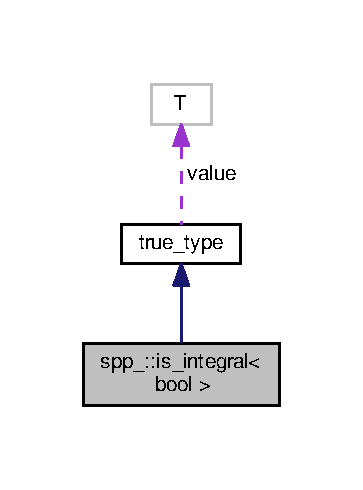
\includegraphics[width=174pt]{structspp___1_1is__integral_3_01bool_01_4__coll__graph}
\end{center}
\end{figure}
\subsection*{Additional Inherited Members}


The documentation for this struct was generated from the following file\+:\begin{DoxyCompactItemize}
\item 
include/sparsepp/spp\+\_\+traits.\+h\end{DoxyCompactItemize}

\hypertarget{structspp___1_1is__integral_3_01char_01_4}{}\section{spp\+\_\+\+:\+:is\+\_\+integral$<$ char $>$ Struct Template Reference}
\label{structspp___1_1is__integral_3_01char_01_4}\index{spp\+\_\+\+::is\+\_\+integral$<$ char $>$@{spp\+\_\+\+::is\+\_\+integral$<$ char $>$}}


Inheritance diagram for spp\+\_\+\+:\+:is\+\_\+integral$<$ char $>$\+:\nopagebreak
\begin{figure}[H]
\begin{center}
\leavevmode
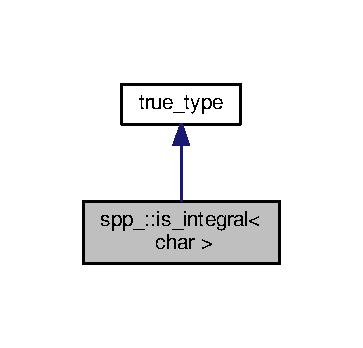
\includegraphics[width=174pt]{structspp___1_1is__integral_3_01char_01_4__inherit__graph}
\end{center}
\end{figure}


Collaboration diagram for spp\+\_\+\+:\+:is\+\_\+integral$<$ char $>$\+:\nopagebreak
\begin{figure}[H]
\begin{center}
\leavevmode
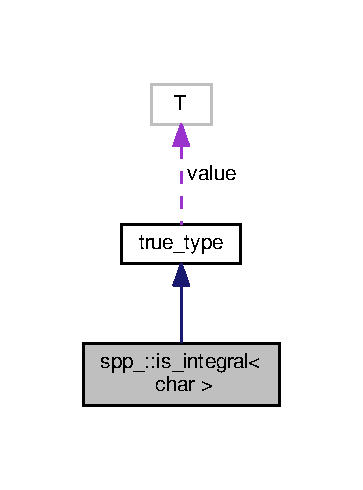
\includegraphics[width=174pt]{structspp___1_1is__integral_3_01char_01_4__coll__graph}
\end{center}
\end{figure}
\subsection*{Additional Inherited Members}


The documentation for this struct was generated from the following file\+:\begin{DoxyCompactItemize}
\item 
include/sparsepp/spp\+\_\+traits.\+h\end{DoxyCompactItemize}

\hypertarget{structspp___1_1is__integral_3_01const_01_t_01_4}{}\section{spp\+\_\+\+:\+:is\+\_\+integral$<$ const T $>$ Struct Template Reference}
\label{structspp___1_1is__integral_3_01const_01_t_01_4}\index{spp\+\_\+\+::is\+\_\+integral$<$ const T $>$@{spp\+\_\+\+::is\+\_\+integral$<$ const T $>$}}


Inheritance diagram for spp\+\_\+\+:\+:is\+\_\+integral$<$ const T $>$\+:\nopagebreak
\begin{figure}[H]
\begin{center}
\leavevmode
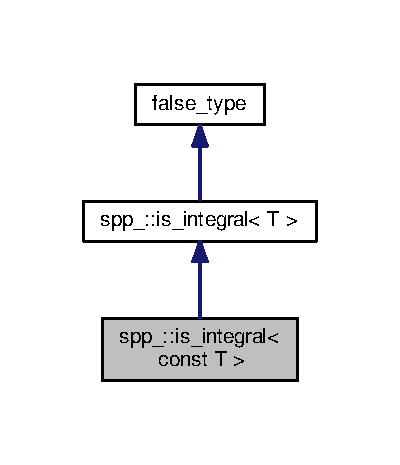
\includegraphics[width=192pt]{structspp___1_1is__integral_3_01const_01_t_01_4__inherit__graph}
\end{center}
\end{figure}


Collaboration diagram for spp\+\_\+\+:\+:is\+\_\+integral$<$ const T $>$\+:\nopagebreak
\begin{figure}[H]
\begin{center}
\leavevmode
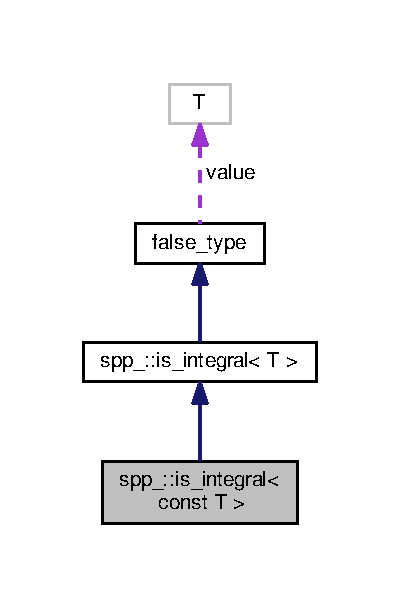
\includegraphics[width=192pt]{structspp___1_1is__integral_3_01const_01_t_01_4__coll__graph}
\end{center}
\end{figure}
\subsection*{Additional Inherited Members}


The documentation for this struct was generated from the following file\+:\begin{DoxyCompactItemize}
\item 
include/sparsepp/spp\+\_\+traits.\+h\end{DoxyCompactItemize}

\hypertarget{structspp___1_1is__integral_3_01const_01volatile_01_t_01_4}{}\section{spp\+\_\+\+:\+:is\+\_\+integral$<$ const volatile T $>$ Struct Template Reference}
\label{structspp___1_1is__integral_3_01const_01volatile_01_t_01_4}\index{spp\+\_\+\+::is\+\_\+integral$<$ const volatile T $>$@{spp\+\_\+\+::is\+\_\+integral$<$ const volatile T $>$}}


Inheritance diagram for spp\+\_\+\+:\+:is\+\_\+integral$<$ const volatile T $>$\+:\nopagebreak
\begin{figure}[H]
\begin{center}
\leavevmode
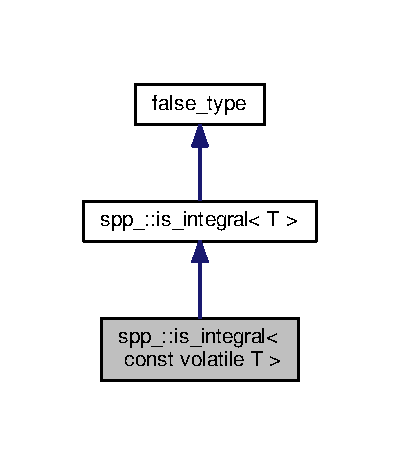
\includegraphics[width=192pt]{structspp___1_1is__integral_3_01const_01volatile_01_t_01_4__inherit__graph}
\end{center}
\end{figure}


Collaboration diagram for spp\+\_\+\+:\+:is\+\_\+integral$<$ const volatile T $>$\+:\nopagebreak
\begin{figure}[H]
\begin{center}
\leavevmode
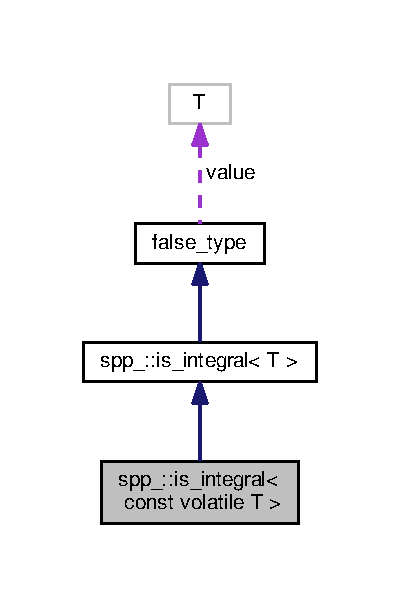
\includegraphics[width=192pt]{structspp___1_1is__integral_3_01const_01volatile_01_t_01_4__coll__graph}
\end{center}
\end{figure}
\subsection*{Additional Inherited Members}


The documentation for this struct was generated from the following file\+:\begin{DoxyCompactItemize}
\item 
include/sparsepp/spp\+\_\+traits.\+h\end{DoxyCompactItemize}

\hypertarget{structspp___1_1is__integral_3_01int_01_4}{}\section{spp\+\_\+\+:\+:is\+\_\+integral$<$ int $>$ Struct Template Reference}
\label{structspp___1_1is__integral_3_01int_01_4}\index{spp\+\_\+\+::is\+\_\+integral$<$ int $>$@{spp\+\_\+\+::is\+\_\+integral$<$ int $>$}}


Inheritance diagram for spp\+\_\+\+:\+:is\+\_\+integral$<$ int $>$\+:\nopagebreak
\begin{figure}[H]
\begin{center}
\leavevmode
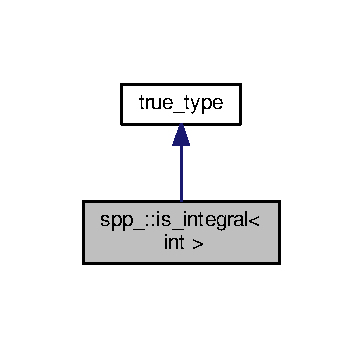
\includegraphics[width=174pt]{structspp___1_1is__integral_3_01int_01_4__inherit__graph}
\end{center}
\end{figure}


Collaboration diagram for spp\+\_\+\+:\+:is\+\_\+integral$<$ int $>$\+:\nopagebreak
\begin{figure}[H]
\begin{center}
\leavevmode
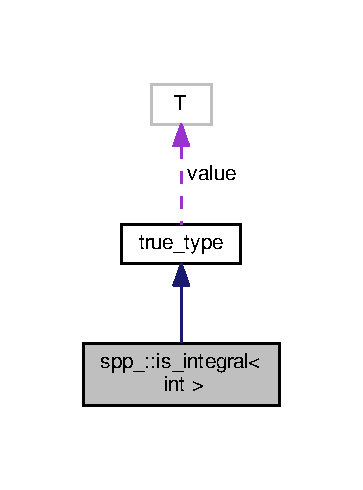
\includegraphics[width=174pt]{structspp___1_1is__integral_3_01int_01_4__coll__graph}
\end{center}
\end{figure}
\subsection*{Additional Inherited Members}


The documentation for this struct was generated from the following file\+:\begin{DoxyCompactItemize}
\item 
include/sparsepp/spp\+\_\+traits.\+h\end{DoxyCompactItemize}

\hypertarget{structspp___1_1is__integral_3_01long_01_4}{}\section{spp\+\_\+\+:\+:is\+\_\+integral$<$ long $>$ Struct Template Reference}
\label{structspp___1_1is__integral_3_01long_01_4}\index{spp\+\_\+\+::is\+\_\+integral$<$ long $>$@{spp\+\_\+\+::is\+\_\+integral$<$ long $>$}}


Inheritance diagram for spp\+\_\+\+:\+:is\+\_\+integral$<$ long $>$\+:\nopagebreak
\begin{figure}[H]
\begin{center}
\leavevmode
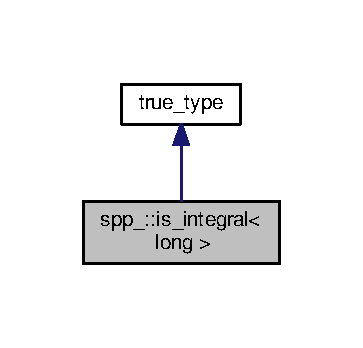
\includegraphics[width=174pt]{structspp___1_1is__integral_3_01long_01_4__inherit__graph}
\end{center}
\end{figure}


Collaboration diagram for spp\+\_\+\+:\+:is\+\_\+integral$<$ long $>$\+:\nopagebreak
\begin{figure}[H]
\begin{center}
\leavevmode
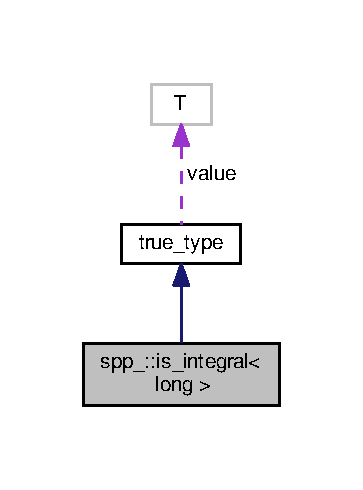
\includegraphics[width=174pt]{structspp___1_1is__integral_3_01long_01_4__coll__graph}
\end{center}
\end{figure}
\subsection*{Additional Inherited Members}


The documentation for this struct was generated from the following file\+:\begin{DoxyCompactItemize}
\item 
include/sparsepp/spp\+\_\+traits.\+h\end{DoxyCompactItemize}

\hypertarget{structspp___1_1is__integral_3_01short_01_4}{}\section{spp\+\_\+\+:\+:is\+\_\+integral$<$ short $>$ Struct Template Reference}
\label{structspp___1_1is__integral_3_01short_01_4}\index{spp\+\_\+\+::is\+\_\+integral$<$ short $>$@{spp\+\_\+\+::is\+\_\+integral$<$ short $>$}}


Inheritance diagram for spp\+\_\+\+:\+:is\+\_\+integral$<$ short $>$\+:\nopagebreak
\begin{figure}[H]
\begin{center}
\leavevmode
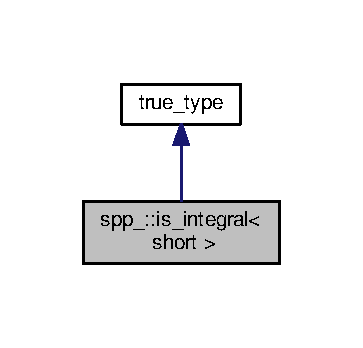
\includegraphics[width=174pt]{structspp___1_1is__integral_3_01short_01_4__inherit__graph}
\end{center}
\end{figure}


Collaboration diagram for spp\+\_\+\+:\+:is\+\_\+integral$<$ short $>$\+:\nopagebreak
\begin{figure}[H]
\begin{center}
\leavevmode
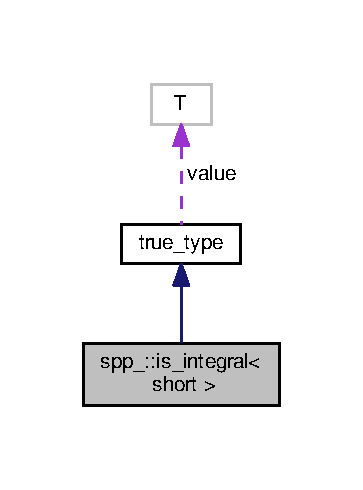
\includegraphics[width=174pt]{structspp___1_1is__integral_3_01short_01_4__coll__graph}
\end{center}
\end{figure}
\subsection*{Additional Inherited Members}


The documentation for this struct was generated from the following file\+:\begin{DoxyCompactItemize}
\item 
include/sparsepp/spp\+\_\+traits.\+h\end{DoxyCompactItemize}

\hypertarget{structspp___1_1is__integral_3_01signed_01char_01_4}{}\section{spp\+\_\+\+:\+:is\+\_\+integral$<$ signed char $>$ Struct Template Reference}
\label{structspp___1_1is__integral_3_01signed_01char_01_4}\index{spp\+\_\+\+::is\+\_\+integral$<$ signed char $>$@{spp\+\_\+\+::is\+\_\+integral$<$ signed char $>$}}


Inheritance diagram for spp\+\_\+\+:\+:is\+\_\+integral$<$ signed char $>$\+:\nopagebreak
\begin{figure}[H]
\begin{center}
\leavevmode
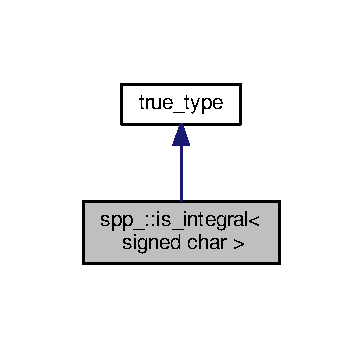
\includegraphics[width=174pt]{structspp___1_1is__integral_3_01signed_01char_01_4__inherit__graph}
\end{center}
\end{figure}


Collaboration diagram for spp\+\_\+\+:\+:is\+\_\+integral$<$ signed char $>$\+:\nopagebreak
\begin{figure}[H]
\begin{center}
\leavevmode
\includegraphics[width=174pt]{structspp___1_1is__integral_3_01signed_01char_01_4__coll__graph}
\end{center}
\end{figure}
\subsection*{Additional Inherited Members}


The documentation for this struct was generated from the following file\+:\begin{DoxyCompactItemize}
\item 
include/sparsepp/spp\+\_\+traits.\+h\end{DoxyCompactItemize}

\hypertarget{structspp___1_1is__integral_3_01unsigned_01char_01_4}{}\section{spp\+\_\+\+:\+:is\+\_\+integral$<$ unsigned char $>$ Struct Template Reference}
\label{structspp___1_1is__integral_3_01unsigned_01char_01_4}\index{spp\+\_\+\+::is\+\_\+integral$<$ unsigned char $>$@{spp\+\_\+\+::is\+\_\+integral$<$ unsigned char $>$}}


Inheritance diagram for spp\+\_\+\+:\+:is\+\_\+integral$<$ unsigned char $>$\+:\nopagebreak
\begin{figure}[H]
\begin{center}
\leavevmode
\includegraphics[width=174pt]{structspp___1_1is__integral_3_01unsigned_01char_01_4__inherit__graph}
\end{center}
\end{figure}


Collaboration diagram for spp\+\_\+\+:\+:is\+\_\+integral$<$ unsigned char $>$\+:\nopagebreak
\begin{figure}[H]
\begin{center}
\leavevmode
\includegraphics[width=174pt]{structspp___1_1is__integral_3_01unsigned_01char_01_4__coll__graph}
\end{center}
\end{figure}
\subsection*{Additional Inherited Members}


The documentation for this struct was generated from the following file\+:\begin{DoxyCompactItemize}
\item 
include/sparsepp/spp\+\_\+traits.\+h\end{DoxyCompactItemize}

\hypertarget{structspp___1_1is__integral_3_01unsigned_01int_01_4}{}\section{spp\+\_\+\+:\+:is\+\_\+integral$<$ unsigned int $>$ Struct Template Reference}
\label{structspp___1_1is__integral_3_01unsigned_01int_01_4}\index{spp\+\_\+\+::is\+\_\+integral$<$ unsigned int $>$@{spp\+\_\+\+::is\+\_\+integral$<$ unsigned int $>$}}


Inheritance diagram for spp\+\_\+\+:\+:is\+\_\+integral$<$ unsigned int $>$\+:\nopagebreak
\begin{figure}[H]
\begin{center}
\leavevmode
\includegraphics[width=174pt]{structspp___1_1is__integral_3_01unsigned_01int_01_4__inherit__graph}
\end{center}
\end{figure}


Collaboration diagram for spp\+\_\+\+:\+:is\+\_\+integral$<$ unsigned int $>$\+:\nopagebreak
\begin{figure}[H]
\begin{center}
\leavevmode
\includegraphics[width=174pt]{structspp___1_1is__integral_3_01unsigned_01int_01_4__coll__graph}
\end{center}
\end{figure}
\subsection*{Additional Inherited Members}


The documentation for this struct was generated from the following file\+:\begin{DoxyCompactItemize}
\item 
include/sparsepp/spp\+\_\+traits.\+h\end{DoxyCompactItemize}

\hypertarget{structspp___1_1is__integral_3_01unsigned_01long_01_4}{}\section{spp\+\_\+\+:\+:is\+\_\+integral$<$ unsigned long $>$ Struct Template Reference}
\label{structspp___1_1is__integral_3_01unsigned_01long_01_4}\index{spp\+\_\+\+::is\+\_\+integral$<$ unsigned long $>$@{spp\+\_\+\+::is\+\_\+integral$<$ unsigned long $>$}}


Inheritance diagram for spp\+\_\+\+:\+:is\+\_\+integral$<$ unsigned long $>$\+:\nopagebreak
\begin{figure}[H]
\begin{center}
\leavevmode
\includegraphics[width=174pt]{structspp___1_1is__integral_3_01unsigned_01long_01_4__inherit__graph}
\end{center}
\end{figure}


Collaboration diagram for spp\+\_\+\+:\+:is\+\_\+integral$<$ unsigned long $>$\+:\nopagebreak
\begin{figure}[H]
\begin{center}
\leavevmode
\includegraphics[width=174pt]{structspp___1_1is__integral_3_01unsigned_01long_01_4__coll__graph}
\end{center}
\end{figure}
\subsection*{Additional Inherited Members}


The documentation for this struct was generated from the following file\+:\begin{DoxyCompactItemize}
\item 
include/sparsepp/spp\+\_\+traits.\+h\end{DoxyCompactItemize}

\hypertarget{structspp___1_1is__integral_3_01unsigned_01short_01_4}{}\section{spp\+\_\+\+:\+:is\+\_\+integral$<$ unsigned short $>$ Struct Template Reference}
\label{structspp___1_1is__integral_3_01unsigned_01short_01_4}\index{spp\+\_\+\+::is\+\_\+integral$<$ unsigned short $>$@{spp\+\_\+\+::is\+\_\+integral$<$ unsigned short $>$}}


Inheritance diagram for spp\+\_\+\+:\+:is\+\_\+integral$<$ unsigned short $>$\+:\nopagebreak
\begin{figure}[H]
\begin{center}
\leavevmode
\includegraphics[width=174pt]{structspp___1_1is__integral_3_01unsigned_01short_01_4__inherit__graph}
\end{center}
\end{figure}


Collaboration diagram for spp\+\_\+\+:\+:is\+\_\+integral$<$ unsigned short $>$\+:\nopagebreak
\begin{figure}[H]
\begin{center}
\leavevmode
\includegraphics[width=174pt]{structspp___1_1is__integral_3_01unsigned_01short_01_4__coll__graph}
\end{center}
\end{figure}
\subsection*{Additional Inherited Members}


The documentation for this struct was generated from the following file\+:\begin{DoxyCompactItemize}
\item 
include/sparsepp/spp\+\_\+traits.\+h\end{DoxyCompactItemize}

\hypertarget{structspp___1_1is__integral_3_01volatile_01_t_01_4}{}\section{spp\+\_\+\+:\+:is\+\_\+integral$<$ volatile T $>$ Struct Template Reference}
\label{structspp___1_1is__integral_3_01volatile_01_t_01_4}\index{spp\+\_\+\+::is\+\_\+integral$<$ volatile T $>$@{spp\+\_\+\+::is\+\_\+integral$<$ volatile T $>$}}


Inheritance diagram for spp\+\_\+\+:\+:is\+\_\+integral$<$ volatile T $>$\+:\nopagebreak
\begin{figure}[H]
\begin{center}
\leavevmode
\includegraphics[width=192pt]{structspp___1_1is__integral_3_01volatile_01_t_01_4__inherit__graph}
\end{center}
\end{figure}


Collaboration diagram for spp\+\_\+\+:\+:is\+\_\+integral$<$ volatile T $>$\+:\nopagebreak
\begin{figure}[H]
\begin{center}
\leavevmode
\includegraphics[width=192pt]{structspp___1_1is__integral_3_01volatile_01_t_01_4__coll__graph}
\end{center}
\end{figure}
\subsection*{Additional Inherited Members}


The documentation for this struct was generated from the following file\+:\begin{DoxyCompactItemize}
\item 
include/sparsepp/spp\+\_\+traits.\+h\end{DoxyCompactItemize}

\hypertarget{structspp___1_1is__pointer}{}\section{spp\+\_\+\+:\+:is\+\_\+pointer$<$ T $>$ Struct Template Reference}
\label{structspp___1_1is__pointer}\index{spp\+\_\+\+::is\+\_\+pointer$<$ T $>$@{spp\+\_\+\+::is\+\_\+pointer$<$ T $>$}}


Inheritance diagram for spp\+\_\+\+:\+:is\+\_\+pointer$<$ T $>$\+:\nopagebreak
\begin{figure}[H]
\begin{center}
\leavevmode
\includegraphics[width=350pt]{structspp___1_1is__pointer__inherit__graph}
\end{center}
\end{figure}


Collaboration diagram for spp\+\_\+\+:\+:is\+\_\+pointer$<$ T $>$\+:\nopagebreak
\begin{figure}[H]
\begin{center}
\leavevmode
\includegraphics[width=190pt]{structspp___1_1is__pointer__coll__graph}
\end{center}
\end{figure}
\subsection*{Additional Inherited Members}


The documentation for this struct was generated from the following file\+:\begin{DoxyCompactItemize}
\item 
include/sparsepp/spp\+\_\+traits.\+h\end{DoxyCompactItemize}

\hypertarget{structspp___1_1is__pointer_3_01const_01_t_01_4}{}\section{spp\+\_\+\+:\+:is\+\_\+pointer$<$ const T $>$ Struct Template Reference}
\label{structspp___1_1is__pointer_3_01const_01_t_01_4}\index{spp\+\_\+\+::is\+\_\+pointer$<$ const T $>$@{spp\+\_\+\+::is\+\_\+pointer$<$ const T $>$}}


Inheritance diagram for spp\+\_\+\+:\+:is\+\_\+pointer$<$ const T $>$\+:\nopagebreak
\begin{figure}[H]
\begin{center}
\leavevmode
\includegraphics[width=217pt]{structspp___1_1is__pointer_3_01const_01_t_01_4__inherit__graph}
\end{center}
\end{figure}


Collaboration diagram for spp\+\_\+\+:\+:is\+\_\+pointer$<$ const T $>$\+:\nopagebreak
\begin{figure}[H]
\begin{center}
\leavevmode
\includegraphics[width=217pt]{structspp___1_1is__pointer_3_01const_01_t_01_4__coll__graph}
\end{center}
\end{figure}
\subsection*{Additional Inherited Members}


The documentation for this struct was generated from the following file\+:\begin{DoxyCompactItemize}
\item 
include/sparsepp/spp\+\_\+traits.\+h\end{DoxyCompactItemize}

\hypertarget{structspp___1_1is__pointer_3_01const_01volatile_01_t_01_4}{}\section{spp\+\_\+\+:\+:is\+\_\+pointer$<$ const volatile T $>$ Struct Template Reference}
\label{structspp___1_1is__pointer_3_01const_01volatile_01_t_01_4}\index{spp\+\_\+\+::is\+\_\+pointer$<$ const volatile T $>$@{spp\+\_\+\+::is\+\_\+pointer$<$ const volatile T $>$}}


Inheritance diagram for spp\+\_\+\+:\+:is\+\_\+pointer$<$ const volatile T $>$\+:\nopagebreak
\begin{figure}[H]
\begin{center}
\leavevmode
\includegraphics[width=199pt]{structspp___1_1is__pointer_3_01const_01volatile_01_t_01_4__inherit__graph}
\end{center}
\end{figure}


Collaboration diagram for spp\+\_\+\+:\+:is\+\_\+pointer$<$ const volatile T $>$\+:\nopagebreak
\begin{figure}[H]
\begin{center}
\leavevmode
\includegraphics[width=199pt]{structspp___1_1is__pointer_3_01const_01volatile_01_t_01_4__coll__graph}
\end{center}
\end{figure}
\subsection*{Additional Inherited Members}


The documentation for this struct was generated from the following file\+:\begin{DoxyCompactItemize}
\item 
include/sparsepp/spp\+\_\+traits.\+h\end{DoxyCompactItemize}

\hypertarget{structspp___1_1is__pointer_3_01_t_01_5_01_4}{}\section{spp\+\_\+\+:\+:is\+\_\+pointer$<$ T $\ast$ $>$ Struct Template Reference}
\label{structspp___1_1is__pointer_3_01_t_01_5_01_4}\index{spp\+\_\+\+::is\+\_\+pointer$<$ T $\ast$ $>$@{spp\+\_\+\+::is\+\_\+pointer$<$ T $\ast$ $>$}}


Inheritance diagram for spp\+\_\+\+:\+:is\+\_\+pointer$<$ T $\ast$ $>$\+:\nopagebreak
\begin{figure}[H]
\begin{center}
\leavevmode
\includegraphics[width=196pt]{structspp___1_1is__pointer_3_01_t_01_5_01_4__inherit__graph}
\end{center}
\end{figure}


Collaboration diagram for spp\+\_\+\+:\+:is\+\_\+pointer$<$ T $\ast$ $>$\+:\nopagebreak
\begin{figure}[H]
\begin{center}
\leavevmode
\includegraphics[width=196pt]{structspp___1_1is__pointer_3_01_t_01_5_01_4__coll__graph}
\end{center}
\end{figure}
\subsection*{Additional Inherited Members}


The documentation for this struct was generated from the following file\+:\begin{DoxyCompactItemize}
\item 
include/sparsepp/spp\+\_\+traits.\+h\end{DoxyCompactItemize}

\hypertarget{structspp___1_1is__pointer_3_01volatile_01_t_01_4}{}\section{spp\+\_\+\+:\+:is\+\_\+pointer$<$ volatile T $>$ Struct Template Reference}
\label{structspp___1_1is__pointer_3_01volatile_01_t_01_4}\index{spp\+\_\+\+::is\+\_\+pointer$<$ volatile T $>$@{spp\+\_\+\+::is\+\_\+pointer$<$ volatile T $>$}}


Inheritance diagram for spp\+\_\+\+:\+:is\+\_\+pointer$<$ volatile T $>$\+:\nopagebreak
\begin{figure}[H]
\begin{center}
\leavevmode
\includegraphics[width=223pt]{structspp___1_1is__pointer_3_01volatile_01_t_01_4__inherit__graph}
\end{center}
\end{figure}


Collaboration diagram for spp\+\_\+\+:\+:is\+\_\+pointer$<$ volatile T $>$\+:\nopagebreak
\begin{figure}[H]
\begin{center}
\leavevmode
\includegraphics[width=223pt]{structspp___1_1is__pointer_3_01volatile_01_t_01_4__coll__graph}
\end{center}
\end{figure}
\subsection*{Additional Inherited Members}


The documentation for this struct was generated from the following file\+:\begin{DoxyCompactItemize}
\item 
include/sparsepp/spp\+\_\+traits.\+h\end{DoxyCompactItemize}

\hypertarget{structspp___1_1is__reference}{}\section{spp\+\_\+\+:\+:is\+\_\+reference$<$ T $>$ Struct Template Reference}
\label{structspp___1_1is__reference}\index{spp\+\_\+\+::is\+\_\+reference$<$ T $>$@{spp\+\_\+\+::is\+\_\+reference$<$ T $>$}}


Inheritance diagram for spp\+\_\+\+:\+:is\+\_\+reference$<$ T $>$\+:\nopagebreak
\begin{figure}[H]
\begin{center}
\leavevmode
\includegraphics[width=201pt]{structspp___1_1is__reference__inherit__graph}
\end{center}
\end{figure}


Collaboration diagram for spp\+\_\+\+:\+:is\+\_\+reference$<$ T $>$\+:\nopagebreak
\begin{figure}[H]
\begin{center}
\leavevmode
\includegraphics[width=201pt]{structspp___1_1is__reference__coll__graph}
\end{center}
\end{figure}
\subsection*{Additional Inherited Members}


The documentation for this struct was generated from the following file\+:\begin{DoxyCompactItemize}
\item 
include/sparsepp/spp\+\_\+traits.\+h\end{DoxyCompactItemize}

\hypertarget{structspp___1_1is__reference_3_01_t_01_6_01_4}{}\section{spp\+\_\+\+:\+:is\+\_\+reference$<$ T \& $>$ Struct Template Reference}
\label{structspp___1_1is__reference_3_01_t_01_6_01_4}\index{spp\+\_\+\+::is\+\_\+reference$<$ T \& $>$@{spp\+\_\+\+::is\+\_\+reference$<$ T \& $>$}}


Inheritance diagram for spp\+\_\+\+:\+:is\+\_\+reference$<$ T \& $>$\+:\nopagebreak
\begin{figure}[H]
\begin{center}
\leavevmode
\includegraphics[width=177pt]{structspp___1_1is__reference_3_01_t_01_6_01_4__inherit__graph}
\end{center}
\end{figure}


Collaboration diagram for spp\+\_\+\+:\+:is\+\_\+reference$<$ T \& $>$\+:\nopagebreak
\begin{figure}[H]
\begin{center}
\leavevmode
\includegraphics[width=177pt]{structspp___1_1is__reference_3_01_t_01_6_01_4__coll__graph}
\end{center}
\end{figure}
\subsection*{Additional Inherited Members}


The documentation for this struct was generated from the following file\+:\begin{DoxyCompactItemize}
\item 
include/sparsepp/spp\+\_\+traits.\+h\end{DoxyCompactItemize}

\hypertarget{structspp___1_1is__relocatable}{}\section{spp\+\_\+\+:\+:is\+\_\+relocatable$<$ T $>$ Struct Template Reference}
\label{structspp___1_1is__relocatable}\index{spp\+\_\+\+::is\+\_\+relocatable$<$ T $>$@{spp\+\_\+\+::is\+\_\+relocatable$<$ T $>$}}


Inheritance diagram for spp\+\_\+\+:\+:is\+\_\+relocatable$<$ T $>$\+:\nopagebreak
\begin{figure}[H]
\begin{center}
\leavevmode
\includegraphics[width=350pt]{structspp___1_1is__relocatable__inherit__graph}
\end{center}
\end{figure}


Collaboration diagram for spp\+\_\+\+:\+:is\+\_\+relocatable$<$ T $>$\+:\nopagebreak
\begin{figure}[H]
\begin{center}
\leavevmode
\includegraphics[width=350pt]{structspp___1_1is__relocatable__coll__graph}
\end{center}
\end{figure}
\subsection*{Additional Inherited Members}


The documentation for this struct was generated from the following file\+:\begin{DoxyCompactItemize}
\item 
include/sparsepp/spp\+\_\+traits.\+h\end{DoxyCompactItemize}

\hypertarget{structspp___1_1is__relocatable_3_01_a[_n]_4}{}\section{spp\+\_\+\+:\+:is\+\_\+relocatable$<$ A\mbox{[}N\mbox{]}$>$ Struct Template Reference}
\label{structspp___1_1is__relocatable_3_01_a[_n]_4}\index{spp\+\_\+\+::is\+\_\+relocatable$<$ A\mbox{[}\+N\mbox{]}$>$@{spp\+\_\+\+::is\+\_\+relocatable$<$ A[N]$>$}}


Inheritance diagram for spp\+\_\+\+:\+:is\+\_\+relocatable$<$ A\mbox{[}N\mbox{]}$>$\+:\nopagebreak
\begin{figure}[H]
\begin{center}
\leavevmode
\includegraphics[width=350pt]{structspp___1_1is__relocatable_3_01_a[_n]_4__inherit__graph}
\end{center}
\end{figure}


Collaboration diagram for spp\+\_\+\+:\+:is\+\_\+relocatable$<$ A\mbox{[}N\mbox{]}$>$\+:\nopagebreak
\begin{figure}[H]
\begin{center}
\leavevmode
\includegraphics[width=350pt]{structspp___1_1is__relocatable_3_01_a[_n]_4__coll__graph}
\end{center}
\end{figure}
\subsection*{Additional Inherited Members}


The documentation for this struct was generated from the following file\+:\begin{DoxyCompactItemize}
\item 
include/sparsepp/spp\+\_\+traits.\+h\end{DoxyCompactItemize}

\hypertarget{structspp___1_1is__relocatable_3_01const_01_t_01_4}{}\section{spp\+\_\+\+:\+:is\+\_\+relocatable$<$ const T $>$ Struct Template Reference}
\label{structspp___1_1is__relocatable_3_01const_01_t_01_4}\index{spp\+\_\+\+::is\+\_\+relocatable$<$ const T $>$@{spp\+\_\+\+::is\+\_\+relocatable$<$ const T $>$}}


Inheritance diagram for spp\+\_\+\+:\+:is\+\_\+relocatable$<$ const T $>$\+:\nopagebreak
\begin{figure}[H]
\begin{center}
\leavevmode
\includegraphics[width=350pt]{structspp___1_1is__relocatable_3_01const_01_t_01_4__inherit__graph}
\end{center}
\end{figure}


Collaboration diagram for spp\+\_\+\+:\+:is\+\_\+relocatable$<$ const T $>$\+:\nopagebreak
\begin{figure}[H]
\begin{center}
\leavevmode
\includegraphics[width=350pt]{structspp___1_1is__relocatable_3_01const_01_t_01_4__coll__graph}
\end{center}
\end{figure}
\subsection*{Additional Inherited Members}


The documentation for this struct was generated from the following file\+:\begin{DoxyCompactItemize}
\item 
include/sparsepp/spp\+\_\+traits.\+h\end{DoxyCompactItemize}

\hypertarget{structspp___1_1is__relocatable_3_01const_01volatile_01_t_01_4}{}\section{spp\+\_\+\+:\+:is\+\_\+relocatable$<$ const volatile T $>$ Struct Template Reference}
\label{structspp___1_1is__relocatable_3_01const_01volatile_01_t_01_4}\index{spp\+\_\+\+::is\+\_\+relocatable$<$ const volatile T $>$@{spp\+\_\+\+::is\+\_\+relocatable$<$ const volatile T $>$}}


Inheritance diagram for spp\+\_\+\+:\+:is\+\_\+relocatable$<$ const volatile T $>$\+:\nopagebreak
\begin{figure}[H]
\begin{center}
\leavevmode
\includegraphics[width=350pt]{structspp___1_1is__relocatable_3_01const_01volatile_01_t_01_4__inherit__graph}
\end{center}
\end{figure}


Collaboration diagram for spp\+\_\+\+:\+:is\+\_\+relocatable$<$ const volatile T $>$\+:\nopagebreak
\begin{figure}[H]
\begin{center}
\leavevmode
\includegraphics[width=350pt]{structspp___1_1is__relocatable_3_01const_01volatile_01_t_01_4__coll__graph}
\end{center}
\end{figure}
\subsection*{Additional Inherited Members}


The documentation for this struct was generated from the following file\+:\begin{DoxyCompactItemize}
\item 
include/sparsepp/spp\+\_\+traits.\+h\end{DoxyCompactItemize}

\hypertarget{structspp___1_1is__relocatable_3_01_hash_object_3_01_s_00_01_h_01_4_01_4}{}\section{spp\+\_\+\+:\+:is\+\_\+relocatable$<$ Hash\+Object$<$ S, H $>$ $>$ Struct Template Reference}
\label{structspp___1_1is__relocatable_3_01_hash_object_3_01_s_00_01_h_01_4_01_4}\index{spp\+\_\+\+::is\+\_\+relocatable$<$ Hash\+Object$<$ S, H $>$ $>$@{spp\+\_\+\+::is\+\_\+relocatable$<$ Hash\+Object$<$ S, H $>$ $>$}}


Inheritance diagram for spp\+\_\+\+:\+:is\+\_\+relocatable$<$ Hash\+Object$<$ S, H $>$ $>$\+:\nopagebreak
\begin{figure}[H]
\begin{center}
\leavevmode
\includegraphics[width=205pt]{structspp___1_1is__relocatable_3_01_hash_object_3_01_s_00_01_h_01_4_01_4__inherit__graph}
\end{center}
\end{figure}


Collaboration diagram for spp\+\_\+\+:\+:is\+\_\+relocatable$<$ Hash\+Object$<$ S, H $>$ $>$\+:\nopagebreak
\begin{figure}[H]
\begin{center}
\leavevmode
\includegraphics[width=205pt]{structspp___1_1is__relocatable_3_01_hash_object_3_01_s_00_01_h_01_4_01_4__coll__graph}
\end{center}
\end{figure}
\subsection*{Additional Inherited Members}


The documentation for this struct was generated from the following file\+:\begin{DoxyCompactItemize}
\item 
include/sparsepp/spp\+\_\+traits.\+h\end{DoxyCompactItemize}

\hypertarget{structspp___1_1is__relocatable_3_01std_1_1pair_3_01_t_00_01_u_01_4_01_4}{}\section{spp\+\_\+\+:\+:is\+\_\+relocatable$<$ std\+:\+:pair$<$ T, U $>$ $>$ Struct Template Reference}
\label{structspp___1_1is__relocatable_3_01std_1_1pair_3_01_t_00_01_u_01_4_01_4}\index{spp\+\_\+\+::is\+\_\+relocatable$<$ std\+::pair$<$ T, U $>$ $>$@{spp\+\_\+\+::is\+\_\+relocatable$<$ std\+::pair$<$ T, U $>$ $>$}}


Inheritance diagram for spp\+\_\+\+:\+:is\+\_\+relocatable$<$ std\+:\+:pair$<$ T, U $>$ $>$\+:\nopagebreak
\begin{figure}[H]
\begin{center}
\leavevmode
\includegraphics[width=350pt]{structspp___1_1is__relocatable_3_01std_1_1pair_3_01_t_00_01_u_01_4_01_4__inherit__graph}
\end{center}
\end{figure}


Collaboration diagram for spp\+\_\+\+:\+:is\+\_\+relocatable$<$ std\+:\+:pair$<$ T, U $>$ $>$\+:\nopagebreak
\begin{figure}[H]
\begin{center}
\leavevmode
\includegraphics[width=350pt]{structspp___1_1is__relocatable_3_01std_1_1pair_3_01_t_00_01_u_01_4_01_4__coll__graph}
\end{center}
\end{figure}
\subsection*{Additional Inherited Members}


The documentation for this struct was generated from the following file\+:\begin{DoxyCompactItemize}
\item 
include/sparsepp/spp\+\_\+traits.\+h\end{DoxyCompactItemize}

\hypertarget{structspp___1_1is__relocatable_3_01volatile_01_t_01_4}{}\section{spp\+\_\+\+:\+:is\+\_\+relocatable$<$ volatile T $>$ Struct Template Reference}
\label{structspp___1_1is__relocatable_3_01volatile_01_t_01_4}\index{spp\+\_\+\+::is\+\_\+relocatable$<$ volatile T $>$@{spp\+\_\+\+::is\+\_\+relocatable$<$ volatile T $>$}}


Inheritance diagram for spp\+\_\+\+:\+:is\+\_\+relocatable$<$ volatile T $>$\+:\nopagebreak
\begin{figure}[H]
\begin{center}
\leavevmode
\includegraphics[width=350pt]{structspp___1_1is__relocatable_3_01volatile_01_t_01_4__inherit__graph}
\end{center}
\end{figure}


Collaboration diagram for spp\+\_\+\+:\+:is\+\_\+relocatable$<$ volatile T $>$\+:\nopagebreak
\begin{figure}[H]
\begin{center}
\leavevmode
\includegraphics[width=350pt]{structspp___1_1is__relocatable_3_01volatile_01_t_01_4__coll__graph}
\end{center}
\end{figure}
\subsection*{Additional Inherited Members}


The documentation for this struct was generated from the following file\+:\begin{DoxyCompactItemize}
\item 
include/sparsepp/spp\+\_\+traits.\+h\end{DoxyCompactItemize}

\hypertarget{structspp___1_1is__same}{}\section{spp\+\_\+\+:\+:is\+\_\+same$<$ T, U $>$ Struct Template Reference}
\label{structspp___1_1is__same}\index{spp\+\_\+\+::is\+\_\+same$<$ T, U $>$@{spp\+\_\+\+::is\+\_\+same$<$ T, U $>$}}


Inheritance diagram for spp\+\_\+\+:\+:is\+\_\+same$<$ T, U $>$\+:\nopagebreak
\begin{figure}[H]
\begin{center}
\leavevmode
\includegraphics[width=198pt]{structspp___1_1is__same__inherit__graph}
\end{center}
\end{figure}


Collaboration diagram for spp\+\_\+\+:\+:is\+\_\+same$<$ T, U $>$\+:\nopagebreak
\begin{figure}[H]
\begin{center}
\leavevmode
\includegraphics[width=198pt]{structspp___1_1is__same__coll__graph}
\end{center}
\end{figure}
\subsection*{Additional Inherited Members}


The documentation for this struct was generated from the following file\+:\begin{DoxyCompactItemize}
\item 
include/sparsepp/spp\+\_\+traits.\+h\end{DoxyCompactItemize}

\hypertarget{structspp___1_1is__same_3_01_t_00_01_t_01_4}{}\section{spp\+\_\+\+:\+:is\+\_\+same$<$ T, T $>$ Struct Template Reference}
\label{structspp___1_1is__same_3_01_t_00_01_t_01_4}\index{spp\+\_\+\+::is\+\_\+same$<$ T, T $>$@{spp\+\_\+\+::is\+\_\+same$<$ T, T $>$}}


Inheritance diagram for spp\+\_\+\+:\+:is\+\_\+same$<$ T, T $>$\+:\nopagebreak
\begin{figure}[H]
\begin{center}
\leavevmode
\includegraphics[width=196pt]{structspp___1_1is__same_3_01_t_00_01_t_01_4__inherit__graph}
\end{center}
\end{figure}


Collaboration diagram for spp\+\_\+\+:\+:is\+\_\+same$<$ T, T $>$\+:\nopagebreak
\begin{figure}[H]
\begin{center}
\leavevmode
\includegraphics[width=196pt]{structspp___1_1is__same_3_01_t_00_01_t_01_4__coll__graph}
\end{center}
\end{figure}
\subsection*{Additional Inherited Members}


The documentation for this struct was generated from the following file\+:\begin{DoxyCompactItemize}
\item 
include/sparsepp/spp\+\_\+traits.\+h\end{DoxyCompactItemize}

\hypertarget{classdbt_1_1_i_t_d_interpreter}{}\section{dbt\+:\+:I\+T\+D\+Interpreter Class Reference}
\label{classdbt_1_1_i_t_d_interpreter}\index{dbt\+::\+I\+T\+D\+Interpreter@{dbt\+::\+I\+T\+D\+Interpreter}}


Inheritance diagram for dbt\+:\+:I\+T\+D\+Interpreter\+:\nopagebreak
\begin{figure}[H]
\begin{center}
\leavevmode
\includegraphics[width=177pt]{classdbt_1_1_i_t_d_interpreter__inherit__graph}
\end{center}
\end{figure}


Collaboration diagram for dbt\+:\+:I\+T\+D\+Interpreter\+:\nopagebreak
\begin{figure}[H]
\begin{center}
\leavevmode
\includegraphics[width=186pt]{classdbt_1_1_i_t_d_interpreter__coll__graph}
\end{center}
\end{figure}
\subsection*{Public Member Functions}
\begin{DoxyCompactItemize}
\item 
{\bfseries I\+T\+D\+Interpreter} (\hyperlink{classdbt_1_1_syscall_manager}{Syscall\+Manager} \&SM, \hyperlink{classdbt_1_1_r_f_t}{R\+FT} \&R)\hypertarget{classdbt_1_1_i_t_d_interpreter_a4fc8b1be8480fb7a395dfebd553ee641}{}\label{classdbt_1_1_i_t_d_interpreter_a4fc8b1be8480fb7a395dfebd553ee641}

\item 
void {\bfseries execute} (\hyperlink{classdbt_1_1_machine}{Machine} \&, uint32\+\_\+t, uint32\+\_\+t)\hypertarget{classdbt_1_1_i_t_d_interpreter_a0506c48bb8ee16c5b68823f2b1a3b626}{}\label{classdbt_1_1_i_t_d_interpreter_a0506c48bb8ee16c5b68823f2b1a3b626}

\end{DoxyCompactItemize}
\subsection*{Additional Inherited Members}


The documentation for this class was generated from the following files\+:\begin{DoxyCompactItemize}
\item 
include/interpreter.\+hpp\item 
interpreter.\+cpp\end{DoxyCompactItemize}

\hypertarget{classdbt_1_1_l_e_i}{}\section{dbt\+:\+:L\+EI Class Reference}
\label{classdbt_1_1_l_e_i}\index{dbt\+::\+L\+EI@{dbt\+::\+L\+EI}}


Inheritance diagram for dbt\+:\+:L\+EI\+:\nopagebreak
\begin{figure}[H]
\begin{center}
\leavevmode
\includegraphics[width=136pt]{classdbt_1_1_l_e_i__inherit__graph}
\end{center}
\end{figure}


Collaboration diagram for dbt\+:\+:L\+EI\+:\nopagebreak
\begin{figure}[H]
\begin{center}
\leavevmode
\includegraphics[width=175pt]{classdbt_1_1_l_e_i__coll__graph}
\end{center}
\end{figure}
\subsection*{Public Member Functions}
\begin{DoxyCompactItemize}
\item 
{\bfseries L\+EI} (\hyperlink{classdbt_1_1_manager}{Manager} \&M)\hypertarget{classdbt_1_1_l_e_i_ada2b89410703c4238b70404f340e25da}{}\label{classdbt_1_1_l_e_i_ada2b89410703c4238b70404f340e25da}

\item 
void {\bfseries on\+Branch} (\hyperlink{classdbt_1_1_machine}{dbt\+::\+Machine} \&)\hypertarget{classdbt_1_1_l_e_i_a976b41294fbedcb1672c88ede50cd46e}{}\label{classdbt_1_1_l_e_i_a976b41294fbedcb1672c88ede50cd46e}

\end{DoxyCompactItemize}
\subsection*{Additional Inherited Members}


The documentation for this class was generated from the following files\+:\begin{DoxyCompactItemize}
\item 
include/R\+F\+T.\+hpp\item 
R\+F\+T/L\+E\+I.\+cpp\end{DoxyCompactItemize}

\hypertarget{classspp___1_1libc__allocator}{}\section{spp\+\_\+\+:\+:libc\+\_\+allocator$<$ T $>$ Class Template Reference}
\label{classspp___1_1libc__allocator}\index{spp\+\_\+\+::libc\+\_\+allocator$<$ T $>$@{spp\+\_\+\+::libc\+\_\+allocator$<$ T $>$}}
\subsection*{Classes}
\begin{DoxyCompactItemize}
\item 
struct \hyperlink{structspp___1_1libc__allocator_1_1rebind}{rebind}
\end{DoxyCompactItemize}
\subsection*{Public Types}
\begin{DoxyCompactItemize}
\item 
typedef T {\bfseries value\+\_\+type}\hypertarget{classspp___1_1libc__allocator_afe4fa699e49fd1c2f4b82547d164698e}{}\label{classspp___1_1libc__allocator_afe4fa699e49fd1c2f4b82547d164698e}

\item 
typedef T $\ast$ {\bfseries pointer}\hypertarget{classspp___1_1libc__allocator_a44d02c858595dc2c7995e1747dab358c}{}\label{classspp___1_1libc__allocator_a44d02c858595dc2c7995e1747dab358c}

\item 
typedef ptrdiff\+\_\+t {\bfseries difference\+\_\+type}\hypertarget{classspp___1_1libc__allocator_a26cd30f4c336f7ecddd19ac1de175e2f}{}\label{classspp___1_1libc__allocator_a26cd30f4c336f7ecddd19ac1de175e2f}

\item 
typedef const T $\ast$ {\bfseries const\+\_\+pointer}\hypertarget{classspp___1_1libc__allocator_ae6ef4ded49d1150c83a781cb828882fc}{}\label{classspp___1_1libc__allocator_ae6ef4ded49d1150c83a781cb828882fc}

\item 
typedef size\+\_\+t {\bfseries size\+\_\+type}\hypertarget{classspp___1_1libc__allocator_a2833d2b379ad067aed3f3d0ad14b61cc}{}\label{classspp___1_1libc__allocator_a2833d2b379ad067aed3f3d0ad14b61cc}

\end{DoxyCompactItemize}
\subsection*{Public Member Functions}
\begin{DoxyCompactItemize}
\item 
{\bfseries libc\+\_\+allocator} (const \hyperlink{classspp___1_1libc__allocator}{libc\+\_\+allocator} \&)\hypertarget{classspp___1_1libc__allocator_a9753e14c02159f383a2d0c45033c0fd5}{}\label{classspp___1_1libc__allocator_a9753e14c02159f383a2d0c45033c0fd5}

\item 
\hyperlink{classspp___1_1libc__allocator}{libc\+\_\+allocator} \& {\bfseries operator=} (const \hyperlink{classspp___1_1libc__allocator}{libc\+\_\+allocator} \&)\hypertarget{classspp___1_1libc__allocator_a99556024547627ce5288f9fdb9df69f1}{}\label{classspp___1_1libc__allocator_a99556024547627ce5288f9fdb9df69f1}

\item 
{\bfseries libc\+\_\+allocator} (\hyperlink{classspp___1_1libc__allocator}{libc\+\_\+allocator} \&\&)\hypertarget{classspp___1_1libc__allocator_a286af05245e73e68f6bb259b56d115a8}{}\label{classspp___1_1libc__allocator_a286af05245e73e68f6bb259b56d115a8}

\item 
\hyperlink{classspp___1_1libc__allocator}{libc\+\_\+allocator} \& {\bfseries operator=} (\hyperlink{classspp___1_1libc__allocator}{libc\+\_\+allocator} \&\&)\hypertarget{classspp___1_1libc__allocator_a50d126edb622f99126da870bddd7b12d}{}\label{classspp___1_1libc__allocator_a50d126edb622f99126da870bddd7b12d}

\item 
pointer {\bfseries allocate} (size\+\_\+t n, const\+\_\+pointer=0)\hypertarget{classspp___1_1libc__allocator_a7b66db1f9511221d705cc6108dd3c85c}{}\label{classspp___1_1libc__allocator_a7b66db1f9511221d705cc6108dd3c85c}

\item 
void {\bfseries deallocate} (pointer p, size\+\_\+t)\hypertarget{classspp___1_1libc__allocator_a55476fb1ca07f24dd621808221c535d5}{}\label{classspp___1_1libc__allocator_a55476fb1ca07f24dd621808221c535d5}

\item 
pointer {\bfseries reallocate} (pointer p, size\+\_\+t new\+\_\+size)\hypertarget{classspp___1_1libc__allocator_ab5a0bcd38a26aa2582a7626bf4606beb}{}\label{classspp___1_1libc__allocator_ab5a0bcd38a26aa2582a7626bf4606beb}

\item 
pointer {\bfseries reallocate} (pointer p, size\+\_\+t, size\+\_\+t new\+\_\+size)\hypertarget{classspp___1_1libc__allocator_accdbc29d92193ccbf9dbebbe464e5b51}{}\label{classspp___1_1libc__allocator_accdbc29d92193ccbf9dbebbe464e5b51}

\item 
size\+\_\+type {\bfseries max\+\_\+size} () const \hypertarget{classspp___1_1libc__allocator_a75240dfe08e21b69576f6a7a8fb3bc57}{}\label{classspp___1_1libc__allocator_a75240dfe08e21b69576f6a7a8fb3bc57}

\item 
void {\bfseries construct} (pointer p, const value\+\_\+type \&val)\hypertarget{classspp___1_1libc__allocator_a9fb80454b2ac10640c6bfc02c35171d6}{}\label{classspp___1_1libc__allocator_a9fb80454b2ac10640c6bfc02c35171d6}

\item 
void {\bfseries destroy} (pointer p)\hypertarget{classspp___1_1libc__allocator_afc1282552730f3934c0a73d98358ab98}{}\label{classspp___1_1libc__allocator_afc1282552730f3934c0a73d98358ab98}

\end{DoxyCompactItemize}


The documentation for this class was generated from the following file\+:\begin{DoxyCompactItemize}
\item 
include/sparsepp/spp\+\_\+utils.\+h\end{DoxyCompactItemize}

\hypertarget{classdbt_1_1_linux_syscall_manager}{}\section{dbt\+:\+:Linux\+Syscall\+Manager Class Reference}
\label{classdbt_1_1_linux_syscall_manager}\index{dbt\+::\+Linux\+Syscall\+Manager@{dbt\+::\+Linux\+Syscall\+Manager}}


Inheritance diagram for dbt\+:\+:Linux\+Syscall\+Manager\+:\nopagebreak
\begin{figure}[H]
\begin{center}
\leavevmode
\includegraphics[width=209pt]{classdbt_1_1_linux_syscall_manager__inherit__graph}
\end{center}
\end{figure}


Collaboration diagram for dbt\+:\+:Linux\+Syscall\+Manager\+:\nopagebreak
\begin{figure}[H]
\begin{center}
\leavevmode
\includegraphics[width=209pt]{classdbt_1_1_linux_syscall_manager__coll__graph}
\end{center}
\end{figure}
\subsection*{Public Member Functions}
\begin{DoxyCompactItemize}
\item 
int {\bfseries process\+Syscall} (\hyperlink{classdbt_1_1_machine}{Machine} \&)\hypertarget{classdbt_1_1_linux_syscall_manager_a83a4ee04caf5b5854a33a51bd9239075}{}\label{classdbt_1_1_linux_syscall_manager_a83a4ee04caf5b5854a33a51bd9239075}

\end{DoxyCompactItemize}
\subsection*{Additional Inherited Members}


The documentation for this class was generated from the following files\+:\begin{DoxyCompactItemize}
\item 
include/syscall.\+hpp\item 
syscall.\+cpp\end{DoxyCompactItemize}

\hypertarget{classdbt_1_1_machine}{}\section{dbt\+:\+:Machine Class Reference}
\label{classdbt_1_1_machine}\index{dbt\+::\+Machine@{dbt\+::\+Machine}}
\subsection*{Public Member Functions}
\begin{DoxyCompactItemize}
\item 
void {\bfseries reset} ()\hypertarget{classdbt_1_1_machine_af4376a00206c3e7cad3294c3061320f4}{}\label{classdbt_1_1_machine_af4376a00206c3e7cad3294c3061320f4}

\item 
void {\bfseries alloc\+Data\+Memory} (uint32\+\_\+t, uint32\+\_\+t)\hypertarget{classdbt_1_1_machine_adadfdadbb10bfa1828949cc3ba3539de}{}\label{classdbt_1_1_machine_adadfdadbb10bfa1828949cc3ba3539de}

\item 
void {\bfseries set\+Code\+Memory} (uint32\+\_\+t, uint32\+\_\+t, const char $\ast$)\hypertarget{classdbt_1_1_machine_ae7ea0283ec3d78901485f5bdbc44c33e}{}\label{classdbt_1_1_machine_ae7ea0283ec3d78901485f5bdbc44c33e}

\item 
void {\bfseries add\+Data\+Memory} (uint32\+\_\+t, uint32\+\_\+t, const char $\ast$)\hypertarget{classdbt_1_1_machine_a0614b04f790e70983b99ae1c58cb9e4c}{}\label{classdbt_1_1_machine_a0614b04f790e70983b99ae1c58cb9e4c}

\item 
bool {\bfseries is\+Preheating} (void)\hypertarget{classdbt_1_1_machine_ae9857ab32203ba67af61fc9e42e6f483}{}\label{classdbt_1_1_machine_ae9857ab32203ba67af61fc9e42e6f483}

\item 
void {\bfseries set\+Preheating} (bool state)\hypertarget{classdbt_1_1_machine_a07ade7e51bb052aece7d76859ee2bbc5}{}\label{classdbt_1_1_machine_a07ade7e51bb052aece7d76859ee2bbc5}

\item 
int {\bfseries set\+Command\+Line\+Arguments} (std\+::string)\hypertarget{classdbt_1_1_machine_a68433e4bdf46d4a826ba5823f504c17b}{}\label{classdbt_1_1_machine_a68433e4bdf46d4a826ba5823f504c17b}

\item 
uint32\+\_\+t {\bfseries get\+Last\+PC} ()\hypertarget{classdbt_1_1_machine_aa2b9f83e24a84f352329e8f01dba0879}{}\label{classdbt_1_1_machine_aa2b9f83e24a84f352329e8f01dba0879}

\item 
uint32\+\_\+t {\bfseries get\+PC} ()\hypertarget{classdbt_1_1_machine_a94d26dc2f8e7a64449bb4f90087c412b}{}\label{classdbt_1_1_machine_a94d26dc2f8e7a64449bb4f90087c412b}

\item 
void {\bfseries set\+PC} (uint32\+\_\+t)\hypertarget{classdbt_1_1_machine_a026cc300f7bcf2056a35748be87fea4d}{}\label{classdbt_1_1_machine_a026cc300f7bcf2056a35748be87fea4d}

\item 
void {\bfseries inc\+PC} ()\hypertarget{classdbt_1_1_machine_a132ffb9632ab5e73956afef05a57dd8e}{}\label{classdbt_1_1_machine_a132ffb9632ab5e73956afef05a57dd8e}

\item 
void {\bfseries set\+Stack\+Size} (uint32\+\_\+t size)\hypertarget{classdbt_1_1_machine_a02f96d0b277d21ce2d0ede5b95e6add6}{}\label{classdbt_1_1_machine_a02f96d0b277d21ce2d0ede5b95e6add6}

\item 
void {\bfseries set\+Heap\+Size} (uint32\+\_\+t size)\hypertarget{classdbt_1_1_machine_a72f117a70049292854f2dd27a02f1b39}{}\label{classdbt_1_1_machine_a72f117a70049292854f2dd27a02f1b39}

\item 
\hyperlink{uniondbt_1_1_word}{Word} {\bfseries get\+Inst\+At} (uint32\+\_\+t)\hypertarget{classdbt_1_1_machine_ab86a016ece4bc692a4206f75a2557ca0}{}\label{classdbt_1_1_machine_ab86a016ece4bc692a4206f75a2557ca0}

\item 
\hyperlink{uniondbt_1_1_word}{Word} {\bfseries get\+Inst\+At\+PC} ()\hypertarget{classdbt_1_1_machine_a803e42e73a0b805eda68d3e327999104}{}\label{classdbt_1_1_machine_a803e42e73a0b805eda68d3e327999104}

\item 
\hyperlink{uniondbt_1_1_word}{Word} {\bfseries get\+Next\+Inst} ()\hypertarget{classdbt_1_1_machine_aeefe03053436877bea1778514056c66a}{}\label{classdbt_1_1_machine_aeefe03053436877bea1778514056c66a}

\item 
void {\bfseries set\+Mem\+Byte\+At} (uint32\+\_\+t, uint8\+\_\+t)\hypertarget{classdbt_1_1_machine_a04703b4ccf796df1a4fe4ee9f01ac406}{}\label{classdbt_1_1_machine_a04703b4ccf796df1a4fe4ee9f01ac406}

\item 
uint8\+\_\+t {\bfseries get\+Mem\+Byte\+At} (uint32\+\_\+t)\hypertarget{classdbt_1_1_machine_a74f675534b30a690186ed0084341a932}{}\label{classdbt_1_1_machine_a74f675534b30a690186ed0084341a932}

\item 
uint16\+\_\+t {\bfseries get\+Mem\+Half\+At} (uint32\+\_\+t)\hypertarget{classdbt_1_1_machine_a8553bd6c225157a6055c810703b6a548}{}\label{classdbt_1_1_machine_a8553bd6c225157a6055c810703b6a548}

\item 
\hyperlink{uniondbt_1_1_word}{Word} {\bfseries get\+Mem\+Value\+At} (uint32\+\_\+t)\hypertarget{classdbt_1_1_machine_ad7dcc19c447ea49f6e15ceb299339965}{}\label{classdbt_1_1_machine_ad7dcc19c447ea49f6e15ceb299339965}

\item 
void {\bfseries set\+Mem\+Value\+At} (uint32\+\_\+t, uint32\+\_\+t)\hypertarget{classdbt_1_1_machine_a34f6a4e537e673efdba6a311f88dfe0e}{}\label{classdbt_1_1_machine_a34f6a4e537e673efdba6a311f88dfe0e}

\item 
int32\+\_\+t $\ast$ {\bfseries get\+Register\+Ptr} ()\hypertarget{classdbt_1_1_machine_a046276e6a8e40c98d4536dbdd5a775b7}{}\label{classdbt_1_1_machine_a046276e6a8e40c98d4536dbdd5a775b7}

\item 
uint32\+\_\+t $\ast$ {\bfseries get\+Memory\+Ptr} ()\hypertarget{classdbt_1_1_machine_ab739dc3bf5faaec55db61b55f39035d5}{}\label{classdbt_1_1_machine_ab739dc3bf5faaec55db61b55f39035d5}

\item 
char $\ast$ {\bfseries get\+Byte\+Memory\+Ptr} ()\hypertarget{classdbt_1_1_machine_a92c7a59994c7a4b73bf87cd08e2fb12f}{}\label{classdbt_1_1_machine_a92c7a59994c7a4b73bf87cd08e2fb12f}

\item 
uint32\+\_\+t {\bfseries get\+Num\+Inst} ()\hypertarget{classdbt_1_1_machine_adfab9d2ce15782890aec405a51761380}{}\label{classdbt_1_1_machine_adfab9d2ce15782890aec405a51761380}

\item 
uint32\+\_\+t {\bfseries get\+Code\+Start\+Addrs} ()\hypertarget{classdbt_1_1_machine_af65d826f3c83548b80a7d434206ee2c9}{}\label{classdbt_1_1_machine_af65d826f3c83548b80a7d434206ee2c9}

\item 
uint32\+\_\+t {\bfseries get\+Code\+End\+Addrs} ()\hypertarget{classdbt_1_1_machine_a54e12561684732035c5e34de9817322c}{}\label{classdbt_1_1_machine_a54e12561684732035c5e34de9817322c}

\item 
uint32\+\_\+t {\bfseries get\+Data\+Mem\+Offset} ()\hypertarget{classdbt_1_1_machine_a671559f1760d6957c6a60dd7bc3dee31}{}\label{classdbt_1_1_machine_a671559f1760d6957c6a60dd7bc3dee31}

\item 
int32\+\_\+t {\bfseries get\+Register} (uint16\+\_\+t)\hypertarget{classdbt_1_1_machine_aeab8c8b53806f66077a2ed798756f2b1}{}\label{classdbt_1_1_machine_aeab8c8b53806f66077a2ed798756f2b1}

\item 
float {\bfseries get\+Float\+Register} (uint16\+\_\+t)\hypertarget{classdbt_1_1_machine_a387a89d842836d0cf009831cf8727c3c}{}\label{classdbt_1_1_machine_a387a89d842836d0cf009831cf8727c3c}

\item 
double {\bfseries get\+Double\+Register} (uint16\+\_\+t)\hypertarget{classdbt_1_1_machine_a68db01bee0d6811a86b21ff5d1a5fb9f}{}\label{classdbt_1_1_machine_a68db01bee0d6811a86b21ff5d1a5fb9f}

\item 
void {\bfseries set\+Register} (uint16\+\_\+t, int32\+\_\+t)\hypertarget{classdbt_1_1_machine_a4d4b0ccc0598dedbb1f7e86058e7fd04}{}\label{classdbt_1_1_machine_a4d4b0ccc0598dedbb1f7e86058e7fd04}

\item 
void {\bfseries set\+Float\+Register} (uint16\+\_\+t, float)\hypertarget{classdbt_1_1_machine_abf0a643718d9fe29cb63f89d7efd4c1e}{}\label{classdbt_1_1_machine_abf0a643718d9fe29cb63f89d7efd4c1e}

\item 
void {\bfseries set\+Double\+Register} (uint16\+\_\+t, double)\hypertarget{classdbt_1_1_machine_aec2eb0050a03c9835c8500ad705fa850}{}\label{classdbt_1_1_machine_aec2eb0050a03c9835c8500ad705fa850}

\item 
uint32\+\_\+t {\bfseries get\+Region\+Being\+Executed} ()\hypertarget{classdbt_1_1_machine_aaf359339ddd8a1d47d75966fb9745153}{}\label{classdbt_1_1_machine_aaf359339ddd8a1d47d75966fb9745153}

\item 
bool {\bfseries is\+On\+Native\+Execution} ()\hypertarget{classdbt_1_1_machine_a5c7aa7c78069547b7296a7aafb3d7c45}{}\label{classdbt_1_1_machine_a5c7aa7c78069547b7296a7aafb3d7c45}

\item 
void {\bfseries set\+Off\+Native\+Execution} ()\hypertarget{classdbt_1_1_machine_ac9d8f2116ce54c6d27c519252bda51b1}{}\label{classdbt_1_1_machine_ac9d8f2116ce54c6d27c519252bda51b1}

\item 
void {\bfseries set\+On\+Native\+Execution} (uint32\+\_\+t)\hypertarget{classdbt_1_1_machine_aa795d708d7571e2f508ad2eb245ce349}{}\label{classdbt_1_1_machine_aa795d708d7571e2f508ad2eb245ce349}

\item 
bool {\bfseries is\+Method\+Entry} (uint32\+\_\+t)\hypertarget{classdbt_1_1_machine_a4f5784f71f9d14d9c01ed228522c9375}{}\label{classdbt_1_1_machine_a4f5784f71f9d14d9c01ed228522c9375}

\item 
uint32\+\_\+t {\bfseries get\+Method\+End} (uint32\+\_\+t)\hypertarget{classdbt_1_1_machine_a5d1862fd7737f7d079b04228fce10faa}{}\label{classdbt_1_1_machine_a5d1862fd7737f7d079b04228fce10faa}

\item 
std\+::string {\bfseries get\+Method\+Name} (uint32\+\_\+t)\hypertarget{classdbt_1_1_machine_aff3a71490f57e0fd9698ae9f7430d83e}{}\label{classdbt_1_1_machine_aff3a71490f57e0fd9698ae9f7430d83e}

\item 
std\+::vector$<$ uint32\+\_\+t $>$ {\bfseries get\+Vector\+Of\+Method\+Entries} ()\hypertarget{classdbt_1_1_machine_a9a9d0ad83e3c253b6040faf33fcc9f15}{}\label{classdbt_1_1_machine_a9a9d0ad83e3c253b6040faf33fcc9f15}

\item 
int {\bfseries load\+E\+LF} (const std\+::string)\hypertarget{classdbt_1_1_machine_a2485da4c30d718398747d2c6ad094fb5}{}\label{classdbt_1_1_machine_a2485da4c30d718398747d2c6ad094fb5}

\item 
void {\bfseries dump\+Registers} (void)\hypertarget{classdbt_1_1_machine_a3b23f005ac2ca3ae3fef7b58af002119}{}\label{classdbt_1_1_machine_a3b23f005ac2ca3ae3fef7b58af002119}

\end{DoxyCompactItemize}


The documentation for this class was generated from the following files\+:\begin{DoxyCompactItemize}
\item 
include/\hyperlink{machine_8hpp}{machine.\+hpp}\item 
machine.\+cpp\end{DoxyCompactItemize}

\hypertarget{structspp_1_1malloc__chunk}{}\section{spp\+:\+:malloc\+\_\+chunk Struct Reference}
\label{structspp_1_1malloc__chunk}\index{spp\+::malloc\+\_\+chunk@{spp\+::malloc\+\_\+chunk}}


Inheritance diagram for spp\+:\+:malloc\+\_\+chunk\+:\nopagebreak
\begin{figure}[H]
\begin{center}
\leavevmode
\includegraphics[width=213pt]{structspp_1_1malloc__chunk__inherit__graph}
\end{center}
\end{figure}


Collaboration diagram for spp\+:\+:malloc\+\_\+chunk\+:\nopagebreak
\begin{figure}[H]
\begin{center}
\leavevmode
\includegraphics[width=233pt]{structspp_1_1malloc__chunk__coll__graph}
\end{center}
\end{figure}
\subsection*{Public Member Functions}
\begin{DoxyCompactItemize}
\item 
void {\bfseries set\+\_\+free\+\_\+with\+\_\+pinuse} (size\+\_\+t s, \hyperlink{structspp_1_1malloc__chunk}{malloc\+\_\+chunk} $\ast$n)\hypertarget{structspp_1_1malloc__chunk_af9d016122193822dc4ce3126ab118c4b}{}\label{structspp_1_1malloc__chunk_af9d016122193822dc4ce3126ab118c4b}

\item 
size\+\_\+t {\bfseries overhead\+\_\+for} ()\hypertarget{structspp_1_1malloc__chunk_ac2402d2b3ed21c2aae94979b5544edeb}{}\label{structspp_1_1malloc__chunk_ac2402d2b3ed21c2aae94979b5544edeb}

\item 
bool {\bfseries calloc\+\_\+must\+\_\+clear} ()\hypertarget{structspp_1_1malloc__chunk_acdd6b29fb12ae982edc1e86319a07b02}{}\label{structspp_1_1malloc__chunk_acdd6b29fb12ae982edc1e86319a07b02}

\end{DoxyCompactItemize}
\subsection*{Public Attributes}
\begin{DoxyCompactItemize}
\item 
struct \hyperlink{structspp_1_1malloc__chunk}{malloc\+\_\+chunk} $\ast$ {\bfseries \+\_\+fd}\hypertarget{structspp_1_1malloc__chunk_a89fd4549101be4cbbfd1e44be4fcef42}{}\label{structspp_1_1malloc__chunk_a89fd4549101be4cbbfd1e44be4fcef42}

\item 
struct \hyperlink{structspp_1_1malloc__chunk}{malloc\+\_\+chunk} $\ast$ {\bfseries \+\_\+bk}\hypertarget{structspp_1_1malloc__chunk_a8b42a2925609cb1aa3e6f7d3586a85b2}{}\label{structspp_1_1malloc__chunk_a8b42a2925609cb1aa3e6f7d3586a85b2}

\end{DoxyCompactItemize}


The documentation for this struct was generated from the following file\+:\begin{DoxyCompactItemize}
\item 
include/sparsepp/spp\+\_\+dlalloc.\+h\end{DoxyCompactItemize}

\hypertarget{structspp_1_1malloc__chunk__header}{}\section{spp\+:\+:malloc\+\_\+chunk\+\_\+header Struct Reference}
\label{structspp_1_1malloc__chunk__header}\index{spp\+::malloc\+\_\+chunk\+\_\+header@{spp\+::malloc\+\_\+chunk\+\_\+header}}


Inheritance diagram for spp\+:\+:malloc\+\_\+chunk\+\_\+header\+:\nopagebreak
\begin{figure}[H]
\begin{center}
\leavevmode
\includegraphics[width=316pt]{structspp_1_1malloc__chunk__header__inherit__graph}
\end{center}
\end{figure}
\subsection*{Public Member Functions}
\begin{DoxyCompactItemize}
\item 
void {\bfseries set\+\_\+size\+\_\+and\+\_\+pinuse\+\_\+of\+\_\+free\+\_\+chunk} (size\+\_\+t s)\hypertarget{structspp_1_1malloc__chunk__header_a876115d5cd3269ea47ee030601bc5f5a}{}\label{structspp_1_1malloc__chunk__header_a876115d5cd3269ea47ee030601bc5f5a}

\item 
void {\bfseries set\+\_\+foot} (size\+\_\+t s)\hypertarget{structspp_1_1malloc__chunk__header_ab7c2844231326aac1b46517329a552bd}{}\label{structspp_1_1malloc__chunk__header_ab7c2844231326aac1b46517329a552bd}

\item 
bool {\bfseries cinuse} () const \hypertarget{structspp_1_1malloc__chunk__header_a868b5a36d6c5add0e7de84f934fb6ad0}{}\label{structspp_1_1malloc__chunk__header_a868b5a36d6c5add0e7de84f934fb6ad0}

\item 
bool {\bfseries pinuse} () const \hypertarget{structspp_1_1malloc__chunk__header_abfaeb0af12804287cbe597871f64e980}{}\label{structspp_1_1malloc__chunk__header_abfaeb0af12804287cbe597871f64e980}

\item 
bool {\bfseries flag4inuse} () const \hypertarget{structspp_1_1malloc__chunk__header_ab91fe84cc04fbd77be6a643c7544e7a0}{}\label{structspp_1_1malloc__chunk__header_ab91fe84cc04fbd77be6a643c7544e7a0}

\item 
bool {\bfseries is\+\_\+inuse} () const \hypertarget{structspp_1_1malloc__chunk__header_aee07a17b2f214a64b8544b4b8dabb179}{}\label{structspp_1_1malloc__chunk__header_aee07a17b2f214a64b8544b4b8dabb179}

\item 
bool {\bfseries is\+\_\+mmapped} () const \hypertarget{structspp_1_1malloc__chunk__header_aad2eeb7c2f82317ed11082f878d4fdd8}{}\label{structspp_1_1malloc__chunk__header_aad2eeb7c2f82317ed11082f878d4fdd8}

\item 
size\+\_\+t {\bfseries chunksize} () const \hypertarget{structspp_1_1malloc__chunk__header_aa47d16b1b20bb4c824c205138409a5a6}{}\label{structspp_1_1malloc__chunk__header_aa47d16b1b20bb4c824c205138409a5a6}

\item 
void {\bfseries clear\+\_\+pinuse} ()\hypertarget{structspp_1_1malloc__chunk__header_a33a5e631738329520eacf9f07a531620}{}\label{structspp_1_1malloc__chunk__header_a33a5e631738329520eacf9f07a531620}

\item 
void {\bfseries set\+\_\+flag4} ()\hypertarget{structspp_1_1malloc__chunk__header_a4470d00a996ea468af0e957a39551fd2}{}\label{structspp_1_1malloc__chunk__header_a4470d00a996ea468af0e957a39551fd2}

\item 
void {\bfseries clear\+\_\+flag4} ()\hypertarget{structspp_1_1malloc__chunk__header_a3d5c780439c6b16bf32dac997ec6d049}{}\label{structspp_1_1malloc__chunk__header_a3d5c780439c6b16bf32dac997ec6d049}

\item 
\hyperlink{structspp_1_1malloc__chunk__header}{malloc\+\_\+chunk\+\_\+header} $\ast$ {\bfseries chunk\+\_\+plus\+\_\+offset} (size\+\_\+t s)\hypertarget{structspp_1_1malloc__chunk__header_a98823660a56ed72d24b32ac957e1de4f}{}\label{structspp_1_1malloc__chunk__header_a98823660a56ed72d24b32ac957e1de4f}

\item 
\hyperlink{structspp_1_1malloc__chunk__header}{malloc\+\_\+chunk\+\_\+header} $\ast$ {\bfseries chunk\+\_\+minus\+\_\+offset} (size\+\_\+t s)\hypertarget{structspp_1_1malloc__chunk__header_a4e596b9452fa5c01b92d87ef21d8f247}{}\label{structspp_1_1malloc__chunk__header_a4e596b9452fa5c01b92d87ef21d8f247}

\item 
\hyperlink{structspp_1_1malloc__chunk__header}{malloc\+\_\+chunk\+\_\+header} $\ast$ {\bfseries next\+\_\+chunk} ()\hypertarget{structspp_1_1malloc__chunk__header_a475db5b22123ccd80ae3cfd453f81366}{}\label{structspp_1_1malloc__chunk__header_a475db5b22123ccd80ae3cfd453f81366}

\item 
\hyperlink{structspp_1_1malloc__chunk__header}{malloc\+\_\+chunk\+\_\+header} $\ast$ {\bfseries prev\+\_\+chunk} ()\hypertarget{structspp_1_1malloc__chunk__header_acac4332425de51f5ea922f0e616032ee}{}\label{structspp_1_1malloc__chunk__header_acac4332425de51f5ea922f0e616032ee}

\item 
size\+\_\+t {\bfseries next\+\_\+pinuse} ()\hypertarget{structspp_1_1malloc__chunk__header_a75a8c35fc6422903aa5a463f9112f3e2}{}\label{structspp_1_1malloc__chunk__header_a75a8c35fc6422903aa5a463f9112f3e2}

\end{DoxyCompactItemize}
\subsection*{Public Attributes}
\begin{DoxyCompactItemize}
\item 
size\+\_\+t {\bfseries \+\_\+prev\+\_\+foot}\hypertarget{structspp_1_1malloc__chunk__header_a51eb7f7ee2bb083794711dbdbe248cfe}{}\label{structspp_1_1malloc__chunk__header_a51eb7f7ee2bb083794711dbdbe248cfe}

\item 
size\+\_\+t {\bfseries \+\_\+head}\hypertarget{structspp_1_1malloc__chunk__header_addea7c64d7389824945e157e667d1025}{}\label{structspp_1_1malloc__chunk__header_addea7c64d7389824945e157e667d1025}

\end{DoxyCompactItemize}


The documentation for this struct was generated from the following file\+:\begin{DoxyCompactItemize}
\item 
include/sparsepp/spp\+\_\+dlalloc.\+h\end{DoxyCompactItemize}

\hypertarget{structspp_1_1malloc__params}{}\section{spp\+:\+:malloc\+\_\+params Struct Reference}
\label{structspp_1_1malloc__params}\index{spp\+::malloc\+\_\+params@{spp\+::malloc\+\_\+params}}
\subsection*{Public Member Functions}
\begin{DoxyCompactItemize}
\item 
void {\bfseries ensure\+\_\+initialization} ()\hypertarget{structspp_1_1malloc__params_ae08c22c2d039c7b6046f17f197d9823d}{}\label{structspp_1_1malloc__params_ae08c22c2d039c7b6046f17f197d9823d}

\item 
S\+P\+P\+\_\+\+I\+M\+PL int {\bfseries change} (int param\+\_\+number, int value)\hypertarget{structspp_1_1malloc__params_a35b0421939e3c47d10b6e80235fd8a78}{}\label{structspp_1_1malloc__params_a35b0421939e3c47d10b6e80235fd8a78}

\item 
size\+\_\+t {\bfseries page\+\_\+align} (size\+\_\+t sz)\hypertarget{structspp_1_1malloc__params_a3a666eca959bb0c002658778232e1e8b}{}\label{structspp_1_1malloc__params_a3a666eca959bb0c002658778232e1e8b}

\item 
size\+\_\+t {\bfseries granularity\+\_\+align} (size\+\_\+t sz)\hypertarget{structspp_1_1malloc__params_a34f3fdc4a7de415e94c653ee26f886a3}{}\label{structspp_1_1malloc__params_a34f3fdc4a7de415e94c653ee26f886a3}

\item 
bool {\bfseries is\+\_\+page\+\_\+aligned} (char $\ast$S)\hypertarget{structspp_1_1malloc__params_a53a84f9ae690731a3b96a2154d479550}{}\label{structspp_1_1malloc__params_a53a84f9ae690731a3b96a2154d479550}

\item 
S\+P\+P\+\_\+\+I\+M\+PL int {\bfseries \+\_\+init} ()\hypertarget{structspp_1_1malloc__params_a4bcc5548a8760e29fecc94e3cec7deec}{}\label{structspp_1_1malloc__params_a4bcc5548a8760e29fecc94e3cec7deec}

\end{DoxyCompactItemize}
\subsection*{Public Attributes}
\begin{DoxyCompactItemize}
\item 
size\+\_\+t {\bfseries \+\_\+magic}\hypertarget{structspp_1_1malloc__params_aff67965763720a6de4ba12f59302753c}{}\label{structspp_1_1malloc__params_aff67965763720a6de4ba12f59302753c}

\item 
size\+\_\+t {\bfseries \+\_\+page\+\_\+size}\hypertarget{structspp_1_1malloc__params_a79846b0c29d083aaa0d7852b8e0e1b21}{}\label{structspp_1_1malloc__params_a79846b0c29d083aaa0d7852b8e0e1b21}

\item 
size\+\_\+t {\bfseries \+\_\+granularity}\hypertarget{structspp_1_1malloc__params_a20f5b2b8e57e8fa6c0bf14bedac1c892}{}\label{structspp_1_1malloc__params_a20f5b2b8e57e8fa6c0bf14bedac1c892}

\item 
size\+\_\+t {\bfseries \+\_\+mmap\+\_\+threshold}\hypertarget{structspp_1_1malloc__params_aeeeae2fe3c3ad8331fe0286fb923f14c}{}\label{structspp_1_1malloc__params_aeeeae2fe3c3ad8331fe0286fb923f14c}

\item 
size\+\_\+t {\bfseries \+\_\+trim\+\_\+threshold}\hypertarget{structspp_1_1malloc__params_aca4f5d888d73074a5c9fa72a7aaafbcf}{}\label{structspp_1_1malloc__params_aca4f5d888d73074a5c9fa72a7aaafbcf}

\item 
flag\+\_\+t {\bfseries \+\_\+default\+\_\+mflags}\hypertarget{structspp_1_1malloc__params_ad58bac330e2b2144b4a7035a237b89f7}{}\label{structspp_1_1malloc__params_ad58bac330e2b2144b4a7035a237b89f7}

\end{DoxyCompactItemize}


The documentation for this struct was generated from the following file\+:\begin{DoxyCompactItemize}
\item 
include/sparsepp/spp\+\_\+dlalloc.\+h\end{DoxyCompactItemize}

\hypertarget{structspp_1_1malloc__segment}{}\section{spp\+:\+:malloc\+\_\+segment Struct Reference}
\label{structspp_1_1malloc__segment}\index{spp\+::malloc\+\_\+segment@{spp\+::malloc\+\_\+segment}}


Collaboration diagram for spp\+:\+:malloc\+\_\+segment\+:\nopagebreak
\begin{figure}[H]
\begin{center}
\leavevmode
\includegraphics[width=236pt]{structspp_1_1malloc__segment__coll__graph}
\end{center}
\end{figure}
\subsection*{Public Member Functions}
\begin{DoxyCompactItemize}
\item 
bool {\bfseries is\+\_\+mmapped\+\_\+segment} ()\hypertarget{structspp_1_1malloc__segment_ae63e9df7d7ed0b5b5fdc38ce01d40796}{}\label{structspp_1_1malloc__segment_ae63e9df7d7ed0b5b5fdc38ce01d40796}

\item 
bool {\bfseries is\+\_\+extern\+\_\+segment} ()\hypertarget{structspp_1_1malloc__segment_a4841aab8e9b2567a04bb2993f3cfe6cb}{}\label{structspp_1_1malloc__segment_a4841aab8e9b2567a04bb2993f3cfe6cb}

\end{DoxyCompactItemize}
\subsection*{Public Attributes}
\begin{DoxyCompactItemize}
\item 
char $\ast$ {\bfseries \+\_\+base}\hypertarget{structspp_1_1malloc__segment_ab4aa88a386dd26d7ab8f65831718489a}{}\label{structspp_1_1malloc__segment_ab4aa88a386dd26d7ab8f65831718489a}

\item 
size\+\_\+t {\bfseries \+\_\+size}\hypertarget{structspp_1_1malloc__segment_adca7152fdf9d1e4f3bf2e7771be60432}{}\label{structspp_1_1malloc__segment_adca7152fdf9d1e4f3bf2e7771be60432}

\item 
\hyperlink{structspp_1_1malloc__segment}{malloc\+\_\+segment} $\ast$ {\bfseries \+\_\+next}\hypertarget{structspp_1_1malloc__segment_af62c57b96e821dc2794e018b16b12c83}{}\label{structspp_1_1malloc__segment_af62c57b96e821dc2794e018b16b12c83}

\item 
flag\+\_\+t {\bfseries \+\_\+sflags}\hypertarget{structspp_1_1malloc__segment_a4460f36a948854567cff5b1b74697805}{}\label{structspp_1_1malloc__segment_a4460f36a948854567cff5b1b74697805}

\end{DoxyCompactItemize}


The documentation for this struct was generated from the following file\+:\begin{DoxyCompactItemize}
\item 
include/sparsepp/spp\+\_\+dlalloc.\+h\end{DoxyCompactItemize}

\hypertarget{classspp_1_1malloc__state}{}\section{spp\+:\+:malloc\+\_\+state Class Reference}
\label{classspp_1_1malloc__state}\index{spp\+::malloc\+\_\+state@{spp\+::malloc\+\_\+state}}


Collaboration diagram for spp\+:\+:malloc\+\_\+state\+:\nopagebreak
\begin{figure}[H]
\begin{center}
\leavevmode
\includegraphics[width=236pt]{classspp_1_1malloc__state__coll__graph}
\end{center}
\end{figure}
\subsection*{Public Member Functions}
\begin{DoxyCompactItemize}
\item 
S\+P\+P\+\_\+\+F\+O\+R\+C\+E\+I\+N\+L\+I\+NE void $\ast$ {\bfseries \+\_\+malloc} (size\+\_\+t bytes)\hypertarget{classspp_1_1malloc__state_a6c02c6c88aad2a19d9bb685615a27524}{}\label{classspp_1_1malloc__state_a6c02c6c88aad2a19d9bb685615a27524}

\item 
S\+P\+P\+\_\+\+F\+O\+R\+C\+E\+I\+N\+L\+I\+NE void {\bfseries \+\_\+free} (\hyperlink{structspp_1_1malloc__chunk}{mchunkptr} p)\hypertarget{classspp_1_1malloc__state_aa9e5165e8d009073752600249ecdce5a}{}\label{classspp_1_1malloc__state_aa9e5165e8d009073752600249ecdce5a}

\item 
void $\ast$ {\bfseries internal\+\_\+malloc} (size\+\_\+t b)\hypertarget{classspp_1_1malloc__state_af91f59ed2adf8f6b4626a00bcdca402c}{}\label{classspp_1_1malloc__state_af91f59ed2adf8f6b4626a00bcdca402c}

\item 
void {\bfseries internal\+\_\+free} (void $\ast$mem)\hypertarget{classspp_1_1malloc__state_ad04deda57d4c0add1c7066e621da73f7}{}\label{classspp_1_1malloc__state_ad04deda57d4c0add1c7066e621da73f7}

\item 
S\+P\+P\+\_\+\+I\+M\+PL void {\bfseries init\+\_\+top} (\hyperlink{structspp_1_1malloc__chunk}{mchunkptr} p, size\+\_\+t psize)\hypertarget{classspp_1_1malloc__state_af81590f6860e0dd62c518d909e24d058}{}\label{classspp_1_1malloc__state_af81590f6860e0dd62c518d909e24d058}

\item 
S\+P\+P\+\_\+\+I\+M\+PL void {\bfseries init\+\_\+bins} ()\hypertarget{classspp_1_1malloc__state_ac1d851d864191e79f6778e29f4f71d89}{}\label{classspp_1_1malloc__state_ac1d851d864191e79f6778e29f4f71d89}

\item 
S\+P\+P\+\_\+\+I\+M\+PL void {\bfseries init} (char $\ast$tbase, size\+\_\+t tsize)\hypertarget{classspp_1_1malloc__state_a8e8a971951701b53968700ce24dafe45}{}\label{classspp_1_1malloc__state_a8e8a971951701b53968700ce24dafe45}

\item 
S\+P\+P\+\_\+\+I\+M\+PL void $\ast$ {\bfseries sys\+\_\+alloc} (size\+\_\+t nb)\hypertarget{classspp_1_1malloc__state_a439998e8956b1201079f4e2f9e2f1e6d}{}\label{classspp_1_1malloc__state_a439998e8956b1201079f4e2f9e2f1e6d}

\item 
S\+P\+P\+\_\+\+I\+M\+PL size\+\_\+t {\bfseries release\+\_\+unused\+\_\+segments} ()\hypertarget{classspp_1_1malloc__state_ae9d5b38d1f822866f53d2aa8bb1cfdc9}{}\label{classspp_1_1malloc__state_ae9d5b38d1f822866f53d2aa8bb1cfdc9}

\item 
S\+P\+P\+\_\+\+I\+M\+PL int {\bfseries sys\+\_\+trim} (size\+\_\+t pad)\hypertarget{classspp_1_1malloc__state_a8650f05c89acbb6200d66893513bc31d}{}\label{classspp_1_1malloc__state_a8650f05c89acbb6200d66893513bc31d}

\item 
S\+P\+P\+\_\+\+I\+M\+PL void {\bfseries dispose\+\_\+chunk} (\hyperlink{structspp_1_1malloc__chunk}{mchunkptr} p, size\+\_\+t psize)\hypertarget{classspp_1_1malloc__state_a8adcdd3083b435bd79363f2548234087}{}\label{classspp_1_1malloc__state_a8adcdd3083b435bd79363f2548234087}

\item 
S\+P\+P\+\_\+\+I\+M\+PL \hyperlink{structspp_1_1malloc__chunk}{mchunkptr} {\bfseries try\+\_\+realloc\+\_\+chunk} (\hyperlink{structspp_1_1malloc__chunk}{mchunkptr} p, size\+\_\+t nb, int can\+\_\+move)\hypertarget{classspp_1_1malloc__state_a5a067b16f5d28b425138921634b389d4}{}\label{classspp_1_1malloc__state_a5a067b16f5d28b425138921634b389d4}

\item 
S\+P\+P\+\_\+\+I\+M\+PL void $\ast$ {\bfseries internal\+\_\+memalign} (size\+\_\+t alignment, size\+\_\+t bytes)\hypertarget{classspp_1_1malloc__state_a2bc26a09f2678723c01ea4be6f93c2f6}{}\label{classspp_1_1malloc__state_a2bc26a09f2678723c01ea4be6f93c2f6}

\item 
S\+P\+P\+\_\+\+I\+M\+PL void $\ast$$\ast$ {\bfseries ialloc} (size\+\_\+t n\+\_\+elements, size\+\_\+t $\ast$sizes, int opts, void $\ast$chunks\mbox{[}$\,$\mbox{]})\hypertarget{classspp_1_1malloc__state_a8a02edd5571fbdd2af38963209094ac9}{}\label{classspp_1_1malloc__state_a8a02edd5571fbdd2af38963209094ac9}

\item 
S\+P\+P\+\_\+\+I\+M\+PL size\+\_\+t {\bfseries internal\+\_\+bulk\+\_\+free} (void $\ast$array\mbox{[}$\,$\mbox{]}, size\+\_\+t nelem)\hypertarget{classspp_1_1malloc__state_ac24182cd5c6c13ca387edbc8a1e4c179}{}\label{classspp_1_1malloc__state_ac24182cd5c6c13ca387edbc8a1e4c179}

\item 
S\+P\+P\+\_\+\+I\+M\+PL void {\bfseries internal\+\_\+inspect\+\_\+all} (void($\ast$handler)(void $\ast$start, void $\ast$end, size\+\_\+t used\+\_\+bytes, void $\ast$callback\+\_\+arg), void $\ast$arg)\hypertarget{classspp_1_1malloc__state_ace0c165766c8dd4ccd49483bb5abe0b0}{}\label{classspp_1_1malloc__state_ace0c165766c8dd4ccd49483bb5abe0b0}

\item 
bool {\bfseries use\+\_\+lock} () const \hypertarget{classspp_1_1malloc__state_a40778a4e78e9c1024224c3b48e5d6936}{}\label{classspp_1_1malloc__state_a40778a4e78e9c1024224c3b48e5d6936}

\item 
void {\bfseries enable\+\_\+lock} ()\hypertarget{classspp_1_1malloc__state_ad10a9850b916657297f9a4909ea0ac5f}{}\label{classspp_1_1malloc__state_ad10a9850b916657297f9a4909ea0ac5f}

\item 
void {\bfseries set\+\_\+lock} (int)\hypertarget{classspp_1_1malloc__state_ae590e15a182af12304ab4e910f82a58e}{}\label{classspp_1_1malloc__state_ae590e15a182af12304ab4e910f82a58e}

\item 
void {\bfseries disable\+\_\+lock} ()\hypertarget{classspp_1_1malloc__state_abb2ff112f0aa1dca63de25c2b5832c56}{}\label{classspp_1_1malloc__state_abb2ff112f0aa1dca63de25c2b5832c56}

\item 
bool {\bfseries use\+\_\+mmap} () const \hypertarget{classspp_1_1malloc__state_a276e8b49b5404e349bbbd3063f3559bd}{}\label{classspp_1_1malloc__state_a276e8b49b5404e349bbbd3063f3559bd}

\item 
void {\bfseries enable\+\_\+mmap} ()\hypertarget{classspp_1_1malloc__state_ae0399950aa4fde11d443ed45aab61bf5}{}\label{classspp_1_1malloc__state_ae0399950aa4fde11d443ed45aab61bf5}

\item 
void {\bfseries disable\+\_\+mmap} ()\hypertarget{classspp_1_1malloc__state_a4f3e7ce5d350d431b0382cdd5da43faa}{}\label{classspp_1_1malloc__state_a4f3e7ce5d350d431b0382cdd5da43faa}

\item 
bool {\bfseries ok\+\_\+address} (void $\ast$a) const \hypertarget{classspp_1_1malloc__state_ac1479121ed4af10974bed32349d53403}{}\label{classspp_1_1malloc__state_ac1479121ed4af10974bed32349d53403}

\item 
bool {\bfseries ok\+\_\+magic} () const \hypertarget{classspp_1_1malloc__state_a055fd30b0497f92b1c47863160d43426}{}\label{classspp_1_1malloc__state_a055fd30b0497f92b1c47863160d43426}

\item 
bool {\bfseries is\+\_\+initialized} () const \hypertarget{classspp_1_1malloc__state_ad53b3b8bf8f3aa2f952ac2b1b0ab3fe9}{}\label{classspp_1_1malloc__state_ad53b3b8bf8f3aa2f952ac2b1b0ab3fe9}

\item 
bool {\bfseries use\+\_\+noncontiguous} () const \hypertarget{classspp_1_1malloc__state_a4aad3229e71533f8fc38385dbfb651f6}{}\label{classspp_1_1malloc__state_a4aad3229e71533f8fc38385dbfb651f6}

\item 
void {\bfseries disable\+\_\+contiguous} ()\hypertarget{classspp_1_1malloc__state_a14a69422c9c17254abf545c6611bf60f}{}\label{classspp_1_1malloc__state_a14a69422c9c17254abf545c6611bf60f}

\item 
\hyperlink{structspp_1_1malloc__segment}{msegmentptr} {\bfseries segment\+\_\+holding} (char $\ast$addr) const \hypertarget{classspp_1_1malloc__state_afaf848f198d11625cee9a88feaeff04b}{}\label{classspp_1_1malloc__state_afaf848f198d11625cee9a88feaeff04b}

\item 
int {\bfseries has\+\_\+segment\+\_\+link} (\hyperlink{structspp_1_1malloc__segment}{msegmentptr} ss) const \hypertarget{classspp_1_1malloc__state_a5fb0af1977b049f31a01d0693c6bcd12}{}\label{classspp_1_1malloc__state_a5fb0af1977b049f31a01d0693c6bcd12}

\item 
bool {\bfseries should\+\_\+trim} (size\+\_\+t s) const \hypertarget{classspp_1_1malloc__state_a376f65bd84ff1b8e9750c94cd53cf607}{}\label{classspp_1_1malloc__state_a376f65bd84ff1b8e9750c94cd53cf607}

\item 
void {\bfseries check\+\_\+free\+\_\+chunk} (\hyperlink{structspp_1_1malloc__chunk}{mchunkptr})\hypertarget{classspp_1_1malloc__state_a482e07234a8951398ecc62fcb7b7e44c}{}\label{classspp_1_1malloc__state_a482e07234a8951398ecc62fcb7b7e44c}

\item 
void {\bfseries check\+\_\+inuse\+\_\+chunk} (\hyperlink{structspp_1_1malloc__chunk}{mchunkptr})\hypertarget{classspp_1_1malloc__state_ab53b48fb21a60271cdb6910ea152679d}{}\label{classspp_1_1malloc__state_ab53b48fb21a60271cdb6910ea152679d}

\item 
void {\bfseries check\+\_\+malloced\+\_\+chunk} (void $\ast$, size\+\_\+t)\hypertarget{classspp_1_1malloc__state_a2bc4a38132ddadf548206af483b353cd}{}\label{classspp_1_1malloc__state_a2bc4a38132ddadf548206af483b353cd}

\item 
void {\bfseries check\+\_\+mmapped\+\_\+chunk} (\hyperlink{structspp_1_1malloc__chunk}{mchunkptr})\hypertarget{classspp_1_1malloc__state_aa2d94fb4ce8627bd545742fc653f258f}{}\label{classspp_1_1malloc__state_aa2d94fb4ce8627bd545742fc653f258f}

\item 
void {\bfseries check\+\_\+malloc\+\_\+state} ()\hypertarget{classspp_1_1malloc__state_a59e36d521dda8eaea2f5f403601b839c}{}\label{classspp_1_1malloc__state_a59e36d521dda8eaea2f5f403601b839c}

\item 
void {\bfseries check\+\_\+top\+\_\+chunk} (\hyperlink{structspp_1_1malloc__chunk}{mchunkptr})\hypertarget{classspp_1_1malloc__state_ac74ba71b3339afbe63e679e279b8dbc9}{}\label{classspp_1_1malloc__state_ac74ba71b3339afbe63e679e279b8dbc9}

\end{DoxyCompactItemize}
\subsection*{Static Public Member Functions}
\begin{DoxyCompactItemize}
\item 
static bool {\bfseries ok\+\_\+next} (void $\ast$p, void $\ast$n)\hypertarget{classspp_1_1malloc__state_a51a292c6f86cd146896de41782663473}{}\label{classspp_1_1malloc__state_a51a292c6f86cd146896de41782663473}

\item 
static bool {\bfseries ok\+\_\+inuse} (\hyperlink{structspp_1_1malloc__chunk}{mchunkptr} p)\hypertarget{classspp_1_1malloc__state_a5ef4a52faff6174f6f2b9f1498accef8}{}\label{classspp_1_1malloc__state_a5ef4a52faff6174f6f2b9f1498accef8}

\item 
static bool {\bfseries ok\+\_\+pinuse} (\hyperlink{structspp_1_1malloc__chunk}{mchunkptr} p)\hypertarget{classspp_1_1malloc__state_ac632bdc37e967a3700f03a96d7cfbdfa}{}\label{classspp_1_1malloc__state_ac632bdc37e967a3700f03a96d7cfbdfa}

\item 
static bool {\bfseries rtcheck} (bool e)\hypertarget{classspp_1_1malloc__state_a6183f88aca62e7450fa22a9bc3912fd0}{}\label{classspp_1_1malloc__state_a6183f88aca62e7450fa22a9bc3912fd0}

\end{DoxyCompactItemize}
\subsection*{Public Attributes}
\begin{DoxyCompactItemize}
\item 
size\+\_\+t {\bfseries \+\_\+footprint}\hypertarget{classspp_1_1malloc__state_aac068f3b09d8bac0d7f22e25ab1ad7f5}{}\label{classspp_1_1malloc__state_aac068f3b09d8bac0d7f22e25ab1ad7f5}

\item 
size\+\_\+t {\bfseries \+\_\+max\+\_\+footprint}\hypertarget{classspp_1_1malloc__state_a68cb4370d88f2641ae2a9da584766b69}{}\label{classspp_1_1malloc__state_a68cb4370d88f2641ae2a9da584766b69}

\item 
size\+\_\+t {\bfseries \+\_\+footprint\+\_\+limit}\hypertarget{classspp_1_1malloc__state_a3cc44f377d222a88fc0984a97b6a27aa}{}\label{classspp_1_1malloc__state_a3cc44f377d222a88fc0984a97b6a27aa}

\item 
flag\+\_\+t {\bfseries \+\_\+mflags}\hypertarget{classspp_1_1malloc__state_a1e6e169f9360b06807a45c1f187cb244}{}\label{classspp_1_1malloc__state_a1e6e169f9360b06807a45c1f187cb244}

\item 
\hyperlink{structspp_1_1malloc__segment}{msegment} {\bfseries \+\_\+seg}\hypertarget{classspp_1_1malloc__state_aabcc376a84274264495a830b111a795a}{}\label{classspp_1_1malloc__state_aabcc376a84274264495a830b111a795a}

\end{DoxyCompactItemize}


The documentation for this class was generated from the following file\+:\begin{DoxyCompactItemize}
\item 
include/sparsepp/spp\+\_\+dlalloc.\+h\end{DoxyCompactItemize}

\hypertarget{structspp_1_1malloc__tree__chunk}{}\section{spp\+:\+:malloc\+\_\+tree\+\_\+chunk Struct Reference}
\label{structspp_1_1malloc__tree__chunk}\index{spp\+::malloc\+\_\+tree\+\_\+chunk@{spp\+::malloc\+\_\+tree\+\_\+chunk}}


Inheritance diagram for spp\+:\+:malloc\+\_\+tree\+\_\+chunk\+:\nopagebreak
\begin{figure}[H]
\begin{center}
\leavevmode
\includegraphics[width=213pt]{structspp_1_1malloc__tree__chunk__inherit__graph}
\end{center}
\end{figure}


Collaboration diagram for spp\+:\+:malloc\+\_\+tree\+\_\+chunk\+:\nopagebreak
\begin{figure}[H]
\begin{center}
\leavevmode
\includegraphics[width=258pt]{structspp_1_1malloc__tree__chunk__coll__graph}
\end{center}
\end{figure}
\subsection*{Public Member Functions}
\begin{DoxyCompactItemize}
\item 
\hyperlink{structspp_1_1malloc__tree__chunk}{malloc\+\_\+tree\+\_\+chunk} $\ast$ {\bfseries leftmost\+\_\+child} ()\hypertarget{structspp_1_1malloc__tree__chunk_a199d46c9d4859dcf88ef088805f806c7}{}\label{structspp_1_1malloc__tree__chunk_a199d46c9d4859dcf88ef088805f806c7}

\end{DoxyCompactItemize}
\subsection*{Public Attributes}
\begin{DoxyCompactItemize}
\item 
\hyperlink{structspp_1_1malloc__tree__chunk}{malloc\+\_\+tree\+\_\+chunk} $\ast$ {\bfseries \+\_\+fd}\hypertarget{structspp_1_1malloc__tree__chunk_af11cb9127faf477a1cc69af5792f809d}{}\label{structspp_1_1malloc__tree__chunk_af11cb9127faf477a1cc69af5792f809d}

\item 
\hyperlink{structspp_1_1malloc__tree__chunk}{malloc\+\_\+tree\+\_\+chunk} $\ast$ {\bfseries \+\_\+bk}\hypertarget{structspp_1_1malloc__tree__chunk_abccded057633cb9d85bc8ebe7888b471}{}\label{structspp_1_1malloc__tree__chunk_abccded057633cb9d85bc8ebe7888b471}

\item 
\hyperlink{structspp_1_1malloc__tree__chunk}{malloc\+\_\+tree\+\_\+chunk} $\ast$ {\bfseries \+\_\+child} \mbox{[}2\mbox{]}\hypertarget{structspp_1_1malloc__tree__chunk_ad9dac7b6d7e36700287c4cfb5013f20e}{}\label{structspp_1_1malloc__tree__chunk_ad9dac7b6d7e36700287c4cfb5013f20e}

\item 
\hyperlink{structspp_1_1malloc__tree__chunk}{malloc\+\_\+tree\+\_\+chunk} $\ast$ {\bfseries \+\_\+parent}\hypertarget{structspp_1_1malloc__tree__chunk_aaf826ebf781542725edc30b024087737}{}\label{structspp_1_1malloc__tree__chunk_aaf826ebf781542725edc30b024087737}

\item 
bindex\+\_\+t {\bfseries \+\_\+index}\hypertarget{structspp_1_1malloc__tree__chunk_a91576b393e660288dc91857881c0f8af}{}\label{structspp_1_1malloc__tree__chunk_a91576b393e660288dc91857881c0f8af}

\end{DoxyCompactItemize}


The documentation for this struct was generated from the following file\+:\begin{DoxyCompactItemize}
\item 
include/sparsepp/spp\+\_\+dlalloc.\+h\end{DoxyCompactItemize}

\hypertarget{classdbt_1_1_manager}{}\section{dbt\+:\+:Manager Class Reference}
\label{classdbt_1_1_manager}\index{dbt\+::\+Manager@{dbt\+::\+Manager}}
\subsection*{Public Types}
\begin{DoxyCompactItemize}
\item 
enum {\bfseries Opt\+Politic} \{ {\bfseries None}, 
{\bfseries Normal}, 
{\bfseries Aggressive}
 \}\hypertarget{classdbt_1_1_manager_aa2de495fbd2337a0f6514fb81b5b3ca6}{}\label{classdbt_1_1_manager_aa2de495fbd2337a0f6514fb81b5b3ca6}

\end{DoxyCompactItemize}
\subsection*{Public Member Functions}
\begin{DoxyCompactItemize}
\item 
unsigned {\bfseries get\+Compiled\+Regions} (void)\hypertarget{classdbt_1_1_manager_a02b0c49e1ef8198f9a79c5f67800001c}{}\label{classdbt_1_1_manager_a02b0c49e1ef8198f9a79c5f67800001c}

\item 
unsigned {\bfseries get\+O\+I\+Compiled} (void)\hypertarget{classdbt_1_1_manager_a030b27ab968b08de952fae2e7d22d174}{}\label{classdbt_1_1_manager_a030b27ab968b08de952fae2e7d22d174}

\item 
bool {\bfseries get\+Region\+Recording} (void)\hypertarget{classdbt_1_1_manager_a3ab02f4c343d355196699bf40384a341}{}\label{classdbt_1_1_manager_a3ab02f4c343d355196699bf40384a341}

\item 
void {\bfseries set\+Region\+Recorging} (bool value)\hypertarget{classdbt_1_1_manager_a119e33aa5f55216cfb1b499267d896f5}{}\label{classdbt_1_1_manager_a119e33aa5f55216cfb1b499267d896f5}

\item 
unsigned {\bfseries get\+L\+L\+V\+M\+Compiled} (void)\hypertarget{classdbt_1_1_manager_a3cf205ecdf7e4c5fc8f093f19a5d6df0}{}\label{classdbt_1_1_manager_a3cf205ecdf7e4c5fc8f093f19a5d6df0}

\item 
float {\bfseries get\+Avg\+Opt\+Code\+Size} (void)\hypertarget{classdbt_1_1_manager_aaa9d11a4aad3d516990c43bed79bf89b}{}\label{classdbt_1_1_manager_aaa9d11a4aad3d516990c43bed79bf89b}

\item 
{\bfseries Manager} (unsigned T, Opt\+Politic O, uint32\+\_\+t D\+MO, bool VO=false)\hypertarget{classdbt_1_1_manager_a8da7c7aedea57f0eb0423a13ca88857e}{}\label{classdbt_1_1_manager_a8da7c7aedea57f0eb0423a13ca88857e}

\item 
bool {\bfseries add\+O\+I\+Region} (uint32\+\_\+t, O\+I\+Inst\+List, spp\+::sparse\+\_\+hash\+\_\+map$<$ uint32\+\_\+t, uint32\+\_\+t $>$)\hypertarget{classdbt_1_1_manager_a1df1e85b4961d798c3a6349bedca6476}{}\label{classdbt_1_1_manager_a1df1e85b4961d798c3a6349bedca6476}

\item 
int32\+\_\+t {\bfseries jump\+To\+Region} (uint32\+\_\+t, \hyperlink{classdbt_1_1_machine}{dbt\+::\+Machine} \&)\hypertarget{classdbt_1_1_manager_af2e8e3d36f2e2d26389d1e174f0ae22e}{}\label{classdbt_1_1_manager_af2e8e3d36f2e2d26389d1e174f0ae22e}

\item 
bool {\bfseries is\+Region\+Entry} (uint32\+\_\+t Entry\+Address)\hypertarget{classdbt_1_1_manager_a4d242f39ec628913a6d98690bbacd385}{}\label{classdbt_1_1_manager_a4d242f39ec628913a6d98690bbacd385}

\item 
bool {\bfseries is\+Native\+Region\+Entry} (uint32\+\_\+t Entry\+Address)\hypertarget{classdbt_1_1_manager_ae65f7a5f6de52f561c212d426c275bdb}{}\label{classdbt_1_1_manager_ae65f7a5f6de52f561c212d426c275bdb}

\item 
size\+\_\+t {\bfseries get\+Num\+Of\+O\+I\+Regions} ()\hypertarget{classdbt_1_1_manager_aefb12ae46a7a7a8c244d9c19b961345f}{}\label{classdbt_1_1_manager_aefb12ae46a7a7a8c244d9c19b961345f}

\item 
unsigned int {\bfseries get\+Num\+Of\+Threads} (void)\hypertarget{classdbt_1_1_manager_abfb897878f4e3df8e726c7b131d4853d}{}\label{classdbt_1_1_manager_abfb897878f4e3df8e726c7b131d4853d}

\item 
float {\bfseries get\+Avg\+Regions\+Size} ()\hypertarget{classdbt_1_1_manager_ac8e3910a1f66330e64057f4ed956360c}{}\label{classdbt_1_1_manager_ac8e3910a1f66330e64057f4ed956360c}

\item 
bool {\bfseries in\+Code\+Cache} (uint32\+\_\+t Addrs)\hypertarget{classdbt_1_1_manager_a7f3ce92185f40d836012461b36dc53e6}{}\label{classdbt_1_1_manager_a7f3ce92185f40d836012461b36dc53e6}

\item 
std\+::vector$<$ uint32\+\_\+t $>$ {\bfseries get\+Direct\+Transitions} (uint32\+\_\+t Entry\+Addrs)\hypertarget{classdbt_1_1_manager_a25b04e3b86d130fe532e528a43f05f6a}{}\label{classdbt_1_1_manager_a25b04e3b86d130fe532e528a43f05f6a}

\item 
O\+I\+Inst\+List {\bfseries get\+Compiled\+O\+I\+Region} (uint32\+\_\+t Entry\+Addrs)\hypertarget{classdbt_1_1_manager_a22896dec9889a46438f2b77bdafc132a}{}\label{classdbt_1_1_manager_a22896dec9889a46438f2b77bdafc132a}

\item 
std\+::unordered\+\_\+map$<$ uint32\+\_\+t, O\+I\+Inst\+List $>$\+::iterator {\bfseries oiregions\+\_\+begin} ()\hypertarget{classdbt_1_1_manager_a0c2cf3bccc4dde0ae5ab1ef2c2a9408a}{}\label{classdbt_1_1_manager_a0c2cf3bccc4dde0ae5ab1ef2c2a9408a}

\item 
std\+::unordered\+\_\+map$<$ uint32\+\_\+t, O\+I\+Inst\+List $>$\+::iterator {\bfseries oiregions\+\_\+end} ()\hypertarget{classdbt_1_1_manager_a76e01c2319ced6943e7c448395da952d}{}\label{classdbt_1_1_manager_a76e01c2319ced6943e7c448395da952d}

\end{DoxyCompactItemize}


The documentation for this class was generated from the following files\+:\begin{DoxyCompactItemize}
\item 
include/manager.\+hpp\item 
manager.\+cpp\end{DoxyCompactItemize}

\hypertarget{classdbt_1_1_method_based}{}\section{dbt\+:\+:Method\+Based Class Reference}
\label{classdbt_1_1_method_based}\index{dbt\+::\+Method\+Based@{dbt\+::\+Method\+Based}}


Inheritance diagram for dbt\+:\+:Method\+Based\+:\nopagebreak
\begin{figure}[H]
\begin{center}
\leavevmode
\includegraphics[width=176pt]{classdbt_1_1_method_based__inherit__graph}
\end{center}
\end{figure}


Collaboration diagram for dbt\+:\+:Method\+Based\+:\nopagebreak
\begin{figure}[H]
\begin{center}
\leavevmode
\includegraphics[width=186pt]{classdbt_1_1_method_based__coll__graph}
\end{center}
\end{figure}
\subsection*{Public Member Functions}
\begin{DoxyCompactItemize}
\item 
{\bfseries Method\+Based} (\hyperlink{classdbt_1_1_manager}{Manager} \&M, std\+::string Path\+To\+T\+C\+List=\char`\"{}\char`\"{})\hypertarget{classdbt_1_1_method_based_a0e0d3a4f9dde75a4686442cc2895edf8}{}\label{classdbt_1_1_method_based_a0e0d3a4f9dde75a4686442cc2895edf8}

\item 
void {\bfseries add\+Function\+To\+Compile} (uint32\+\_\+t, \hyperlink{classdbt_1_1_machine}{Machine} \&)\hypertarget{classdbt_1_1_method_based_a0b4843eb3692fc36dfefef25749ba95e}{}\label{classdbt_1_1_method_based_a0b4843eb3692fc36dfefef25749ba95e}

\item 
void {\bfseries on\+Branch} (\hyperlink{classdbt_1_1_machine}{dbt\+::\+Machine} \&)\hypertarget{classdbt_1_1_method_based_a6b01fc31e52d686e29bc1296c9740edd}{}\label{classdbt_1_1_method_based_a6b01fc31e52d686e29bc1296c9740edd}

\end{DoxyCompactItemize}
\subsection*{Additional Inherited Members}


The documentation for this class was generated from the following files\+:\begin{DoxyCompactItemize}
\item 
include/R\+F\+T.\+hpp\item 
R\+F\+T/Method\+Based.\+cpp\end{DoxyCompactItemize}

\hypertarget{classdbt_1_1_m_r_e_t2}{}\section{dbt\+:\+:M\+R\+E\+T2 Class Reference}
\label{classdbt_1_1_m_r_e_t2}\index{dbt\+::\+M\+R\+E\+T2@{dbt\+::\+M\+R\+E\+T2}}


Inheritance diagram for dbt\+:\+:M\+R\+E\+T2\+:\nopagebreak
\begin{figure}[H]
\begin{center}
\leavevmode
\includegraphics[width=150pt]{classdbt_1_1_m_r_e_t2__inherit__graph}
\end{center}
\end{figure}


Collaboration diagram for dbt\+:\+:M\+R\+E\+T2\+:\nopagebreak
\begin{figure}[H]
\begin{center}
\leavevmode
\includegraphics[width=175pt]{classdbt_1_1_m_r_e_t2__coll__graph}
\end{center}
\end{figure}
\subsection*{Public Member Functions}
\begin{DoxyCompactItemize}
\item 
{\bfseries M\+R\+E\+T2} (\hyperlink{classdbt_1_1_manager}{Manager} \&M)\hypertarget{classdbt_1_1_m_r_e_t2_ace66a9d7ea87615214d90789a8f36f74}{}\label{classdbt_1_1_m_r_e_t2_ace66a9d7ea87615214d90789a8f36f74}

\item 
uint32\+\_\+t {\bfseries get\+Stored\+Index} (uint32\+\_\+t)\hypertarget{classdbt_1_1_m_r_e_t2_ac890ad4aa8ee7e3557c9602be26655c3}{}\label{classdbt_1_1_m_r_e_t2_ac890ad4aa8ee7e3557c9602be26655c3}

\item 
uint32\+\_\+t {\bfseries get\+Phase} (uint32\+\_\+t)\hypertarget{classdbt_1_1_m_r_e_t2_aaae954760928fcb64fd95cd58ef27db0}{}\label{classdbt_1_1_m_r_e_t2_aaae954760928fcb64fd95cd58ef27db0}

\item 
bool {\bfseries has\+Recorded} (uint32\+\_\+t)\hypertarget{classdbt_1_1_m_r_e_t2_a41d151d858fe79aa9eda01f241b1a75b}{}\label{classdbt_1_1_m_r_e_t2_a41d151d858fe79aa9eda01f241b1a75b}

\item 
void {\bfseries merge\+Phases} ()\hypertarget{classdbt_1_1_m_r_e_t2_a9a3a415d428749d0546aa43659314857}{}\label{classdbt_1_1_m_r_e_t2_a9a3a415d428749d0546aa43659314857}

\item 
void {\bfseries finish\+Phase} ()\hypertarget{classdbt_1_1_m_r_e_t2_abfad6112fef002b10a5106a66bde4773}{}\label{classdbt_1_1_m_r_e_t2_abfad6112fef002b10a5106a66bde4773}

\item 
void {\bfseries on\+Branch} (\hyperlink{classdbt_1_1_machine}{dbt\+::\+Machine} \&)\hypertarget{classdbt_1_1_m_r_e_t2_aa37c1ab3c69239cdde39c9cd39dd90ae}{}\label{classdbt_1_1_m_r_e_t2_aa37c1ab3c69239cdde39c9cd39dd90ae}

\end{DoxyCompactItemize}
\subsection*{Additional Inherited Members}


The documentation for this class was generated from the following files\+:\begin{DoxyCompactItemize}
\item 
include/R\+F\+T.\+hpp\item 
R\+F\+T/M\+R\+E\+T2.\+cpp\end{DoxyCompactItemize}

\hypertarget{classdbt_1_1_n_e_t}{}\section{dbt\+:\+:N\+ET Class Reference}
\label{classdbt_1_1_n_e_t}\index{dbt\+::\+N\+ET@{dbt\+::\+N\+ET}}


Inheritance diagram for dbt\+:\+:N\+ET\+:\nopagebreak
\begin{figure}[H]
\begin{center}
\leavevmode
\includegraphics[width=136pt]{classdbt_1_1_n_e_t__inherit__graph}
\end{center}
\end{figure}


Collaboration diagram for dbt\+:\+:N\+ET\+:\nopagebreak
\begin{figure}[H]
\begin{center}
\leavevmode
\includegraphics[width=175pt]{classdbt_1_1_n_e_t__coll__graph}
\end{center}
\end{figure}
\subsection*{Public Member Functions}
\begin{DoxyCompactItemize}
\item 
{\bfseries N\+ET} (\hyperlink{classdbt_1_1_manager}{Manager} \&M)\hypertarget{classdbt_1_1_n_e_t_aa6213fa828d1fd3188d539266422b45b}{}\label{classdbt_1_1_n_e_t_aa6213fa828d1fd3188d539266422b45b}

\item 
void {\bfseries on\+Branch} (\hyperlink{classdbt_1_1_machine}{dbt\+::\+Machine} \&)\hypertarget{classdbt_1_1_n_e_t_a244d16dc27c1001b5bfc4f07b428a786}{}\label{classdbt_1_1_n_e_t_a244d16dc27c1001b5bfc4f07b428a786}

\end{DoxyCompactItemize}
\subsection*{Additional Inherited Members}


The documentation for this class was generated from the following files\+:\begin{DoxyCompactItemize}
\item 
include/R\+F\+T.\+hpp\item 
R\+F\+T/N\+E\+T.\+cpp\end{DoxyCompactItemize}

\hypertarget{classdbt_1_1_n_e_t_plus}{}\section{dbt\+:\+:N\+E\+T\+Plus Class Reference}
\label{classdbt_1_1_n_e_t_plus}\index{dbt\+::\+N\+E\+T\+Plus@{dbt\+::\+N\+E\+T\+Plus}}


Inheritance diagram for dbt\+:\+:N\+E\+T\+Plus\+:\nopagebreak
\begin{figure}[H]
\begin{center}
\leavevmode
\includegraphics[width=156pt]{classdbt_1_1_n_e_t_plus__inherit__graph}
\end{center}
\end{figure}


Collaboration diagram for dbt\+:\+:N\+E\+T\+Plus\+:\nopagebreak
\begin{figure}[H]
\begin{center}
\leavevmode
\includegraphics[width=176pt]{classdbt_1_1_n_e_t_plus__coll__graph}
\end{center}
\end{figure}
\subsection*{Public Member Functions}
\begin{DoxyCompactItemize}
\item 
{\bfseries N\+E\+T\+Plus} (\hyperlink{classdbt_1_1_manager}{Manager} \&M)\hypertarget{classdbt_1_1_n_e_t_plus_a65756d1c78e9fa337752b8cba109411f}{}\label{classdbt_1_1_n_e_t_plus_a65756d1c78e9fa337752b8cba109411f}

\item 
void {\bfseries on\+Branch} (\hyperlink{classdbt_1_1_machine}{dbt\+::\+Machine} \&)\hypertarget{classdbt_1_1_n_e_t_plus_aeaccc9c3a82d5aab75d1dd9afd458448}{}\label{classdbt_1_1_n_e_t_plus_aeaccc9c3a82d5aab75d1dd9afd458448}

\end{DoxyCompactItemize}
\subsection*{Additional Inherited Members}


The documentation for this class was generated from the following files\+:\begin{DoxyCompactItemize}
\item 
include/R\+F\+T.\+hpp\item 
R\+F\+T/N\+E\+T\+Plus.\+cpp\end{DoxyCompactItemize}

\hypertarget{class_e_l_f_i_o_1_1note__section__accessor}{}\section{E\+L\+F\+IO\+:\+:note\+\_\+section\+\_\+accessor Class Reference}
\label{class_e_l_f_i_o_1_1note__section__accessor}\index{E\+L\+F\+I\+O\+::note\+\_\+section\+\_\+accessor@{E\+L\+F\+I\+O\+::note\+\_\+section\+\_\+accessor}}
\subsection*{Public Member Functions}
\begin{DoxyCompactItemize}
\item 
{\bfseries note\+\_\+section\+\_\+accessor} (const \hyperlink{class_e_l_f_i_o_1_1elfio}{elfio} \&elf\+\_\+file\+\_\+, \hyperlink{class_e_l_f_i_o_1_1section}{section} $\ast$section\+\_\+)\hypertarget{class_e_l_f_i_o_1_1note__section__accessor_acf59b24a201ac408258e1b721a4065af}{}\label{class_e_l_f_i_o_1_1note__section__accessor_acf59b24a201ac408258e1b721a4065af}

\item 
Elf\+\_\+\+Word {\bfseries get\+\_\+notes\+\_\+num} () const \hypertarget{class_e_l_f_i_o_1_1note__section__accessor_ac96de265ea12f801797638f17092db76}{}\label{class_e_l_f_i_o_1_1note__section__accessor_ac96de265ea12f801797638f17092db76}

\item 
bool {\bfseries get\+\_\+note} (Elf\+\_\+\+Word index, Elf\+\_\+\+Word \&type, std\+::string \&name, void $\ast$\&desc, Elf\+\_\+\+Word \&desc\+Size) const \hypertarget{class_e_l_f_i_o_1_1note__section__accessor_afd087fe8678e7b7f05bcc69be2ed88f0}{}\label{class_e_l_f_i_o_1_1note__section__accessor_afd087fe8678e7b7f05bcc69be2ed88f0}

\item 
void {\bfseries add\+\_\+note} (Elf\+\_\+\+Word type, const std\+::string \&name, const void $\ast$desc, Elf\+\_\+\+Word desc\+Size)\hypertarget{class_e_l_f_i_o_1_1note__section__accessor_ad46e25a82332ced686adb2a1bd208d9d}{}\label{class_e_l_f_i_o_1_1note__section__accessor_ad46e25a82332ced686adb2a1bd208d9d}

\end{DoxyCompactItemize}


The documentation for this class was generated from the following file\+:\begin{DoxyCompactItemize}
\item 
include/elfio/elfio\+\_\+note.\+hpp\end{DoxyCompactItemize}

\hypertarget{classdbt_1_1_null_r_f_t}{}\section{dbt\+:\+:Null\+R\+FT Class Reference}
\label{classdbt_1_1_null_r_f_t}\index{dbt\+::\+Null\+R\+FT@{dbt\+::\+Null\+R\+FT}}


Inheritance diagram for dbt\+:\+:Null\+R\+FT\+:\nopagebreak
\begin{figure}[H]
\begin{center}
\leavevmode
\includegraphics[width=153pt]{classdbt_1_1_null_r_f_t__inherit__graph}
\end{center}
\end{figure}


Collaboration diagram for dbt\+:\+:Null\+R\+FT\+:\nopagebreak
\begin{figure}[H]
\begin{center}
\leavevmode
\includegraphics[width=175pt]{classdbt_1_1_null_r_f_t__coll__graph}
\end{center}
\end{figure}
\subsection*{Public Member Functions}
\begin{DoxyCompactItemize}
\item 
{\bfseries Null\+R\+FT} (\hyperlink{classdbt_1_1_manager}{Manager} \&M)\hypertarget{classdbt_1_1_null_r_f_t_a9fc2650b0c244e9d68341033c186b85d}{}\label{classdbt_1_1_null_r_f_t_a9fc2650b0c244e9d68341033c186b85d}

\item 
void {\bfseries on\+Branch} (\hyperlink{classdbt_1_1_machine}{dbt\+::\+Machine} \&)\hypertarget{classdbt_1_1_null_r_f_t_ab611ed83cc1c6c35d45f19b99f5f7534}{}\label{classdbt_1_1_null_r_f_t_ab611ed83cc1c6c35d45f19b99f5f7534}

\end{DoxyCompactItemize}
\subsection*{Additional Inherited Members}


The documentation for this class was generated from the following file\+:\begin{DoxyCompactItemize}
\item 
include/R\+F\+T.\+hpp\end{DoxyCompactItemize}

\hypertarget{structdbt_1_1_o_i_decoder_1_1_o_i_inst}{}\section{dbt\+:\+:O\+I\+Decoder\+:\+:O\+I\+Inst Struct Reference}
\label{structdbt_1_1_o_i_decoder_1_1_o_i_inst}\index{dbt\+::\+O\+I\+Decoder\+::\+O\+I\+Inst@{dbt\+::\+O\+I\+Decoder\+::\+O\+I\+Inst}}
\subsection*{Public Attributes}
\begin{DoxyCompactItemize}
\item 
O\+I\+Inst\+Type {\bfseries Type}\hypertarget{structdbt_1_1_o_i_decoder_1_1_o_i_inst_a4d79902888935cd435658b7d681646b4}{}\label{structdbt_1_1_o_i_decoder_1_1_o_i_inst_a4d79902888935cd435658b7d681646b4}

\item 
uint8\+\_\+t {\bfseries RS}\hypertarget{structdbt_1_1_o_i_decoder_1_1_o_i_inst_a6bd65a71570d28c93debb7940ad33f24}{}\label{structdbt_1_1_o_i_decoder_1_1_o_i_inst_a6bd65a71570d28c93debb7940ad33f24}

\item 
uint8\+\_\+t {\bfseries RT}\hypertarget{structdbt_1_1_o_i_decoder_1_1_o_i_inst_abcb2560c0ecacc4ba7388f53798262b5}{}\label{structdbt_1_1_o_i_decoder_1_1_o_i_inst_abcb2560c0ecacc4ba7388f53798262b5}

\item 
uint8\+\_\+t {\bfseries RD}\hypertarget{structdbt_1_1_o_i_decoder_1_1_o_i_inst_a7410a3d2c9e2fac6adb7abdd9b9f4dab}{}\label{structdbt_1_1_o_i_decoder_1_1_o_i_inst_a7410a3d2c9e2fac6adb7abdd9b9f4dab}

\item 
uint8\+\_\+t {\bfseries RV}\hypertarget{structdbt_1_1_o_i_decoder_1_1_o_i_inst_a73a5d3b23d9e287a6ff4e88ca6d443ad}{}\label{structdbt_1_1_o_i_decoder_1_1_o_i_inst_a73a5d3b23d9e287a6ff4e88ca6d443ad}

\item 
int16\+\_\+t {\bfseries Imm}\hypertarget{structdbt_1_1_o_i_decoder_1_1_o_i_inst_a6caab4638aab9412c42af6f31bddd2af}{}\label{structdbt_1_1_o_i_decoder_1_1_o_i_inst_a6caab4638aab9412c42af6f31bddd2af}

\item 
uint32\+\_\+t {\bfseries Addrs}\hypertarget{structdbt_1_1_o_i_decoder_1_1_o_i_inst_a4ab467c9b7552ad33a7746f9102e7a45}{}\label{structdbt_1_1_o_i_decoder_1_1_o_i_inst_a4ab467c9b7552ad33a7746f9102e7a45}

\end{DoxyCompactItemize}


The documentation for this struct was generated from the following file\+:\begin{DoxyCompactItemize}
\item 
include/O\+I\+Decoder.\+hpp\end{DoxyCompactItemize}

\hypertarget{structspp___1_1sparsehash__internal_1_1pod__serializer}{}\section{spp\+\_\+\+:\+:sparsehash\+\_\+internal\+:\+:pod\+\_\+serializer$<$ value\+\_\+type $>$ Struct Template Reference}
\label{structspp___1_1sparsehash__internal_1_1pod__serializer}\index{spp\+\_\+\+::sparsehash\+\_\+internal\+::pod\+\_\+serializer$<$ value\+\_\+type $>$@{spp\+\_\+\+::sparsehash\+\_\+internal\+::pod\+\_\+serializer$<$ value\+\_\+type $>$}}
\subsection*{Public Member Functions}
\begin{DoxyCompactItemize}
\item 
{\footnotesize template$<$typename I\+N\+P\+UT $>$ }\\bool {\bfseries operator()} (I\+N\+P\+UT $\ast$fp, value\+\_\+type $\ast$value) const \hypertarget{structspp___1_1sparsehash__internal_1_1pod__serializer_a9f2a158b6ec45980572f96247e26725c}{}\label{structspp___1_1sparsehash__internal_1_1pod__serializer_a9f2a158b6ec45980572f96247e26725c}

\item 
{\footnotesize template$<$typename O\+U\+T\+P\+UT $>$ }\\bool {\bfseries operator()} (O\+U\+T\+P\+UT $\ast$fp, const value\+\_\+type \&value) const \hypertarget{structspp___1_1sparsehash__internal_1_1pod__serializer_ab38d86da92ebd9f4a50adfced10571e8}{}\label{structspp___1_1sparsehash__internal_1_1pod__serializer_ab38d86da92ebd9f4a50adfced10571e8}

\end{DoxyCompactItemize}


The documentation for this struct was generated from the following file\+:\begin{DoxyCompactItemize}
\item 
include/sparsepp/spp.\+h\end{DoxyCompactItemize}

\hypertarget{classdbt_1_1_preheat_r_f_t}{}\section{dbt\+:\+:Preheat\+R\+FT Class Reference}
\label{classdbt_1_1_preheat_r_f_t}\index{dbt\+::\+Preheat\+R\+FT@{dbt\+::\+Preheat\+R\+FT}}


Inheritance diagram for dbt\+:\+:Preheat\+R\+FT\+:\nopagebreak
\begin{figure}[H]
\begin{center}
\leavevmode
\includegraphics[width=169pt]{classdbt_1_1_preheat_r_f_t__inherit__graph}
\end{center}
\end{figure}


Collaboration diagram for dbt\+:\+:Preheat\+R\+FT\+:\nopagebreak
\begin{figure}[H]
\begin{center}
\leavevmode
\includegraphics[width=183pt]{classdbt_1_1_preheat_r_f_t__coll__graph}
\end{center}
\end{figure}
\subsection*{Public Member Functions}
\begin{DoxyCompactItemize}
\item 
{\bfseries Preheat\+R\+FT} (\hyperlink{classdbt_1_1_manager}{Manager} \&M)\hypertarget{classdbt_1_1_preheat_r_f_t_a8814377937139848cae52554910d1f3d}{}\label{classdbt_1_1_preheat_r_f_t_a8814377937139848cae52554910d1f3d}

\item 
void {\bfseries on\+Branch} (\hyperlink{classdbt_1_1_machine}{dbt\+::\+Machine} \&)\hypertarget{classdbt_1_1_preheat_r_f_t_acccd0166fa52a425bc3068d955429a39}{}\label{classdbt_1_1_preheat_r_f_t_acccd0166fa52a425bc3068d955429a39}

\end{DoxyCompactItemize}
\subsection*{Additional Inherited Members}


The documentation for this class was generated from the following files\+:\begin{DoxyCompactItemize}
\item 
include/R\+F\+T.\+hpp\item 
R\+F\+T/Preheat.\+cpp\end{DoxyCompactItemize}

\hypertarget{uniondbt_1_1_q_word}{}\section{dbt\+:\+:Q\+Word Union Reference}
\label{uniondbt_1_1_q_word}\index{dbt\+::\+Q\+Word@{dbt\+::\+Q\+Word}}
\subsection*{Public Attributes}
\begin{DoxyCompactItemize}
\item 
char {\bfseries as\+C\+\_\+} \mbox{[}8\mbox{]}\hypertarget{uniondbt_1_1_q_word_a98149ad5a98596f8bbb5e2559da82b1f}{}\label{uniondbt_1_1_q_word_a98149ad5a98596f8bbb5e2559da82b1f}

\item 
uint32\+\_\+t {\bfseries as\+I32\+\_\+} \mbox{[}2\mbox{]}\hypertarget{uniondbt_1_1_q_word_a53ad55ff21aaf77540bf71e58e8e17ed}{}\label{uniondbt_1_1_q_word_a53ad55ff21aaf77540bf71e58e8e17ed}

\item 
uint64\+\_\+t {\bfseries as\+I\+\_\+}\hypertarget{uniondbt_1_1_q_word_ab3df10c02555e1257d5847788b62c610}{}\label{uniondbt_1_1_q_word_ab3df10c02555e1257d5847788b62c610}

\item 
double {\bfseries as\+D\+\_\+}\hypertarget{uniondbt_1_1_q_word_a5d00e1c24a268e6b26683a1dd622b42e}{}\label{uniondbt_1_1_q_word_a5d00e1c24a268e6b26683a1dd622b42e}

\end{DoxyCompactItemize}


The documentation for this union was generated from the following file\+:\begin{DoxyCompactItemize}
\item 
include/\hyperlink{machine_8hpp}{machine.\+hpp}\end{DoxyCompactItemize}

\hypertarget{structspp___1_1libc__allocator_1_1rebind}{}\section{spp\+\_\+\+:\+:libc\+\_\+allocator$<$ T $>$\+:\+:rebind$<$ U $>$ Struct Template Reference}
\label{structspp___1_1libc__allocator_1_1rebind}\index{spp\+\_\+\+::libc\+\_\+allocator$<$ T $>$\+::rebind$<$ U $>$@{spp\+\_\+\+::libc\+\_\+allocator$<$ T $>$\+::rebind$<$ U $>$}}
\subsection*{Public Types}
\begin{DoxyCompactItemize}
\item 
typedef \hyperlink{classspp___1_1libc__allocator}{spp\+\_\+\+::libc\+\_\+allocator}$<$ U $>$ {\bfseries other}\hypertarget{structspp___1_1libc__allocator_1_1rebind_a6b3b3b94a2ce602df624ef5b6fbe16ff}{}\label{structspp___1_1libc__allocator_1_1rebind_a6b3b3b94a2ce602df624ef5b6fbe16ff}

\end{DoxyCompactItemize}


The documentation for this struct was generated from the following file\+:\begin{DoxyCompactItemize}
\item 
include/sparsepp/spp\+\_\+utils.\+h\end{DoxyCompactItemize}

\hypertarget{structspp_1_1spp__allocator_1_1rebind}{}\section{spp\+:\+:spp\+\_\+allocator$<$ T $>$\+:\+:rebind$<$ U $>$ Struct Template Reference}
\label{structspp_1_1spp__allocator_1_1rebind}\index{spp\+::spp\+\_\+allocator$<$ T $>$\+::rebind$<$ U $>$@{spp\+::spp\+\_\+allocator$<$ T $>$\+::rebind$<$ U $>$}}
\subsection*{Public Types}
\begin{DoxyCompactItemize}
\item 
typedef \hyperlink{classspp_1_1spp__allocator}{spp\+::spp\+\_\+allocator}$<$ U $>$ {\bfseries other}\hypertarget{structspp_1_1spp__allocator_1_1rebind_abc3106fefc57a708879bcdae57eba2c2}{}\label{structspp_1_1spp__allocator_1_1rebind_abc3106fefc57a708879bcdae57eba2c2}

\end{DoxyCompactItemize}


The documentation for this struct was generated from the following file\+:\begin{DoxyCompactItemize}
\item 
include/sparsepp/spp\+\_\+dlalloc.\+h\end{DoxyCompactItemize}

\hypertarget{class_e_l_f_i_o_1_1relocation__section__accessor}{}\section{E\+L\+F\+IO\+:\+:relocation\+\_\+section\+\_\+accessor Class Reference}
\label{class_e_l_f_i_o_1_1relocation__section__accessor}\index{E\+L\+F\+I\+O\+::relocation\+\_\+section\+\_\+accessor@{E\+L\+F\+I\+O\+::relocation\+\_\+section\+\_\+accessor}}
\subsection*{Public Member Functions}
\begin{DoxyCompactItemize}
\item 
{\bfseries relocation\+\_\+section\+\_\+accessor} (const \hyperlink{class_e_l_f_i_o_1_1elfio}{elfio} \&elf\+\_\+file\+\_\+, \hyperlink{class_e_l_f_i_o_1_1section}{section} $\ast$section\+\_\+)\hypertarget{class_e_l_f_i_o_1_1relocation__section__accessor_a91dec931c559e173d4a0a6397b5f81b7}{}\label{class_e_l_f_i_o_1_1relocation__section__accessor_a91dec931c559e173d4a0a6397b5f81b7}

\item 
Elf\+\_\+\+Xword {\bfseries get\+\_\+entries\+\_\+num} () const \hypertarget{class_e_l_f_i_o_1_1relocation__section__accessor_a43b7a8c1b819e5acd21c6c2e563488c3}{}\label{class_e_l_f_i_o_1_1relocation__section__accessor_a43b7a8c1b819e5acd21c6c2e563488c3}

\item 
bool {\bfseries get\+\_\+entry} (Elf\+\_\+\+Xword index, Elf64\+\_\+\+Addr \&offset, Elf\+\_\+\+Word \&symbol, Elf\+\_\+\+Word \&type, Elf\+\_\+\+Sxword \&addend) const \hypertarget{class_e_l_f_i_o_1_1relocation__section__accessor_a408e4dcd30b53e95a83b8e7a661eed19}{}\label{class_e_l_f_i_o_1_1relocation__section__accessor_a408e4dcd30b53e95a83b8e7a661eed19}

\item 
bool {\bfseries get\+\_\+entry} (Elf\+\_\+\+Xword index, Elf64\+\_\+\+Addr \&offset, Elf64\+\_\+\+Addr \&symbol\+Value, std\+::string \&symbol\+Name, Elf\+\_\+\+Word \&type, Elf\+\_\+\+Sxword \&addend, Elf\+\_\+\+Sxword \&calc\+Value) const \hypertarget{class_e_l_f_i_o_1_1relocation__section__accessor_a38035eaff67c9bb20671b6e7dde690bf}{}\label{class_e_l_f_i_o_1_1relocation__section__accessor_a38035eaff67c9bb20671b6e7dde690bf}

\item 
void {\bfseries add\+\_\+entry} (Elf64\+\_\+\+Addr offset, Elf\+\_\+\+Xword info)\hypertarget{class_e_l_f_i_o_1_1relocation__section__accessor_a8a08d1189caf893710c7b2ebb8485aa4}{}\label{class_e_l_f_i_o_1_1relocation__section__accessor_a8a08d1189caf893710c7b2ebb8485aa4}

\item 
void {\bfseries add\+\_\+entry} (Elf64\+\_\+\+Addr offset, Elf\+\_\+\+Word symbol, unsigned char type)\hypertarget{class_e_l_f_i_o_1_1relocation__section__accessor_ab2bf5c541c631c072e41db878379cdb4}{}\label{class_e_l_f_i_o_1_1relocation__section__accessor_ab2bf5c541c631c072e41db878379cdb4}

\item 
void {\bfseries add\+\_\+entry} (Elf64\+\_\+\+Addr offset, Elf\+\_\+\+Xword info, Elf\+\_\+\+Sxword addend)\hypertarget{class_e_l_f_i_o_1_1relocation__section__accessor_ac1da3c815494de4e5e81bdfcc3213430}{}\label{class_e_l_f_i_o_1_1relocation__section__accessor_ac1da3c815494de4e5e81bdfcc3213430}

\item 
void {\bfseries add\+\_\+entry} (Elf64\+\_\+\+Addr offset, Elf\+\_\+\+Word symbol, unsigned char type, Elf\+\_\+\+Sxword addend)\hypertarget{class_e_l_f_i_o_1_1relocation__section__accessor_a7a7e37f0e23555a2d789b05d778fea3b}{}\label{class_e_l_f_i_o_1_1relocation__section__accessor_a7a7e37f0e23555a2d789b05d778fea3b}

\item 
void {\bfseries add\+\_\+entry} (\hyperlink{class_e_l_f_i_o_1_1string__section__accessor}{string\+\_\+section\+\_\+accessor} str\+\_\+writer, const char $\ast$str, \hyperlink{class_e_l_f_i_o_1_1symbol__section__accessor}{symbol\+\_\+section\+\_\+accessor} sym\+\_\+writer, Elf64\+\_\+\+Addr value, Elf\+\_\+\+Word size, unsigned char sym\+\_\+info, unsigned char other, Elf\+\_\+\+Half shndx, Elf64\+\_\+\+Addr offset, unsigned char type)\hypertarget{class_e_l_f_i_o_1_1relocation__section__accessor_a28378f46b0a5fcf3aa17f229bd9b3cdd}{}\label{class_e_l_f_i_o_1_1relocation__section__accessor_a28378f46b0a5fcf3aa17f229bd9b3cdd}

\end{DoxyCompactItemize}


The documentation for this class was generated from the following file\+:\begin{DoxyCompactItemize}
\item 
include/elfio/elfio\+\_\+relocation.\+hpp\end{DoxyCompactItemize}

\hypertarget{structspp___1_1remove__const}{}\section{spp\+\_\+\+:\+:remove\+\_\+const$<$ T $>$ Struct Template Reference}
\label{structspp___1_1remove__const}\index{spp\+\_\+\+::remove\+\_\+const$<$ T $>$@{spp\+\_\+\+::remove\+\_\+const$<$ T $>$}}
\subsection*{Public Types}
\begin{DoxyCompactItemize}
\item 
typedef T {\bfseries type}\hypertarget{structspp___1_1remove__const_abbb860691b2ecd344f2a4fca9518d583}{}\label{structspp___1_1remove__const_abbb860691b2ecd344f2a4fca9518d583}

\end{DoxyCompactItemize}


The documentation for this struct was generated from the following file\+:\begin{DoxyCompactItemize}
\item 
include/sparsepp/spp\+\_\+traits.\+h\end{DoxyCompactItemize}

\hypertarget{structspp___1_1remove__const_3_01_t_01const_01_01_4}{}\section{spp\+\_\+\+:\+:remove\+\_\+const$<$ T const $>$ Struct Template Reference}
\label{structspp___1_1remove__const_3_01_t_01const_01_01_4}\index{spp\+\_\+\+::remove\+\_\+const$<$ T const  $>$@{spp\+\_\+\+::remove\+\_\+const$<$ T const  $>$}}
\subsection*{Public Types}
\begin{DoxyCompactItemize}
\item 
typedef T {\bfseries type}\hypertarget{structspp___1_1remove__const_3_01_t_01const_01_01_4_ad4584fda164bc803dc4bb94a5f67e2ea}{}\label{structspp___1_1remove__const_3_01_t_01const_01_01_4_ad4584fda164bc803dc4bb94a5f67e2ea}

\end{DoxyCompactItemize}


The documentation for this struct was generated from the following file\+:\begin{DoxyCompactItemize}
\item 
include/sparsepp/spp\+\_\+traits.\+h\end{DoxyCompactItemize}

\hypertarget{structspp___1_1remove__cv}{}\section{spp\+\_\+\+:\+:remove\+\_\+cv$<$ T $>$ Struct Template Reference}
\label{structspp___1_1remove__cv}\index{spp\+\_\+\+::remove\+\_\+cv$<$ T $>$@{spp\+\_\+\+::remove\+\_\+cv$<$ T $>$}}
\subsection*{Public Types}
\begin{DoxyCompactItemize}
\item 
typedef \hyperlink{structspp___1_1remove__const}{remove\+\_\+const}$<$ typename \hyperlink{structspp___1_1remove__volatile}{remove\+\_\+volatile}$<$ T $>$\+::type $>$\+::type {\bfseries type}\hypertarget{structspp___1_1remove__cv_a42ea55f015459be17251e70291217dac}{}\label{structspp___1_1remove__cv_a42ea55f015459be17251e70291217dac}

\end{DoxyCompactItemize}


The documentation for this struct was generated from the following file\+:\begin{DoxyCompactItemize}
\item 
include/sparsepp/spp\+\_\+traits.\+h\end{DoxyCompactItemize}

\hypertarget{structspp___1_1remove__volatile}{}\section{spp\+\_\+\+:\+:remove\+\_\+volatile$<$ T $>$ Struct Template Reference}
\label{structspp___1_1remove__volatile}\index{spp\+\_\+\+::remove\+\_\+volatile$<$ T $>$@{spp\+\_\+\+::remove\+\_\+volatile$<$ T $>$}}
\subsection*{Public Types}
\begin{DoxyCompactItemize}
\item 
typedef T {\bfseries type}\hypertarget{structspp___1_1remove__volatile_a13019911a4890d95104613cc36b8e51a}{}\label{structspp___1_1remove__volatile_a13019911a4890d95104613cc36b8e51a}

\end{DoxyCompactItemize}


The documentation for this struct was generated from the following file\+:\begin{DoxyCompactItemize}
\item 
include/sparsepp/spp\+\_\+traits.\+h\end{DoxyCompactItemize}

\hypertarget{structspp___1_1remove__volatile_3_01_t_01volatile_01_4}{}\section{spp\+\_\+\+:\+:remove\+\_\+volatile$<$ T volatile $>$ Struct Template Reference}
\label{structspp___1_1remove__volatile_3_01_t_01volatile_01_4}\index{spp\+\_\+\+::remove\+\_\+volatile$<$ T volatile $>$@{spp\+\_\+\+::remove\+\_\+volatile$<$ T volatile $>$}}
\subsection*{Public Types}
\begin{DoxyCompactItemize}
\item 
typedef T {\bfseries type}\hypertarget{structspp___1_1remove__volatile_3_01_t_01volatile_01_4_ae4545eb6da1b26e9c26539c4303860b2}{}\label{structspp___1_1remove__volatile_3_01_t_01volatile_01_4_ae4545eb6da1b26e9c26539c4303860b2}

\end{DoxyCompactItemize}


The documentation for this struct was generated from the following file\+:\begin{DoxyCompactItemize}
\item 
include/sparsepp/spp\+\_\+traits.\+h\end{DoxyCompactItemize}

\hypertarget{classdbt_1_1_r_f_t}{}\section{dbt\+:\+:R\+FT Class Reference}
\label{classdbt_1_1_r_f_t}\index{dbt\+::\+R\+FT@{dbt\+::\+R\+FT}}


Inheritance diagram for dbt\+:\+:R\+FT\+:\nopagebreak
\begin{figure}[H]
\begin{center}
\leavevmode
\includegraphics[width=268pt]{classdbt_1_1_r_f_t__inherit__graph}
\end{center}
\end{figure}


Collaboration diagram for dbt\+:\+:R\+FT\+:\nopagebreak
\begin{figure}[H]
\begin{center}
\leavevmode
\includegraphics[width=175pt]{classdbt_1_1_r_f_t__coll__graph}
\end{center}
\end{figure}
\subsection*{Public Member Functions}
\begin{DoxyCompactItemize}
\item 
{\bfseries R\+FT} (\hyperlink{classdbt_1_1_manager}{Manager} \&M)\hypertarget{classdbt_1_1_r_f_t_a08e8344fcf006e7686b9a7fbea7379f6}{}\label{classdbt_1_1_r_f_t_a08e8344fcf006e7686b9a7fbea7379f6}

\item 
void {\bfseries print\+Regions} ()\hypertarget{classdbt_1_1_r_f_t_a7720a6ce7c8ffb857c1b7f33c0a89572}{}\label{classdbt_1_1_r_f_t_a7720a6ce7c8ffb857c1b7f33c0a89572}

\item 
void {\bfseries set\+Hotness\+Threshold} (unsigned int threshold)\hypertarget{classdbt_1_1_r_f_t_ac43200cf626524d6ca5697cd8f6d794e}{}\label{classdbt_1_1_r_f_t_ac43200cf626524d6ca5697cd8f6d794e}

\item 
void {\bfseries set\+Region\+Limit\+Size} (unsigned Limit)\hypertarget{classdbt_1_1_r_f_t_a4b0cd26491d435a4952761271f5fce6d}{}\label{classdbt_1_1_r_f_t_a4b0cd26491d435a4952761271f5fce6d}

\item 
virtual void {\bfseries on\+Branch} (\hyperlink{classdbt_1_1_machine}{dbt\+::\+Machine} \&)=0\hypertarget{classdbt_1_1_r_f_t_a10f61ba84db60a1da5ee5cc74804585f}{}\label{classdbt_1_1_r_f_t_a10f61ba84db60a1da5ee5cc74804585f}

\end{DoxyCompactItemize}
\subsection*{Protected Member Functions}
\begin{DoxyCompactItemize}
\item 
void {\bfseries start\+Region\+Formation} (uint32\+\_\+t)\hypertarget{classdbt_1_1_r_f_t_a52a661cac3101446ded778953167857d}{}\label{classdbt_1_1_r_f_t_a52a661cac3101446ded778953167857d}

\item 
bool {\bfseries finish\+Region\+Formation} ()\hypertarget{classdbt_1_1_r_f_t_aacccb0531cd987fb5a7f36ecf6a3748c}{}\label{classdbt_1_1_r_f_t_aacccb0531cd987fb5a7f36ecf6a3748c}

\item 
void {\bfseries insert\+Instruction} (uint32\+\_\+t, uint32\+\_\+t)\hypertarget{classdbt_1_1_r_f_t_afa6211edc8eda4c885da61d96cda62c7}{}\label{classdbt_1_1_r_f_t_afa6211edc8eda4c885da61d96cda62c7}

\item 
void {\bfseries set\+Branch\+Target} (uint32\+\_\+t, uint32\+\_\+t)\hypertarget{classdbt_1_1_r_f_t_aba15abcd233b0aecdaa0edb0c89ead0d}{}\label{classdbt_1_1_r_f_t_aba15abcd233b0aecdaa0edb0c89ead0d}

\item 
void {\bfseries insert\+Instruction} (std\+::array$<$ uint32\+\_\+t, 2 $>$ \&)\hypertarget{classdbt_1_1_r_f_t_ab3656263cb1446b41e9d3f24481dfa24}{}\label{classdbt_1_1_r_f_t_ab3656263cb1446b41e9d3f24481dfa24}

\item 
bool {\bfseries has\+Recorded\+Addrs} (uint32\+\_\+t)\hypertarget{classdbt_1_1_r_f_t_a24370d694a70801229b9715f5b885735}{}\label{classdbt_1_1_r_f_t_a24370d694a70801229b9715f5b885735}

\end{DoxyCompactItemize}
\subsection*{Protected Attributes}
\begin{DoxyCompactItemize}
\item 
unsigned {\bfseries Hotness\+Threshold} = 50\hypertarget{classdbt_1_1_r_f_t_a03facc8b4254fa669d60ce76577aabb5}{}\label{classdbt_1_1_r_f_t_a03facc8b4254fa669d60ce76577aabb5}

\item 
spp\+::sparse\+\_\+hash\+\_\+map$<$ uint32\+\_\+t, uint8\+\_\+t $>$ {\bfseries Exec\+Freq}\hypertarget{classdbt_1_1_r_f_t_a0002b19ea0428e5b620b700f7d68e6e7}{}\label{classdbt_1_1_r_f_t_a0002b19ea0428e5b620b700f7d68e6e7}

\item 
spp\+::sparse\+\_\+hash\+\_\+map$<$ uint32\+\_\+t, uint32\+\_\+t $>$ {\bfseries Branches\+Targets}\hypertarget{classdbt_1_1_r_f_t_a7554ac4d22167967f3cefca30f7eea32}{}\label{classdbt_1_1_r_f_t_a7554ac4d22167967f3cefca30f7eea32}

\item 
O\+I\+Inst\+List {\bfseries O\+I\+Region}\hypertarget{classdbt_1_1_r_f_t_a343b0402924fbc86768e754bfbee3ade}{}\label{classdbt_1_1_r_f_t_a343b0402924fbc86768e754bfbee3ade}

\item 
bool {\bfseries Recording} = false\hypertarget{classdbt_1_1_r_f_t_a2b40bb36d8fd5f7b383ee7c1108ea604}{}\label{classdbt_1_1_r_f_t_a2b40bb36d8fd5f7b383ee7c1108ea604}

\item 
uint32\+\_\+t {\bfseries Recording\+Entry}\hypertarget{classdbt_1_1_r_f_t_aa64122cac618590fcd7d7ed727956972}{}\label{classdbt_1_1_r_f_t_aa64122cac618590fcd7d7ed727956972}

\item 
uint32\+\_\+t {\bfseries Last\+Target}\hypertarget{classdbt_1_1_r_f_t_aee36a172a40500f952e7278098cca08d}{}\label{classdbt_1_1_r_f_t_aee36a172a40500f952e7278098cca08d}

\item 
unsigned {\bfseries Region\+Limit\+Size} = -\/1\hypertarget{classdbt_1_1_r_f_t_adad85e8e15a66607c9ed15b50e90894c}{}\label{classdbt_1_1_r_f_t_adad85e8e15a66607c9ed15b50e90894c}

\item 
\hyperlink{classdbt_1_1_manager}{Manager} \& {\bfseries The\+Manager}\hypertarget{classdbt_1_1_r_f_t_ad8b0934dbd7cb1e0cdf5992aa84a80fd}{}\label{classdbt_1_1_r_f_t_ad8b0934dbd7cb1e0cdf5992aa84a80fd}

\end{DoxyCompactItemize}


The documentation for this class was generated from the following files\+:\begin{DoxyCompactItemize}
\item 
include/R\+F\+T.\+hpp\item 
R\+F\+T/R\+F\+T.\+cpp\end{DoxyCompactItemize}

\hypertarget{class_e_l_f_i_o_1_1section}{}\section{E\+L\+F\+IO\+:\+:section Class Reference}
\label{class_e_l_f_i_o_1_1section}\index{E\+L\+F\+I\+O\+::section@{E\+L\+F\+I\+O\+::section}}


Inheritance diagram for E\+L\+F\+IO\+:\+:section\+:\nopagebreak
\begin{figure}[H]
\begin{center}
\leavevmode
\includegraphics[width=210pt]{class_e_l_f_i_o_1_1section__inherit__graph}
\end{center}
\end{figure}
\subsection*{Public Member Functions}
\begin{DoxyCompactItemize}
\item 
{\bfseries E\+L\+F\+I\+O\+\_\+\+G\+E\+T\+\_\+\+A\+C\+C\+E\+S\+S\+\_\+\+D\+E\+CL} (Elf\+\_\+\+Half, index)\hypertarget{class_e_l_f_i_o_1_1section_a533f598247c1bb8fffc17121346bae92}{}\label{class_e_l_f_i_o_1_1section_a533f598247c1bb8fffc17121346bae92}

\item 
{\bfseries E\+L\+F\+I\+O\+\_\+\+G\+E\+T\+\_\+\+S\+E\+T\+\_\+\+A\+C\+C\+E\+S\+S\+\_\+\+D\+E\+CL} (std\+::string, name)\hypertarget{class_e_l_f_i_o_1_1section_a1cb62f46f56630143fb3659fe44b32b7}{}\label{class_e_l_f_i_o_1_1section_a1cb62f46f56630143fb3659fe44b32b7}

\item 
{\bfseries E\+L\+F\+I\+O\+\_\+\+G\+E\+T\+\_\+\+S\+E\+T\+\_\+\+A\+C\+C\+E\+S\+S\+\_\+\+D\+E\+CL} (Elf\+\_\+\+Word, type)\hypertarget{class_e_l_f_i_o_1_1section_ae8c29fbbd15e0771a61bbc1746964b87}{}\label{class_e_l_f_i_o_1_1section_ae8c29fbbd15e0771a61bbc1746964b87}

\item 
{\bfseries E\+L\+F\+I\+O\+\_\+\+G\+E\+T\+\_\+\+S\+E\+T\+\_\+\+A\+C\+C\+E\+S\+S\+\_\+\+D\+E\+CL} (Elf\+\_\+\+Xword, flags)\hypertarget{class_e_l_f_i_o_1_1section_a4756eae05c24fc58fd6946d4b56c2afb}{}\label{class_e_l_f_i_o_1_1section_a4756eae05c24fc58fd6946d4b56c2afb}

\item 
{\bfseries E\+L\+F\+I\+O\+\_\+\+G\+E\+T\+\_\+\+S\+E\+T\+\_\+\+A\+C\+C\+E\+S\+S\+\_\+\+D\+E\+CL} (Elf\+\_\+\+Word, info)\hypertarget{class_e_l_f_i_o_1_1section_a837f7d5498b8c0113ddc270b196d7fbb}{}\label{class_e_l_f_i_o_1_1section_a837f7d5498b8c0113ddc270b196d7fbb}

\item 
{\bfseries E\+L\+F\+I\+O\+\_\+\+G\+E\+T\+\_\+\+S\+E\+T\+\_\+\+A\+C\+C\+E\+S\+S\+\_\+\+D\+E\+CL} (Elf\+\_\+\+Word, link)\hypertarget{class_e_l_f_i_o_1_1section_a522dc4931d54b2f59b7320954569ee8b}{}\label{class_e_l_f_i_o_1_1section_a522dc4931d54b2f59b7320954569ee8b}

\item 
{\bfseries E\+L\+F\+I\+O\+\_\+\+G\+E\+T\+\_\+\+S\+E\+T\+\_\+\+A\+C\+C\+E\+S\+S\+\_\+\+D\+E\+CL} (Elf\+\_\+\+Xword, addr\+\_\+align)\hypertarget{class_e_l_f_i_o_1_1section_adf2e4c983dcfcc07487a54bd686cc9fe}{}\label{class_e_l_f_i_o_1_1section_adf2e4c983dcfcc07487a54bd686cc9fe}

\item 
{\bfseries E\+L\+F\+I\+O\+\_\+\+G\+E\+T\+\_\+\+S\+E\+T\+\_\+\+A\+C\+C\+E\+S\+S\+\_\+\+D\+E\+CL} (Elf\+\_\+\+Xword, entry\+\_\+size)\hypertarget{class_e_l_f_i_o_1_1section_a94740bdc591fd145c92e8362d3f63cac}{}\label{class_e_l_f_i_o_1_1section_a94740bdc591fd145c92e8362d3f63cac}

\item 
{\bfseries E\+L\+F\+I\+O\+\_\+\+G\+E\+T\+\_\+\+S\+E\+T\+\_\+\+A\+C\+C\+E\+S\+S\+\_\+\+D\+E\+CL} (Elf64\+\_\+\+Addr, address)\hypertarget{class_e_l_f_i_o_1_1section_a6b91d52a7ae54e828425b699fcc09d7f}{}\label{class_e_l_f_i_o_1_1section_a6b91d52a7ae54e828425b699fcc09d7f}

\item 
{\bfseries E\+L\+F\+I\+O\+\_\+\+G\+E\+T\+\_\+\+S\+E\+T\+\_\+\+A\+C\+C\+E\+S\+S\+\_\+\+D\+E\+CL} (Elf\+\_\+\+Xword, size)\hypertarget{class_e_l_f_i_o_1_1section_aeb28246975187db3ec81393c8c937815}{}\label{class_e_l_f_i_o_1_1section_aeb28246975187db3ec81393c8c937815}

\item 
{\bfseries E\+L\+F\+I\+O\+\_\+\+G\+E\+T\+\_\+\+S\+E\+T\+\_\+\+A\+C\+C\+E\+S\+S\+\_\+\+D\+E\+CL} (Elf\+\_\+\+Word, name\+\_\+string\+\_\+offset)\hypertarget{class_e_l_f_i_o_1_1section_aee5471d7dd3a92896a9162cbfb5b6aae}{}\label{class_e_l_f_i_o_1_1section_aee5471d7dd3a92896a9162cbfb5b6aae}

\item 
virtual const char $\ast$ {\bfseries get\+\_\+data} () const =0\hypertarget{class_e_l_f_i_o_1_1section_accfaef20485ee803990b260130022bd2}{}\label{class_e_l_f_i_o_1_1section_accfaef20485ee803990b260130022bd2}

\item 
virtual void {\bfseries set\+\_\+data} (const char $\ast$p\+Data, Elf\+\_\+\+Word size)=0\hypertarget{class_e_l_f_i_o_1_1section_a31362981c3399229d59ec8c3a51cb662}{}\label{class_e_l_f_i_o_1_1section_a31362981c3399229d59ec8c3a51cb662}

\item 
virtual void {\bfseries set\+\_\+data} (const std\+::string \&data)=0\hypertarget{class_e_l_f_i_o_1_1section_ab69d06eb3ea000b23e6894d4cc9a184a}{}\label{class_e_l_f_i_o_1_1section_ab69d06eb3ea000b23e6894d4cc9a184a}

\item 
virtual void {\bfseries append\+\_\+data} (const char $\ast$p\+Data, Elf\+\_\+\+Word size)=0\hypertarget{class_e_l_f_i_o_1_1section_a46ee8988d3120629f0861e54f3fa5aa3}{}\label{class_e_l_f_i_o_1_1section_a46ee8988d3120629f0861e54f3fa5aa3}

\item 
virtual void {\bfseries append\+\_\+data} (const std\+::string \&data)=0\hypertarget{class_e_l_f_i_o_1_1section_ad65a05cce15e60fc33f61b551943bc0b}{}\label{class_e_l_f_i_o_1_1section_ad65a05cce15e60fc33f61b551943bc0b}

\end{DoxyCompactItemize}
\subsection*{Protected Member Functions}
\begin{DoxyCompactItemize}
\item 
{\bfseries E\+L\+F\+I\+O\+\_\+\+G\+E\+T\+\_\+\+S\+E\+T\+\_\+\+A\+C\+C\+E\+S\+S\+\_\+\+D\+E\+CL} (Elf64\+\_\+\+Off, offset)\hypertarget{class_e_l_f_i_o_1_1section_a1adb0bfa65628781636e1125025720dd}{}\label{class_e_l_f_i_o_1_1section_a1adb0bfa65628781636e1125025720dd}

\item 
{\bfseries E\+L\+F\+I\+O\+\_\+\+S\+E\+T\+\_\+\+A\+C\+C\+E\+S\+S\+\_\+\+D\+E\+CL} (Elf\+\_\+\+Half, index)\hypertarget{class_e_l_f_i_o_1_1section_a7d8e5f9edaaadc886b1ba782eb309c88}{}\label{class_e_l_f_i_o_1_1section_a7d8e5f9edaaadc886b1ba782eb309c88}

\item 
virtual void {\bfseries load} (std\+::istream \&f, std\+::streampos header\+\_\+offset)=0\hypertarget{class_e_l_f_i_o_1_1section_a6b85f1b2b75aca23446772c146052e54}{}\label{class_e_l_f_i_o_1_1section_a6b85f1b2b75aca23446772c146052e54}

\item 
virtual void {\bfseries save} (std\+::ostream \&f, std\+::streampos header\+\_\+offset, std\+::streampos data\+\_\+offset)=0\hypertarget{class_e_l_f_i_o_1_1section_a957d8a474005ba0177fae12a8b019d8a}{}\label{class_e_l_f_i_o_1_1section_a957d8a474005ba0177fae12a8b019d8a}

\item 
virtual bool {\bfseries is\+\_\+address\+\_\+initialized} () const =0\hypertarget{class_e_l_f_i_o_1_1section_ae1c5dda5638cb9baa60775ffc30bff66}{}\label{class_e_l_f_i_o_1_1section_ae1c5dda5638cb9baa60775ffc30bff66}

\end{DoxyCompactItemize}
\subsection*{Friends}
\begin{DoxyCompactItemize}
\item 
class {\bfseries elfio}\hypertarget{class_e_l_f_i_o_1_1section_a6c96e3a7c68ba681cd79b5e267538d3d}{}\label{class_e_l_f_i_o_1_1section_a6c96e3a7c68ba681cd79b5e267538d3d}

\end{DoxyCompactItemize}


The documentation for this class was generated from the following file\+:\begin{DoxyCompactItemize}
\item 
include/elfio/elfio\+\_\+section.\+hpp\end{DoxyCompactItemize}

\hypertarget{class_e_l_f_i_o_1_1section__impl}{}\section{E\+L\+F\+IO\+:\+:section\+\_\+impl$<$ T $>$ Class Template Reference}
\label{class_e_l_f_i_o_1_1section__impl}\index{E\+L\+F\+I\+O\+::section\+\_\+impl$<$ T $>$@{E\+L\+F\+I\+O\+::section\+\_\+impl$<$ T $>$}}


Inheritance diagram for E\+L\+F\+IO\+:\+:section\+\_\+impl$<$ T $>$\+:\nopagebreak
\begin{figure}[H]
\begin{center}
\leavevmode
\includegraphics[width=210pt]{class_e_l_f_i_o_1_1section__impl__inherit__graph}
\end{center}
\end{figure}


Collaboration diagram for E\+L\+F\+IO\+:\+:section\+\_\+impl$<$ T $>$\+:\nopagebreak
\begin{figure}[H]
\begin{center}
\leavevmode
\includegraphics[width=210pt]{class_e_l_f_i_o_1_1section__impl__coll__graph}
\end{center}
\end{figure}
\subsection*{Public Member Functions}
\begin{DoxyCompactItemize}
\item 
{\bfseries section\+\_\+impl} (const \hyperlink{class_e_l_f_i_o_1_1endianess__convertor}{endianess\+\_\+convertor} $\ast$convertor\+\_\+)\hypertarget{class_e_l_f_i_o_1_1section__impl_aa1aa0ba577737ec0f5debf8d917869cf}{}\label{class_e_l_f_i_o_1_1section__impl_aa1aa0ba577737ec0f5debf8d917869cf}

\item 
{\bfseries E\+L\+F\+I\+O\+\_\+\+G\+E\+T\+\_\+\+S\+E\+T\+\_\+\+A\+C\+C\+E\+SS} (Elf\+\_\+\+Word, type, header.\+sh\+\_\+type)\hypertarget{class_e_l_f_i_o_1_1section__impl_a87070f7ab5768e972178c462662b66c6}{}\label{class_e_l_f_i_o_1_1section__impl_a87070f7ab5768e972178c462662b66c6}

\item 
{\bfseries E\+L\+F\+I\+O\+\_\+\+G\+E\+T\+\_\+\+S\+E\+T\+\_\+\+A\+C\+C\+E\+SS} (Elf\+\_\+\+Xword, flags, header.\+sh\+\_\+flags)\hypertarget{class_e_l_f_i_o_1_1section__impl_a6e28fe60ec05be310ef82794ccc69c03}{}\label{class_e_l_f_i_o_1_1section__impl_a6e28fe60ec05be310ef82794ccc69c03}

\item 
{\bfseries E\+L\+F\+I\+O\+\_\+\+G\+E\+T\+\_\+\+S\+E\+T\+\_\+\+A\+C\+C\+E\+SS} (Elf\+\_\+\+Xword, size, header.\+sh\+\_\+size)\hypertarget{class_e_l_f_i_o_1_1section__impl_abb8836800cacb4adef4f040bd8960f38}{}\label{class_e_l_f_i_o_1_1section__impl_abb8836800cacb4adef4f040bd8960f38}

\item 
{\bfseries E\+L\+F\+I\+O\+\_\+\+G\+E\+T\+\_\+\+S\+E\+T\+\_\+\+A\+C\+C\+E\+SS} (Elf\+\_\+\+Word, link, header.\+sh\+\_\+link)\hypertarget{class_e_l_f_i_o_1_1section__impl_ab959ebb175b320d99170f0e32bd2fbf6}{}\label{class_e_l_f_i_o_1_1section__impl_ab959ebb175b320d99170f0e32bd2fbf6}

\item 
{\bfseries E\+L\+F\+I\+O\+\_\+\+G\+E\+T\+\_\+\+S\+E\+T\+\_\+\+A\+C\+C\+E\+SS} (Elf\+\_\+\+Word, info, header.\+sh\+\_\+info)\hypertarget{class_e_l_f_i_o_1_1section__impl_a879763669a9608b1906bbd742453325a}{}\label{class_e_l_f_i_o_1_1section__impl_a879763669a9608b1906bbd742453325a}

\item 
{\bfseries E\+L\+F\+I\+O\+\_\+\+G\+E\+T\+\_\+\+S\+E\+T\+\_\+\+A\+C\+C\+E\+SS} (Elf\+\_\+\+Xword, addr\+\_\+align, header.\+sh\+\_\+addralign)\hypertarget{class_e_l_f_i_o_1_1section__impl_acc00f2ae97deaf0f529b3c79fb7ad7bf}{}\label{class_e_l_f_i_o_1_1section__impl_acc00f2ae97deaf0f529b3c79fb7ad7bf}

\item 
{\bfseries E\+L\+F\+I\+O\+\_\+\+G\+E\+T\+\_\+\+S\+E\+T\+\_\+\+A\+C\+C\+E\+SS} (Elf\+\_\+\+Xword, entry\+\_\+size, header.\+sh\+\_\+entsize)\hypertarget{class_e_l_f_i_o_1_1section__impl_a9f1c1f653d9e45a283604420c27528bc}{}\label{class_e_l_f_i_o_1_1section__impl_a9f1c1f653d9e45a283604420c27528bc}

\item 
{\bfseries E\+L\+F\+I\+O\+\_\+\+G\+E\+T\+\_\+\+S\+E\+T\+\_\+\+A\+C\+C\+E\+SS} (Elf\+\_\+\+Word, name\+\_\+string\+\_\+offset, header.\+sh\+\_\+name)\hypertarget{class_e_l_f_i_o_1_1section__impl_ae32d702321ab65a68218feb068625a82}{}\label{class_e_l_f_i_o_1_1section__impl_ae32d702321ab65a68218feb068625a82}

\item 
{\bfseries E\+L\+F\+I\+O\+\_\+\+G\+E\+T\+\_\+\+A\+C\+C\+E\+SS} (Elf64\+\_\+\+Addr, address, header.\+sh\+\_\+addr)\hypertarget{class_e_l_f_i_o_1_1section__impl_a5fab2dd970264ef22e569407c6a6f842}{}\label{class_e_l_f_i_o_1_1section__impl_a5fab2dd970264ef22e569407c6a6f842}

\item 
Elf\+\_\+\+Half {\bfseries get\+\_\+index} () const \hypertarget{class_e_l_f_i_o_1_1section__impl_a35883bb9a5359f6a8746e3087f9d15d5}{}\label{class_e_l_f_i_o_1_1section__impl_a35883bb9a5359f6a8746e3087f9d15d5}

\item 
std\+::string {\bfseries get\+\_\+name} () const \hypertarget{class_e_l_f_i_o_1_1section__impl_af0656144641cf93f3e0d2b242dc66ce0}{}\label{class_e_l_f_i_o_1_1section__impl_af0656144641cf93f3e0d2b242dc66ce0}

\item 
void {\bfseries set\+\_\+name} (std\+::string name\+\_\+)\hypertarget{class_e_l_f_i_o_1_1section__impl_a0e4a83e85f2688239f7fa6b668d0b596}{}\label{class_e_l_f_i_o_1_1section__impl_a0e4a83e85f2688239f7fa6b668d0b596}

\item 
void {\bfseries set\+\_\+address} (Elf64\+\_\+\+Addr value)\hypertarget{class_e_l_f_i_o_1_1section__impl_a993bfe7884577b979790e42bf11df64b}{}\label{class_e_l_f_i_o_1_1section__impl_a993bfe7884577b979790e42bf11df64b}

\item 
bool {\bfseries is\+\_\+address\+\_\+initialized} () const \hypertarget{class_e_l_f_i_o_1_1section__impl_ad748b322bc9e1c9562db1647c9a4b6e5}{}\label{class_e_l_f_i_o_1_1section__impl_ad748b322bc9e1c9562db1647c9a4b6e5}

\item 
const char $\ast$ {\bfseries get\+\_\+data} () const \hypertarget{class_e_l_f_i_o_1_1section__impl_a3d7b791ceaad8836a9f9369d7a691664}{}\label{class_e_l_f_i_o_1_1section__impl_a3d7b791ceaad8836a9f9369d7a691664}

\item 
void {\bfseries set\+\_\+data} (const char $\ast$raw\+\_\+data, Elf\+\_\+\+Word size)\hypertarget{class_e_l_f_i_o_1_1section__impl_ac2218e0bf68642ede15af94b20b2dbcb}{}\label{class_e_l_f_i_o_1_1section__impl_ac2218e0bf68642ede15af94b20b2dbcb}

\item 
void {\bfseries set\+\_\+data} (const std\+::string \&str\+\_\+data)\hypertarget{class_e_l_f_i_o_1_1section__impl_acbf3a7decb8f47965d4d6fd9c849404b}{}\label{class_e_l_f_i_o_1_1section__impl_acbf3a7decb8f47965d4d6fd9c849404b}

\item 
void {\bfseries append\+\_\+data} (const char $\ast$raw\+\_\+data, Elf\+\_\+\+Word size)\hypertarget{class_e_l_f_i_o_1_1section__impl_a03b0a631020f153b7d872a476e48c54c}{}\label{class_e_l_f_i_o_1_1section__impl_a03b0a631020f153b7d872a476e48c54c}

\item 
void {\bfseries append\+\_\+data} (const std\+::string \&str\+\_\+data)\hypertarget{class_e_l_f_i_o_1_1section__impl_a687110e9589863843b6a04188daf6e18}{}\label{class_e_l_f_i_o_1_1section__impl_a687110e9589863843b6a04188daf6e18}

\end{DoxyCompactItemize}
\subsection*{Protected Member Functions}
\begin{DoxyCompactItemize}
\item 
{\bfseries E\+L\+F\+I\+O\+\_\+\+G\+E\+T\+\_\+\+S\+E\+T\+\_\+\+A\+C\+C\+E\+SS} (Elf64\+\_\+\+Off, offset, header.\+sh\+\_\+offset)\hypertarget{class_e_l_f_i_o_1_1section__impl_a5c132fbe796140543993de674b3b6c09}{}\label{class_e_l_f_i_o_1_1section__impl_a5c132fbe796140543993de674b3b6c09}

\item 
void {\bfseries set\+\_\+index} (Elf\+\_\+\+Half value)\hypertarget{class_e_l_f_i_o_1_1section__impl_a98086ed100f3a992d6d3043576e0393e}{}\label{class_e_l_f_i_o_1_1section__impl_a98086ed100f3a992d6d3043576e0393e}

\item 
void {\bfseries load} (std\+::istream \&stream, std\+::streampos header\+\_\+offset)\hypertarget{class_e_l_f_i_o_1_1section__impl_a3912ad8890f63cc7e5188cc17667d247}{}\label{class_e_l_f_i_o_1_1section__impl_a3912ad8890f63cc7e5188cc17667d247}

\item 
void {\bfseries save} (std\+::ostream \&f, std\+::streampos header\+\_\+offset, std\+::streampos data\+\_\+offset)\hypertarget{class_e_l_f_i_o_1_1section__impl_a71ee2417025797b492d46068c761ab77}{}\label{class_e_l_f_i_o_1_1section__impl_a71ee2417025797b492d46068c761ab77}

\end{DoxyCompactItemize}


The documentation for this class was generated from the following file\+:\begin{DoxyCompactItemize}
\item 
include/elfio/elfio\+\_\+section.\+hpp\end{DoxyCompactItemize}

\hypertarget{class_e_l_f_i_o_1_1elfio_1_1_sections}{}\section{E\+L\+F\+IO\+:\+:elfio\+:\+:Sections Class Reference}
\label{class_e_l_f_i_o_1_1elfio_1_1_sections}\index{E\+L\+F\+I\+O\+::elfio\+::\+Sections@{E\+L\+F\+I\+O\+::elfio\+::\+Sections}}
\subsection*{Public Member Functions}
\begin{DoxyCompactItemize}
\item 
{\bfseries Sections} (\hyperlink{class_e_l_f_i_o_1_1elfio}{elfio} $\ast$parent\+\_\+)\hypertarget{class_e_l_f_i_o_1_1elfio_1_1_sections_a77095b63b7e9e56e40cfc94dad24c45e}{}\label{class_e_l_f_i_o_1_1elfio_1_1_sections_a77095b63b7e9e56e40cfc94dad24c45e}

\item 
Elf\+\_\+\+Half {\bfseries size} () const \hypertarget{class_e_l_f_i_o_1_1elfio_1_1_sections_a5c66bdb3ab662752c4968d8cd1a1a490}{}\label{class_e_l_f_i_o_1_1elfio_1_1_sections_a5c66bdb3ab662752c4968d8cd1a1a490}

\item 
\hyperlink{class_e_l_f_i_o_1_1section}{section} $\ast$ {\bfseries operator\mbox{[}$\,$\mbox{]}} (unsigned int index) const \hypertarget{class_e_l_f_i_o_1_1elfio_1_1_sections_a79aba75793609c2a85409478cb0fe1f8}{}\label{class_e_l_f_i_o_1_1elfio_1_1_sections_a79aba75793609c2a85409478cb0fe1f8}

\item 
\hyperlink{class_e_l_f_i_o_1_1section}{section} $\ast$ {\bfseries operator\mbox{[}$\,$\mbox{]}} (const std\+::string \&name) const \hypertarget{class_e_l_f_i_o_1_1elfio_1_1_sections_a441cba399775295f6cc876c779937ade}{}\label{class_e_l_f_i_o_1_1elfio_1_1_sections_a441cba399775295f6cc876c779937ade}

\item 
\hyperlink{class_e_l_f_i_o_1_1section}{section} $\ast$ {\bfseries add} (const std\+::string \&name)\hypertarget{class_e_l_f_i_o_1_1elfio_1_1_sections_af60206f1e95ae37985df476419ce875e}{}\label{class_e_l_f_i_o_1_1elfio_1_1_sections_af60206f1e95ae37985df476419ce875e}

\item 
std\+::vector$<$ \hyperlink{class_e_l_f_i_o_1_1section}{section} $\ast$ $>$\+::iterator {\bfseries begin} ()\hypertarget{class_e_l_f_i_o_1_1elfio_1_1_sections_ac64b4742bb8fb0eb2bc821ae2958ecec}{}\label{class_e_l_f_i_o_1_1elfio_1_1_sections_ac64b4742bb8fb0eb2bc821ae2958ecec}

\item 
std\+::vector$<$ \hyperlink{class_e_l_f_i_o_1_1section}{section} $\ast$ $>$\+::iterator {\bfseries end} ()\hypertarget{class_e_l_f_i_o_1_1elfio_1_1_sections_ab78a91bb0162c7cf27185a16ba508c53}{}\label{class_e_l_f_i_o_1_1elfio_1_1_sections_ab78a91bb0162c7cf27185a16ba508c53}

\end{DoxyCompactItemize}


The documentation for this class was generated from the following file\+:\begin{DoxyCompactItemize}
\item 
include/elfio/elfio.\+hpp\end{DoxyCompactItemize}

\hypertarget{class_e_l_f_i_o_1_1segment}{}\section{E\+L\+F\+IO\+:\+:segment Class Reference}
\label{class_e_l_f_i_o_1_1segment}\index{E\+L\+F\+I\+O\+::segment@{E\+L\+F\+I\+O\+::segment}}


Inheritance diagram for E\+L\+F\+IO\+:\+:segment\+:\nopagebreak
\begin{figure}[H]
\begin{center}
\leavevmode
\includegraphics[width=216pt]{class_e_l_f_i_o_1_1segment__inherit__graph}
\end{center}
\end{figure}
\subsection*{Public Member Functions}
\begin{DoxyCompactItemize}
\item 
{\bfseries E\+L\+F\+I\+O\+\_\+\+G\+E\+T\+\_\+\+A\+C\+C\+E\+S\+S\+\_\+\+D\+E\+CL} (Elf\+\_\+\+Half, index)\hypertarget{class_e_l_f_i_o_1_1segment_a8fd5eedce5fa6deb8c6d96d20d2d42cc}{}\label{class_e_l_f_i_o_1_1segment_a8fd5eedce5fa6deb8c6d96d20d2d42cc}

\item 
{\bfseries E\+L\+F\+I\+O\+\_\+\+G\+E\+T\+\_\+\+S\+E\+T\+\_\+\+A\+C\+C\+E\+S\+S\+\_\+\+D\+E\+CL} (Elf\+\_\+\+Word, type)\hypertarget{class_e_l_f_i_o_1_1segment_af25f32e51b53b2535457e340447522c1}{}\label{class_e_l_f_i_o_1_1segment_af25f32e51b53b2535457e340447522c1}

\item 
{\bfseries E\+L\+F\+I\+O\+\_\+\+G\+E\+T\+\_\+\+S\+E\+T\+\_\+\+A\+C\+C\+E\+S\+S\+\_\+\+D\+E\+CL} (Elf\+\_\+\+Word, flags)\hypertarget{class_e_l_f_i_o_1_1segment_a58499777fc26d903fa5ff1f4952aca07}{}\label{class_e_l_f_i_o_1_1segment_a58499777fc26d903fa5ff1f4952aca07}

\item 
{\bfseries E\+L\+F\+I\+O\+\_\+\+G\+E\+T\+\_\+\+S\+E\+T\+\_\+\+A\+C\+C\+E\+S\+S\+\_\+\+D\+E\+CL} (Elf\+\_\+\+Xword, align)\hypertarget{class_e_l_f_i_o_1_1segment_aea696e3907fdeeb6b3418225402689ca}{}\label{class_e_l_f_i_o_1_1segment_aea696e3907fdeeb6b3418225402689ca}

\item 
{\bfseries E\+L\+F\+I\+O\+\_\+\+G\+E\+T\+\_\+\+S\+E\+T\+\_\+\+A\+C\+C\+E\+S\+S\+\_\+\+D\+E\+CL} (Elf64\+\_\+\+Addr, virtual\+\_\+address)\hypertarget{class_e_l_f_i_o_1_1segment_a7400fbddca2b284c832247284db29f38}{}\label{class_e_l_f_i_o_1_1segment_a7400fbddca2b284c832247284db29f38}

\item 
{\bfseries E\+L\+F\+I\+O\+\_\+\+G\+E\+T\+\_\+\+S\+E\+T\+\_\+\+A\+C\+C\+E\+S\+S\+\_\+\+D\+E\+CL} (Elf64\+\_\+\+Addr, physical\+\_\+address)\hypertarget{class_e_l_f_i_o_1_1segment_a627bcb8680fbe791b1d8f9f9d57a7223}{}\label{class_e_l_f_i_o_1_1segment_a627bcb8680fbe791b1d8f9f9d57a7223}

\item 
{\bfseries E\+L\+F\+I\+O\+\_\+\+G\+E\+T\+\_\+\+S\+E\+T\+\_\+\+A\+C\+C\+E\+S\+S\+\_\+\+D\+E\+CL} (Elf\+\_\+\+Xword, file\+\_\+size)\hypertarget{class_e_l_f_i_o_1_1segment_a110df662a2995ea799dc092ebadbeb04}{}\label{class_e_l_f_i_o_1_1segment_a110df662a2995ea799dc092ebadbeb04}

\item 
{\bfseries E\+L\+F\+I\+O\+\_\+\+G\+E\+T\+\_\+\+S\+E\+T\+\_\+\+A\+C\+C\+E\+S\+S\+\_\+\+D\+E\+CL} (Elf\+\_\+\+Xword, memory\+\_\+size)\hypertarget{class_e_l_f_i_o_1_1segment_a6f39ae43ac4a71c644eb18a33e550c72}{}\label{class_e_l_f_i_o_1_1segment_a6f39ae43ac4a71c644eb18a33e550c72}

\item 
{\bfseries E\+L\+F\+I\+O\+\_\+\+G\+E\+T\+\_\+\+A\+C\+C\+E\+S\+S\+\_\+\+D\+E\+CL} (Elf64\+\_\+\+Off, offset)\hypertarget{class_e_l_f_i_o_1_1segment_ada4b8fc7c283478e36c73b6a04a39963}{}\label{class_e_l_f_i_o_1_1segment_ada4b8fc7c283478e36c73b6a04a39963}

\item 
virtual const char $\ast$ {\bfseries get\+\_\+data} () const =0\hypertarget{class_e_l_f_i_o_1_1segment_a0e7c9e9da5d1df20f62117fd93607ddf}{}\label{class_e_l_f_i_o_1_1segment_a0e7c9e9da5d1df20f62117fd93607ddf}

\item 
virtual Elf\+\_\+\+Half {\bfseries add\+\_\+section\+\_\+index} (Elf\+\_\+\+Half index, Elf\+\_\+\+Xword addr\+\_\+align)=0\hypertarget{class_e_l_f_i_o_1_1segment_ab9dad348857c6f427ae53fddda0df4cd}{}\label{class_e_l_f_i_o_1_1segment_ab9dad348857c6f427ae53fddda0df4cd}

\item 
virtual Elf\+\_\+\+Half {\bfseries get\+\_\+sections\+\_\+num} () const =0\hypertarget{class_e_l_f_i_o_1_1segment_a33d8e5585047fcf3383e54d53b40e777}{}\label{class_e_l_f_i_o_1_1segment_a33d8e5585047fcf3383e54d53b40e777}

\item 
virtual Elf\+\_\+\+Half {\bfseries get\+\_\+section\+\_\+index\+\_\+at} (Elf\+\_\+\+Half num) const =0\hypertarget{class_e_l_f_i_o_1_1segment_a79bbf4effbd428b14bab843251390034}{}\label{class_e_l_f_i_o_1_1segment_a79bbf4effbd428b14bab843251390034}

\item 
virtual bool {\bfseries is\+\_\+offset\+\_\+initialized} () const =0\hypertarget{class_e_l_f_i_o_1_1segment_ab800bc9c9c6c586905cf893f9843d924}{}\label{class_e_l_f_i_o_1_1segment_ab800bc9c9c6c586905cf893f9843d924}

\end{DoxyCompactItemize}
\subsection*{Protected Member Functions}
\begin{DoxyCompactItemize}
\item 
{\bfseries E\+L\+F\+I\+O\+\_\+\+S\+E\+T\+\_\+\+A\+C\+C\+E\+S\+S\+\_\+\+D\+E\+CL} (Elf64\+\_\+\+Off, offset)\hypertarget{class_e_l_f_i_o_1_1segment_aa4654ca33fb73029ff882ab09b4e9909}{}\label{class_e_l_f_i_o_1_1segment_aa4654ca33fb73029ff882ab09b4e9909}

\item 
{\bfseries E\+L\+F\+I\+O\+\_\+\+S\+E\+T\+\_\+\+A\+C\+C\+E\+S\+S\+\_\+\+D\+E\+CL} (Elf\+\_\+\+Half, index)\hypertarget{class_e_l_f_i_o_1_1segment_a450ecd67a199ce69b2364f89d1bbc1fb}{}\label{class_e_l_f_i_o_1_1segment_a450ecd67a199ce69b2364f89d1bbc1fb}

\item 
virtual const std\+::vector$<$ Elf\+\_\+\+Half $>$ \& {\bfseries get\+\_\+sections} () const =0\hypertarget{class_e_l_f_i_o_1_1segment_ab488583facc3d0f4f79911457c6e073f}{}\label{class_e_l_f_i_o_1_1segment_ab488583facc3d0f4f79911457c6e073f}

\item 
virtual void {\bfseries load} (std\+::istream \&stream, std\+::streampos header\+\_\+offset)=0\hypertarget{class_e_l_f_i_o_1_1segment_a2f538b21d28871c278c0bcdb3991d07d}{}\label{class_e_l_f_i_o_1_1segment_a2f538b21d28871c278c0bcdb3991d07d}

\item 
virtual void {\bfseries save} (std\+::ostream \&f, std\+::streampos header\+\_\+offset, std\+::streampos data\+\_\+offset)=0\hypertarget{class_e_l_f_i_o_1_1segment_a411eb1987c97609b98878c95b44c3f78}{}\label{class_e_l_f_i_o_1_1segment_a411eb1987c97609b98878c95b44c3f78}

\end{DoxyCompactItemize}
\subsection*{Friends}
\begin{DoxyCompactItemize}
\item 
class {\bfseries elfio}\hypertarget{class_e_l_f_i_o_1_1segment_a6c96e3a7c68ba681cd79b5e267538d3d}{}\label{class_e_l_f_i_o_1_1segment_a6c96e3a7c68ba681cd79b5e267538d3d}

\end{DoxyCompactItemize}


The documentation for this class was generated from the following file\+:\begin{DoxyCompactItemize}
\item 
include/elfio/elfio\+\_\+segment.\+hpp\end{DoxyCompactItemize}

\hypertarget{class_e_l_f_i_o_1_1segment__impl}{}\section{E\+L\+F\+IO\+:\+:segment\+\_\+impl$<$ T $>$ Class Template Reference}
\label{class_e_l_f_i_o_1_1segment__impl}\index{E\+L\+F\+I\+O\+::segment\+\_\+impl$<$ T $>$@{E\+L\+F\+I\+O\+::segment\+\_\+impl$<$ T $>$}}


Inheritance diagram for E\+L\+F\+IO\+:\+:segment\+\_\+impl$<$ T $>$\+:\nopagebreak
\begin{figure}[H]
\begin{center}
\leavevmode
\includegraphics[width=216pt]{class_e_l_f_i_o_1_1segment__impl__inherit__graph}
\end{center}
\end{figure}


Collaboration diagram for E\+L\+F\+IO\+:\+:segment\+\_\+impl$<$ T $>$\+:\nopagebreak
\begin{figure}[H]
\begin{center}
\leavevmode
\includegraphics[width=216pt]{class_e_l_f_i_o_1_1segment__impl__coll__graph}
\end{center}
\end{figure}
\subsection*{Public Member Functions}
\begin{DoxyCompactItemize}
\item 
{\bfseries segment\+\_\+impl} (\hyperlink{class_e_l_f_i_o_1_1endianess__convertor}{endianess\+\_\+convertor} $\ast$convertor\+\_\+)\hypertarget{class_e_l_f_i_o_1_1segment__impl_ae4d90afa8bd12ffdc59a4b32161c3135}{}\label{class_e_l_f_i_o_1_1segment__impl_ae4d90afa8bd12ffdc59a4b32161c3135}

\item 
{\bfseries E\+L\+F\+I\+O\+\_\+\+G\+E\+T\+\_\+\+S\+E\+T\+\_\+\+A\+C\+C\+E\+SS} (Elf\+\_\+\+Word, type, ph.\+p\+\_\+type)\hypertarget{class_e_l_f_i_o_1_1segment__impl_aa77f39e7dc08369a3c42c2a4e9d219e1}{}\label{class_e_l_f_i_o_1_1segment__impl_aa77f39e7dc08369a3c42c2a4e9d219e1}

\item 
{\bfseries E\+L\+F\+I\+O\+\_\+\+G\+E\+T\+\_\+\+S\+E\+T\+\_\+\+A\+C\+C\+E\+SS} (Elf\+\_\+\+Word, flags, ph.\+p\+\_\+flags)\hypertarget{class_e_l_f_i_o_1_1segment__impl_a1838cda04f7ff4336a1dbd6b18a2da07}{}\label{class_e_l_f_i_o_1_1segment__impl_a1838cda04f7ff4336a1dbd6b18a2da07}

\item 
{\bfseries E\+L\+F\+I\+O\+\_\+\+G\+E\+T\+\_\+\+S\+E\+T\+\_\+\+A\+C\+C\+E\+SS} (Elf\+\_\+\+Xword, align, ph.\+p\+\_\+align)\hypertarget{class_e_l_f_i_o_1_1segment__impl_a20371d74e4019472a675b063264c729b}{}\label{class_e_l_f_i_o_1_1segment__impl_a20371d74e4019472a675b063264c729b}

\item 
{\bfseries E\+L\+F\+I\+O\+\_\+\+G\+E\+T\+\_\+\+S\+E\+T\+\_\+\+A\+C\+C\+E\+SS} (Elf64\+\_\+\+Addr, virtual\+\_\+address, ph.\+p\+\_\+vaddr)\hypertarget{class_e_l_f_i_o_1_1segment__impl_a5034684286c985a5d8e1516d107cd8c5}{}\label{class_e_l_f_i_o_1_1segment__impl_a5034684286c985a5d8e1516d107cd8c5}

\item 
{\bfseries E\+L\+F\+I\+O\+\_\+\+G\+E\+T\+\_\+\+S\+E\+T\+\_\+\+A\+C\+C\+E\+SS} (Elf64\+\_\+\+Addr, physical\+\_\+address, ph.\+p\+\_\+paddr)\hypertarget{class_e_l_f_i_o_1_1segment__impl_a1e3e95335f9717c5cbfc72b395606dca}{}\label{class_e_l_f_i_o_1_1segment__impl_a1e3e95335f9717c5cbfc72b395606dca}

\item 
{\bfseries E\+L\+F\+I\+O\+\_\+\+G\+E\+T\+\_\+\+S\+E\+T\+\_\+\+A\+C\+C\+E\+SS} (Elf\+\_\+\+Xword, file\+\_\+size, ph.\+p\+\_\+filesz)\hypertarget{class_e_l_f_i_o_1_1segment__impl_a1104c96bde9841dc2f41e897b82177c9}{}\label{class_e_l_f_i_o_1_1segment__impl_a1104c96bde9841dc2f41e897b82177c9}

\item 
{\bfseries E\+L\+F\+I\+O\+\_\+\+G\+E\+T\+\_\+\+S\+E\+T\+\_\+\+A\+C\+C\+E\+SS} (Elf\+\_\+\+Xword, memory\+\_\+size, ph.\+p\+\_\+memsz)\hypertarget{class_e_l_f_i_o_1_1segment__impl_a6ef3ac1705af9c13964168befe7b9215}{}\label{class_e_l_f_i_o_1_1segment__impl_a6ef3ac1705af9c13964168befe7b9215}

\item 
{\bfseries E\+L\+F\+I\+O\+\_\+\+G\+E\+T\+\_\+\+A\+C\+C\+E\+SS} (Elf64\+\_\+\+Off, offset, ph.\+p\+\_\+offset)\hypertarget{class_e_l_f_i_o_1_1segment__impl_a683a090191910859c972573717645313}{}\label{class_e_l_f_i_o_1_1segment__impl_a683a090191910859c972573717645313}

\item 
Elf\+\_\+\+Half {\bfseries get\+\_\+index} () const \hypertarget{class_e_l_f_i_o_1_1segment__impl_a099f293f2e9d9a8f8ad48993e8a6dace}{}\label{class_e_l_f_i_o_1_1segment__impl_a099f293f2e9d9a8f8ad48993e8a6dace}

\item 
const char $\ast$ {\bfseries get\+\_\+data} () const \hypertarget{class_e_l_f_i_o_1_1segment__impl_a035a3abc777168546bdeba8669836078}{}\label{class_e_l_f_i_o_1_1segment__impl_a035a3abc777168546bdeba8669836078}

\item 
Elf\+\_\+\+Half {\bfseries add\+\_\+section\+\_\+index} (Elf\+\_\+\+Half sec\+\_\+index, Elf\+\_\+\+Xword addr\+\_\+align)\hypertarget{class_e_l_f_i_o_1_1segment__impl_afb94d1145f859cf4e597d1ace7988eba}{}\label{class_e_l_f_i_o_1_1segment__impl_afb94d1145f859cf4e597d1ace7988eba}

\item 
Elf\+\_\+\+Half {\bfseries get\+\_\+sections\+\_\+num} () const \hypertarget{class_e_l_f_i_o_1_1segment__impl_acefd1c6b5299ea34e25679b1176aa5f2}{}\label{class_e_l_f_i_o_1_1segment__impl_acefd1c6b5299ea34e25679b1176aa5f2}

\item 
Elf\+\_\+\+Half {\bfseries get\+\_\+section\+\_\+index\+\_\+at} (Elf\+\_\+\+Half num) const \hypertarget{class_e_l_f_i_o_1_1segment__impl_a7922fd71d91577a75a5e49066b0cec9c}{}\label{class_e_l_f_i_o_1_1segment__impl_a7922fd71d91577a75a5e49066b0cec9c}

\end{DoxyCompactItemize}
\subsection*{Protected Member Functions}
\begin{DoxyCompactItemize}
\item 
void {\bfseries set\+\_\+offset} (Elf64\+\_\+\+Off value)\hypertarget{class_e_l_f_i_o_1_1segment__impl_a7e314d5189aa3fa7541bb1be6df37b1f}{}\label{class_e_l_f_i_o_1_1segment__impl_a7e314d5189aa3fa7541bb1be6df37b1f}

\item 
bool {\bfseries is\+\_\+offset\+\_\+initialized} () const \hypertarget{class_e_l_f_i_o_1_1segment__impl_a912741d7fc8e49cc510d4932efe947ad}{}\label{class_e_l_f_i_o_1_1segment__impl_a912741d7fc8e49cc510d4932efe947ad}

\item 
const std\+::vector$<$ Elf\+\_\+\+Half $>$ \& {\bfseries get\+\_\+sections} () const \hypertarget{class_e_l_f_i_o_1_1segment__impl_a8d3c037e0592103aef38191dcf8acc75}{}\label{class_e_l_f_i_o_1_1segment__impl_a8d3c037e0592103aef38191dcf8acc75}

\item 
void {\bfseries set\+\_\+index} (Elf\+\_\+\+Half value)\hypertarget{class_e_l_f_i_o_1_1segment__impl_a69b90b35533190bdc3f082226252b9f5}{}\label{class_e_l_f_i_o_1_1segment__impl_a69b90b35533190bdc3f082226252b9f5}

\item 
void {\bfseries load} (std\+::istream \&stream, std\+::streampos header\+\_\+offset)\hypertarget{class_e_l_f_i_o_1_1segment__impl_a7786ca717e6f84ea5bd41a8ede7498cc}{}\label{class_e_l_f_i_o_1_1segment__impl_a7786ca717e6f84ea5bd41a8ede7498cc}

\item 
void {\bfseries save} (std\+::ostream \&f, std\+::streampos header\+\_\+offset, std\+::streampos data\+\_\+offset)\hypertarget{class_e_l_f_i_o_1_1segment__impl_abca72b0562242f33bd92557628e288ae}{}\label{class_e_l_f_i_o_1_1segment__impl_abca72b0562242f33bd92557628e288ae}

\end{DoxyCompactItemize}


The documentation for this class was generated from the following file\+:\begin{DoxyCompactItemize}
\item 
include/elfio/elfio\+\_\+segment.\+hpp\end{DoxyCompactItemize}

\hypertarget{class_e_l_f_i_o_1_1elfio_1_1_segments}{}\section{E\+L\+F\+IO\+:\+:elfio\+:\+:Segments Class Reference}
\label{class_e_l_f_i_o_1_1elfio_1_1_segments}\index{E\+L\+F\+I\+O\+::elfio\+::\+Segments@{E\+L\+F\+I\+O\+::elfio\+::\+Segments}}
\subsection*{Public Member Functions}
\begin{DoxyCompactItemize}
\item 
{\bfseries Segments} (\hyperlink{class_e_l_f_i_o_1_1elfio}{elfio} $\ast$parent\+\_\+)\hypertarget{class_e_l_f_i_o_1_1elfio_1_1_segments_a299f1eec6a17d189fbc2fb21c3208097}{}\label{class_e_l_f_i_o_1_1elfio_1_1_segments_a299f1eec6a17d189fbc2fb21c3208097}

\item 
Elf\+\_\+\+Half {\bfseries size} () const \hypertarget{class_e_l_f_i_o_1_1elfio_1_1_segments_a18257fed02ff029ccca28e70b7eabfa6}{}\label{class_e_l_f_i_o_1_1elfio_1_1_segments_a18257fed02ff029ccca28e70b7eabfa6}

\item 
\hyperlink{class_e_l_f_i_o_1_1segment}{segment} $\ast$ {\bfseries operator\mbox{[}$\,$\mbox{]}} (unsigned int index) const \hypertarget{class_e_l_f_i_o_1_1elfio_1_1_segments_a6365d4a063e12c2ecd5dc7d806c1d8cd}{}\label{class_e_l_f_i_o_1_1elfio_1_1_segments_a6365d4a063e12c2ecd5dc7d806c1d8cd}

\item 
\hyperlink{class_e_l_f_i_o_1_1segment}{segment} $\ast$ {\bfseries add} ()\hypertarget{class_e_l_f_i_o_1_1elfio_1_1_segments_aec4a8a50a611bf205091aefb28e042e4}{}\label{class_e_l_f_i_o_1_1elfio_1_1_segments_aec4a8a50a611bf205091aefb28e042e4}

\item 
std\+::vector$<$ \hyperlink{class_e_l_f_i_o_1_1segment}{segment} $\ast$ $>$\+::iterator {\bfseries begin} ()\hypertarget{class_e_l_f_i_o_1_1elfio_1_1_segments_a193dc7c894c720b0f3af9c1fd5e9ebed}{}\label{class_e_l_f_i_o_1_1elfio_1_1_segments_a193dc7c894c720b0f3af9c1fd5e9ebed}

\item 
std\+::vector$<$ \hyperlink{class_e_l_f_i_o_1_1segment}{segment} $\ast$ $>$\+::iterator {\bfseries end} ()\hypertarget{class_e_l_f_i_o_1_1elfio_1_1_segments_a76937c3ec1bf18ca5b59e1f59f835e66}{}\label{class_e_l_f_i_o_1_1elfio_1_1_segments_a76937c3ec1bf18ca5b59e1f59f835e66}

\end{DoxyCompactItemize}


The documentation for this class was generated from the following file\+:\begin{DoxyCompactItemize}
\item 
include/elfio/elfio.\+hpp\end{DoxyCompactItemize}

\hypertarget{classspp___1_1sparsehash__internal_1_1sh__hashtable__settings}{}\section{spp\+\_\+\+:\+:sparsehash\+\_\+internal\+:\+:sh\+\_\+hashtable\+\_\+settings$<$ Key, Hash\+Func, Size\+Type, H\+T\+\_\+\+M\+I\+N\+\_\+\+B\+U\+C\+K\+E\+TS $>$ Class Template Reference}
\label{classspp___1_1sparsehash__internal_1_1sh__hashtable__settings}\index{spp\+\_\+\+::sparsehash\+\_\+internal\+::sh\+\_\+hashtable\+\_\+settings$<$ Key, Hash\+Func, Size\+Type, H\+T\+\_\+\+M\+I\+N\+\_\+\+B\+U\+C\+K\+E\+T\+S $>$@{spp\+\_\+\+::sparsehash\+\_\+internal\+::sh\+\_\+hashtable\+\_\+settings$<$ Key, Hash\+Func, Size\+Type, H\+T\+\_\+\+M\+I\+N\+\_\+\+B\+U\+C\+K\+E\+T\+S $>$}}


Inheritance diagram for spp\+\_\+\+:\+:sparsehash\+\_\+internal\+:\+:sh\+\_\+hashtable\+\_\+settings$<$ Key, Hash\+Func, Size\+Type, H\+T\+\_\+\+M\+I\+N\+\_\+\+B\+U\+C\+K\+E\+TS $>$\+:\nopagebreak
\begin{figure}[H]
\begin{center}
\leavevmode
\includegraphics[width=224pt]{classspp___1_1sparsehash__internal_1_1sh__hashtable__settings__inherit__graph}
\end{center}
\end{figure}


Collaboration diagram for spp\+\_\+\+:\+:sparsehash\+\_\+internal\+:\+:sh\+\_\+hashtable\+\_\+settings$<$ Key, Hash\+Func, Size\+Type, H\+T\+\_\+\+M\+I\+N\+\_\+\+B\+U\+C\+K\+E\+TS $>$\+:\nopagebreak
\begin{figure}[H]
\begin{center}
\leavevmode
\includegraphics[width=224pt]{classspp___1_1sparsehash__internal_1_1sh__hashtable__settings__coll__graph}
\end{center}
\end{figure}
\subsection*{Public Types}
\begin{DoxyCompactItemize}
\item 
typedef Key {\bfseries key\+\_\+type}\hypertarget{classspp___1_1sparsehash__internal_1_1sh__hashtable__settings_a6f63b3df3db31d08897a693100fae245}{}\label{classspp___1_1sparsehash__internal_1_1sh__hashtable__settings_a6f63b3df3db31d08897a693100fae245}

\item 
typedef Hash\+Func {\bfseries hasher}\hypertarget{classspp___1_1sparsehash__internal_1_1sh__hashtable__settings_a360f71644967743327a00e52ee67ae7a}{}\label{classspp___1_1sparsehash__internal_1_1sh__hashtable__settings_a360f71644967743327a00e52ee67ae7a}

\item 
typedef Size\+Type {\bfseries size\+\_\+type}\hypertarget{classspp___1_1sparsehash__internal_1_1sh__hashtable__settings_ad0761843633a1c5a9dfa37be9325f0fb}{}\label{classspp___1_1sparsehash__internal_1_1sh__hashtable__settings_ad0761843633a1c5a9dfa37be9325f0fb}

\end{DoxyCompactItemize}
\subsection*{Public Member Functions}
\begin{DoxyCompactItemize}
\item 
{\bfseries sh\+\_\+hashtable\+\_\+settings} (const hasher \&hf, const float ht\+\_\+occupancy\+\_\+flt, const float ht\+\_\+empty\+\_\+flt)\hypertarget{classspp___1_1sparsehash__internal_1_1sh__hashtable__settings_aa9a8e70728b852e4e5269f984db0f07c}{}\label{classspp___1_1sparsehash__internal_1_1sh__hashtable__settings_aa9a8e70728b852e4e5269f984db0f07c}

\item 
size\+\_\+t {\bfseries hash} (const key\+\_\+type \&v) const \hypertarget{classspp___1_1sparsehash__internal_1_1sh__hashtable__settings_a7dae04884d27942f484f05d76eab93e4}{}\label{classspp___1_1sparsehash__internal_1_1sh__hashtable__settings_a7dae04884d27942f484f05d76eab93e4}

\item 
float {\bfseries enlarge\+\_\+factor} () const \hypertarget{classspp___1_1sparsehash__internal_1_1sh__hashtable__settings_a7beced86fe95b646098d9acda81bca48}{}\label{classspp___1_1sparsehash__internal_1_1sh__hashtable__settings_a7beced86fe95b646098d9acda81bca48}

\item 
void {\bfseries set\+\_\+enlarge\+\_\+factor} (float f)\hypertarget{classspp___1_1sparsehash__internal_1_1sh__hashtable__settings_a1cbdea08d173d12cf7bff877a3ccb8c4}{}\label{classspp___1_1sparsehash__internal_1_1sh__hashtable__settings_a1cbdea08d173d12cf7bff877a3ccb8c4}

\item 
float {\bfseries shrink\+\_\+factor} () const \hypertarget{classspp___1_1sparsehash__internal_1_1sh__hashtable__settings_a6b9b013dbef26bcba0d6016fe26a6b7c}{}\label{classspp___1_1sparsehash__internal_1_1sh__hashtable__settings_a6b9b013dbef26bcba0d6016fe26a6b7c}

\item 
void {\bfseries set\+\_\+shrink\+\_\+factor} (float f)\hypertarget{classspp___1_1sparsehash__internal_1_1sh__hashtable__settings_ab1b58cb9097c9931c0aa96bfce2c4a67}{}\label{classspp___1_1sparsehash__internal_1_1sh__hashtable__settings_ab1b58cb9097c9931c0aa96bfce2c4a67}

\item 
size\+\_\+type {\bfseries enlarge\+\_\+threshold} () const \hypertarget{classspp___1_1sparsehash__internal_1_1sh__hashtable__settings_a4c207cb8df52a7d303cde34282b50997}{}\label{classspp___1_1sparsehash__internal_1_1sh__hashtable__settings_a4c207cb8df52a7d303cde34282b50997}

\item 
void {\bfseries set\+\_\+enlarge\+\_\+threshold} (size\+\_\+type t)\hypertarget{classspp___1_1sparsehash__internal_1_1sh__hashtable__settings_a63d951e2debbf11da60fe0a012bc0c23}{}\label{classspp___1_1sparsehash__internal_1_1sh__hashtable__settings_a63d951e2debbf11da60fe0a012bc0c23}

\item 
size\+\_\+type {\bfseries shrink\+\_\+threshold} () const \hypertarget{classspp___1_1sparsehash__internal_1_1sh__hashtable__settings_aaad2407688a64d70c6270d970ce94616}{}\label{classspp___1_1sparsehash__internal_1_1sh__hashtable__settings_aaad2407688a64d70c6270d970ce94616}

\item 
void {\bfseries set\+\_\+shrink\+\_\+threshold} (size\+\_\+type t)\hypertarget{classspp___1_1sparsehash__internal_1_1sh__hashtable__settings_a2acb2e1b4dbe292cd5f90ea01f4d0e50}{}\label{classspp___1_1sparsehash__internal_1_1sh__hashtable__settings_a2acb2e1b4dbe292cd5f90ea01f4d0e50}

\item 
size\+\_\+type {\bfseries enlarge\+\_\+size} (size\+\_\+type x) const \hypertarget{classspp___1_1sparsehash__internal_1_1sh__hashtable__settings_a84cd1bbcfbe1d3442d409900b0e8f46e}{}\label{classspp___1_1sparsehash__internal_1_1sh__hashtable__settings_a84cd1bbcfbe1d3442d409900b0e8f46e}

\item 
size\+\_\+type {\bfseries shrink\+\_\+size} (size\+\_\+type x) const \hypertarget{classspp___1_1sparsehash__internal_1_1sh__hashtable__settings_a5f454be22a174447c9d328be9797d7ef}{}\label{classspp___1_1sparsehash__internal_1_1sh__hashtable__settings_a5f454be22a174447c9d328be9797d7ef}

\item 
bool {\bfseries consider\+\_\+shrink} () const \hypertarget{classspp___1_1sparsehash__internal_1_1sh__hashtable__settings_a07a928648ec6071000d962a690a5503b}{}\label{classspp___1_1sparsehash__internal_1_1sh__hashtable__settings_a07a928648ec6071000d962a690a5503b}

\item 
void {\bfseries set\+\_\+consider\+\_\+shrink} (bool t)\hypertarget{classspp___1_1sparsehash__internal_1_1sh__hashtable__settings_aab8c4b7ea3ceef6b598bc243d375804d}{}\label{classspp___1_1sparsehash__internal_1_1sh__hashtable__settings_aab8c4b7ea3ceef6b598bc243d375804d}

\item 
unsigned int {\bfseries num\+\_\+ht\+\_\+copies} () const \hypertarget{classspp___1_1sparsehash__internal_1_1sh__hashtable__settings_a9477e2401911bf044286d4be20dada35}{}\label{classspp___1_1sparsehash__internal_1_1sh__hashtable__settings_a9477e2401911bf044286d4be20dada35}

\item 
void {\bfseries inc\+\_\+num\+\_\+ht\+\_\+copies} ()\hypertarget{classspp___1_1sparsehash__internal_1_1sh__hashtable__settings_aadeb27e742db125d5485cef998c37d05}{}\label{classspp___1_1sparsehash__internal_1_1sh__hashtable__settings_aadeb27e742db125d5485cef998c37d05}

\item 
void {\bfseries reset\+\_\+thresholds} (size\+\_\+type num\+\_\+buckets)\hypertarget{classspp___1_1sparsehash__internal_1_1sh__hashtable__settings_a068a5481ab5e82e2a1ea9b1cd46f9d39}{}\label{classspp___1_1sparsehash__internal_1_1sh__hashtable__settings_a068a5481ab5e82e2a1ea9b1cd46f9d39}

\item 
void {\bfseries set\+\_\+resizing\+\_\+parameters} (float shrink, float grow)\hypertarget{classspp___1_1sparsehash__internal_1_1sh__hashtable__settings_aac61000835265ff3e10111910ea1a99d}{}\label{classspp___1_1sparsehash__internal_1_1sh__hashtable__settings_aac61000835265ff3e10111910ea1a99d}

\item 
size\+\_\+type {\bfseries min\+\_\+buckets} (size\+\_\+type num\+\_\+elts, size\+\_\+type min\+\_\+buckets\+\_\+wanted)\hypertarget{classspp___1_1sparsehash__internal_1_1sh__hashtable__settings_a0ea66114fef9d1ed03cada5d16d7cede}{}\label{classspp___1_1sparsehash__internal_1_1sh__hashtable__settings_a0ea66114fef9d1ed03cada5d16d7cede}

\end{DoxyCompactItemize}


The documentation for this class was generated from the following file\+:\begin{DoxyCompactItemize}
\item 
include/sparsepp/spp.\+h\end{DoxyCompactItemize}

\hypertarget{classspp___1_1sparse__hash__map}{}\section{spp\+\_\+\+:\+:sparse\+\_\+hash\+\_\+map$<$ Key, T, Hash\+Fcn, Equal\+Key, Alloc $>$ Class Template Reference}
\label{classspp___1_1sparse__hash__map}\index{spp\+\_\+\+::sparse\+\_\+hash\+\_\+map$<$ Key, T, Hash\+Fcn, Equal\+Key, Alloc $>$@{spp\+\_\+\+::sparse\+\_\+hash\+\_\+map$<$ Key, T, Hash\+Fcn, Equal\+Key, Alloc $>$}}
\subsection*{Public Types}
\begin{DoxyCompactItemize}
\item 
typedef std\+::pair$<$ const Key, T $>$ {\bfseries value\+\_\+type}\hypertarget{classspp___1_1sparse__hash__map_adedaba969f354207f97cf86c7b046921}{}\label{classspp___1_1sparse__hash__map_adedaba969f354207f97cf86c7b046921}

\item 
typedef ht\+::key\+\_\+type {\bfseries key\+\_\+type}\hypertarget{classspp___1_1sparse__hash__map_a678ed935ca1b316e9e2bca9b4ea2635b}{}\label{classspp___1_1sparse__hash__map_a678ed935ca1b316e9e2bca9b4ea2635b}

\item 
typedef T {\bfseries data\+\_\+type}\hypertarget{classspp___1_1sparse__hash__map_ab879c7d595cededa2bfe9447ed5f0359}{}\label{classspp___1_1sparse__hash__map_ab879c7d595cededa2bfe9447ed5f0359}

\item 
typedef T {\bfseries mapped\+\_\+type}\hypertarget{classspp___1_1sparse__hash__map_ae8f82532e80a409946c96be08adc23d7}{}\label{classspp___1_1sparse__hash__map_ae8f82532e80a409946c96be08adc23d7}

\item 
typedef ht\+::hasher {\bfseries hasher}\hypertarget{classspp___1_1sparse__hash__map_ab66b79a41950ab8357a4e962fba3f1a7}{}\label{classspp___1_1sparse__hash__map_ab66b79a41950ab8357a4e962fba3f1a7}

\item 
typedef ht\+::key\+\_\+equal {\bfseries key\+\_\+equal}\hypertarget{classspp___1_1sparse__hash__map_aad24856fd7e889c177b48dd32c00d813}{}\label{classspp___1_1sparse__hash__map_aad24856fd7e889c177b48dd32c00d813}

\item 
typedef Alloc {\bfseries allocator\+\_\+type}\hypertarget{classspp___1_1sparse__hash__map_a1801eaf312bf2b1b271ddbf12be6762c}{}\label{classspp___1_1sparse__hash__map_a1801eaf312bf2b1b271ddbf12be6762c}

\item 
typedef ht\+::size\+\_\+type {\bfseries size\+\_\+type}\hypertarget{classspp___1_1sparse__hash__map_a3d0a23e72a95f52705f098f69f6fa14a}{}\label{classspp___1_1sparse__hash__map_a3d0a23e72a95f52705f098f69f6fa14a}

\item 
typedef ht\+::difference\+\_\+type {\bfseries difference\+\_\+type}\hypertarget{classspp___1_1sparse__hash__map_a89bdddccfe71c78d84ca9a3484578c4e}{}\label{classspp___1_1sparse__hash__map_a89bdddccfe71c78d84ca9a3484578c4e}

\item 
typedef ht\+::pointer {\bfseries pointer}\hypertarget{classspp___1_1sparse__hash__map_ad0c7b4392fd517dacd43b1443dff939f}{}\label{classspp___1_1sparse__hash__map_ad0c7b4392fd517dacd43b1443dff939f}

\item 
typedef ht\+::const\+\_\+pointer {\bfseries const\+\_\+pointer}\hypertarget{classspp___1_1sparse__hash__map_aae77f2c03e791c2fe410e81d064084b5}{}\label{classspp___1_1sparse__hash__map_aae77f2c03e791c2fe410e81d064084b5}

\item 
typedef ht\+::reference {\bfseries reference}\hypertarget{classspp___1_1sparse__hash__map_a36ca2a23e6f4cbcfca41f3a77dac4f7f}{}\label{classspp___1_1sparse__hash__map_a36ca2a23e6f4cbcfca41f3a77dac4f7f}

\item 
typedef ht\+::const\+\_\+reference {\bfseries const\+\_\+reference}\hypertarget{classspp___1_1sparse__hash__map_ac0e963d6b4f7c5eef75ece8ca5112b5e}{}\label{classspp___1_1sparse__hash__map_ac0e963d6b4f7c5eef75ece8ca5112b5e}

\item 
typedef \hyperlink{classspp___1_1_two__d__iterator}{ht\+::iterator} {\bfseries iterator}\hypertarget{classspp___1_1sparse__hash__map_ad4a8b8680560cc5cd059dfd141b16960}{}\label{classspp___1_1sparse__hash__map_ad4a8b8680560cc5cd059dfd141b16960}

\item 
typedef \hyperlink{classspp___1_1_two__d__iterator}{ht\+::const\+\_\+iterator} {\bfseries const\+\_\+iterator}\hypertarget{classspp___1_1sparse__hash__map_ab42ba19cd3af8ca9001808455fc273aa}{}\label{classspp___1_1sparse__hash__map_ab42ba19cd3af8ca9001808455fc273aa}

\item 
typedef \hyperlink{classspp___1_1_two__d__iterator}{ht\+::local\+\_\+iterator} {\bfseries local\+\_\+iterator}\hypertarget{classspp___1_1sparse__hash__map_acc42c611a2ae0015e9d4b2d7aa2f04b8}{}\label{classspp___1_1sparse__hash__map_acc42c611a2ae0015e9d4b2d7aa2f04b8}

\item 
typedef \hyperlink{classspp___1_1_two__d__iterator}{ht\+::const\+\_\+local\+\_\+iterator} {\bfseries const\+\_\+local\+\_\+iterator}\hypertarget{classspp___1_1sparse__hash__map_a8ff12017311114bfcdb5096bc63ce336}{}\label{classspp___1_1sparse__hash__map_a8ff12017311114bfcdb5096bc63ce336}

\item 
typedef \hyperlink{structspp___1_1sparsehash__internal_1_1pod__serializer}{ht\+::\+Nopointer\+Serializer} {\bfseries Nopointer\+Serializer}\hypertarget{classspp___1_1sparse__hash__map_a75eaab6abc1b6b002b6961943f7af347}{}\label{classspp___1_1sparse__hash__map_a75eaab6abc1b6b002b6961943f7af347}

\end{DoxyCompactItemize}
\subsection*{Public Member Functions}
\begin{DoxyCompactItemize}
\item 
\hyperlink{classspp___1_1_two__d__iterator}{iterator} {\bfseries begin} ()\hypertarget{classspp___1_1sparse__hash__map_a3f11c51803f61ad74785eb9c61cdcaf2}{}\label{classspp___1_1sparse__hash__map_a3f11c51803f61ad74785eb9c61cdcaf2}

\item 
\hyperlink{classspp___1_1_two__d__iterator}{iterator} {\bfseries end} ()\hypertarget{classspp___1_1sparse__hash__map_a2d635b59d03bab01223e39d440739456}{}\label{classspp___1_1sparse__hash__map_a2d635b59d03bab01223e39d440739456}

\item 
\hyperlink{classspp___1_1_two__d__iterator}{const\+\_\+iterator} {\bfseries begin} () const \hypertarget{classspp___1_1sparse__hash__map_ad2a6a701b2d0f390b47d740e49e84312}{}\label{classspp___1_1sparse__hash__map_ad2a6a701b2d0f390b47d740e49e84312}

\item 
\hyperlink{classspp___1_1_two__d__iterator}{const\+\_\+iterator} {\bfseries end} () const \hypertarget{classspp___1_1sparse__hash__map_ad04e0d293076192686f10a4936647ed6}{}\label{classspp___1_1sparse__hash__map_ad04e0d293076192686f10a4936647ed6}

\item 
\hyperlink{classspp___1_1_two__d__iterator}{const\+\_\+iterator} {\bfseries cbegin} () const \hypertarget{classspp___1_1sparse__hash__map_a2ca6a758e95553ab30aaa702796d44a1}{}\label{classspp___1_1sparse__hash__map_a2ca6a758e95553ab30aaa702796d44a1}

\item 
\hyperlink{classspp___1_1_two__d__iterator}{const\+\_\+iterator} {\bfseries cend} () const \hypertarget{classspp___1_1sparse__hash__map_ad94234d1a104aa0a06544ea603587d82}{}\label{classspp___1_1sparse__hash__map_ad94234d1a104aa0a06544ea603587d82}

\item 
\hyperlink{classspp___1_1_two__d__iterator}{local\+\_\+iterator} {\bfseries begin} (size\+\_\+type i)\hypertarget{classspp___1_1sparse__hash__map_ab3f36dc66bff451eb32e5a9172ab7a54}{}\label{classspp___1_1sparse__hash__map_ab3f36dc66bff451eb32e5a9172ab7a54}

\item 
\hyperlink{classspp___1_1_two__d__iterator}{local\+\_\+iterator} {\bfseries end} (size\+\_\+type i)\hypertarget{classspp___1_1sparse__hash__map_a8cb82bb4ea9a395a3dfaaf98e225e7a8}{}\label{classspp___1_1sparse__hash__map_a8cb82bb4ea9a395a3dfaaf98e225e7a8}

\item 
\hyperlink{classspp___1_1_two__d__iterator}{const\+\_\+local\+\_\+iterator} {\bfseries begin} (size\+\_\+type i) const \hypertarget{classspp___1_1sparse__hash__map_a38e0d55e90a099d08d764cc437e99d71}{}\label{classspp___1_1sparse__hash__map_a38e0d55e90a099d08d764cc437e99d71}

\item 
\hyperlink{classspp___1_1_two__d__iterator}{const\+\_\+local\+\_\+iterator} {\bfseries end} (size\+\_\+type i) const \hypertarget{classspp___1_1sparse__hash__map_a8a41e96bb3137d9f3ff083aa404bcd0e}{}\label{classspp___1_1sparse__hash__map_a8a41e96bb3137d9f3ff083aa404bcd0e}

\item 
\hyperlink{classspp___1_1_two__d__iterator}{const\+\_\+local\+\_\+iterator} {\bfseries cbegin} (size\+\_\+type i) const \hypertarget{classspp___1_1sparse__hash__map_a4d368b9486527ebe0fb0f3e1306c786d}{}\label{classspp___1_1sparse__hash__map_a4d368b9486527ebe0fb0f3e1306c786d}

\item 
\hyperlink{classspp___1_1_two__d__iterator}{const\+\_\+local\+\_\+iterator} {\bfseries cend} (size\+\_\+type i) const \hypertarget{classspp___1_1sparse__hash__map_a0d284393d9c4cf56befd9ecc3fe8fea6}{}\label{classspp___1_1sparse__hash__map_a0d284393d9c4cf56befd9ecc3fe8fea6}

\item 
allocator\+\_\+type {\bfseries get\+\_\+allocator} () const \hypertarget{classspp___1_1sparse__hash__map_a0d23015fe7903862de5116c51a02f9af}{}\label{classspp___1_1sparse__hash__map_a0d23015fe7903862de5116c51a02f9af}

\item 
hasher {\bfseries hash\+\_\+funct} () const \hypertarget{classspp___1_1sparse__hash__map_aa338f9454635691105f4971a4b65c2a7}{}\label{classspp___1_1sparse__hash__map_aa338f9454635691105f4971a4b65c2a7}

\item 
hasher {\bfseries hash\+\_\+function} () const \hypertarget{classspp___1_1sparse__hash__map_a35cc1a6084dcb93409fe5bdb1958ad81}{}\label{classspp___1_1sparse__hash__map_a35cc1a6084dcb93409fe5bdb1958ad81}

\item 
key\+\_\+equal {\bfseries key\+\_\+eq} () const \hypertarget{classspp___1_1sparse__hash__map_aeba3b78c92c0e73aad60581bb0672b37}{}\label{classspp___1_1sparse__hash__map_aeba3b78c92c0e73aad60581bb0672b37}

\item 
{\bfseries sparse\+\_\+hash\+\_\+map} (size\+\_\+type n=0, const hasher \&hf=hasher(), const key\+\_\+equal \&eql=key\+\_\+equal(), const allocator\+\_\+type \&alloc=allocator\+\_\+type())\hypertarget{classspp___1_1sparse__hash__map_ae40db9ec7b6f4db0296504b523671af5}{}\label{classspp___1_1sparse__hash__map_ae40db9ec7b6f4db0296504b523671af5}

\item 
{\bfseries sparse\+\_\+hash\+\_\+map} (const allocator\+\_\+type \&alloc)\hypertarget{classspp___1_1sparse__hash__map_ac2a616ec8ea177f6c9a4e2570342671d}{}\label{classspp___1_1sparse__hash__map_ac2a616ec8ea177f6c9a4e2570342671d}

\item 
{\bfseries sparse\+\_\+hash\+\_\+map} (size\+\_\+type n, const allocator\+\_\+type \&alloc)\hypertarget{classspp___1_1sparse__hash__map_a2f3b25da203bb0e73ac4c863f38c6e92}{}\label{classspp___1_1sparse__hash__map_a2f3b25da203bb0e73ac4c863f38c6e92}

\item 
{\bfseries sparse\+\_\+hash\+\_\+map} (size\+\_\+type n, const hasher \&hf, const allocator\+\_\+type \&alloc)\hypertarget{classspp___1_1sparse__hash__map_ad34774d01a2332e4e95fd141e3c67d21}{}\label{classspp___1_1sparse__hash__map_ad34774d01a2332e4e95fd141e3c67d21}

\item 
{\footnotesize template$<$class Input\+Iterator $>$ }\\{\bfseries sparse\+\_\+hash\+\_\+map} (Input\+Iterator f, Input\+Iterator l, size\+\_\+type n=0, const hasher \&hf=hasher(), const key\+\_\+equal \&eql=key\+\_\+equal(), const allocator\+\_\+type \&alloc=allocator\+\_\+type())\hypertarget{classspp___1_1sparse__hash__map_aa3a95ee71b4aa3b814e9de97ac02671c}{}\label{classspp___1_1sparse__hash__map_aa3a95ee71b4aa3b814e9de97ac02671c}

\item 
{\footnotesize template$<$class Input\+Iterator $>$ }\\{\bfseries sparse\+\_\+hash\+\_\+map} (Input\+Iterator f, Input\+Iterator l, size\+\_\+type n, const allocator\+\_\+type \&alloc)\hypertarget{classspp___1_1sparse__hash__map_a3750bf282360359cdcef598b0c3a9151}{}\label{classspp___1_1sparse__hash__map_a3750bf282360359cdcef598b0c3a9151}

\item 
{\footnotesize template$<$class Input\+Iterator $>$ }\\{\bfseries sparse\+\_\+hash\+\_\+map} (Input\+Iterator f, Input\+Iterator l, size\+\_\+type n, const hasher \&hf, const allocator\+\_\+type \&alloc)\hypertarget{classspp___1_1sparse__hash__map_aedc8ff29807be9d548aa71201313805e}{}\label{classspp___1_1sparse__hash__map_aedc8ff29807be9d548aa71201313805e}

\item 
{\bfseries sparse\+\_\+hash\+\_\+map} (const \hyperlink{classspp___1_1sparse__hash__map}{sparse\+\_\+hash\+\_\+map} \&o)\hypertarget{classspp___1_1sparse__hash__map_a29564c27fb040e530ac809f3e74144be}{}\label{classspp___1_1sparse__hash__map_a29564c27fb040e530ac809f3e74144be}

\item 
{\bfseries sparse\+\_\+hash\+\_\+map} (const \hyperlink{classspp___1_1sparse__hash__map}{sparse\+\_\+hash\+\_\+map} \&o, const allocator\+\_\+type \&alloc)\hypertarget{classspp___1_1sparse__hash__map_a92e24d7f2d55f78bef2b35f772879c59}{}\label{classspp___1_1sparse__hash__map_a92e24d7f2d55f78bef2b35f772879c59}

\item 
{\bfseries sparse\+\_\+hash\+\_\+map} (\hyperlink{classspp___1_1sparse__hash__map}{sparse\+\_\+hash\+\_\+map} \&\&o)\hypertarget{classspp___1_1sparse__hash__map_ad59b3620a0b5fc6caec9e4b09c3c825d}{}\label{classspp___1_1sparse__hash__map_ad59b3620a0b5fc6caec9e4b09c3c825d}

\item 
{\bfseries sparse\+\_\+hash\+\_\+map} (\hyperlink{classspp___1_1sparse__hash__map}{sparse\+\_\+hash\+\_\+map} \&\&o, const allocator\+\_\+type \&alloc)\hypertarget{classspp___1_1sparse__hash__map_a1dd1bce9282bc3e4a26013625e3217d5}{}\label{classspp___1_1sparse__hash__map_a1dd1bce9282bc3e4a26013625e3217d5}

\item 
{\bfseries sparse\+\_\+hash\+\_\+map} (std\+::initializer\+\_\+list$<$ value\+\_\+type $>$ init, size\+\_\+type n=0, const hasher \&hf=hasher(), const key\+\_\+equal \&eql=key\+\_\+equal(), const allocator\+\_\+type \&alloc=allocator\+\_\+type())\hypertarget{classspp___1_1sparse__hash__map_a50238728d9d5409914db138c5126b12f}{}\label{classspp___1_1sparse__hash__map_a50238728d9d5409914db138c5126b12f}

\item 
{\bfseries sparse\+\_\+hash\+\_\+map} (std\+::initializer\+\_\+list$<$ value\+\_\+type $>$ init, size\+\_\+type n, const allocator\+\_\+type \&alloc)\hypertarget{classspp___1_1sparse__hash__map_a949200312f74cb7e0b41dd287c0a3677}{}\label{classspp___1_1sparse__hash__map_a949200312f74cb7e0b41dd287c0a3677}

\item 
{\bfseries sparse\+\_\+hash\+\_\+map} (std\+::initializer\+\_\+list$<$ value\+\_\+type $>$ init, size\+\_\+type n, const hasher \&hf, const allocator\+\_\+type \&alloc)\hypertarget{classspp___1_1sparse__hash__map_a3774dd2ff9176bac955ce292c6a0fc3e}{}\label{classspp___1_1sparse__hash__map_a3774dd2ff9176bac955ce292c6a0fc3e}

\item 
\hyperlink{classspp___1_1sparse__hash__map}{sparse\+\_\+hash\+\_\+map} \& {\bfseries operator=} (std\+::initializer\+\_\+list$<$ value\+\_\+type $>$ init)\hypertarget{classspp___1_1sparse__hash__map_abc26f86eaa71c65110261637dbeccb91}{}\label{classspp___1_1sparse__hash__map_abc26f86eaa71c65110261637dbeccb91}

\item 
void {\bfseries insert} (std\+::initializer\+\_\+list$<$ value\+\_\+type $>$ init)\hypertarget{classspp___1_1sparse__hash__map_a76f10efad8d33a8b331db9bcf23b795c}{}\label{classspp___1_1sparse__hash__map_a76f10efad8d33a8b331db9bcf23b795c}

\item 
\hyperlink{classspp___1_1sparse__hash__map}{sparse\+\_\+hash\+\_\+map} \& {\bfseries operator=} (const \hyperlink{classspp___1_1sparse__hash__map}{sparse\+\_\+hash\+\_\+map} \&o)\hypertarget{classspp___1_1sparse__hash__map_a1b28975f5957feb258bda6e942fd7b6c}{}\label{classspp___1_1sparse__hash__map_a1b28975f5957feb258bda6e942fd7b6c}

\item 
void {\bfseries clear} ()\hypertarget{classspp___1_1sparse__hash__map_abf0b2413fd153412923a48c2d912b198}{}\label{classspp___1_1sparse__hash__map_abf0b2413fd153412923a48c2d912b198}

\item 
void {\bfseries swap} (\hyperlink{classspp___1_1sparse__hash__map}{sparse\+\_\+hash\+\_\+map} \&hs)\hypertarget{classspp___1_1sparse__hash__map_a2541144a8650653e3f7c35a53ef24e33}{}\label{classspp___1_1sparse__hash__map_a2541144a8650653e3f7c35a53ef24e33}

\item 
size\+\_\+type {\bfseries size} () const \hypertarget{classspp___1_1sparse__hash__map_a8b198d7096fb709e898297107a0534fd}{}\label{classspp___1_1sparse__hash__map_a8b198d7096fb709e898297107a0534fd}

\item 
size\+\_\+type {\bfseries max\+\_\+size} () const \hypertarget{classspp___1_1sparse__hash__map_aeab98e173beb6774d5290541a8ac4cf9}{}\label{classspp___1_1sparse__hash__map_aeab98e173beb6774d5290541a8ac4cf9}

\item 
bool {\bfseries empty} () const \hypertarget{classspp___1_1sparse__hash__map_ade6c934e7cf29e33e7ff7f3a79966eea}{}\label{classspp___1_1sparse__hash__map_ade6c934e7cf29e33e7ff7f3a79966eea}

\item 
size\+\_\+type {\bfseries bucket\+\_\+count} () const \hypertarget{classspp___1_1sparse__hash__map_ab1d5debf84847efe85f98abe77df34e8}{}\label{classspp___1_1sparse__hash__map_ab1d5debf84847efe85f98abe77df34e8}

\item 
size\+\_\+type {\bfseries max\+\_\+bucket\+\_\+count} () const \hypertarget{classspp___1_1sparse__hash__map_a5cf83adf838366bd154ef85dcaa5a5c1}{}\label{classspp___1_1sparse__hash__map_a5cf83adf838366bd154ef85dcaa5a5c1}

\item 
size\+\_\+type {\bfseries bucket\+\_\+size} (size\+\_\+type i) const \hypertarget{classspp___1_1sparse__hash__map_a3a64fe27999cb9251aef24d51c7258e7}{}\label{classspp___1_1sparse__hash__map_a3a64fe27999cb9251aef24d51c7258e7}

\item 
size\+\_\+type {\bfseries bucket} (const key\+\_\+type \&key) const \hypertarget{classspp___1_1sparse__hash__map_a0b350da11f4b8131535d10c950c2653f}{}\label{classspp___1_1sparse__hash__map_a0b350da11f4b8131535d10c950c2653f}

\item 
float {\bfseries load\+\_\+factor} () const \hypertarget{classspp___1_1sparse__hash__map_ae18859547b8fab6fe2d3fbb437492fcd}{}\label{classspp___1_1sparse__hash__map_ae18859547b8fab6fe2d3fbb437492fcd}

\item 
float {\bfseries max\+\_\+load\+\_\+factor} () const \hypertarget{classspp___1_1sparse__hash__map_a302804371917b48f00485505751f3457}{}\label{classspp___1_1sparse__hash__map_a302804371917b48f00485505751f3457}

\item 
void {\bfseries max\+\_\+load\+\_\+factor} (float grow)\hypertarget{classspp___1_1sparse__hash__map_a80bc4f4c984df0072a65560c045c12fc}{}\label{classspp___1_1sparse__hash__map_a80bc4f4c984df0072a65560c045c12fc}

\item 
float {\bfseries min\+\_\+load\+\_\+factor} () const \hypertarget{classspp___1_1sparse__hash__map_ab99ea53927bd10b32fc3d9a458e60f85}{}\label{classspp___1_1sparse__hash__map_ab99ea53927bd10b32fc3d9a458e60f85}

\item 
void {\bfseries min\+\_\+load\+\_\+factor} (float shrink)\hypertarget{classspp___1_1sparse__hash__map_a4c9dd26ddb7a631aeb8786d87e6a975a}{}\label{classspp___1_1sparse__hash__map_a4c9dd26ddb7a631aeb8786d87e6a975a}

\item 
void {\bfseries set\+\_\+resizing\+\_\+parameters} (float shrink, float grow)\hypertarget{classspp___1_1sparse__hash__map_a5878a128ca7c6fddfb6eaa41e45cc528}{}\label{classspp___1_1sparse__hash__map_a5878a128ca7c6fddfb6eaa41e45cc528}

\item 
void {\bfseries resize} (size\+\_\+type cnt)\hypertarget{classspp___1_1sparse__hash__map_acc3a51c0afd622cb31a40ca1860245ae}{}\label{classspp___1_1sparse__hash__map_acc3a51c0afd622cb31a40ca1860245ae}

\item 
void {\bfseries rehash} (size\+\_\+type cnt)\hypertarget{classspp___1_1sparse__hash__map_a2138cf82ef171bdf6426059b28a383e8}{}\label{classspp___1_1sparse__hash__map_a2138cf82ef171bdf6426059b28a383e8}

\item 
void {\bfseries reserve} (size\+\_\+type cnt)\hypertarget{classspp___1_1sparse__hash__map_a84ddaafce1240b88b8ac510eee48f90b}{}\label{classspp___1_1sparse__hash__map_a84ddaafce1240b88b8ac510eee48f90b}

\item 
\hyperlink{classspp___1_1_two__d__iterator}{iterator} {\bfseries find} (const key\+\_\+type \&key)\hypertarget{classspp___1_1sparse__hash__map_aad6094e0a01e850461d0b30c74053d58}{}\label{classspp___1_1sparse__hash__map_aad6094e0a01e850461d0b30c74053d58}

\item 
\hyperlink{classspp___1_1_two__d__iterator}{const\+\_\+iterator} {\bfseries find} (const key\+\_\+type \&key) const \hypertarget{classspp___1_1sparse__hash__map_afef543b2388b89cd6bb431f3ae0a1926}{}\label{classspp___1_1sparse__hash__map_afef543b2388b89cd6bb431f3ae0a1926}

\item 
bool {\bfseries contains} (const key\+\_\+type \&key) const \hypertarget{classspp___1_1sparse__hash__map_a75cf54f194d5985f69e0a609392b3fb0}{}\label{classspp___1_1sparse__hash__map_a75cf54f194d5985f69e0a609392b3fb0}

\item 
mapped\+\_\+type \& {\bfseries operator\mbox{[}$\,$\mbox{]}} (const key\+\_\+type \&key)\hypertarget{classspp___1_1sparse__hash__map_a62bd144f2ce2d48c815da8f533ae90ff}{}\label{classspp___1_1sparse__hash__map_a62bd144f2ce2d48c815da8f533ae90ff}

\item 
size\+\_\+type {\bfseries count} (const key\+\_\+type \&key) const \hypertarget{classspp___1_1sparse__hash__map_a86ab7b3e8397d85a3fbc877a245c09f7}{}\label{classspp___1_1sparse__hash__map_a86ab7b3e8397d85a3fbc877a245c09f7}

\item 
std\+::pair$<$ \hyperlink{classspp___1_1_two__d__iterator}{iterator}, \hyperlink{classspp___1_1_two__d__iterator}{iterator} $>$ {\bfseries equal\+\_\+range} (const key\+\_\+type \&key)\hypertarget{classspp___1_1sparse__hash__map_ac435665dee62af05dcf5fef40ab83672}{}\label{classspp___1_1sparse__hash__map_ac435665dee62af05dcf5fef40ab83672}

\item 
std\+::pair$<$ \hyperlink{classspp___1_1_two__d__iterator}{const\+\_\+iterator}, \hyperlink{classspp___1_1_two__d__iterator}{const\+\_\+iterator} $>$ {\bfseries equal\+\_\+range} (const key\+\_\+type \&key) const \hypertarget{classspp___1_1sparse__hash__map_ab1a65006d9e449697c61c443193ae32b}{}\label{classspp___1_1sparse__hash__map_ab1a65006d9e449697c61c443193ae32b}

\item 
mapped\+\_\+type \& {\bfseries at} (const key\+\_\+type \&key)\hypertarget{classspp___1_1sparse__hash__map_a8c57dd60e35a42646b7d1eaddc804874}{}\label{classspp___1_1sparse__hash__map_a8c57dd60e35a42646b7d1eaddc804874}

\item 
const mapped\+\_\+type \& {\bfseries at} (const key\+\_\+type \&key) const \hypertarget{classspp___1_1sparse__hash__map_a7c03724dbd3fd54ee067cf4d7e376a05}{}\label{classspp___1_1sparse__hash__map_a7c03724dbd3fd54ee067cf4d7e376a05}

\item 
{\footnotesize template$<$class... Args$>$ }\\std\+::pair$<$ \hyperlink{classspp___1_1_two__d__iterator}{iterator}, bool $>$ {\bfseries emplace} (Args \&\&...args)\hypertarget{classspp___1_1sparse__hash__map_ab52c284f93d55d7fde4b0436d56f585a}{}\label{classspp___1_1sparse__hash__map_ab52c284f93d55d7fde4b0436d56f585a}

\item 
{\footnotesize template$<$class... Args$>$ }\\\hyperlink{classspp___1_1_two__d__iterator}{iterator} {\bfseries emplace\+\_\+hint} (\hyperlink{classspp___1_1_two__d__iterator}{const\+\_\+iterator}, Args \&\&...args)\hypertarget{classspp___1_1sparse__hash__map_aa59b119d2e0d26440ee5a153087b8d8d}{}\label{classspp___1_1sparse__hash__map_aa59b119d2e0d26440ee5a153087b8d8d}

\item 
std\+::pair$<$ \hyperlink{classspp___1_1_two__d__iterator}{iterator}, bool $>$ {\bfseries insert} (const value\+\_\+type \&obj)\hypertarget{classspp___1_1sparse__hash__map_ad99f65ae769e4a2de0eb72a479770bd6}{}\label{classspp___1_1sparse__hash__map_ad99f65ae769e4a2de0eb72a479770bd6}

\item 
{\footnotesize template$<$class P $>$ }\\std\+::pair$<$ \hyperlink{classspp___1_1_two__d__iterator}{iterator}, bool $>$ {\bfseries insert} (P \&\&obj)\hypertarget{classspp___1_1sparse__hash__map_a6bafbcc91dd9f9c2147d3961a7d258bd}{}\label{classspp___1_1sparse__hash__map_a6bafbcc91dd9f9c2147d3961a7d258bd}

\item 
{\footnotesize template$<$class Input\+Iterator $>$ }\\void {\bfseries insert} (Input\+Iterator f, Input\+Iterator l)\hypertarget{classspp___1_1sparse__hash__map_ac63cc00c78deaaecb15a37bca98ae52e}{}\label{classspp___1_1sparse__hash__map_ac63cc00c78deaaecb15a37bca98ae52e}

\item 
void {\bfseries insert} (\hyperlink{classspp___1_1_two__d__iterator}{const\+\_\+iterator} f, \hyperlink{classspp___1_1_two__d__iterator}{const\+\_\+iterator} l)\hypertarget{classspp___1_1sparse__hash__map_a1062158781a6b76262903fbcb6736491}{}\label{classspp___1_1sparse__hash__map_a1062158781a6b76262903fbcb6736491}

\item 
\hyperlink{classspp___1_1_two__d__iterator}{iterator} {\bfseries insert} (\hyperlink{classspp___1_1_two__d__iterator}{iterator}, const value\+\_\+type \&obj)\hypertarget{classspp___1_1sparse__hash__map_aea7e2fe2a1dbc62f550344fec44e6144}{}\label{classspp___1_1sparse__hash__map_aea7e2fe2a1dbc62f550344fec44e6144}

\item 
\hyperlink{classspp___1_1_two__d__iterator}{iterator} {\bfseries insert} (\hyperlink{classspp___1_1_two__d__iterator}{const\+\_\+iterator}, const value\+\_\+type \&obj)\hypertarget{classspp___1_1sparse__hash__map_a430dd7e0ffd29a8797595643f798cf7c}{}\label{classspp___1_1sparse__hash__map_a430dd7e0ffd29a8797595643f798cf7c}

\item 
void {\bfseries set\+\_\+deleted\+\_\+key} (const key\+\_\+type \&key)\hypertarget{classspp___1_1sparse__hash__map_afe782df24c279a2a314889082316369d}{}\label{classspp___1_1sparse__hash__map_afe782df24c279a2a314889082316369d}

\item 
void {\bfseries clear\+\_\+deleted\+\_\+key} ()\hypertarget{classspp___1_1sparse__hash__map_aa120a968ff73a8aa22d890a8140f13ac}{}\label{classspp___1_1sparse__hash__map_aa120a968ff73a8aa22d890a8140f13ac}

\item 
key\+\_\+type {\bfseries deleted\+\_\+key} () const \hypertarget{classspp___1_1sparse__hash__map_ac5cc424ac8f14b7689888f9e164eb3cf}{}\label{classspp___1_1sparse__hash__map_ac5cc424ac8f14b7689888f9e164eb3cf}

\item 
size\+\_\+type {\bfseries erase} (const key\+\_\+type \&key)\hypertarget{classspp___1_1sparse__hash__map_a680bb8793d05b017008b5b84730f9f04}{}\label{classspp___1_1sparse__hash__map_a680bb8793d05b017008b5b84730f9f04}

\item 
\hyperlink{classspp___1_1_two__d__iterator}{iterator} {\bfseries erase} (\hyperlink{classspp___1_1_two__d__iterator}{iterator} it)\hypertarget{classspp___1_1sparse__hash__map_a9f6432b614eb6833e401c63a17943288}{}\label{classspp___1_1sparse__hash__map_a9f6432b614eb6833e401c63a17943288}

\item 
\hyperlink{classspp___1_1_two__d__iterator}{iterator} {\bfseries erase} (\hyperlink{classspp___1_1_two__d__iterator}{iterator} f, \hyperlink{classspp___1_1_two__d__iterator}{iterator} l)\hypertarget{classspp___1_1sparse__hash__map_a21b661a321a335f166a395ea291f6b94}{}\label{classspp___1_1sparse__hash__map_a21b661a321a335f166a395ea291f6b94}

\item 
\hyperlink{classspp___1_1_two__d__iterator}{iterator} {\bfseries erase} (\hyperlink{classspp___1_1_two__d__iterator}{const\+\_\+iterator} it)\hypertarget{classspp___1_1sparse__hash__map_a0d8abf90b7f470f17640c86e0f3182f4}{}\label{classspp___1_1sparse__hash__map_a0d8abf90b7f470f17640c86e0f3182f4}

\item 
\hyperlink{classspp___1_1_two__d__iterator}{iterator} {\bfseries erase} (\hyperlink{classspp___1_1_two__d__iterator}{const\+\_\+iterator} f, \hyperlink{classspp___1_1_two__d__iterator}{const\+\_\+iterator} l)\hypertarget{classspp___1_1sparse__hash__map_a3f715dfbfd10c2c00358c514ed0cbab8}{}\label{classspp___1_1sparse__hash__map_a3f715dfbfd10c2c00358c514ed0cbab8}

\item 
bool {\bfseries operator==} (const \hyperlink{classspp___1_1sparse__hash__map}{sparse\+\_\+hash\+\_\+map} \&hs) const \hypertarget{classspp___1_1sparse__hash__map_a55279d01bce84dbf5fe43dd1e066c74f}{}\label{classspp___1_1sparse__hash__map_a55279d01bce84dbf5fe43dd1e066c74f}

\item 
bool {\bfseries operator!=} (const \hyperlink{classspp___1_1sparse__hash__map}{sparse\+\_\+hash\+\_\+map} \&hs) const \hypertarget{classspp___1_1sparse__hash__map_a5e49afdea669a4ce9a6ebfeb04c607d0}{}\label{classspp___1_1sparse__hash__map_a5e49afdea669a4ce9a6ebfeb04c607d0}

\item 
{\footnotesize template$<$typename Value\+Serializer , typename O\+U\+T\+P\+UT $>$ }\\bool {\bfseries serialize} (Value\+Serializer serializer, O\+U\+T\+P\+UT $\ast$fp)\hypertarget{classspp___1_1sparse__hash__map_aaea6e172ebd2624faa6f5b5ca624ae1a}{}\label{classspp___1_1sparse__hash__map_aaea6e172ebd2624faa6f5b5ca624ae1a}

\item 
{\footnotesize template$<$typename Value\+Serializer , typename I\+N\+P\+UT $>$ }\\bool {\bfseries unserialize} (Value\+Serializer serializer, I\+N\+P\+UT $\ast$fp)\hypertarget{classspp___1_1sparse__hash__map_a4b9a6c0ed519db55e4835b253969d67f}{}\label{classspp___1_1sparse__hash__map_a4b9a6c0ed519db55e4835b253969d67f}

\item 
{\footnotesize template$<$typename O\+U\+T\+P\+UT $>$ }\\bool {\bfseries write\+\_\+metadata} (O\+U\+T\+P\+UT $\ast$fp)\hypertarget{classspp___1_1sparse__hash__map_ae757815b4a742f36b8c7c32161b79fa9}{}\label{classspp___1_1sparse__hash__map_ae757815b4a742f36b8c7c32161b79fa9}

\item 
{\footnotesize template$<$typename I\+N\+P\+UT $>$ }\\bool {\bfseries read\+\_\+metadata} (I\+N\+P\+UT $\ast$fp)\hypertarget{classspp___1_1sparse__hash__map_a4d27d561a9f6415579fda4bc5d04ff8b}{}\label{classspp___1_1sparse__hash__map_a4d27d561a9f6415579fda4bc5d04ff8b}

\item 
{\footnotesize template$<$typename O\+U\+T\+P\+UT $>$ }\\bool {\bfseries write\+\_\+nopointer\+\_\+data} (O\+U\+T\+P\+UT $\ast$fp)\hypertarget{classspp___1_1sparse__hash__map_ad0c6c1de189abd9e169a9175f4a794a5}{}\label{classspp___1_1sparse__hash__map_ad0c6c1de189abd9e169a9175f4a794a5}

\item 
{\footnotesize template$<$typename I\+N\+P\+UT $>$ }\\bool {\bfseries read\+\_\+nopointer\+\_\+data} (I\+N\+P\+UT $\ast$fp)\hypertarget{classspp___1_1sparse__hash__map_a1a5322634d7b40ef621ba209b025d1c0}{}\label{classspp___1_1sparse__hash__map_a1a5322634d7b40ef621ba209b025d1c0}

\end{DoxyCompactItemize}


The documentation for this class was generated from the following file\+:\begin{DoxyCompactItemize}
\item 
include/sparsepp/spp.\+h\end{DoxyCompactItemize}

\hypertarget{classspp___1_1sparse__hash__set}{}\section{spp\+\_\+\+:\+:sparse\+\_\+hash\+\_\+set$<$ Value, Hash\+Fcn, Equal\+Key, Alloc $>$ Class Template Reference}
\label{classspp___1_1sparse__hash__set}\index{spp\+\_\+\+::sparse\+\_\+hash\+\_\+set$<$ Value, Hash\+Fcn, Equal\+Key, Alloc $>$@{spp\+\_\+\+::sparse\+\_\+hash\+\_\+set$<$ Value, Hash\+Fcn, Equal\+Key, Alloc $>$}}
\subsection*{Public Types}
\begin{DoxyCompactItemize}
\item 
typedef ht\+::key\+\_\+type {\bfseries key\+\_\+type}\hypertarget{classspp___1_1sparse__hash__set_a55353b38bb133170390e7d3a39b54adb}{}\label{classspp___1_1sparse__hash__set_a55353b38bb133170390e7d3a39b54adb}

\item 
typedef ht\+::value\+\_\+type {\bfseries value\+\_\+type}\hypertarget{classspp___1_1sparse__hash__set_a93645918b8bb575b4100ea2b1ad5de75}{}\label{classspp___1_1sparse__hash__set_a93645918b8bb575b4100ea2b1ad5de75}

\item 
typedef ht\+::hasher {\bfseries hasher}\hypertarget{classspp___1_1sparse__hash__set_a3dd6dfbda355cc8f1d54a1acad9070b9}{}\label{classspp___1_1sparse__hash__set_a3dd6dfbda355cc8f1d54a1acad9070b9}

\item 
typedef ht\+::key\+\_\+equal {\bfseries key\+\_\+equal}\hypertarget{classspp___1_1sparse__hash__set_abf1527fc483788a20e2beaef63cd8bf8}{}\label{classspp___1_1sparse__hash__set_abf1527fc483788a20e2beaef63cd8bf8}

\item 
typedef Alloc {\bfseries allocator\+\_\+type}\hypertarget{classspp___1_1sparse__hash__set_a57e76aa96c215133d2df0b6919fe6c0d}{}\label{classspp___1_1sparse__hash__set_a57e76aa96c215133d2df0b6919fe6c0d}

\item 
typedef ht\+::size\+\_\+type {\bfseries size\+\_\+type}\hypertarget{classspp___1_1sparse__hash__set_a5b57bd58fd71c5cc1ae424b9c2c08037}{}\label{classspp___1_1sparse__hash__set_a5b57bd58fd71c5cc1ae424b9c2c08037}

\item 
typedef ht\+::difference\+\_\+type {\bfseries difference\+\_\+type}\hypertarget{classspp___1_1sparse__hash__set_aee549a790417c7233e9611da250c72f8}{}\label{classspp___1_1sparse__hash__set_aee549a790417c7233e9611da250c72f8}

\item 
typedef ht\+::const\+\_\+pointer {\bfseries pointer}\hypertarget{classspp___1_1sparse__hash__set_abf48fc9774b48ef51fa6e4914f906965}{}\label{classspp___1_1sparse__hash__set_abf48fc9774b48ef51fa6e4914f906965}

\item 
typedef ht\+::const\+\_\+pointer {\bfseries const\+\_\+pointer}\hypertarget{classspp___1_1sparse__hash__set_afcff312fb6b32af939981e9ec2f50ebe}{}\label{classspp___1_1sparse__hash__set_afcff312fb6b32af939981e9ec2f50ebe}

\item 
typedef ht\+::const\+\_\+reference {\bfseries reference}\hypertarget{classspp___1_1sparse__hash__set_a64e55bfcb78931175b880ff6d6b159ff}{}\label{classspp___1_1sparse__hash__set_a64e55bfcb78931175b880ff6d6b159ff}

\item 
typedef ht\+::const\+\_\+reference {\bfseries const\+\_\+reference}\hypertarget{classspp___1_1sparse__hash__set_acfaf6a21d8b895eef6c9af9dcecc1d74}{}\label{classspp___1_1sparse__hash__set_acfaf6a21d8b895eef6c9af9dcecc1d74}

\item 
typedef \hyperlink{classspp___1_1_two__d__iterator}{ht\+::const\+\_\+iterator} {\bfseries iterator}\hypertarget{classspp___1_1sparse__hash__set_a846c07496d7f7f9b0486688e8f15cff8}{}\label{classspp___1_1sparse__hash__set_a846c07496d7f7f9b0486688e8f15cff8}

\item 
typedef \hyperlink{classspp___1_1_two__d__iterator}{ht\+::const\+\_\+iterator} {\bfseries const\+\_\+iterator}\hypertarget{classspp___1_1sparse__hash__set_a32a1ad558179ad076e8353465e6d9bfa}{}\label{classspp___1_1sparse__hash__set_a32a1ad558179ad076e8353465e6d9bfa}

\item 
typedef \hyperlink{classspp___1_1_two__d__iterator}{ht\+::const\+\_\+local\+\_\+iterator} {\bfseries local\+\_\+iterator}\hypertarget{classspp___1_1sparse__hash__set_a8af0e79860daf0c1c0761e1d228a8474}{}\label{classspp___1_1sparse__hash__set_a8af0e79860daf0c1c0761e1d228a8474}

\item 
typedef \hyperlink{classspp___1_1_two__d__iterator}{ht\+::const\+\_\+local\+\_\+iterator} {\bfseries const\+\_\+local\+\_\+iterator}\hypertarget{classspp___1_1sparse__hash__set_abecae85811e17daa3288c09d67cd716b}{}\label{classspp___1_1sparse__hash__set_abecae85811e17daa3288c09d67cd716b}

\item 
typedef \hyperlink{structspp___1_1sparsehash__internal_1_1pod__serializer}{ht\+::\+Nopointer\+Serializer} {\bfseries Nopointer\+Serializer}\hypertarget{classspp___1_1sparse__hash__set_a41c265e051afab2e39e5d12dec2f7c0c}{}\label{classspp___1_1sparse__hash__set_a41c265e051afab2e39e5d12dec2f7c0c}

\end{DoxyCompactItemize}
\subsection*{Public Member Functions}
\begin{DoxyCompactItemize}
\item 
\hyperlink{classspp___1_1_two__d__iterator}{iterator} {\bfseries begin} () const \hypertarget{classspp___1_1sparse__hash__set_a7d1c3d384d113ea887332004718c01e6}{}\label{classspp___1_1sparse__hash__set_a7d1c3d384d113ea887332004718c01e6}

\item 
\hyperlink{classspp___1_1_two__d__iterator}{iterator} {\bfseries end} () const \hypertarget{classspp___1_1sparse__hash__set_a61cac27d4381ad29e621559bde4b808b}{}\label{classspp___1_1sparse__hash__set_a61cac27d4381ad29e621559bde4b808b}

\item 
\hyperlink{classspp___1_1_two__d__iterator}{const\+\_\+iterator} {\bfseries cbegin} () const \hypertarget{classspp___1_1sparse__hash__set_aa2878e7fdeac900b4517b54404a0c267}{}\label{classspp___1_1sparse__hash__set_aa2878e7fdeac900b4517b54404a0c267}

\item 
\hyperlink{classspp___1_1_two__d__iterator}{const\+\_\+iterator} {\bfseries cend} () const \hypertarget{classspp___1_1sparse__hash__set_a87f7f2322b81cbe48dda54eb9598fdd0}{}\label{classspp___1_1sparse__hash__set_a87f7f2322b81cbe48dda54eb9598fdd0}

\item 
\hyperlink{classspp___1_1_two__d__iterator}{local\+\_\+iterator} {\bfseries begin} (size\+\_\+type i) const \hypertarget{classspp___1_1sparse__hash__set_a25b7cd116e549ee4ffc9c0204fb43b9e}{}\label{classspp___1_1sparse__hash__set_a25b7cd116e549ee4ffc9c0204fb43b9e}

\item 
\hyperlink{classspp___1_1_two__d__iterator}{local\+\_\+iterator} {\bfseries end} (size\+\_\+type i) const \hypertarget{classspp___1_1sparse__hash__set_a62ab22ded6e5ca86b3bcd971d57c56fa}{}\label{classspp___1_1sparse__hash__set_a62ab22ded6e5ca86b3bcd971d57c56fa}

\item 
\hyperlink{classspp___1_1_two__d__iterator}{local\+\_\+iterator} {\bfseries cbegin} (size\+\_\+type i) const \hypertarget{classspp___1_1sparse__hash__set_ad8c7ba99ad851d12d1457156385d614d}{}\label{classspp___1_1sparse__hash__set_ad8c7ba99ad851d12d1457156385d614d}

\item 
\hyperlink{classspp___1_1_two__d__iterator}{local\+\_\+iterator} {\bfseries cend} (size\+\_\+type i) const \hypertarget{classspp___1_1sparse__hash__set_a1b3da78c4712744e2fa463378af94791}{}\label{classspp___1_1sparse__hash__set_a1b3da78c4712744e2fa463378af94791}

\item 
allocator\+\_\+type {\bfseries get\+\_\+allocator} () const \hypertarget{classspp___1_1sparse__hash__set_ae85ac6723e77ffc6c527cf714a97ce2e}{}\label{classspp___1_1sparse__hash__set_ae85ac6723e77ffc6c527cf714a97ce2e}

\item 
hasher {\bfseries hash\+\_\+funct} () const \hypertarget{classspp___1_1sparse__hash__set_a34a66e5e8874799794ffe18160e58cc4}{}\label{classspp___1_1sparse__hash__set_a34a66e5e8874799794ffe18160e58cc4}

\item 
hasher {\bfseries hash\+\_\+function} () const \hypertarget{classspp___1_1sparse__hash__set_a6e4354695fcf06f2765f6682b6ffc205}{}\label{classspp___1_1sparse__hash__set_a6e4354695fcf06f2765f6682b6ffc205}

\item 
key\+\_\+equal {\bfseries key\+\_\+eq} () const \hypertarget{classspp___1_1sparse__hash__set_a488585d8226b2487fcf63efdfdfaf003}{}\label{classspp___1_1sparse__hash__set_a488585d8226b2487fcf63efdfdfaf003}

\item 
{\bfseries sparse\+\_\+hash\+\_\+set} (size\+\_\+type n=0, const hasher \&hf=hasher(), const key\+\_\+equal \&eql=key\+\_\+equal(), const allocator\+\_\+type \&alloc=allocator\+\_\+type())\hypertarget{classspp___1_1sparse__hash__set_ae1fda91e906819dc28ce9a31fca74fef}{}\label{classspp___1_1sparse__hash__set_ae1fda91e906819dc28ce9a31fca74fef}

\item 
{\bfseries sparse\+\_\+hash\+\_\+set} (const allocator\+\_\+type \&alloc)\hypertarget{classspp___1_1sparse__hash__set_ac8cbb9616751951da649d5f2fcde79dd}{}\label{classspp___1_1sparse__hash__set_ac8cbb9616751951da649d5f2fcde79dd}

\item 
{\bfseries sparse\+\_\+hash\+\_\+set} (size\+\_\+type n, const allocator\+\_\+type \&alloc)\hypertarget{classspp___1_1sparse__hash__set_a20bfc8288830c4c52b91f699b0e12f16}{}\label{classspp___1_1sparse__hash__set_a20bfc8288830c4c52b91f699b0e12f16}

\item 
{\bfseries sparse\+\_\+hash\+\_\+set} (size\+\_\+type n, const hasher \&hf, const allocator\+\_\+type \&alloc)\hypertarget{classspp___1_1sparse__hash__set_a9d26c7025ff5d89433154bb5638e7f47}{}\label{classspp___1_1sparse__hash__set_a9d26c7025ff5d89433154bb5638e7f47}

\item 
{\footnotesize template$<$class Input\+Iterator $>$ }\\{\bfseries sparse\+\_\+hash\+\_\+set} (Input\+Iterator f, Input\+Iterator l, size\+\_\+type n=0, const hasher \&hf=hasher(), const key\+\_\+equal \&eql=key\+\_\+equal(), const allocator\+\_\+type \&alloc=allocator\+\_\+type())\hypertarget{classspp___1_1sparse__hash__set_a10688666a23ab35c22aabdb608611d45}{}\label{classspp___1_1sparse__hash__set_a10688666a23ab35c22aabdb608611d45}

\item 
{\footnotesize template$<$class Input\+Iterator $>$ }\\{\bfseries sparse\+\_\+hash\+\_\+set} (Input\+Iterator f, Input\+Iterator l, size\+\_\+type n, const allocator\+\_\+type \&alloc)\hypertarget{classspp___1_1sparse__hash__set_a28d8c7f976cfb9b9dac1b5a64cc75aea}{}\label{classspp___1_1sparse__hash__set_a28d8c7f976cfb9b9dac1b5a64cc75aea}

\item 
{\footnotesize template$<$class Input\+Iterator $>$ }\\{\bfseries sparse\+\_\+hash\+\_\+set} (Input\+Iterator f, Input\+Iterator l, size\+\_\+type n, const hasher \&hf, const allocator\+\_\+type \&alloc)\hypertarget{classspp___1_1sparse__hash__set_a3529b89048f1414d37399ec109cd4e0b}{}\label{classspp___1_1sparse__hash__set_a3529b89048f1414d37399ec109cd4e0b}

\item 
{\bfseries sparse\+\_\+hash\+\_\+set} (const \hyperlink{classspp___1_1sparse__hash__set}{sparse\+\_\+hash\+\_\+set} \&o)\hypertarget{classspp___1_1sparse__hash__set_a7fc41747ecd3d5440c50741f81994e84}{}\label{classspp___1_1sparse__hash__set_a7fc41747ecd3d5440c50741f81994e84}

\item 
{\bfseries sparse\+\_\+hash\+\_\+set} (const \hyperlink{classspp___1_1sparse__hash__set}{sparse\+\_\+hash\+\_\+set} \&o, const allocator\+\_\+type \&alloc)\hypertarget{classspp___1_1sparse__hash__set_a68c159225d4aa6d3c20897c9956c9b6f}{}\label{classspp___1_1sparse__hash__set_a68c159225d4aa6d3c20897c9956c9b6f}

\item 
{\bfseries sparse\+\_\+hash\+\_\+set} (\hyperlink{classspp___1_1sparse__hash__set}{sparse\+\_\+hash\+\_\+set} \&\&o)\hypertarget{classspp___1_1sparse__hash__set_add9da1edd0289f1460bd2a869ce0b083}{}\label{classspp___1_1sparse__hash__set_add9da1edd0289f1460bd2a869ce0b083}

\item 
{\bfseries sparse\+\_\+hash\+\_\+set} (\hyperlink{classspp___1_1sparse__hash__set}{sparse\+\_\+hash\+\_\+set} \&\&o, const allocator\+\_\+type \&alloc)\hypertarget{classspp___1_1sparse__hash__set_a5fa0c5c142a1d2a859f45e0f82510863}{}\label{classspp___1_1sparse__hash__set_a5fa0c5c142a1d2a859f45e0f82510863}

\item 
{\bfseries sparse\+\_\+hash\+\_\+set} (std\+::initializer\+\_\+list$<$ value\+\_\+type $>$ init, size\+\_\+type n=0, const hasher \&hf=hasher(), const key\+\_\+equal \&eql=key\+\_\+equal(), const allocator\+\_\+type \&alloc=allocator\+\_\+type())\hypertarget{classspp___1_1sparse__hash__set_ac11172613cd9e2719f5cdac483f74261}{}\label{classspp___1_1sparse__hash__set_ac11172613cd9e2719f5cdac483f74261}

\item 
{\bfseries sparse\+\_\+hash\+\_\+set} (std\+::initializer\+\_\+list$<$ value\+\_\+type $>$ init, size\+\_\+type n, const allocator\+\_\+type \&alloc)\hypertarget{classspp___1_1sparse__hash__set_a4d62fa4494629e77596e217431c58f10}{}\label{classspp___1_1sparse__hash__set_a4d62fa4494629e77596e217431c58f10}

\item 
{\bfseries sparse\+\_\+hash\+\_\+set} (std\+::initializer\+\_\+list$<$ value\+\_\+type $>$ init, size\+\_\+type n, const hasher \&hf, const allocator\+\_\+type \&alloc)\hypertarget{classspp___1_1sparse__hash__set_a3a73cc64b5773eea24935ffcec136adc}{}\label{classspp___1_1sparse__hash__set_a3a73cc64b5773eea24935ffcec136adc}

\item 
\hyperlink{classspp___1_1sparse__hash__set}{sparse\+\_\+hash\+\_\+set} \& {\bfseries operator=} (std\+::initializer\+\_\+list$<$ value\+\_\+type $>$ init)\hypertarget{classspp___1_1sparse__hash__set_aeb627cec234b4426538024862fd4fba1}{}\label{classspp___1_1sparse__hash__set_aeb627cec234b4426538024862fd4fba1}

\item 
void {\bfseries insert} (std\+::initializer\+\_\+list$<$ value\+\_\+type $>$ init)\hypertarget{classspp___1_1sparse__hash__set_a652382c468aacf25cec7664a2fb53998}{}\label{classspp___1_1sparse__hash__set_a652382c468aacf25cec7664a2fb53998}

\item 
\hyperlink{classspp___1_1sparse__hash__set}{sparse\+\_\+hash\+\_\+set} \& {\bfseries operator=} (const \hyperlink{classspp___1_1sparse__hash__set}{sparse\+\_\+hash\+\_\+set} \&o)\hypertarget{classspp___1_1sparse__hash__set_adbcbef30495b0bb89bb9ef17b5cd0307}{}\label{classspp___1_1sparse__hash__set_adbcbef30495b0bb89bb9ef17b5cd0307}

\item 
void {\bfseries clear} ()\hypertarget{classspp___1_1sparse__hash__set_abfc380f56a4e416fd30ecf91b846396d}{}\label{classspp___1_1sparse__hash__set_abfc380f56a4e416fd30ecf91b846396d}

\item 
void {\bfseries swap} (\hyperlink{classspp___1_1sparse__hash__set}{sparse\+\_\+hash\+\_\+set} \&hs)\hypertarget{classspp___1_1sparse__hash__set_a779a6289ce9435402a092f5232a4c8dc}{}\label{classspp___1_1sparse__hash__set_a779a6289ce9435402a092f5232a4c8dc}

\item 
size\+\_\+type {\bfseries size} () const \hypertarget{classspp___1_1sparse__hash__set_acb0fc0c585b607a02bd1f0b021a557ba}{}\label{classspp___1_1sparse__hash__set_acb0fc0c585b607a02bd1f0b021a557ba}

\item 
size\+\_\+type {\bfseries max\+\_\+size} () const \hypertarget{classspp___1_1sparse__hash__set_af773d822f00cb9e7fdcdf7fb85462319}{}\label{classspp___1_1sparse__hash__set_af773d822f00cb9e7fdcdf7fb85462319}

\item 
bool {\bfseries empty} () const \hypertarget{classspp___1_1sparse__hash__set_aea3b8ddf7b1793f655fee07188b7f7f7}{}\label{classspp___1_1sparse__hash__set_aea3b8ddf7b1793f655fee07188b7f7f7}

\item 
size\+\_\+type {\bfseries bucket\+\_\+count} () const \hypertarget{classspp___1_1sparse__hash__set_aca61a6e7b6bdf2e83d9784cf2446eded}{}\label{classspp___1_1sparse__hash__set_aca61a6e7b6bdf2e83d9784cf2446eded}

\item 
size\+\_\+type {\bfseries max\+\_\+bucket\+\_\+count} () const \hypertarget{classspp___1_1sparse__hash__set_a1299222e8059a22d42550ad4fc169106}{}\label{classspp___1_1sparse__hash__set_a1299222e8059a22d42550ad4fc169106}

\item 
size\+\_\+type {\bfseries bucket\+\_\+size} (size\+\_\+type i) const \hypertarget{classspp___1_1sparse__hash__set_a28b530b32d279150e605b536c6114122}{}\label{classspp___1_1sparse__hash__set_a28b530b32d279150e605b536c6114122}

\item 
size\+\_\+type {\bfseries bucket} (const key\+\_\+type \&key) const \hypertarget{classspp___1_1sparse__hash__set_a9d31ba4b0489a5a5cbfb9d909bc39a7c}{}\label{classspp___1_1sparse__hash__set_a9d31ba4b0489a5a5cbfb9d909bc39a7c}

\item 
float {\bfseries load\+\_\+factor} () const \hypertarget{classspp___1_1sparse__hash__set_ad6cbcd822fad417e09ad4ddbf25d1e9f}{}\label{classspp___1_1sparse__hash__set_ad6cbcd822fad417e09ad4ddbf25d1e9f}

\item 
float {\bfseries max\+\_\+load\+\_\+factor} () const \hypertarget{classspp___1_1sparse__hash__set_aaead955ac2fce16b063fa8e6ff1ea007}{}\label{classspp___1_1sparse__hash__set_aaead955ac2fce16b063fa8e6ff1ea007}

\item 
void {\bfseries max\+\_\+load\+\_\+factor} (float grow)\hypertarget{classspp___1_1sparse__hash__set_a79b5f2c3232437e9de624b7298f9bd7a}{}\label{classspp___1_1sparse__hash__set_a79b5f2c3232437e9de624b7298f9bd7a}

\item 
float {\bfseries min\+\_\+load\+\_\+factor} () const \hypertarget{classspp___1_1sparse__hash__set_a24a8d05f86c82258181afaeb8ac8201d}{}\label{classspp___1_1sparse__hash__set_a24a8d05f86c82258181afaeb8ac8201d}

\item 
void {\bfseries min\+\_\+load\+\_\+factor} (float shrink)\hypertarget{classspp___1_1sparse__hash__set_ae878b615d5f7184b2e389ba9d2177930}{}\label{classspp___1_1sparse__hash__set_ae878b615d5f7184b2e389ba9d2177930}

\item 
void {\bfseries set\+\_\+resizing\+\_\+parameters} (float shrink, float grow)\hypertarget{classspp___1_1sparse__hash__set_ae62e1045c8066c387c57bd98d9858734}{}\label{classspp___1_1sparse__hash__set_ae62e1045c8066c387c57bd98d9858734}

\item 
void {\bfseries resize} (size\+\_\+type cnt)\hypertarget{classspp___1_1sparse__hash__set_a3dd1bfe81cbd088074bf5279dcebf48b}{}\label{classspp___1_1sparse__hash__set_a3dd1bfe81cbd088074bf5279dcebf48b}

\item 
void {\bfseries rehash} (size\+\_\+type cnt)\hypertarget{classspp___1_1sparse__hash__set_a905e80552e60800b48135c354f1e77f0}{}\label{classspp___1_1sparse__hash__set_a905e80552e60800b48135c354f1e77f0}

\item 
void {\bfseries reserve} (size\+\_\+type cnt)\hypertarget{classspp___1_1sparse__hash__set_aa7ff792f18b038054b807ab9e2170ff7}{}\label{classspp___1_1sparse__hash__set_aa7ff792f18b038054b807ab9e2170ff7}

\item 
\hyperlink{classspp___1_1_two__d__iterator}{iterator} {\bfseries find} (const key\+\_\+type \&key) const \hypertarget{classspp___1_1sparse__hash__set_a3426c544399be55de9518b9ade726742}{}\label{classspp___1_1sparse__hash__set_a3426c544399be55de9518b9ade726742}

\item 
bool {\bfseries contains} (const key\+\_\+type \&key) const \hypertarget{classspp___1_1sparse__hash__set_aa988da67387b9e2e95319cabbf3650c5}{}\label{classspp___1_1sparse__hash__set_aa988da67387b9e2e95319cabbf3650c5}

\item 
size\+\_\+type {\bfseries count} (const key\+\_\+type \&key) const \hypertarget{classspp___1_1sparse__hash__set_a97530834d529116f59d00c2166a38562}{}\label{classspp___1_1sparse__hash__set_a97530834d529116f59d00c2166a38562}

\item 
std\+::pair$<$ \hyperlink{classspp___1_1_two__d__iterator}{iterator}, \hyperlink{classspp___1_1_two__d__iterator}{iterator} $>$ {\bfseries equal\+\_\+range} (const key\+\_\+type \&key) const \hypertarget{classspp___1_1sparse__hash__set_a112267446459bd05191dd36aecf3844f}{}\label{classspp___1_1sparse__hash__set_a112267446459bd05191dd36aecf3844f}

\item 
{\footnotesize template$<$class... Args$>$ }\\std\+::pair$<$ \hyperlink{classspp___1_1_two__d__iterator}{iterator}, bool $>$ {\bfseries emplace} (Args \&\&...args)\hypertarget{classspp___1_1sparse__hash__set_af3a416dcfe1b086ced0770e6464d5e25}{}\label{classspp___1_1sparse__hash__set_af3a416dcfe1b086ced0770e6464d5e25}

\item 
{\footnotesize template$<$class... Args$>$ }\\\hyperlink{classspp___1_1_two__d__iterator}{iterator} {\bfseries emplace\+\_\+hint} (\hyperlink{classspp___1_1_two__d__iterator}{const\+\_\+iterator}, Args \&\&...args)\hypertarget{classspp___1_1sparse__hash__set_a1cbc17d2c06e725109c87fa2ab59cee9}{}\label{classspp___1_1sparse__hash__set_a1cbc17d2c06e725109c87fa2ab59cee9}

\item 
std\+::pair$<$ \hyperlink{classspp___1_1_two__d__iterator}{iterator}, bool $>$ {\bfseries insert} (const value\+\_\+type \&obj)\hypertarget{classspp___1_1sparse__hash__set_a7ff81ceef5ffdac2a4fd48bb08f86500}{}\label{classspp___1_1sparse__hash__set_a7ff81ceef5ffdac2a4fd48bb08f86500}

\item 
{\footnotesize template$<$class P $>$ }\\std\+::pair$<$ \hyperlink{classspp___1_1_two__d__iterator}{iterator}, bool $>$ {\bfseries insert} (P \&\&obj)\hypertarget{classspp___1_1sparse__hash__set_a7bd043d8ad7109de1cb1206799fd9eab}{}\label{classspp___1_1sparse__hash__set_a7bd043d8ad7109de1cb1206799fd9eab}

\item 
{\footnotesize template$<$class Input\+Iterator $>$ }\\void {\bfseries insert} (Input\+Iterator f, Input\+Iterator l)\hypertarget{classspp___1_1sparse__hash__set_a30070f529263549e62856da4c14512ab}{}\label{classspp___1_1sparse__hash__set_a30070f529263549e62856da4c14512ab}

\item 
void {\bfseries insert} (\hyperlink{classspp___1_1_two__d__iterator}{const\+\_\+iterator} f, \hyperlink{classspp___1_1_two__d__iterator}{const\+\_\+iterator} l)\hypertarget{classspp___1_1sparse__hash__set_af548a8d645c002143f56813e4e9ee4e5}{}\label{classspp___1_1sparse__hash__set_af548a8d645c002143f56813e4e9ee4e5}

\item 
\hyperlink{classspp___1_1_two__d__iterator}{iterator} {\bfseries insert} (\hyperlink{classspp___1_1_two__d__iterator}{iterator}, const value\+\_\+type \&obj)\hypertarget{classspp___1_1sparse__hash__set_ae926287e9eb3c99634b9cc88d97f83ca}{}\label{classspp___1_1sparse__hash__set_ae926287e9eb3c99634b9cc88d97f83ca}

\item 
void {\bfseries set\+\_\+deleted\+\_\+key} (const key\+\_\+type \&key)\hypertarget{classspp___1_1sparse__hash__set_acfb712ed7dc09da11299380ccb3f6e7c}{}\label{classspp___1_1sparse__hash__set_acfb712ed7dc09da11299380ccb3f6e7c}

\item 
void {\bfseries clear\+\_\+deleted\+\_\+key} ()\hypertarget{classspp___1_1sparse__hash__set_ac7bbc5379b364907fcd9e5b9be336c2c}{}\label{classspp___1_1sparse__hash__set_ac7bbc5379b364907fcd9e5b9be336c2c}

\item 
key\+\_\+type {\bfseries deleted\+\_\+key} () const \hypertarget{classspp___1_1sparse__hash__set_abe267730e944fcfe13ea5484c0f5cb7a}{}\label{classspp___1_1sparse__hash__set_abe267730e944fcfe13ea5484c0f5cb7a}

\item 
size\+\_\+type {\bfseries erase} (const key\+\_\+type \&key)\hypertarget{classspp___1_1sparse__hash__set_aa0294600a2e31c79337a2af6b7539868}{}\label{classspp___1_1sparse__hash__set_aa0294600a2e31c79337a2af6b7539868}

\item 
\hyperlink{classspp___1_1_two__d__iterator}{iterator} {\bfseries erase} (\hyperlink{classspp___1_1_two__d__iterator}{iterator} it)\hypertarget{classspp___1_1sparse__hash__set_aceb24d3c52477d0513430fe6f102e5b4}{}\label{classspp___1_1sparse__hash__set_aceb24d3c52477d0513430fe6f102e5b4}

\item 
\hyperlink{classspp___1_1_two__d__iterator}{iterator} {\bfseries erase} (\hyperlink{classspp___1_1_two__d__iterator}{iterator} f, \hyperlink{classspp___1_1_two__d__iterator}{iterator} l)\hypertarget{classspp___1_1sparse__hash__set_adf14e7bd9cb05afd8642b5f8c88d15de}{}\label{classspp___1_1sparse__hash__set_adf14e7bd9cb05afd8642b5f8c88d15de}

\item 
bool {\bfseries operator==} (const \hyperlink{classspp___1_1sparse__hash__set}{sparse\+\_\+hash\+\_\+set} \&hs) const \hypertarget{classspp___1_1sparse__hash__set_a49bfecc3defd8045106e1fc54593c547}{}\label{classspp___1_1sparse__hash__set_a49bfecc3defd8045106e1fc54593c547}

\item 
bool {\bfseries operator!=} (const \hyperlink{classspp___1_1sparse__hash__set}{sparse\+\_\+hash\+\_\+set} \&hs) const \hypertarget{classspp___1_1sparse__hash__set_a843664450e61f6442836e77aad6a532a}{}\label{classspp___1_1sparse__hash__set_a843664450e61f6442836e77aad6a532a}

\item 
{\footnotesize template$<$typename Value\+Serializer , typename O\+U\+T\+P\+UT $>$ }\\bool {\bfseries serialize} (Value\+Serializer serializer, O\+U\+T\+P\+UT $\ast$fp)\hypertarget{classspp___1_1sparse__hash__set_aa1ab906ed6373ade827642b920630921}{}\label{classspp___1_1sparse__hash__set_aa1ab906ed6373ade827642b920630921}

\item 
{\footnotesize template$<$typename Value\+Serializer , typename I\+N\+P\+UT $>$ }\\bool {\bfseries unserialize} (Value\+Serializer serializer, I\+N\+P\+UT $\ast$fp)\hypertarget{classspp___1_1sparse__hash__set_a75afc0a2ad2c8950136cc8767c0fced5}{}\label{classspp___1_1sparse__hash__set_a75afc0a2ad2c8950136cc8767c0fced5}

\item 
{\footnotesize template$<$typename O\+U\+T\+P\+UT $>$ }\\bool {\bfseries write\+\_\+metadata} (O\+U\+T\+P\+UT $\ast$fp)\hypertarget{classspp___1_1sparse__hash__set_a55d24aad2765b89305a9e74f96b0ca13}{}\label{classspp___1_1sparse__hash__set_a55d24aad2765b89305a9e74f96b0ca13}

\item 
{\footnotesize template$<$typename I\+N\+P\+UT $>$ }\\bool {\bfseries read\+\_\+metadata} (I\+N\+P\+UT $\ast$fp)\hypertarget{classspp___1_1sparse__hash__set_a1c396e80e964df4f51ff3d292522f2c6}{}\label{classspp___1_1sparse__hash__set_a1c396e80e964df4f51ff3d292522f2c6}

\item 
{\footnotesize template$<$typename O\+U\+T\+P\+UT $>$ }\\bool {\bfseries write\+\_\+nopointer\+\_\+data} (O\+U\+T\+P\+UT $\ast$fp)\hypertarget{classspp___1_1sparse__hash__set_ac1eb6a1034991a7b338a8874a0cde644}{}\label{classspp___1_1sparse__hash__set_ac1eb6a1034991a7b338a8874a0cde644}

\item 
{\footnotesize template$<$typename I\+N\+P\+UT $>$ }\\bool {\bfseries read\+\_\+nopointer\+\_\+data} (I\+N\+P\+UT $\ast$fp)\hypertarget{classspp___1_1sparse__hash__set_a0436245db9d5bf6926c6463f9cdf1ae0}{}\label{classspp___1_1sparse__hash__set_a0436245db9d5bf6926c6463f9cdf1ae0}

\end{DoxyCompactItemize}


The documentation for this class was generated from the following file\+:\begin{DoxyCompactItemize}
\item 
include/sparsepp/spp.\+h\end{DoxyCompactItemize}

\hypertarget{classspp___1_1sparse__hashtable}{}\section{spp\+\_\+\+:\+:sparse\+\_\+hashtable$<$ Value, Key, Hash\+Fcn, Extract\+Key, Set\+Key, Equal\+Key, Alloc $>$ Class Template Reference}
\label{classspp___1_1sparse__hashtable}\index{spp\+\_\+\+::sparse\+\_\+hashtable$<$ Value, Key, Hash\+Fcn, Extract\+Key, Set\+Key, Equal\+Key, Alloc $>$@{spp\+\_\+\+::sparse\+\_\+hashtable$<$ Value, Key, Hash\+Fcn, Extract\+Key, Set\+Key, Equal\+Key, Alloc $>$}}
\subsection*{Public Types}
\begin{DoxyCompactItemize}
\item 
typedef Key {\bfseries key\+\_\+type}\hypertarget{classspp___1_1sparse__hashtable_ac8672625819f7514422e40b9f8988156}{}\label{classspp___1_1sparse__hashtable_ac8672625819f7514422e40b9f8988156}

\item 
typedef Value {\bfseries value\+\_\+type}\hypertarget{classspp___1_1sparse__hashtable_a72e9ee551b0204f2345549815f5b86fb}{}\label{classspp___1_1sparse__hashtable_a72e9ee551b0204f2345549815f5b86fb}

\item 
typedef Hash\+Fcn {\bfseries hasher}\hypertarget{classspp___1_1sparse__hashtable_a6dc8d6a9dded92ff9a0efce8312ed88d}{}\label{classspp___1_1sparse__hashtable_a6dc8d6a9dded92ff9a0efce8312ed88d}

\item 
typedef Equal\+Key {\bfseries key\+\_\+equal}\hypertarget{classspp___1_1sparse__hashtable_a3e8202c216185434acb21bb25bdee869}{}\label{classspp___1_1sparse__hashtable_a3e8202c216185434acb21bb25bdee869}

\item 
typedef Alloc {\bfseries allocator\+\_\+type}\hypertarget{classspp___1_1sparse__hashtable_a4f45afd46269e5a8d640a9c397172f7a}{}\label{classspp___1_1sparse__hashtable_a4f45afd46269e5a8d640a9c397172f7a}

\item 
typedef allocator\+\_\+type\+::size\+\_\+type {\bfseries size\+\_\+type}\hypertarget{classspp___1_1sparse__hashtable_a47ad0b40c6df47e02edfafdd38809368}{}\label{classspp___1_1sparse__hashtable_a47ad0b40c6df47e02edfafdd38809368}

\item 
typedef allocator\+\_\+type\+::difference\+\_\+type {\bfseries difference\+\_\+type}\hypertarget{classspp___1_1sparse__hashtable_a52ce21cba2586f3cc4ea0c1fd4c96e33}{}\label{classspp___1_1sparse__hashtable_a52ce21cba2586f3cc4ea0c1fd4c96e33}

\item 
typedef value\+\_\+type \& {\bfseries reference}\hypertarget{classspp___1_1sparse__hashtable_ac87bb089206f8d229362fbb70ea14166}{}\label{classspp___1_1sparse__hashtable_ac87bb089206f8d229362fbb70ea14166}

\item 
typedef const value\+\_\+type \& {\bfseries const\+\_\+reference}\hypertarget{classspp___1_1sparse__hashtable_a0335b991176ffe550c446b00320745bd}{}\label{classspp___1_1sparse__hashtable_a0335b991176ffe550c446b00320745bd}

\item 
typedef value\+\_\+type $\ast$ {\bfseries pointer}\hypertarget{classspp___1_1sparse__hashtable_aeb08cf55b2632151a0aa77ee35c58e4d}{}\label{classspp___1_1sparse__hashtable_aeb08cf55b2632151a0aa77ee35c58e4d}

\item 
typedef const value\+\_\+type $\ast$ {\bfseries const\+\_\+pointer}\hypertarget{classspp___1_1sparse__hashtable_acf93b553d5d94e8b62e20118f31673b2}{}\label{classspp___1_1sparse__hashtable_acf93b553d5d94e8b62e20118f31673b2}

\item 
typedef \hyperlink{classspp___1_1sparsetable}{sparsetable}$<$ value\+\_\+type, allocator\+\_\+type $>$ {\bfseries Table}\hypertarget{classspp___1_1sparse__hashtable_a0e12e130f58dcb26ca670f84b9b13b70}{}\label{classspp___1_1sparse__hashtable_a0e12e130f58dcb26ca670f84b9b13b70}

\item 
typedef \hyperlink{classspp___1_1_two__d__iterator}{Table\+::ne\+\_\+iterator} {\bfseries ne\+\_\+it}\hypertarget{classspp___1_1sparse__hashtable_a9c11ba8842156425be3eef5cf0aa268c}{}\label{classspp___1_1sparse__hashtable_a9c11ba8842156425be3eef5cf0aa268c}

\item 
typedef \hyperlink{classspp___1_1_two__d__iterator}{Table\+::const\+\_\+ne\+\_\+iterator} {\bfseries cne\+\_\+it}\hypertarget{classspp___1_1sparse__hashtable_af3ca19ad9b8fe854c5f31e9d5c73c1d6}{}\label{classspp___1_1sparse__hashtable_af3ca19ad9b8fe854c5f31e9d5c73c1d6}

\item 
typedef \hyperlink{classspp___1_1_two__d__destructive__iterator}{Table\+::destructive\+\_\+iterator} {\bfseries dest\+\_\+it}\hypertarget{classspp___1_1sparse__hashtable_a3fcf6bd79b508f55f46b4038b47f1e29}{}\label{classspp___1_1sparse__hashtable_a3fcf6bd79b508f55f46b4038b47f1e29}

\item 
typedef Table\+::\+Col\+Iterator {\bfseries Col\+Iterator}\hypertarget{classspp___1_1sparse__hashtable_a8ebbcce53806d407671d340d3fba984f}{}\label{classspp___1_1sparse__hashtable_a8ebbcce53806d407671d340d3fba984f}

\item 
typedef \hyperlink{classspp___1_1_two__d__iterator}{ne\+\_\+it} {\bfseries iterator}\hypertarget{classspp___1_1sparse__hashtable_ae8af96e3bf366e9a9f9521534688dea4}{}\label{classspp___1_1sparse__hashtable_ae8af96e3bf366e9a9f9521534688dea4}

\item 
typedef \hyperlink{classspp___1_1_two__d__iterator}{cne\+\_\+it} {\bfseries const\+\_\+iterator}\hypertarget{classspp___1_1sparse__hashtable_a394b96b0f524e54c87ee2235f5dd828f}{}\label{classspp___1_1sparse__hashtable_a394b96b0f524e54c87ee2235f5dd828f}

\item 
typedef \hyperlink{classspp___1_1_two__d__destructive__iterator}{dest\+\_\+it} {\bfseries destructive\+\_\+iterator}\hypertarget{classspp___1_1sparse__hashtable_a2663107758e450a73bdc8864f680a088}{}\label{classspp___1_1sparse__hashtable_a2663107758e450a73bdc8864f680a088}

\item 
typedef \hyperlink{classspp___1_1_two__d__iterator}{iterator} {\bfseries local\+\_\+iterator}\hypertarget{classspp___1_1sparse__hashtable_a60f4702145b6835183861f80ed402214}{}\label{classspp___1_1sparse__hashtable_a60f4702145b6835183861f80ed402214}

\item 
typedef \hyperlink{classspp___1_1_two__d__iterator}{const\+\_\+iterator} {\bfseries const\+\_\+local\+\_\+iterator}\hypertarget{classspp___1_1sparse__hashtable_a3dd5bb773b078ce0c994dc5d739f6c69}{}\label{classspp___1_1sparse__hashtable_a3dd5bb773b078ce0c994dc5d739f6c69}

\item 
typedef \hyperlink{structspp___1_1sparsehash__internal_1_1pod__serializer}{sparsehash\+\_\+internal\+::pod\+\_\+serializer}$<$ value\+\_\+type $>$ {\bfseries Nopointer\+Serializer}\hypertarget{classspp___1_1sparse__hashtable_a6e6b6a529080020f61ec1b1d9cfb4cf5}{}\label{classspp___1_1sparse__hashtable_a6e6b6a529080020f61ec1b1d9cfb4cf5}

\end{DoxyCompactItemize}
\subsection*{Public Member Functions}
\begin{DoxyCompactItemize}
\item 
\hyperlink{classspp___1_1_two__d__iterator}{iterator} {\bfseries begin} ()\hypertarget{classspp___1_1sparse__hashtable_ae26fc6269d0e936c94f5905057e7ae06}{}\label{classspp___1_1sparse__hashtable_ae26fc6269d0e936c94f5905057e7ae06}

\item 
\hyperlink{classspp___1_1_two__d__iterator}{iterator} {\bfseries end} ()\hypertarget{classspp___1_1sparse__hashtable_afbed96ef62091d2381563ba559700c25}{}\label{classspp___1_1sparse__hashtable_afbed96ef62091d2381563ba559700c25}

\item 
\hyperlink{classspp___1_1_two__d__iterator}{const\+\_\+iterator} {\bfseries begin} () const \hypertarget{classspp___1_1sparse__hashtable_a7776b4039e3a35235d089174f1b03fa5}{}\label{classspp___1_1sparse__hashtable_a7776b4039e3a35235d089174f1b03fa5}

\item 
\hyperlink{classspp___1_1_two__d__iterator}{const\+\_\+iterator} {\bfseries end} () const \hypertarget{classspp___1_1sparse__hashtable_af71d370d1d3474df475bc2e6e6cd3b2f}{}\label{classspp___1_1sparse__hashtable_af71d370d1d3474df475bc2e6e6cd3b2f}

\item 
\hyperlink{classspp___1_1_two__d__iterator}{const\+\_\+iterator} {\bfseries cbegin} () const \hypertarget{classspp___1_1sparse__hashtable_a83be930e22e15813cc0513a69ae4f52a}{}\label{classspp___1_1sparse__hashtable_a83be930e22e15813cc0513a69ae4f52a}

\item 
\hyperlink{classspp___1_1_two__d__iterator}{const\+\_\+iterator} {\bfseries cend} () const \hypertarget{classspp___1_1sparse__hashtable_a4fcecc1f850ed114f118eb3476186f4c}{}\label{classspp___1_1sparse__hashtable_a4fcecc1f850ed114f118eb3476186f4c}

\item 
\hyperlink{classspp___1_1_two__d__iterator}{local\+\_\+iterator} {\bfseries begin} (size\+\_\+type i)\hypertarget{classspp___1_1sparse__hashtable_a4691d38a6275d3feb7fad431e7044cb9}{}\label{classspp___1_1sparse__hashtable_a4691d38a6275d3feb7fad431e7044cb9}

\item 
\hyperlink{classspp___1_1_two__d__iterator}{local\+\_\+iterator} {\bfseries end} (size\+\_\+type i)\hypertarget{classspp___1_1sparse__hashtable_a387cbd0253f09abc72df5bf79e82c149}{}\label{classspp___1_1sparse__hashtable_a387cbd0253f09abc72df5bf79e82c149}

\item 
\hyperlink{classspp___1_1_two__d__iterator}{const\+\_\+local\+\_\+iterator} {\bfseries begin} (size\+\_\+type i) const \hypertarget{classspp___1_1sparse__hashtable_aef5569228df0f143ed9bee8dd6f109f0}{}\label{classspp___1_1sparse__hashtable_aef5569228df0f143ed9bee8dd6f109f0}

\item 
\hyperlink{classspp___1_1_two__d__iterator}{const\+\_\+local\+\_\+iterator} {\bfseries end} (size\+\_\+type i) const \hypertarget{classspp___1_1sparse__hashtable_a7d23452d2c7dd754301ddc84523c00e6}{}\label{classspp___1_1sparse__hashtable_a7d23452d2c7dd754301ddc84523c00e6}

\item 
\hyperlink{classspp___1_1_two__d__iterator}{const\+\_\+local\+\_\+iterator} {\bfseries cbegin} (size\+\_\+type i) const \hypertarget{classspp___1_1sparse__hashtable_adbcf3af2deef2f9b905feeeb253065de}{}\label{classspp___1_1sparse__hashtable_adbcf3af2deef2f9b905feeeb253065de}

\item 
\hyperlink{classspp___1_1_two__d__iterator}{const\+\_\+local\+\_\+iterator} {\bfseries cend} (size\+\_\+type i) const \hypertarget{classspp___1_1sparse__hashtable_a78556848fe38ac23b85e70d45c5343a4}{}\label{classspp___1_1sparse__hashtable_a78556848fe38ac23b85e70d45c5343a4}

\item 
\hyperlink{classspp___1_1_two__d__destructive__iterator}{destructive\+\_\+iterator} {\bfseries destructive\+\_\+begin} ()\hypertarget{classspp___1_1sparse__hashtable_ab739aeeb0d35fae8a19c4c42cab86153}{}\label{classspp___1_1sparse__hashtable_ab739aeeb0d35fae8a19c4c42cab86153}

\item 
\hyperlink{classspp___1_1_two__d__destructive__iterator}{destructive\+\_\+iterator} {\bfseries destructive\+\_\+end} ()\hypertarget{classspp___1_1sparse__hashtable_af4cbb99c6f37dbe24bde57552ff7f506}{}\label{classspp___1_1sparse__hashtable_af4cbb99c6f37dbe24bde57552ff7f506}

\item 
hasher {\bfseries hash\+\_\+funct} () const \hypertarget{classspp___1_1sparse__hashtable_a4ee5558fc4ff93b04150b4631a6a095d}{}\label{classspp___1_1sparse__hashtable_a4ee5558fc4ff93b04150b4631a6a095d}

\item 
key\+\_\+equal {\bfseries key\+\_\+eq} () const \hypertarget{classspp___1_1sparse__hashtable_ab1149dfdeb169dfc9c3abf06d7a647ba}{}\label{classspp___1_1sparse__hashtable_ab1149dfdeb169dfc9c3abf06d7a647ba}

\item 
allocator\+\_\+type {\bfseries get\+\_\+allocator} () const \hypertarget{classspp___1_1sparse__hashtable_af3f1d05fc644fd5ba0c416743b3b3f51}{}\label{classspp___1_1sparse__hashtable_af3f1d05fc644fd5ba0c416743b3b3f51}

\item 
unsigned int {\bfseries num\+\_\+table\+\_\+copies} () const \hypertarget{classspp___1_1sparse__hashtable_a9d5b256b76a1c3fb7b6acb8b63dd0f75}{}\label{classspp___1_1sparse__hashtable_a9d5b256b76a1c3fb7b6acb8b63dd0f75}

\item 
size\+\_\+type {\bfseries size} () const \hypertarget{classspp___1_1sparse__hashtable_a18a49a6cb1f79b83c6c511fc628bf206}{}\label{classspp___1_1sparse__hashtable_a18a49a6cb1f79b83c6c511fc628bf206}

\item 
size\+\_\+type {\bfseries max\+\_\+size} () const \hypertarget{classspp___1_1sparse__hashtable_a37bfb933e9a18c41e45f69c4c65f18cc}{}\label{classspp___1_1sparse__hashtable_a37bfb933e9a18c41e45f69c4c65f18cc}

\item 
bool {\bfseries empty} () const \hypertarget{classspp___1_1sparse__hashtable_a7e3bcad82ed20f00c84cdc3080856252}{}\label{classspp___1_1sparse__hashtable_a7e3bcad82ed20f00c84cdc3080856252}

\item 
size\+\_\+type {\bfseries bucket\+\_\+count} () const \hypertarget{classspp___1_1sparse__hashtable_a6de56334b09392e1903e59589d887951}{}\label{classspp___1_1sparse__hashtable_a6de56334b09392e1903e59589d887951}

\item 
size\+\_\+type {\bfseries max\+\_\+bucket\+\_\+count} () const \hypertarget{classspp___1_1sparse__hashtable_a1ba40fb19998793dd9a14f0547ba8ff6}{}\label{classspp___1_1sparse__hashtable_a1ba40fb19998793dd9a14f0547ba8ff6}

\item 
size\+\_\+type {\bfseries bucket\+\_\+size} (size\+\_\+type i) const \hypertarget{classspp___1_1sparse__hashtable_ae65a2ee14d7874518478d939953dd9d2}{}\label{classspp___1_1sparse__hashtable_ae65a2ee14d7874518478d939953dd9d2}

\item 
void {\bfseries resize} (size\+\_\+type req\+\_\+elements)\hypertarget{classspp___1_1sparse__hashtable_af5de63f7fa9cd4ec3d336ed80b1ff945}{}\label{classspp___1_1sparse__hashtable_af5de63f7fa9cd4ec3d336ed80b1ff945}

\item 
void {\bfseries get\+\_\+resizing\+\_\+parameters} (float $\ast$shrink, float $\ast$grow) const \hypertarget{classspp___1_1sparse__hashtable_aae193ec101e1ccca1b6c93ea148fcd2d}{}\label{classspp___1_1sparse__hashtable_aae193ec101e1ccca1b6c93ea148fcd2d}

\item 
float {\bfseries get\+\_\+shrink\+\_\+factor} () const \hypertarget{classspp___1_1sparse__hashtable_ade4f2ded3b224f2a40bfb68b0d357022}{}\label{classspp___1_1sparse__hashtable_ade4f2ded3b224f2a40bfb68b0d357022}

\item 
float {\bfseries get\+\_\+enlarge\+\_\+factor} () const \hypertarget{classspp___1_1sparse__hashtable_a74633918fd9cc03ef037d31c97a462b7}{}\label{classspp___1_1sparse__hashtable_a74633918fd9cc03ef037d31c97a462b7}

\item 
void {\bfseries set\+\_\+resizing\+\_\+parameters} (float shrink, float grow)\hypertarget{classspp___1_1sparse__hashtable_aa7e8af589668e14f40d7737f5acd98d2}{}\label{classspp___1_1sparse__hashtable_aa7e8af589668e14f40d7737f5acd98d2}

\item 
void {\bfseries set\+\_\+shrink\+\_\+factor} (float shrink)\hypertarget{classspp___1_1sparse__hashtable_ad982fbf2da9b9e68c021f6d7d7d9ca68}{}\label{classspp___1_1sparse__hashtable_ad982fbf2da9b9e68c021f6d7d7d9ca68}

\item 
void {\bfseries set\+\_\+enlarge\+\_\+factor} (float grow)\hypertarget{classspp___1_1sparse__hashtable_a1b7393c281085b896eb9970af7e8329a}{}\label{classspp___1_1sparse__hashtable_a1b7393c281085b896eb9970af7e8329a}

\item 
{\bfseries sparse\+\_\+hashtable} (size\+\_\+type expected\+\_\+max\+\_\+items\+\_\+in\+\_\+table=0, const Hash\+Fcn \&hf=Hash\+Fcn(), const Equal\+Key \&eql=Equal\+Key(), const Extract\+Key \&ext=Extract\+Key(), const Set\+Key \&set=Set\+Key(), const allocator\+\_\+type \&alloc=allocator\+\_\+type())\hypertarget{classspp___1_1sparse__hashtable_a4a6ca4399a10f2e8b580b122ef613182}{}\label{classspp___1_1sparse__hashtable_a4a6ca4399a10f2e8b580b122ef613182}

\item 
{\bfseries sparse\+\_\+hashtable} (const \hyperlink{classspp___1_1sparse__hashtable}{sparse\+\_\+hashtable} \&ht, size\+\_\+type min\+\_\+buckets\+\_\+wanted=H\+T\+\_\+\+D\+E\+F\+A\+U\+L\+T\+\_\+\+S\+T\+A\+R\+T\+I\+N\+G\+\_\+\+B\+U\+C\+K\+E\+TS)\hypertarget{classspp___1_1sparse__hashtable_ade13ba50ff24a1223347689a2e3feba5}{}\label{classspp___1_1sparse__hashtable_ade13ba50ff24a1223347689a2e3feba5}

\item 
{\bfseries sparse\+\_\+hashtable} (\hyperlink{classspp___1_1sparse__hashtable}{sparse\+\_\+hashtable} \&\&o)\hypertarget{classspp___1_1sparse__hashtable_aa3014f0c9441a121358d193e490cefa3}{}\label{classspp___1_1sparse__hashtable_aa3014f0c9441a121358d193e490cefa3}

\item 
{\bfseries sparse\+\_\+hashtable} (\hyperlink{classspp___1_1sparse__hashtable}{sparse\+\_\+hashtable} \&\&o, const allocator\+\_\+type \&alloc)\hypertarget{classspp___1_1sparse__hashtable_a03563648de3e60c5ce4f726e4fcf9b3f}{}\label{classspp___1_1sparse__hashtable_a03563648de3e60c5ce4f726e4fcf9b3f}

\item 
\hyperlink{classspp___1_1sparse__hashtable}{sparse\+\_\+hashtable} \& {\bfseries operator=} (\hyperlink{classspp___1_1sparse__hashtable}{sparse\+\_\+hashtable} \&\&o)\hypertarget{classspp___1_1sparse__hashtable_afbc4f991be276378e1bae0a4c8a0137d}{}\label{classspp___1_1sparse__hashtable_afbc4f991be276378e1bae0a4c8a0137d}

\item 
{\bfseries sparse\+\_\+hashtable} (Move\+Dont\+CopyT mover, \hyperlink{classspp___1_1sparse__hashtable}{sparse\+\_\+hashtable} \&ht, size\+\_\+type min\+\_\+buckets\+\_\+wanted=H\+T\+\_\+\+D\+E\+F\+A\+U\+L\+T\+\_\+\+S\+T\+A\+R\+T\+I\+N\+G\+\_\+\+B\+U\+C\+K\+E\+TS)\hypertarget{classspp___1_1sparse__hashtable_aa801385c70a58f827efcf042c3e9070f}{}\label{classspp___1_1sparse__hashtable_aa801385c70a58f827efcf042c3e9070f}

\item 
\hyperlink{classspp___1_1sparse__hashtable}{sparse\+\_\+hashtable} \& {\bfseries operator=} (const \hyperlink{classspp___1_1sparse__hashtable}{sparse\+\_\+hashtable} \&ht)\hypertarget{classspp___1_1sparse__hashtable_adee96730fdf753b1f5d52721d74ea2fa}{}\label{classspp___1_1sparse__hashtable_adee96730fdf753b1f5d52721d74ea2fa}

\item 
void {\bfseries swap} (\hyperlink{classspp___1_1sparse__hashtable}{sparse\+\_\+hashtable} \&ht)\hypertarget{classspp___1_1sparse__hashtable_a795f8feaeaba50f4823661eae2f79617}{}\label{classspp___1_1sparse__hashtable_a795f8feaeaba50f4823661eae2f79617}

\item 
void {\bfseries clear} ()\hypertarget{classspp___1_1sparse__hashtable_aa93e3715a270375da8574b73a96307fe}{}\label{classspp___1_1sparse__hashtable_aa93e3715a270375da8574b73a96307fe}

\item 
\hyperlink{classspp___1_1_two__d__iterator}{iterator} {\bfseries find} (const key\+\_\+type \&key)\hypertarget{classspp___1_1sparse__hashtable_a946542d6a3a1b2ddeb3cd9626c21c7d9}{}\label{classspp___1_1sparse__hashtable_a946542d6a3a1b2ddeb3cd9626c21c7d9}

\item 
\hyperlink{classspp___1_1_two__d__iterator}{const\+\_\+iterator} {\bfseries find} (const key\+\_\+type \&key) const \hypertarget{classspp___1_1sparse__hashtable_a8745209bf805a81e71339f7f7322c95e}{}\label{classspp___1_1sparse__hashtable_a8745209bf805a81e71339f7f7322c95e}

\item 
size\+\_\+type {\bfseries bucket} (const key\+\_\+type \&key) const \hypertarget{classspp___1_1sparse__hashtable_a85d24099586087492938c03e1dfbab5b}{}\label{classspp___1_1sparse__hashtable_a85d24099586087492938c03e1dfbab5b}

\item 
size\+\_\+type {\bfseries count} (const key\+\_\+type \&key) const \hypertarget{classspp___1_1sparse__hashtable_a15311faba7cff845c575604681b51fc2}{}\label{classspp___1_1sparse__hashtable_a15311faba7cff845c575604681b51fc2}

\item 
std\+::pair$<$ \hyperlink{classspp___1_1_two__d__iterator}{iterator}, \hyperlink{classspp___1_1_two__d__iterator}{iterator} $>$ {\bfseries equal\+\_\+range} (const key\+\_\+type \&key)\hypertarget{classspp___1_1sparse__hashtable_a15e3d0d2ba05ac2006511ad5a82d8ed7}{}\label{classspp___1_1sparse__hashtable_a15e3d0d2ba05ac2006511ad5a82d8ed7}

\item 
std\+::pair$<$ \hyperlink{classspp___1_1_two__d__iterator}{const\+\_\+iterator}, \hyperlink{classspp___1_1_two__d__iterator}{const\+\_\+iterator} $>$ {\bfseries equal\+\_\+range} (const key\+\_\+type \&key) const \hypertarget{classspp___1_1sparse__hashtable_aeca6c1541db9b739c40cada295ddc1b4}{}\label{classspp___1_1sparse__hashtable_aeca6c1541db9b739c40cada295ddc1b4}

\item 
{\footnotesize template$<$class... Args$>$ }\\std\+::pair$<$ \hyperlink{classspp___1_1_two__d__iterator}{iterator}, bool $>$ {\bfseries emplace} (Args \&\&...args)\hypertarget{classspp___1_1sparse__hashtable_adcebe74ff1c1c7e29e326e9ef502e8b3}{}\label{classspp___1_1sparse__hashtable_adcebe74ff1c1c7e29e326e9ef502e8b3}

\item 
std\+::pair$<$ \hyperlink{classspp___1_1_two__d__iterator}{iterator}, bool $>$ {\bfseries insert} (const\+\_\+reference obj)\hypertarget{classspp___1_1sparse__hashtable_aff73de0b37ca2a857c28626f5fdb5469}{}\label{classspp___1_1sparse__hashtable_aff73de0b37ca2a857c28626f5fdb5469}

\item 
{\footnotesize template$<$class P $>$ }\\std\+::pair$<$ \hyperlink{classspp___1_1_two__d__iterator}{iterator}, bool $>$ {\bfseries insert} (P \&\&obj)\hypertarget{classspp___1_1sparse__hashtable_a06e2f5002d69417180a2a58206bbfc9f}{}\label{classspp___1_1sparse__hashtable_a06e2f5002d69417180a2a58206bbfc9f}

\item 
{\footnotesize template$<$class Input\+Iterator $>$ }\\void {\bfseries insert} (Input\+Iterator f, Input\+Iterator l)\hypertarget{classspp___1_1sparse__hashtable_af49d941c5340927d7c4abb539f7f934c}{}\label{classspp___1_1sparse__hashtable_af49d941c5340927d7c4abb539f7f934c}

\item 
{\footnotesize template$<$class Default\+Value $>$ }\\value\+\_\+type \& {\bfseries find\+\_\+or\+\_\+insert} (const key\+\_\+type \&key)\hypertarget{classspp___1_1sparse__hashtable_a3e0f2c2fc1657e24bb82a15eaf57507c}{}\label{classspp___1_1sparse__hashtable_a3e0f2c2fc1657e24bb82a15eaf57507c}

\item 
size\+\_\+type {\bfseries erase} (const key\+\_\+type \&key)\hypertarget{classspp___1_1sparse__hashtable_add65e2cb0ddfa77d0bb364405f5f0d67}{}\label{classspp___1_1sparse__hashtable_add65e2cb0ddfa77d0bb364405f5f0d67}

\item 
\hyperlink{classspp___1_1_two__d__iterator}{const\+\_\+iterator} {\bfseries erase} (\hyperlink{classspp___1_1_two__d__iterator}{const\+\_\+iterator} pos)\hypertarget{classspp___1_1sparse__hashtable_aaf39fab776b2b7b43c760e00db607007}{}\label{classspp___1_1sparse__hashtable_aaf39fab776b2b7b43c760e00db607007}

\item 
\hyperlink{classspp___1_1_two__d__iterator}{const\+\_\+iterator} {\bfseries erase} (\hyperlink{classspp___1_1_two__d__iterator}{const\+\_\+iterator} f, \hyperlink{classspp___1_1_two__d__iterator}{const\+\_\+iterator} l)\hypertarget{classspp___1_1sparse__hashtable_ad83d56fe80a12ac4eca9280d882725aa}{}\label{classspp___1_1sparse__hashtable_ad83d56fe80a12ac4eca9280d882725aa}

\item 
void {\bfseries set\+\_\+deleted\+\_\+key} (const key\+\_\+type \&)\hypertarget{classspp___1_1sparse__hashtable_a90153d7eb880cfef962b735d69eddd3d}{}\label{classspp___1_1sparse__hashtable_a90153d7eb880cfef962b735d69eddd3d}

\item 
void {\bfseries clear\+\_\+deleted\+\_\+key} ()\hypertarget{classspp___1_1sparse__hashtable_aa4c42d87647c78e663165d83588c79ed}{}\label{classspp___1_1sparse__hashtable_aa4c42d87647c78e663165d83588c79ed}

\item 
bool {\bfseries operator==} (const \hyperlink{classspp___1_1sparse__hashtable}{sparse\+\_\+hashtable} \&ht) const \hypertarget{classspp___1_1sparse__hashtable_a4c801a123ddddb30af9dd5f4da56f02e}{}\label{classspp___1_1sparse__hashtable_a4c801a123ddddb30af9dd5f4da56f02e}

\item 
bool {\bfseries operator!=} (const \hyperlink{classspp___1_1sparse__hashtable}{sparse\+\_\+hashtable} \&ht) const \hypertarget{classspp___1_1sparse__hashtable_a7571831cc80fa05efbe319116612e10b}{}\label{classspp___1_1sparse__hashtable_a7571831cc80fa05efbe319116612e10b}

\item 
{\footnotesize template$<$typename O\+U\+T\+P\+UT $>$ }\\bool {\bfseries write\+\_\+metadata} (O\+U\+T\+P\+UT $\ast$fp)\hypertarget{classspp___1_1sparse__hashtable_a1861b0d84da2e51a741708e0bca0609b}{}\label{classspp___1_1sparse__hashtable_a1861b0d84da2e51a741708e0bca0609b}

\item 
{\footnotesize template$<$typename I\+N\+P\+UT $>$ }\\bool {\bfseries read\+\_\+metadata} (I\+N\+P\+UT $\ast$fp)\hypertarget{classspp___1_1sparse__hashtable_a1f6405d1efa8f1e7ef050c7341d7a06e}{}\label{classspp___1_1sparse__hashtable_a1f6405d1efa8f1e7ef050c7341d7a06e}

\item 
{\footnotesize template$<$typename O\+U\+T\+P\+UT $>$ }\\bool {\bfseries write\+\_\+nopointer\+\_\+data} (O\+U\+T\+P\+UT $\ast$fp)\hypertarget{classspp___1_1sparse__hashtable_a93704d659c88f145cd2d4ad059c44242}{}\label{classspp___1_1sparse__hashtable_a93704d659c88f145cd2d4ad059c44242}

\item 
{\footnotesize template$<$typename I\+N\+P\+UT $>$ }\\bool {\bfseries read\+\_\+nopointer\+\_\+data} (I\+N\+P\+UT $\ast$fp)\hypertarget{classspp___1_1sparse__hashtable_ac3bee2c6f59b0abb5d667e7de9230138}{}\label{classspp___1_1sparse__hashtable_ac3bee2c6f59b0abb5d667e7de9230138}

\item 
{\footnotesize template$<$typename Value\+Serializer , typename O\+U\+T\+P\+UT $>$ }\\bool {\bfseries serialize} (Value\+Serializer serializer, O\+U\+T\+P\+UT $\ast$fp)\hypertarget{classspp___1_1sparse__hashtable_a5ae44879fc0a719017c4d850720d07b1}{}\label{classspp___1_1sparse__hashtable_a5ae44879fc0a719017c4d850720d07b1}

\item 
{\footnotesize template$<$typename Value\+Serializer , typename I\+N\+P\+UT $>$ }\\bool {\bfseries unserialize} (Value\+Serializer serializer, I\+N\+P\+UT $\ast$fp)\hypertarget{classspp___1_1sparse__hashtable_a1dcb031b78ab27a4d10e1819f73358b0}{}\label{classspp___1_1sparse__hashtable_a1dcb031b78ab27a4d10e1819f73358b0}

\end{DoxyCompactItemize}
\subsection*{Static Public Attributes}
\begin{DoxyCompactItemize}
\item 
static const int {\bfseries H\+T\+\_\+\+O\+C\+C\+U\+P\+A\+N\+C\+Y\+\_\+\+P\+CT} = 50\hypertarget{classspp___1_1sparse__hashtable_ac13ec6c4c2ef8ffff799e9086220d6c3}{}\label{classspp___1_1sparse__hashtable_ac13ec6c4c2ef8ffff799e9086220d6c3}

\item 
static const int {\bfseries H\+T\+\_\+\+E\+M\+P\+T\+Y\+\_\+\+P\+CT}
\item 
static const size\+\_\+type {\bfseries H\+T\+\_\+\+M\+I\+N\+\_\+\+B\+U\+C\+K\+E\+TS} = 4\hypertarget{classspp___1_1sparse__hashtable_a2d4214f38ddbe5f2ac97c910d916effd}{}\label{classspp___1_1sparse__hashtable_a2d4214f38ddbe5f2ac97c910d916effd}

\item 
static const size\+\_\+type {\bfseries H\+T\+\_\+\+D\+E\+F\+A\+U\+L\+T\+\_\+\+S\+T\+A\+R\+T\+I\+N\+G\+\_\+\+B\+U\+C\+K\+E\+TS} = 32\hypertarget{classspp___1_1sparse__hashtable_add003723127020bae7a9f2c62116c322}{}\label{classspp___1_1sparse__hashtable_add003723127020bae7a9f2c62116c322}

\end{DoxyCompactItemize}


\subsection{Member Data Documentation}
\index{spp\+\_\+\+::sparse\+\_\+hashtable@{spp\+\_\+\+::sparse\+\_\+hashtable}!H\+T\+\_\+\+E\+M\+P\+T\+Y\+\_\+\+P\+CT@{H\+T\+\_\+\+E\+M\+P\+T\+Y\+\_\+\+P\+CT}}
\index{H\+T\+\_\+\+E\+M\+P\+T\+Y\+\_\+\+P\+CT@{H\+T\+\_\+\+E\+M\+P\+T\+Y\+\_\+\+P\+CT}!spp\+\_\+\+::sparse\+\_\+hashtable@{spp\+\_\+\+::sparse\+\_\+hashtable}}
\subsubsection[{\texorpdfstring{H\+T\+\_\+\+E\+M\+P\+T\+Y\+\_\+\+P\+CT}{HT_EMPTY_PCT}}]{\setlength{\rightskip}{0pt plus 5cm}template$<$class Value, class Key, class Hash\+Fcn, class Extract\+Key, class Set\+Key, class Equal\+Key, class Alloc$>$ const int {\bf spp\+\_\+\+::sparse\+\_\+hashtable}$<$ V, K, HF, ExK, SetK, EqK, A $>$\+::H\+T\+\_\+\+E\+M\+P\+T\+Y\+\_\+\+P\+CT\hspace{0.3cm}{\ttfamily [static]}}\hypertarget{classspp___1_1sparse__hashtable_a49f053c05fadf2da1767b4e6e48f6625}{}\label{classspp___1_1sparse__hashtable_a49f053c05fadf2da1767b4e6e48f6625}
{\bfseries Initial value\+:}
\begin{DoxyCode}
= \textcolor{keyword}{static\_cast<}\textcolor{keywordtype}{int}\textcolor{keyword}{>}(0.4 *
                   sparse\_hashtable<V,K,HF,ExK,SetK,EqK,A>::HT\_OCCUPANCY\_PCT)
\end{DoxyCode}


The documentation for this class was generated from the following file\+:\begin{DoxyCompactItemize}
\item 
include/sparsepp/spp.\+h\end{DoxyCompactItemize}

\hypertarget{classspp___1_1sparsegroup}{}\section{spp\+\_\+\+:\+:sparsegroup$<$ T, Alloc $>$ Class Template Reference}
\label{classspp___1_1sparsegroup}\index{spp\+\_\+\+::sparsegroup$<$ T, Alloc $>$@{spp\+\_\+\+::sparsegroup$<$ T, Alloc $>$}}
\subsection*{Public Types}
\begin{DoxyCompactItemize}
\item 
typedef T {\bfseries value\+\_\+type}\hypertarget{classspp___1_1sparsegroup_a864fefcef8a7692b3a5f3c02c4eacaeb}{}\label{classspp___1_1sparsegroup_a864fefcef8a7692b3a5f3c02c4eacaeb}

\item 
typedef Alloc {\bfseries allocator\+\_\+type}\hypertarget{classspp___1_1sparsegroup_a580a36efa612b0d10cced0fba87db4b5}{}\label{classspp___1_1sparsegroup_a580a36efa612b0d10cced0fba87db4b5}

\item 
typedef value\+\_\+type \& {\bfseries reference}\hypertarget{classspp___1_1sparsegroup_a34aeb4b4b610562a1d3c1e2d4920ef93}{}\label{classspp___1_1sparsegroup_a34aeb4b4b610562a1d3c1e2d4920ef93}

\item 
typedef const value\+\_\+type \& {\bfseries const\+\_\+reference}\hypertarget{classspp___1_1sparsegroup_af257223824a24bd24744ff49edd51005}{}\label{classspp___1_1sparsegroup_af257223824a24bd24744ff49edd51005}

\item 
typedef value\+\_\+type $\ast$ {\bfseries pointer}\hypertarget{classspp___1_1sparsegroup_ac7fad18240bb16791adfa069876e2bd7}{}\label{classspp___1_1sparsegroup_ac7fad18240bb16791adfa069876e2bd7}

\item 
typedef const value\+\_\+type $\ast$ {\bfseries const\+\_\+pointer}\hypertarget{classspp___1_1sparsegroup_ac5de16c5f7bff2a00f1ba2f5ea1736a9}{}\label{classspp___1_1sparsegroup_ac5de16c5f7bff2a00f1ba2f5ea1736a9}

\item 
typedef uint8\+\_\+t {\bfseries size\+\_\+type}\hypertarget{classspp___1_1sparsegroup_abce7d32df28b0f182a7405d2b58e5cdd}{}\label{classspp___1_1sparsegroup_abce7d32df28b0f182a7405d2b58e5cdd}

\item 
typedef pointer {\bfseries ne\+\_\+iterator}\hypertarget{classspp___1_1sparsegroup_ac272fd75af66c3a40a5328c9cf52c44a}{}\label{classspp___1_1sparsegroup_ac272fd75af66c3a40a5328c9cf52c44a}

\item 
typedef const\+\_\+pointer {\bfseries const\+\_\+ne\+\_\+iterator}\hypertarget{classspp___1_1sparsegroup_ab36ea1ed6af98a487a47773c77ffd124}{}\label{classspp___1_1sparsegroup_ab36ea1ed6af98a487a47773c77ffd124}

\item 
typedef std\+::reverse\+\_\+iterator$<$ ne\+\_\+iterator $>$ {\bfseries reverse\+\_\+ne\+\_\+iterator}\hypertarget{classspp___1_1sparsegroup_a17bb986ae3306a2cd44d312cc1006e19}{}\label{classspp___1_1sparsegroup_a17bb986ae3306a2cd44d312cc1006e19}

\item 
typedef std\+::reverse\+\_\+iterator$<$ const\+\_\+ne\+\_\+iterator $>$ {\bfseries const\+\_\+reverse\+\_\+ne\+\_\+iterator}\hypertarget{classspp___1_1sparsegroup_ad5fad855f1068b9bdda29d489700c2ad}{}\label{classspp___1_1sparsegroup_ad5fad855f1068b9bdda29d489700c2ad}

\item 
typedef std\+::pair$<$ pointer, bool $>$ {\bfseries Set\+Result}\hypertarget{classspp___1_1sparsegroup_a0d037a0c6a84d5281b58f9e90c9b12b1}{}\label{classspp___1_1sparsegroup_a0d037a0c6a84d5281b58f9e90c9b12b1}

\end{DoxyCompactItemize}
\subsection*{Public Member Functions}
\begin{DoxyCompactItemize}
\item 
ne\+\_\+iterator {\bfseries ne\+\_\+begin} ()\hypertarget{classspp___1_1sparsegroup_a59e49c3535cbee5b90b1d8a2d2881866}{}\label{classspp___1_1sparsegroup_a59e49c3535cbee5b90b1d8a2d2881866}

\item 
const\+\_\+ne\+\_\+iterator {\bfseries ne\+\_\+begin} () const \hypertarget{classspp___1_1sparsegroup_a2244be39154c5629284d9a8bbc275cdc}{}\label{classspp___1_1sparsegroup_a2244be39154c5629284d9a8bbc275cdc}

\item 
const\+\_\+ne\+\_\+iterator {\bfseries ne\+\_\+cbegin} () const \hypertarget{classspp___1_1sparsegroup_ae5c6d7af78d6995b8c9446d172f3a3ce}{}\label{classspp___1_1sparsegroup_ae5c6d7af78d6995b8c9446d172f3a3ce}

\item 
ne\+\_\+iterator {\bfseries ne\+\_\+end} ()\hypertarget{classspp___1_1sparsegroup_a3256ebde0169752a01a5098f32725800}{}\label{classspp___1_1sparsegroup_a3256ebde0169752a01a5098f32725800}

\item 
const\+\_\+ne\+\_\+iterator {\bfseries ne\+\_\+end} () const \hypertarget{classspp___1_1sparsegroup_af56d53f8d7aa59bb213f0ec067866f24}{}\label{classspp___1_1sparsegroup_af56d53f8d7aa59bb213f0ec067866f24}

\item 
const\+\_\+ne\+\_\+iterator {\bfseries ne\+\_\+cend} () const \hypertarget{classspp___1_1sparsegroup_a9fd192a03e62de895c886dc446a426d0}{}\label{classspp___1_1sparsegroup_a9fd192a03e62de895c886dc446a426d0}

\item 
reverse\+\_\+ne\+\_\+iterator {\bfseries ne\+\_\+rbegin} ()\hypertarget{classspp___1_1sparsegroup_adb900a6a1ff14a1531e8a04ac5ba2bca}{}\label{classspp___1_1sparsegroup_adb900a6a1ff14a1531e8a04ac5ba2bca}

\item 
const\+\_\+reverse\+\_\+ne\+\_\+iterator {\bfseries ne\+\_\+rbegin} () const \hypertarget{classspp___1_1sparsegroup_a243a0be08b794fac22393d893756edfd}{}\label{classspp___1_1sparsegroup_a243a0be08b794fac22393d893756edfd}

\item 
const\+\_\+reverse\+\_\+ne\+\_\+iterator {\bfseries ne\+\_\+crbegin} () const \hypertarget{classspp___1_1sparsegroup_a1b5e38bc0efbf0128e946ee5c7b13b6e}{}\label{classspp___1_1sparsegroup_a1b5e38bc0efbf0128e946ee5c7b13b6e}

\item 
reverse\+\_\+ne\+\_\+iterator {\bfseries ne\+\_\+rend} ()\hypertarget{classspp___1_1sparsegroup_a17214d0d5ac29cf8c0828968ab5ae287}{}\label{classspp___1_1sparsegroup_a17214d0d5ac29cf8c0828968ab5ae287}

\item 
const\+\_\+reverse\+\_\+ne\+\_\+iterator {\bfseries ne\+\_\+rend} () const \hypertarget{classspp___1_1sparsegroup_a47005f639c4637c5239303ab3f55e0d4}{}\label{classspp___1_1sparsegroup_a47005f639c4637c5239303ab3f55e0d4}

\item 
const\+\_\+reverse\+\_\+ne\+\_\+iterator {\bfseries ne\+\_\+crend} () const \hypertarget{classspp___1_1sparsegroup_aae1e331a045546c187f20bb734209120}{}\label{classspp___1_1sparsegroup_aae1e331a045546c187f20bb734209120}

\item 
size\+\_\+type {\bfseries pos\+\_\+to\+\_\+offset} (size\+\_\+type pos) const \hypertarget{classspp___1_1sparsegroup_a2f23f04891d7d8a2067319231b252b00}{}\label{classspp___1_1sparsegroup_a2f23f04891d7d8a2067319231b252b00}

\item 
size\+\_\+type {\bfseries offset\+\_\+to\+\_\+pos} (size\+\_\+type offset) const \hypertarget{classspp___1_1sparsegroup_acc837dfaed40a5d0fee210d971823e17}{}\label{classspp___1_1sparsegroup_acc837dfaed40a5d0fee210d971823e17}

\item 
{\bfseries sparsegroup} (const \hyperlink{classspp___1_1sparsegroup}{sparsegroup} \&x)\hypertarget{classspp___1_1sparsegroup_afc3627553f3b8c2d463d694548ddb779}{}\label{classspp___1_1sparsegroup_afc3627553f3b8c2d463d694548ddb779}

\item 
{\bfseries sparsegroup} (const \hyperlink{classspp___1_1sparsegroup}{sparsegroup} \&x, allocator\+\_\+type \&a)\hypertarget{classspp___1_1sparsegroup_ab30df8152782070df85f97725441e6ae}{}\label{classspp___1_1sparsegroup_ab30df8152782070df85f97725441e6ae}

\item 
void {\bfseries destruct} (allocator\+\_\+type \&a)\hypertarget{classspp___1_1sparsegroup_a7637aa59c1fc8746679c42ef7653aac4}{}\label{classspp___1_1sparsegroup_a7637aa59c1fc8746679c42ef7653aac4}

\item 
void {\bfseries swap} (\hyperlink{classspp___1_1sparsegroup}{sparsegroup} \&x)\hypertarget{classspp___1_1sparsegroup_ab6f3842a37006ef82e8dcdd9e207f186}{}\label{classspp___1_1sparsegroup_ab6f3842a37006ef82e8dcdd9e207f186}

\item 
void {\bfseries clear} (allocator\+\_\+type \&alloc, bool erased)\hypertarget{classspp___1_1sparsegroup_a78f024cf443e698698fdcefa8b793b0a}{}\label{classspp___1_1sparsegroup_a78f024cf443e698698fdcefa8b793b0a}

\item 
size\+\_\+type {\bfseries size} () const \hypertarget{classspp___1_1sparsegroup_adc6026f854908015ac9cbdf532aac3dc}{}\label{classspp___1_1sparsegroup_adc6026f854908015ac9cbdf532aac3dc}

\item 
size\+\_\+type {\bfseries max\+\_\+size} () const \hypertarget{classspp___1_1sparsegroup_ab8e7bf5e51f1cc37a5c254fdeb425a8d}{}\label{classspp___1_1sparsegroup_ab8e7bf5e51f1cc37a5c254fdeb425a8d}

\item 
bool {\bfseries empty} () const \hypertarget{classspp___1_1sparsegroup_acfbd29ae80b8a104df238e1eb8cd1b2b}{}\label{classspp___1_1sparsegroup_acfbd29ae80b8a104df238e1eb8cd1b2b}

\item 
size\+\_\+type {\bfseries num\+\_\+nonempty} () const \hypertarget{classspp___1_1sparsegroup_a8a138e0cec9d7edcd33833487f869f44}{}\label{classspp___1_1sparsegroup_a8a138e0cec9d7edcd33833487f869f44}

\item 
reference {\bfseries unsafe\+\_\+get} (size\+\_\+type i) const \hypertarget{classspp___1_1sparsegroup_a6516b2e1f11e1f88ffde1b8751dced67}{}\label{classspp___1_1sparsegroup_a6516b2e1f11e1f88ffde1b8751dced67}

\item 
{\footnotesize template$<$class Val $>$ }\\pointer {\bfseries set} (allocator\+\_\+type \&alloc, size\+\_\+type i, Val \&val)\hypertarget{classspp___1_1sparsegroup_a9a89e1c2ad04d6e5075699cb4711cb39}{}\label{classspp___1_1sparsegroup_a9a89e1c2ad04d6e5075699cb4711cb39}

\item 
bool {\bfseries test} (size\+\_\+type i) const \hypertarget{classspp___1_1sparsegroup_adbc4b0c4e6feaa3e53e833176d02d10a}{}\label{classspp___1_1sparsegroup_adbc4b0c4e6feaa3e53e833176d02d10a}

\item 
bool {\bfseries test\+\_\+strict} (size\+\_\+type i) const \hypertarget{classspp___1_1sparsegroup_a52b04376d9725535ea1d6c817c349721}{}\label{classspp___1_1sparsegroup_a52b04376d9725535ea1d6c817c349721}

\item 
{\footnotesize template$<$class twod\+\_\+iter $>$ }\\bool {\bfseries erase\+\_\+ne} (allocator\+\_\+type \&alloc, twod\+\_\+iter \&it)\hypertarget{classspp___1_1sparsegroup_a5e311fe6918c8c1dc7d6791887207451}{}\label{classspp___1_1sparsegroup_a5e311fe6918c8c1dc7d6791887207451}

\item 
void {\bfseries erase} (allocator\+\_\+type \&alloc, size\+\_\+type i)\hypertarget{classspp___1_1sparsegroup_a5f41269491e5040cc942b7d8fb8384b6}{}\label{classspp___1_1sparsegroup_a5f41269491e5040cc942b7d8fb8384b6}

\item 
{\footnotesize template$<$typename O\+U\+T\+P\+UT $>$ }\\bool {\bfseries write\+\_\+metadata} (O\+U\+T\+P\+UT $\ast$fp) const \hypertarget{classspp___1_1sparsegroup_a99843d3078698eed427998884b9ba882}{}\label{classspp___1_1sparsegroup_a99843d3078698eed427998884b9ba882}

\item 
{\footnotesize template$<$typename I\+N\+P\+UT $>$ }\\bool {\bfseries read\+\_\+metadata} (allocator\+\_\+type \&alloc, I\+N\+P\+UT $\ast$fp)\hypertarget{classspp___1_1sparsegroup_aec5b73df885b1b1a3279e64ac5125b95}{}\label{classspp___1_1sparsegroup_aec5b73df885b1b1a3279e64ac5125b95}

\item 
{\footnotesize template$<$typename I\+N\+P\+UT $>$ }\\bool {\bfseries read\+\_\+nopointer\+\_\+data} (I\+N\+P\+UT $\ast$fp)\hypertarget{classspp___1_1sparsegroup_aa22c6c0cd056e3ba2c641ac1245ae1b8}{}\label{classspp___1_1sparsegroup_aa22c6c0cd056e3ba2c641ac1245ae1b8}

\item 
{\footnotesize template$<$typename O\+U\+T\+P\+UT $>$ }\\bool {\bfseries write\+\_\+nopointer\+\_\+data} (O\+U\+T\+P\+UT $\ast$fp) const \hypertarget{classspp___1_1sparsegroup_a16a97ce40a9b7ba5c122f6e65959754f}{}\label{classspp___1_1sparsegroup_a16a97ce40a9b7ba5c122f6e65959754f}

\item 
bool {\bfseries operator==} (const \hyperlink{classspp___1_1sparsegroup}{sparsegroup} \&x) const \hypertarget{classspp___1_1sparsegroup_a7dacaecec2b3545257bdc0a262ae64ca}{}\label{classspp___1_1sparsegroup_a7dacaecec2b3545257bdc0a262ae64ca}

\item 
bool {\bfseries operator$<$} (const \hyperlink{classspp___1_1sparsegroup}{sparsegroup} \&x) const \hypertarget{classspp___1_1sparsegroup_ae0e61b3467b0cb2c52a2d6a678966e03}{}\label{classspp___1_1sparsegroup_ae0e61b3467b0cb2c52a2d6a678966e03}

\item 
bool {\bfseries operator!=} (const \hyperlink{classspp___1_1sparsegroup}{sparsegroup} \&x) const \hypertarget{classspp___1_1sparsegroup_a2d51d3cd462d21506a8719d0058ceacf}{}\label{classspp___1_1sparsegroup_a2d51d3cd462d21506a8719d0058ceacf}

\item 
bool {\bfseries operator$<$=} (const \hyperlink{classspp___1_1sparsegroup}{sparsegroup} \&x) const \hypertarget{classspp___1_1sparsegroup_a8e22369b827ab8347b88507f3d99df89}{}\label{classspp___1_1sparsegroup_a8e22369b827ab8347b88507f3d99df89}

\item 
bool {\bfseries operator$>$} (const \hyperlink{classspp___1_1sparsegroup}{sparsegroup} \&x) const \hypertarget{classspp___1_1sparsegroup_a483397eb3c0c3cc30ac3ba18e68a2ccf}{}\label{classspp___1_1sparsegroup_a483397eb3c0c3cc30ac3ba18e68a2ccf}

\item 
bool {\bfseries operator$>$=} (const \hyperlink{classspp___1_1sparsegroup}{sparsegroup} \&x) const \hypertarget{classspp___1_1sparsegroup_a54be79769e48bd9abde4170b3a56b642}{}\label{classspp___1_1sparsegroup_a54be79769e48bd9abde4170b3a56b642}

\item 
void {\bfseries mark} ()\hypertarget{classspp___1_1sparsegroup_a746a5749592185e407c7d7804820fa93}{}\label{classspp___1_1sparsegroup_a746a5749592185e407c7d7804820fa93}

\item 
bool {\bfseries is\+\_\+marked} () const \hypertarget{classspp___1_1sparsegroup_aff985c9c5aa3b0e1844e021fe63f3e84}{}\label{classspp___1_1sparsegroup_aff985c9c5aa3b0e1844e021fe63f3e84}

\end{DoxyCompactItemize}
\subsection*{Static Public Member Functions}
\begin{DoxyCompactItemize}
\item 
static size\+\_\+type {\bfseries offset\+\_\+to\+\_\+pos} (group\+\_\+bm\+\_\+type bm, size\+\_\+type offset)\hypertarget{classspp___1_1sparsegroup_a19cf14202daaa62a51956c64462c01c0}{}\label{classspp___1_1sparsegroup_a19cf14202daaa62a51956c64462c01c0}

\end{DoxyCompactItemize}


The documentation for this class was generated from the following file\+:\begin{DoxyCompactItemize}
\item 
include/sparsepp/spp.\+h\end{DoxyCompactItemize}

\hypertarget{classspp___1_1sparsetable}{}\section{spp\+\_\+\+:\+:sparsetable$<$ T, Alloc $>$ Class Template Reference}
\label{classspp___1_1sparsetable}\index{spp\+\_\+\+::sparsetable$<$ T, Alloc $>$@{spp\+\_\+\+::sparsetable$<$ T, Alloc $>$}}
\subsection*{Classes}
\begin{DoxyCompactItemize}
\item 
struct \hyperlink{structspp___1_1sparsetable_1_1_grp_pos}{Grp\+Pos}
\end{DoxyCompactItemize}
\subsection*{Public Types}
\begin{DoxyCompactItemize}
\item 
typedef T {\bfseries value\+\_\+type}\hypertarget{classspp___1_1sparsetable_ad899941a3e61cd0c1f33d5820e71c37c}{}\label{classspp___1_1sparsetable_ad899941a3e61cd0c1f33d5820e71c37c}

\item 
typedef Alloc {\bfseries allocator\+\_\+type}\hypertarget{classspp___1_1sparsetable_a70da0808dcfa364153eb20626223893e}{}\label{classspp___1_1sparsetable_a70da0808dcfa364153eb20626223893e}

\item 
typedef \hyperlink{classspp___1_1sparsegroup}{sparsegroup}$<$ value\+\_\+type, allocator\+\_\+type $>$ {\bfseries group\+\_\+type}\hypertarget{classspp___1_1sparsetable_ad25925ffe841d7bdd93136906ade38e6}{}\label{classspp___1_1sparsetable_ad25925ffe841d7bdd93136906ade38e6}

\item 
typedef allocator\+\_\+type\+::size\+\_\+type {\bfseries size\+\_\+type}\hypertarget{classspp___1_1sparsetable_acbc8be2605569b188a333779268e5142}{}\label{classspp___1_1sparsetable_acbc8be2605569b188a333779268e5142}

\item 
typedef allocator\+\_\+type\+::difference\+\_\+type {\bfseries difference\+\_\+type}\hypertarget{classspp___1_1sparsetable_ab4a38edb91cce71391089bfc5a816dc4}{}\label{classspp___1_1sparsetable_ab4a38edb91cce71391089bfc5a816dc4}

\item 
typedef value\+\_\+type \& {\bfseries reference}\hypertarget{classspp___1_1sparsetable_a178dd571389bf438681745c3764a5711}{}\label{classspp___1_1sparsetable_a178dd571389bf438681745c3764a5711}

\item 
typedef const value\+\_\+type \& {\bfseries const\+\_\+reference}\hypertarget{classspp___1_1sparsetable_aea7c4bf125267b30627c2f2f0dfa5c92}{}\label{classspp___1_1sparsetable_aea7c4bf125267b30627c2f2f0dfa5c92}

\item 
typedef value\+\_\+type $\ast$ {\bfseries pointer}\hypertarget{classspp___1_1sparsetable_a403129aee9309caa319eb2fafaa04b08}{}\label{classspp___1_1sparsetable_a403129aee9309caa319eb2fafaa04b08}

\item 
typedef const value\+\_\+type $\ast$ {\bfseries const\+\_\+pointer}\hypertarget{classspp___1_1sparsetable_a2fc6ac05988c4825989e8933310e4529}{}\label{classspp___1_1sparsetable_a2fc6ac05988c4825989e8933310e4529}

\item 
typedef \hyperlink{classspp___1_1sparsegroup}{group\+\_\+type} \& {\bfseries Groups\+Reference}\hypertarget{classspp___1_1sparsetable_ac375852638174a039ac4f2f4afb7dafc}{}\label{classspp___1_1sparsetable_ac375852638174a039ac4f2f4afb7dafc}

\item 
typedef const \hyperlink{classspp___1_1sparsegroup}{group\+\_\+type} \& {\bfseries Groups\+Const\+Reference}\hypertarget{classspp___1_1sparsetable_a3c084de732fc5f06618831445c98d55e}{}\label{classspp___1_1sparsetable_a3c084de732fc5f06618831445c98d55e}

\item 
typedef group\+\_\+type\+::ne\+\_\+iterator {\bfseries Col\+Iterator}\hypertarget{classspp___1_1sparsetable_a8c3b63839f9eaa3a63c6f06ec4299872}{}\label{classspp___1_1sparsetable_a8c3b63839f9eaa3a63c6f06ec4299872}

\item 
typedef group\+\_\+type\+::const\+\_\+ne\+\_\+iterator {\bfseries Col\+Const\+Iterator}\hypertarget{classspp___1_1sparsetable_a64bc8266a4d28a7842ce16e689482199}{}\label{classspp___1_1sparsetable_a64bc8266a4d28a7842ce16e689482199}

\item 
typedef \hyperlink{classspp___1_1table__iterator}{table\+\_\+iterator}$<$ \hyperlink{classspp___1_1sparsetable}{sparsetable}$<$ T, allocator\+\_\+type $>$ $>$ {\bfseries iterator}\hypertarget{classspp___1_1sparsetable_a51b65f392368c5d5a7d27f6d2252805a}{}\label{classspp___1_1sparsetable_a51b65f392368c5d5a7d27f6d2252805a}

\item 
typedef \hyperlink{classspp___1_1const__table__iterator}{const\+\_\+table\+\_\+iterator}$<$ \hyperlink{classspp___1_1sparsetable}{sparsetable}$<$ T, allocator\+\_\+type $>$ $>$ {\bfseries const\+\_\+iterator}\hypertarget{classspp___1_1sparsetable_a995df79b5fcee135acc90e4a3e83dc81}{}\label{classspp___1_1sparsetable_a995df79b5fcee135acc90e4a3e83dc81}

\item 
typedef std\+::reverse\+\_\+iterator$<$ \hyperlink{classspp___1_1const__table__iterator}{const\+\_\+iterator} $>$ {\bfseries const\+\_\+reverse\+\_\+iterator}\hypertarget{classspp___1_1sparsetable_ae6bd3b4df4c247967d90337b70d97fd7}{}\label{classspp___1_1sparsetable_ae6bd3b4df4c247967d90337b70d97fd7}

\item 
typedef std\+::reverse\+\_\+iterator$<$ \hyperlink{classspp___1_1table__iterator}{iterator} $>$ {\bfseries reverse\+\_\+iterator}\hypertarget{classspp___1_1sparsetable_a8faf87e0aea6bd3b05b08d6d5d6aecf0}{}\label{classspp___1_1sparsetable_a8faf87e0aea6bd3b05b08d6d5d6aecf0}

\item 
typedef \hyperlink{classspp___1_1_two__d__iterator}{Two\+\_\+d\+\_\+iterator}$<$ T, \hyperlink{classspp___1_1sparsegroup}{group\+\_\+type} $\ast$, Col\+Iterator, std\+::bidirectional\+\_\+iterator\+\_\+tag $>$ {\bfseries ne\+\_\+iterator}\hypertarget{classspp___1_1sparsetable_a52f23c1cf8b5ef6bdfb3e7024d7e0b5d}{}\label{classspp___1_1sparsetable_a52f23c1cf8b5ef6bdfb3e7024d7e0b5d}

\item 
typedef \hyperlink{classspp___1_1_two__d__iterator}{Two\+\_\+d\+\_\+iterator}$<$ const T, const \hyperlink{classspp___1_1sparsegroup}{group\+\_\+type} $\ast$, Col\+Const\+Iterator, std\+::bidirectional\+\_\+iterator\+\_\+tag $>$ {\bfseries const\+\_\+ne\+\_\+iterator}\hypertarget{classspp___1_1sparsetable_a0fd35d8a198121906a49c2ef872adf7f}{}\label{classspp___1_1sparsetable_a0fd35d8a198121906a49c2ef872adf7f}

\item 
typedef \hyperlink{classspp___1_1_two__d__destructive__iterator}{Two\+\_\+d\+\_\+destructive\+\_\+iterator}$<$ T, \hyperlink{classspp___1_1sparsegroup}{group\+\_\+type} $\ast$, Col\+Iterator, std\+::input\+\_\+iterator\+\_\+tag, allocator\+\_\+type $>$ {\bfseries destructive\+\_\+iterator}\hypertarget{classspp___1_1sparsetable_aa9e992acfd9926e00f9212898fadae87}{}\label{classspp___1_1sparsetable_aa9e992acfd9926e00f9212898fadae87}

\item 
typedef std\+::reverse\+\_\+iterator$<$ \hyperlink{classspp___1_1_two__d__iterator}{ne\+\_\+iterator} $>$ {\bfseries reverse\+\_\+ne\+\_\+iterator}\hypertarget{classspp___1_1sparsetable_a7f6c11c31d1a5cc048a295b3432e0fb3}{}\label{classspp___1_1sparsetable_a7f6c11c31d1a5cc048a295b3432e0fb3}

\item 
typedef std\+::reverse\+\_\+iterator$<$ \hyperlink{classspp___1_1_two__d__iterator}{const\+\_\+ne\+\_\+iterator} $>$ {\bfseries const\+\_\+reverse\+\_\+ne\+\_\+iterator}\hypertarget{classspp___1_1sparsetable_a96ad9423457658e7f5492064c5b6460b}{}\label{classspp___1_1sparsetable_a96ad9423457658e7f5492064c5b6460b}

\item 
typedef \hyperlink{structspp___1_1sparsehash__internal_1_1pod__serializer}{sparsehash\+\_\+internal\+::pod\+\_\+serializer}$<$ value\+\_\+type $>$ {\bfseries Nopointer\+Serializer}\hypertarget{classspp___1_1sparsetable_a188d68a20e0bf759bc08dccdf7d9ccd9}{}\label{classspp___1_1sparsetable_a188d68a20e0bf759bc08dccdf7d9ccd9}

\end{DoxyCompactItemize}
\subsection*{Public Member Functions}
\begin{DoxyCompactItemize}
\item 
\hyperlink{classspp___1_1table__iterator}{iterator} {\bfseries begin} ()\hypertarget{classspp___1_1sparsetable_aff538db0f2319afc01c9ca20363f8840}{}\label{classspp___1_1sparsetable_aff538db0f2319afc01c9ca20363f8840}

\item 
\hyperlink{classspp___1_1const__table__iterator}{const\+\_\+iterator} {\bfseries begin} () const \hypertarget{classspp___1_1sparsetable_af9cd366d44c65d35af03830276991d2f}{}\label{classspp___1_1sparsetable_af9cd366d44c65d35af03830276991d2f}

\item 
\hyperlink{classspp___1_1const__table__iterator}{const\+\_\+iterator} {\bfseries cbegin} () const \hypertarget{classspp___1_1sparsetable_a25ae04217a2a36d539aa7f4a571c4afa}{}\label{classspp___1_1sparsetable_a25ae04217a2a36d539aa7f4a571c4afa}

\item 
\hyperlink{classspp___1_1table__iterator}{iterator} {\bfseries end} ()\hypertarget{classspp___1_1sparsetable_add6f6923d49d8d28785a32121de59df3}{}\label{classspp___1_1sparsetable_add6f6923d49d8d28785a32121de59df3}

\item 
\hyperlink{classspp___1_1const__table__iterator}{const\+\_\+iterator} {\bfseries end} () const \hypertarget{classspp___1_1sparsetable_a7856ae1634219a914cce5b6e2967d558}{}\label{classspp___1_1sparsetable_a7856ae1634219a914cce5b6e2967d558}

\item 
\hyperlink{classspp___1_1const__table__iterator}{const\+\_\+iterator} {\bfseries cend} () const \hypertarget{classspp___1_1sparsetable_a70a27069705e6ec628fe4b8cfcdb678a}{}\label{classspp___1_1sparsetable_a70a27069705e6ec628fe4b8cfcdb678a}

\item 
reverse\+\_\+iterator {\bfseries rbegin} ()\hypertarget{classspp___1_1sparsetable_ad2dbc919219dbf028932d0e7b2ecb266}{}\label{classspp___1_1sparsetable_ad2dbc919219dbf028932d0e7b2ecb266}

\item 
const\+\_\+reverse\+\_\+iterator {\bfseries rbegin} () const \hypertarget{classspp___1_1sparsetable_a7b00a5d561b7e968e573fcd6ecad9201}{}\label{classspp___1_1sparsetable_a7b00a5d561b7e968e573fcd6ecad9201}

\item 
const\+\_\+reverse\+\_\+iterator {\bfseries crbegin} () const \hypertarget{classspp___1_1sparsetable_a679a9ff41fa91f35e5a3fc0a2705ecad}{}\label{classspp___1_1sparsetable_a679a9ff41fa91f35e5a3fc0a2705ecad}

\item 
reverse\+\_\+iterator {\bfseries rend} ()\hypertarget{classspp___1_1sparsetable_a02b096b8ef1378d3aa03272317942811}{}\label{classspp___1_1sparsetable_a02b096b8ef1378d3aa03272317942811}

\item 
const\+\_\+reverse\+\_\+iterator {\bfseries rend} () const \hypertarget{classspp___1_1sparsetable_adbbf89d6519771be81dbe0f570ed3b0c}{}\label{classspp___1_1sparsetable_adbbf89d6519771be81dbe0f570ed3b0c}

\item 
const\+\_\+reverse\+\_\+iterator {\bfseries crend} () const \hypertarget{classspp___1_1sparsetable_a76d90ef6d097a0d6b0abc6fed4899483}{}\label{classspp___1_1sparsetable_a76d90ef6d097a0d6b0abc6fed4899483}

\item 
\hyperlink{classspp___1_1_two__d__iterator}{ne\+\_\+iterator} {\bfseries ne\+\_\+begin} ()\hypertarget{classspp___1_1sparsetable_a63ada40d8cbb7ee9197771ed9ecb74bb}{}\label{classspp___1_1sparsetable_a63ada40d8cbb7ee9197771ed9ecb74bb}

\item 
\hyperlink{classspp___1_1_two__d__iterator}{const\+\_\+ne\+\_\+iterator} {\bfseries ne\+\_\+begin} () const \hypertarget{classspp___1_1sparsetable_a7440b9b8405b73ae3de6e067145cf7e0}{}\label{classspp___1_1sparsetable_a7440b9b8405b73ae3de6e067145cf7e0}

\item 
\hyperlink{classspp___1_1_two__d__iterator}{const\+\_\+ne\+\_\+iterator} {\bfseries ne\+\_\+cbegin} () const \hypertarget{classspp___1_1sparsetable_a82d5e4d73c1c7503dd2df9fc4cb4b377}{}\label{classspp___1_1sparsetable_a82d5e4d73c1c7503dd2df9fc4cb4b377}

\item 
\hyperlink{classspp___1_1_two__d__iterator}{ne\+\_\+iterator} {\bfseries ne\+\_\+end} ()\hypertarget{classspp___1_1sparsetable_ad7794543a192bd4b94a0e0a18fbcf910}{}\label{classspp___1_1sparsetable_ad7794543a192bd4b94a0e0a18fbcf910}

\item 
\hyperlink{classspp___1_1_two__d__iterator}{const\+\_\+ne\+\_\+iterator} {\bfseries ne\+\_\+end} () const \hypertarget{classspp___1_1sparsetable_a6185f2f16a0b08d815e19a520629a5e1}{}\label{classspp___1_1sparsetable_a6185f2f16a0b08d815e19a520629a5e1}

\item 
\hyperlink{classspp___1_1_two__d__iterator}{const\+\_\+ne\+\_\+iterator} {\bfseries ne\+\_\+cend} () const \hypertarget{classspp___1_1sparsetable_aeb46e22a672d2403eb3d782114f62ec6}{}\label{classspp___1_1sparsetable_aeb46e22a672d2403eb3d782114f62ec6}

\item 
reverse\+\_\+ne\+\_\+iterator {\bfseries ne\+\_\+rbegin} ()\hypertarget{classspp___1_1sparsetable_ac914e9a5ef73af192ef65aa428167a5c}{}\label{classspp___1_1sparsetable_ac914e9a5ef73af192ef65aa428167a5c}

\item 
const\+\_\+reverse\+\_\+ne\+\_\+iterator {\bfseries ne\+\_\+rbegin} () const \hypertarget{classspp___1_1sparsetable_a67f309129286130a8fe97f99a744cd41}{}\label{classspp___1_1sparsetable_a67f309129286130a8fe97f99a744cd41}

\item 
const\+\_\+reverse\+\_\+ne\+\_\+iterator {\bfseries ne\+\_\+crbegin} () const \hypertarget{classspp___1_1sparsetable_a4550186795594886ab09d546728851b7}{}\label{classspp___1_1sparsetable_a4550186795594886ab09d546728851b7}

\item 
reverse\+\_\+ne\+\_\+iterator {\bfseries ne\+\_\+rend} ()\hypertarget{classspp___1_1sparsetable_addf8b185ef1201580df7232899264411}{}\label{classspp___1_1sparsetable_addf8b185ef1201580df7232899264411}

\item 
const\+\_\+reverse\+\_\+ne\+\_\+iterator {\bfseries ne\+\_\+rend} () const \hypertarget{classspp___1_1sparsetable_a43878c67d409017ee9bffa5e0723570e}{}\label{classspp___1_1sparsetable_a43878c67d409017ee9bffa5e0723570e}

\item 
const\+\_\+reverse\+\_\+ne\+\_\+iterator {\bfseries ne\+\_\+crend} () const \hypertarget{classspp___1_1sparsetable_ac7a49a63418537b554a5b0be553a224f}{}\label{classspp___1_1sparsetable_ac7a49a63418537b554a5b0be553a224f}

\item 
\hyperlink{classspp___1_1_two__d__destructive__iterator}{destructive\+\_\+iterator} {\bfseries destructive\+\_\+begin} ()\hypertarget{classspp___1_1sparsetable_a293abf7f5e8092d60602c908c965884c}{}\label{classspp___1_1sparsetable_a293abf7f5e8092d60602c908c965884c}

\item 
\hyperlink{classspp___1_1_two__d__destructive__iterator}{destructive\+\_\+iterator} {\bfseries destructive\+\_\+end} ()\hypertarget{classspp___1_1sparsetable_a10ae07af853afd6eeb2b228fc107e04a}{}\label{classspp___1_1sparsetable_a10ae07af853afd6eeb2b228fc107e04a}

\item 
group\+\_\+type\+::size\+\_\+type {\bfseries pos\+\_\+in\+\_\+group} (size\+\_\+type i) const \hypertarget{classspp___1_1sparsetable_ab14aa3c31cbee2e7024c9c102fad518d}{}\label{classspp___1_1sparsetable_ab14aa3c31cbee2e7024c9c102fad518d}

\item 
size\+\_\+type {\bfseries group\+\_\+num} (size\+\_\+type i) const \hypertarget{classspp___1_1sparsetable_a555a4650b989c43bc570458c3c96a9e7}{}\label{classspp___1_1sparsetable_a555a4650b989c43bc570458c3c96a9e7}

\item 
\hyperlink{classspp___1_1sparsegroup}{Groups\+Reference} {\bfseries which\+\_\+group} (size\+\_\+type i)\hypertarget{classspp___1_1sparsetable_a61dc57b270c14283381d0f235e5e1de1}{}\label{classspp___1_1sparsetable_a61dc57b270c14283381d0f235e5e1de1}

\item 
\hyperlink{classspp___1_1sparsegroup}{Groups\+Const\+Reference} {\bfseries which\+\_\+group} (size\+\_\+type i) const \hypertarget{classspp___1_1sparsetable_a3fac44e2b26310e1ba0fbcdefeae910e}{}\label{classspp___1_1sparsetable_a3fac44e2b26310e1ba0fbcdefeae910e}

\item 
void {\bfseries \+\_\+alloc\+\_\+group\+\_\+array} (group\+\_\+size\+\_\+type sz, \hyperlink{classspp___1_1sparsegroup}{group\+\_\+type} $\ast$\&first, \hyperlink{classspp___1_1sparsegroup}{group\+\_\+type} $\ast$\&last)\hypertarget{classspp___1_1sparsetable_a94444a074d814fd4a9c457279a38cd79}{}\label{classspp___1_1sparsetable_a94444a074d814fd4a9c457279a38cd79}

\item 
void {\bfseries \+\_\+free\+\_\+group\+\_\+array} (\hyperlink{classspp___1_1sparsegroup}{group\+\_\+type} $\ast$\&first, \hyperlink{classspp___1_1sparsegroup}{group\+\_\+type} $\ast$\&last)\hypertarget{classspp___1_1sparsetable_af80acf8bed113348b1dbb8c24f81b543}{}\label{classspp___1_1sparsetable_af80acf8bed113348b1dbb8c24f81b543}

\item 
void {\bfseries \+\_\+allocate\+\_\+groups} (size\+\_\+type sz)\hypertarget{classspp___1_1sparsetable_af4162c81c6262dbc46d2121cbea1e874}{}\label{classspp___1_1sparsetable_af4162c81c6262dbc46d2121cbea1e874}

\item 
void {\bfseries \+\_\+free\+\_\+groups} ()\hypertarget{classspp___1_1sparsetable_afbe9f939077166662f9548494c77454f}{}\label{classspp___1_1sparsetable_afbe9f939077166662f9548494c77454f}

\item 
void {\bfseries \+\_\+cleanup} ()\hypertarget{classspp___1_1sparsetable_ae8be9b227d7d0e0b36a32938549e7681}{}\label{classspp___1_1sparsetable_ae8be9b227d7d0e0b36a32938549e7681}

\item 
void {\bfseries \+\_\+init} ()\hypertarget{classspp___1_1sparsetable_a79e6c79ec9a2023fadc1ccad603a127a}{}\label{classspp___1_1sparsetable_a79e6c79ec9a2023fadc1ccad603a127a}

\item 
void {\bfseries \+\_\+copy} (const \hyperlink{classspp___1_1sparsetable}{sparsetable} \&o)\hypertarget{classspp___1_1sparsetable_a22e174d1573824f28c120ab793c1167e}{}\label{classspp___1_1sparsetable_a22e174d1573824f28c120ab793c1167e}

\item 
{\bfseries sparsetable} (size\+\_\+type sz=0, const allocator\+\_\+type \&alloc=allocator\+\_\+type())\hypertarget{classspp___1_1sparsetable_a3b8e5f6d1490cff031f5c7565e7c6082}{}\label{classspp___1_1sparsetable_a3b8e5f6d1490cff031f5c7565e7c6082}

\item 
{\bfseries sparsetable} (const \hyperlink{classspp___1_1sparsetable}{sparsetable} \&o)\hypertarget{classspp___1_1sparsetable_abfb3cc81a2e84d7c297af5b747d9c761}{}\label{classspp___1_1sparsetable_abfb3cc81a2e84d7c297af5b747d9c761}

\item 
\hyperlink{classspp___1_1sparsetable}{sparsetable} \& {\bfseries operator=} (const \hyperlink{classspp___1_1sparsetable}{sparsetable} \&o)\hypertarget{classspp___1_1sparsetable_a41e80c9cb7ab78ea3d07a3b7794957eb}{}\label{classspp___1_1sparsetable_a41e80c9cb7ab78ea3d07a3b7794957eb}

\item 
{\bfseries sparsetable} (\hyperlink{classspp___1_1sparsetable}{sparsetable} \&\&o)\hypertarget{classspp___1_1sparsetable_a4cc853d30faf6c82241e8af4beffdce6}{}\label{classspp___1_1sparsetable_a4cc853d30faf6c82241e8af4beffdce6}

\item 
{\bfseries sparsetable} (\hyperlink{classspp___1_1sparsetable}{sparsetable} \&\&o, const allocator\+\_\+type \&alloc)\hypertarget{classspp___1_1sparsetable_a0a01ede61d93654459a3caec2d4de5f9}{}\label{classspp___1_1sparsetable_a0a01ede61d93654459a3caec2d4de5f9}

\item 
\hyperlink{classspp___1_1sparsetable}{sparsetable} \& {\bfseries operator=} (\hyperlink{classspp___1_1sparsetable}{sparsetable} \&\&o)\hypertarget{classspp___1_1sparsetable_ada53f025ad5a389b88a23f55a862db53}{}\label{classspp___1_1sparsetable_ada53f025ad5a389b88a23f55a862db53}

\item 
void {\bfseries swap} (\hyperlink{classspp___1_1sparsetable}{sparsetable} \&o)\hypertarget{classspp___1_1sparsetable_a4076b0744bc5d7bfe01513302e03553e}{}\label{classspp___1_1sparsetable_a4076b0744bc5d7bfe01513302e03553e}

\item 
void {\bfseries clear} ()\hypertarget{classspp___1_1sparsetable_a6b75b002c3a3bf63a60442ef3f5b8b64}{}\label{classspp___1_1sparsetable_a6b75b002c3a3bf63a60442ef3f5b8b64}

\item 
allocator\+\_\+type {\bfseries get\+\_\+allocator} () const \hypertarget{classspp___1_1sparsetable_abd4bdbbf3a7f9520ea5d4ce4cd382b08}{}\label{classspp___1_1sparsetable_abd4bdbbf3a7f9520ea5d4ce4cd382b08}

\item 
size\+\_\+type {\bfseries size} () const \hypertarget{classspp___1_1sparsetable_a66f2ce7fe12056ac64195e08ade5cc72}{}\label{classspp___1_1sparsetable_a66f2ce7fe12056ac64195e08ade5cc72}

\item 
size\+\_\+type {\bfseries max\+\_\+size} () const \hypertarget{classspp___1_1sparsetable_a82aa987e438687a982a2b532a4cb7669}{}\label{classspp___1_1sparsetable_a82aa987e438687a982a2b532a4cb7669}

\item 
bool {\bfseries empty} () const \hypertarget{classspp___1_1sparsetable_a7a987f1c08f6ec5619e0cd2e8df207f4}{}\label{classspp___1_1sparsetable_a7a987f1c08f6ec5619e0cd2e8df207f4}

\item 
size\+\_\+type {\bfseries num\+\_\+nonempty} () const \hypertarget{classspp___1_1sparsetable_acd7043ae099260e0a2e58d8042f1942d}{}\label{classspp___1_1sparsetable_acd7043ae099260e0a2e58d8042f1942d}

\item 
void {\bfseries resize} (size\+\_\+type new\+\_\+size)\hypertarget{classspp___1_1sparsetable_a7d749551325ceabc907d59ee615a7a81}{}\label{classspp___1_1sparsetable_a7d749551325ceabc907d59ee615a7a81}

\item 
bool {\bfseries test} (size\+\_\+type i) const \hypertarget{classspp___1_1sparsetable_acb28081e26e039d8874c9f9bd4937b86}{}\label{classspp___1_1sparsetable_acb28081e26e039d8874c9f9bd4937b86}

\item 
bool {\bfseries test\+\_\+strict} (size\+\_\+type i) const \hypertarget{classspp___1_1sparsetable_aa41cd3582701fc07d3e3ad05032ac0fb}{}\label{classspp___1_1sparsetable_aa41cd3582701fc07d3e3ad05032ac0fb}

\item 
bool {\bfseries test} (\hyperlink{classspp___1_1table__iterator}{iterator} pos) const \hypertarget{classspp___1_1sparsetable_ade7f422838af36e733e646035b1fb7e3}{}\label{classspp___1_1sparsetable_ade7f422838af36e733e646035b1fb7e3}

\item 
bool {\bfseries test} (\hyperlink{classspp___1_1const__table__iterator}{const\+\_\+iterator} pos) const \hypertarget{classspp___1_1sparsetable_ae69633c59391d5ec5cc1bc4de8fa690a}{}\label{classspp___1_1sparsetable_ae69633c59391d5ec5cc1bc4de8fa690a}

\item 
reference {\bfseries unsafe\+\_\+get} (size\+\_\+type i) const \hypertarget{classspp___1_1sparsetable_aa7c91d23602f1e22da5d80c15663182d}{}\label{classspp___1_1sparsetable_aa7c91d23602f1e22da5d80c15663182d}

\item 
\hyperlink{classspp___1_1_two__d__iterator}{const\+\_\+ne\+\_\+iterator} {\bfseries get\+\_\+iter} (size\+\_\+type i) const \hypertarget{classspp___1_1sparsetable_a90f50103e4cee9fc9e5c4bc8f0f7e451}{}\label{classspp___1_1sparsetable_a90f50103e4cee9fc9e5c4bc8f0f7e451}

\item 
\hyperlink{classspp___1_1_two__d__iterator}{const\+\_\+ne\+\_\+iterator} {\bfseries get\+\_\+iter} (size\+\_\+type i, Col\+Iterator col\+\_\+it) const \hypertarget{classspp___1_1sparsetable_ad69322c1f63f6ff373ab11812af8c9c5}{}\label{classspp___1_1sparsetable_ad69322c1f63f6ff373ab11812af8c9c5}

\item 
\hyperlink{classspp___1_1_two__d__iterator}{ne\+\_\+iterator} {\bfseries get\+\_\+iter} (size\+\_\+type i)\hypertarget{classspp___1_1sparsetable_a7b8dbb20016470f4700e86cf804a25d1}{}\label{classspp___1_1sparsetable_a7b8dbb20016470f4700e86cf804a25d1}

\item 
\hyperlink{classspp___1_1_two__d__iterator}{ne\+\_\+iterator} {\bfseries get\+\_\+iter} (size\+\_\+type i, Col\+Iterator col\+\_\+it)\hypertarget{classspp___1_1sparsetable_ae556523e23ce25e6becf683bc572cabe}{}\label{classspp___1_1sparsetable_ae556523e23ce25e6becf683bc572cabe}

\item 
size\+\_\+type {\bfseries get\+\_\+pos} (const \hyperlink{classspp___1_1_two__d__iterator}{const\+\_\+ne\+\_\+iterator} \&it) const \hypertarget{classspp___1_1sparsetable_a26dac17b400b1348515d53f43b462377}{}\label{classspp___1_1sparsetable_a26dac17b400b1348515d53f43b462377}

\item 
{\footnotesize template$<$class Val $>$ }\\reference {\bfseries set} (size\+\_\+type i, Val \&val)\hypertarget{classspp___1_1sparsetable_acce36321af4fecfc06c88c189d759f4c}{}\label{classspp___1_1sparsetable_acce36321af4fecfc06c88c189d759f4c}

\item 
void {\bfseries move} (size\+\_\+type i, reference val)\hypertarget{classspp___1_1sparsetable_ada5bcd2468867bc3f5519e71dc66307d}{}\label{classspp___1_1sparsetable_ada5bcd2468867bc3f5519e71dc66307d}

\item 
void {\bfseries erase} (size\+\_\+type i)\hypertarget{classspp___1_1sparsetable_aec01299c21689130492b891ed48b20bb}{}\label{classspp___1_1sparsetable_aec01299c21689130492b891ed48b20bb}

\item 
void {\bfseries erase} (\hyperlink{classspp___1_1table__iterator}{iterator} pos)\hypertarget{classspp___1_1sparsetable_ae21789f44db07856244e72a743679f4a}{}\label{classspp___1_1sparsetable_ae21789f44db07856244e72a743679f4a}

\item 
void {\bfseries erase} (\hyperlink{classspp___1_1table__iterator}{iterator} start\+\_\+it, \hyperlink{classspp___1_1table__iterator}{iterator} end\+\_\+it)\hypertarget{classspp___1_1sparsetable_a85d9e83725abd7d23cd77e6091ba0fbb}{}\label{classspp___1_1sparsetable_a85d9e83725abd7d23cd77e6091ba0fbb}

\item 
\hyperlink{classspp___1_1_two__d__iterator}{const\+\_\+ne\+\_\+iterator} {\bfseries erase} (\hyperlink{classspp___1_1_two__d__iterator}{const\+\_\+ne\+\_\+iterator} it)\hypertarget{classspp___1_1sparsetable_a7effa0f6fbb4d594a81075f3dd0dbbd3}{}\label{classspp___1_1sparsetable_a7effa0f6fbb4d594a81075f3dd0dbbd3}

\item 
\hyperlink{classspp___1_1_two__d__iterator}{const\+\_\+ne\+\_\+iterator} {\bfseries erase} (\hyperlink{classspp___1_1_two__d__iterator}{const\+\_\+ne\+\_\+iterator} f, \hyperlink{classspp___1_1_two__d__iterator}{const\+\_\+ne\+\_\+iterator} l)\hypertarget{classspp___1_1sparsetable_a34b5530b7b1e9587c91369ae895549d7}{}\label{classspp___1_1sparsetable_a34b5530b7b1e9587c91369ae895549d7}

\item 
{\footnotesize template$<$typename O\+U\+T\+P\+UT $>$ }\\bool {\bfseries write\+\_\+metadata} (O\+U\+T\+P\+UT $\ast$fp) const \hypertarget{classspp___1_1sparsetable_a7566200e9d14256e8c203166f7d223de}{}\label{classspp___1_1sparsetable_a7566200e9d14256e8c203166f7d223de}

\item 
{\footnotesize template$<$typename I\+N\+P\+UT $>$ }\\bool {\bfseries read\+\_\+metadata} (I\+N\+P\+UT $\ast$fp)\hypertarget{classspp___1_1sparsetable_a80a51addfabee86c0dd1bcb1c1501bac}{}\label{classspp___1_1sparsetable_a80a51addfabee86c0dd1bcb1c1501bac}

\item 
bool {\bfseries write\+\_\+nopointer\+\_\+data} (F\+I\+LE $\ast$fp) const \hypertarget{classspp___1_1sparsetable_add3aa64353e1543303aedb7d5241b2b4}{}\label{classspp___1_1sparsetable_add3aa64353e1543303aedb7d5241b2b4}

\item 
bool {\bfseries read\+\_\+nopointer\+\_\+data} (F\+I\+LE $\ast$fp)\hypertarget{classspp___1_1sparsetable_a9bad56982b41d7814279afdcbc1e1f31}{}\label{classspp___1_1sparsetable_a9bad56982b41d7814279afdcbc1e1f31}

\item 
{\footnotesize template$<$typename Value\+Serializer , typename O\+U\+T\+P\+UT $>$ }\\bool {\bfseries serialize} (Value\+Serializer serializer, O\+U\+T\+P\+UT $\ast$fp)\hypertarget{classspp___1_1sparsetable_a522d0218446648d7908590bb4b5629f4}{}\label{classspp___1_1sparsetable_a522d0218446648d7908590bb4b5629f4}

\item 
{\footnotesize template$<$typename Value\+Serializer , typename I\+N\+P\+UT $>$ }\\bool {\bfseries unserialize} (Value\+Serializer serializer, I\+N\+P\+UT $\ast$fp)\hypertarget{classspp___1_1sparsetable_a12bb46b90f91f267a95f835a9a156ef1}{}\label{classspp___1_1sparsetable_a12bb46b90f91f267a95f835a9a156ef1}

\item 
bool {\bfseries operator==} (const \hyperlink{classspp___1_1sparsetable}{sparsetable} \&x) const \hypertarget{classspp___1_1sparsetable_a8189751c8a9e3dcbaa133d080751847a}{}\label{classspp___1_1sparsetable_a8189751c8a9e3dcbaa133d080751847a}

\item 
bool {\bfseries operator$<$} (const \hyperlink{classspp___1_1sparsetable}{sparsetable} \&x) const \hypertarget{classspp___1_1sparsetable_aa448492a02d3fd5b638e19b70ac50242}{}\label{classspp___1_1sparsetable_aa448492a02d3fd5b638e19b70ac50242}

\item 
bool {\bfseries operator!=} (const \hyperlink{classspp___1_1sparsetable}{sparsetable} \&x) const \hypertarget{classspp___1_1sparsetable_aef9329021d01fb731c0c915908aad940}{}\label{classspp___1_1sparsetable_aef9329021d01fb731c0c915908aad940}

\item 
bool {\bfseries operator$<$=} (const \hyperlink{classspp___1_1sparsetable}{sparsetable} \&x) const \hypertarget{classspp___1_1sparsetable_ac69ea8a473c54593a09d38d1e3323fb1}{}\label{classspp___1_1sparsetable_ac69ea8a473c54593a09d38d1e3323fb1}

\item 
bool {\bfseries operator$>$} (const \hyperlink{classspp___1_1sparsetable}{sparsetable} \&x) const \hypertarget{classspp___1_1sparsetable_aa288c8dbfc2a2e8012bcc7b136ae59be}{}\label{classspp___1_1sparsetable_aa288c8dbfc2a2e8012bcc7b136ae59be}

\item 
bool {\bfseries operator$>$=} (const \hyperlink{classspp___1_1sparsetable}{sparsetable} \&x) const \hypertarget{classspp___1_1sparsetable_a3899a643fa922a45eefdd9acdbf90c58}{}\label{classspp___1_1sparsetable_a3899a643fa922a45eefdd9acdbf90c58}

\end{DoxyCompactItemize}
\subsection*{Static Public Member Functions}
\begin{DoxyCompactItemize}
\item 
static group\+\_\+size\+\_\+type {\bfseries num\+\_\+groups} (size\+\_\+type num)\hypertarget{classspp___1_1sparsetable_ae56656e1539cf1e25bf55992fcf9f91f}{}\label{classspp___1_1sparsetable_ae56656e1539cf1e25bf55992fcf9f91f}

\end{DoxyCompactItemize}
\subsection*{Friends}
\begin{DoxyCompactItemize}
\item 
struct {\bfseries Grp\+Pos}\hypertarget{classspp___1_1sparsetable_a17116e66b878f28940fcd02323805e6b}{}\label{classspp___1_1sparsetable_a17116e66b878f28940fcd02323805e6b}

\end{DoxyCompactItemize}


The documentation for this class was generated from the following file\+:\begin{DoxyCompactItemize}
\item 
include/sparsepp/spp.\+h\end{DoxyCompactItemize}

\hypertarget{classspp_1_1spp__allocator}{}\section{spp\+:\+:spp\+\_\+allocator$<$ T $>$ Class Template Reference}
\label{classspp_1_1spp__allocator}\index{spp\+::spp\+\_\+allocator$<$ T $>$@{spp\+::spp\+\_\+allocator$<$ T $>$}}
\subsection*{Classes}
\begin{DoxyCompactItemize}
\item 
struct \hyperlink{structspp_1_1spp__allocator_1_1rebind}{rebind}
\end{DoxyCompactItemize}
\subsection*{Public Types}
\begin{DoxyCompactItemize}
\item 
typedef T {\bfseries value\+\_\+type}\hypertarget{classspp_1_1spp__allocator_ab155e1727fe6af8be7f5a27b6364c6e4}{}\label{classspp_1_1spp__allocator_ab155e1727fe6af8be7f5a27b6364c6e4}

\item 
typedef T $\ast$ {\bfseries pointer}\hypertarget{classspp_1_1spp__allocator_a922646557e3c1fff6fcf460bd0aa7f04}{}\label{classspp_1_1spp__allocator_a922646557e3c1fff6fcf460bd0aa7f04}

\item 
typedef ptrdiff\+\_\+t {\bfseries difference\+\_\+type}\hypertarget{classspp_1_1spp__allocator_a91c8764966868ec110c6f271b1f17101}{}\label{classspp_1_1spp__allocator_a91c8764966868ec110c6f271b1f17101}

\item 
typedef const T $\ast$ {\bfseries const\+\_\+pointer}\hypertarget{classspp_1_1spp__allocator_a984f2a6c28de33f5eb0387478cdbc044}{}\label{classspp_1_1spp__allocator_a984f2a6c28de33f5eb0387478cdbc044}

\item 
typedef size\+\_\+t {\bfseries size\+\_\+type}\hypertarget{classspp_1_1spp__allocator_a1555b3db67175037711aa249b14e4e34}{}\label{classspp_1_1spp__allocator_a1555b3db67175037711aa249b14e4e34}

\end{DoxyCompactItemize}
\subsection*{Public Member Functions}
\begin{DoxyCompactItemize}
\item 
void {\bfseries swap} (\hyperlink{classspp_1_1spp__allocator}{spp\+\_\+allocator} \&o)\hypertarget{classspp_1_1spp__allocator_aaff92a3bea73cc12f4dfb8584b01735a}{}\label{classspp_1_1spp__allocator_aaff92a3bea73cc12f4dfb8584b01735a}

\item 
pointer {\bfseries allocate} (size\+\_\+t n, const\+\_\+pointer=0)\hypertarget{classspp_1_1spp__allocator_adf48575cf452ef23c813d61079a46df8}{}\label{classspp_1_1spp__allocator_adf48575cf452ef23c813d61079a46df8}

\item 
void {\bfseries deallocate} (pointer p, size\+\_\+t)\hypertarget{classspp_1_1spp__allocator_adc09ea2a328ff056f80431da0f368eba}{}\label{classspp_1_1spp__allocator_adc09ea2a328ff056f80431da0f368eba}

\item 
pointer {\bfseries reallocate} (pointer p, size\+\_\+t new\+\_\+size)\hypertarget{classspp_1_1spp__allocator_aadc82769b68b3261f1f11c6d88f402a6}{}\label{classspp_1_1spp__allocator_aadc82769b68b3261f1f11c6d88f402a6}

\item 
size\+\_\+type {\bfseries max\+\_\+size} () const \hypertarget{classspp_1_1spp__allocator_a914455121ca077ec3e0c5a52e54aa9ca}{}\label{classspp_1_1spp__allocator_a914455121ca077ec3e0c5a52e54aa9ca}

\item 
void {\bfseries construct} (pointer p, const value\+\_\+type \&val)\hypertarget{classspp_1_1spp__allocator_a2c6e3dc552c681541a23d13f28ac3651}{}\label{classspp_1_1spp__allocator_a2c6e3dc552c681541a23d13f28ac3651}

\item 
void {\bfseries destroy} (pointer p)\hypertarget{classspp_1_1spp__allocator_a085c81a02dfd2a82e8f38b727f65d592}{}\label{classspp_1_1spp__allocator_a085c81a02dfd2a82e8f38b727f65d592}

\item 
mspace {\bfseries space} () const \hypertarget{classspp_1_1spp__allocator_ab73f9981b8a019786bad7f9fecc411e0}{}\label{classspp_1_1spp__allocator_ab73f9981b8a019786bad7f9fecc411e0}

\item 
bool {\bfseries can\+\_\+clear} ()\hypertarget{classspp_1_1spp__allocator_af12ef026712e33c220249910cd635899}{}\label{classspp_1_1spp__allocator_af12ef026712e33c220249910cd635899}

\item 
void {\bfseries clear} ()\hypertarget{classspp_1_1spp__allocator_ac9c759007ae751afa9973a5e894411a3}{}\label{classspp_1_1spp__allocator_ac9c759007ae751afa9973a5e894411a3}

\end{DoxyCompactItemize}


The documentation for this class was generated from the following file\+:\begin{DoxyCompactItemize}
\item 
include/sparsepp/spp\+\_\+dlalloc.\+h\end{DoxyCompactItemize}

\hypertarget{classspp___1_1spp__allocator}{}\section{spp\+\_\+\+:\+:spp\+\_\+allocator$<$ T $>$ Class Template Reference}
\label{classspp___1_1spp__allocator}\index{spp\+\_\+\+::spp\+\_\+allocator$<$ T $>$@{spp\+\_\+\+::spp\+\_\+allocator$<$ T $>$}}


The documentation for this class was generated from the following file\+:\begin{DoxyCompactItemize}
\item 
include/sparsepp/spp\+\_\+utils.\+h\end{DoxyCompactItemize}

\hypertarget{structspp___1_1spp__hash}{}\section{spp\+\_\+\+:\+:spp\+\_\+hash$<$ T $>$ Struct Template Reference}
\label{structspp___1_1spp__hash}\index{spp\+\_\+\+::spp\+\_\+hash$<$ T $>$@{spp\+\_\+\+::spp\+\_\+hash$<$ T $>$}}
\subsection*{Public Member Functions}
\begin{DoxyCompactItemize}
\item 
S\+P\+P\+\_\+\+I\+N\+L\+I\+NE size\+\_\+t {\bfseries operator()} (const T \&\+\_\+\+\_\+v) const S\+P\+P\+\_\+\+N\+O\+E\+X\+C\+E\+PT\hypertarget{structspp___1_1spp__hash_abd6f89ad97a19e0a692bbdbc096960b1}{}\label{structspp___1_1spp__hash_abd6f89ad97a19e0a692bbdbc096960b1}

\end{DoxyCompactItemize}


The documentation for this struct was generated from the following file\+:\begin{DoxyCompactItemize}
\item 
include/sparsepp/spp\+\_\+utils.\+h\end{DoxyCompactItemize}

\hypertarget{structspp___1_1spp__hash_3_01bool_01_4}{}\section{spp\+\_\+\+:\+:spp\+\_\+hash$<$ bool $>$ Struct Template Reference}
\label{structspp___1_1spp__hash_3_01bool_01_4}\index{spp\+\_\+\+::spp\+\_\+hash$<$ bool $>$@{spp\+\_\+\+::spp\+\_\+hash$<$ bool $>$}}


Inheritance diagram for spp\+\_\+\+:\+:spp\+\_\+hash$<$ bool $>$\+:\nopagebreak
\begin{figure}[H]
\begin{center}
\leavevmode
\includegraphics[width=202pt]{structspp___1_1spp__hash_3_01bool_01_4__inherit__graph}
\end{center}
\end{figure}


Collaboration diagram for spp\+\_\+\+:\+:spp\+\_\+hash$<$ bool $>$\+:\nopagebreak
\begin{figure}[H]
\begin{center}
\leavevmode
\includegraphics[width=202pt]{structspp___1_1spp__hash_3_01bool_01_4__coll__graph}
\end{center}
\end{figure}
\subsection*{Public Member Functions}
\begin{DoxyCompactItemize}
\item 
S\+P\+P\+\_\+\+I\+N\+L\+I\+NE size\+\_\+t {\bfseries operator()} (bool \+\_\+\+\_\+v) const S\+P\+P\+\_\+\+N\+O\+E\+X\+C\+E\+PT\hypertarget{structspp___1_1spp__hash_3_01bool_01_4_aff4bc2263c8c8dd02e76380d61cfdc84}{}\label{structspp___1_1spp__hash_3_01bool_01_4_aff4bc2263c8c8dd02e76380d61cfdc84}

\end{DoxyCompactItemize}


The documentation for this struct was generated from the following file\+:\begin{DoxyCompactItemize}
\item 
include/sparsepp/spp\+\_\+utils.\+h\end{DoxyCompactItemize}

\hypertarget{structspp___1_1spp__hash_3_01char_01_4}{}\section{spp\+\_\+\+:\+:spp\+\_\+hash$<$ char $>$ Struct Template Reference}
\label{structspp___1_1spp__hash_3_01char_01_4}\index{spp\+\_\+\+::spp\+\_\+hash$<$ char $>$@{spp\+\_\+\+::spp\+\_\+hash$<$ char $>$}}


Inheritance diagram for spp\+\_\+\+:\+:spp\+\_\+hash$<$ char $>$\+:\nopagebreak
\begin{figure}[H]
\begin{center}
\leavevmode
\includegraphics[width=202pt]{structspp___1_1spp__hash_3_01char_01_4__inherit__graph}
\end{center}
\end{figure}


Collaboration diagram for spp\+\_\+\+:\+:spp\+\_\+hash$<$ char $>$\+:\nopagebreak
\begin{figure}[H]
\begin{center}
\leavevmode
\includegraphics[width=202pt]{structspp___1_1spp__hash_3_01char_01_4__coll__graph}
\end{center}
\end{figure}
\subsection*{Public Member Functions}
\begin{DoxyCompactItemize}
\item 
S\+P\+P\+\_\+\+I\+N\+L\+I\+NE size\+\_\+t {\bfseries operator()} (char \+\_\+\+\_\+v) const S\+P\+P\+\_\+\+N\+O\+E\+X\+C\+E\+PT\hypertarget{structspp___1_1spp__hash_3_01char_01_4_aae93055a1f5075a3ab94568dab636b3b}{}\label{structspp___1_1spp__hash_3_01char_01_4_aae93055a1f5075a3ab94568dab636b3b}

\end{DoxyCompactItemize}


The documentation for this struct was generated from the following file\+:\begin{DoxyCompactItemize}
\item 
include/sparsepp/spp\+\_\+utils.\+h\end{DoxyCompactItemize}

\hypertarget{structspp___1_1spp__hash_3_01double_01_4}{}\section{spp\+\_\+\+:\+:spp\+\_\+hash$<$ double $>$ Struct Template Reference}
\label{structspp___1_1spp__hash_3_01double_01_4}\index{spp\+\_\+\+::spp\+\_\+hash$<$ double $>$@{spp\+\_\+\+::spp\+\_\+hash$<$ double $>$}}


Inheritance diagram for spp\+\_\+\+:\+:spp\+\_\+hash$<$ double $>$\+:\nopagebreak
\begin{figure}[H]
\begin{center}
\leavevmode
\includegraphics[width=212pt]{structspp___1_1spp__hash_3_01double_01_4__inherit__graph}
\end{center}
\end{figure}


Collaboration diagram for spp\+\_\+\+:\+:spp\+\_\+hash$<$ double $>$\+:\nopagebreak
\begin{figure}[H]
\begin{center}
\leavevmode
\includegraphics[width=212pt]{structspp___1_1spp__hash_3_01double_01_4__coll__graph}
\end{center}
\end{figure}
\subsection*{Public Member Functions}
\begin{DoxyCompactItemize}
\item 
S\+P\+P\+\_\+\+I\+N\+L\+I\+NE size\+\_\+t {\bfseries operator()} (double \+\_\+\+\_\+v) const S\+P\+P\+\_\+\+N\+O\+E\+X\+C\+E\+PT\hypertarget{structspp___1_1spp__hash_3_01double_01_4_a078ddea3f438970670a64b5e9125046c}{}\label{structspp___1_1spp__hash_3_01double_01_4_a078ddea3f438970670a64b5e9125046c}

\end{DoxyCompactItemize}


The documentation for this struct was generated from the following file\+:\begin{DoxyCompactItemize}
\item 
include/sparsepp/spp\+\_\+utils.\+h\end{DoxyCompactItemize}

\hypertarget{structspp___1_1spp__hash_3_01float_01_4}{}\section{spp\+\_\+\+:\+:spp\+\_\+hash$<$ float $>$ Struct Template Reference}
\label{structspp___1_1spp__hash_3_01float_01_4}\index{spp\+\_\+\+::spp\+\_\+hash$<$ float $>$@{spp\+\_\+\+::spp\+\_\+hash$<$ float $>$}}


Inheritance diagram for spp\+\_\+\+:\+:spp\+\_\+hash$<$ float $>$\+:\nopagebreak
\begin{figure}[H]
\begin{center}
\leavevmode
\includegraphics[width=202pt]{structspp___1_1spp__hash_3_01float_01_4__inherit__graph}
\end{center}
\end{figure}


Collaboration diagram for spp\+\_\+\+:\+:spp\+\_\+hash$<$ float $>$\+:\nopagebreak
\begin{figure}[H]
\begin{center}
\leavevmode
\includegraphics[width=202pt]{structspp___1_1spp__hash_3_01float_01_4__coll__graph}
\end{center}
\end{figure}
\subsection*{Public Member Functions}
\begin{DoxyCompactItemize}
\item 
S\+P\+P\+\_\+\+I\+N\+L\+I\+NE size\+\_\+t {\bfseries operator()} (float \+\_\+\+\_\+v) const S\+P\+P\+\_\+\+N\+O\+E\+X\+C\+E\+PT\hypertarget{structspp___1_1spp__hash_3_01float_01_4_ad3ffc9dda030f08d1d21cb6571c22de1}{}\label{structspp___1_1spp__hash_3_01float_01_4_ad3ffc9dda030f08d1d21cb6571c22de1}

\end{DoxyCompactItemize}


The documentation for this struct was generated from the following file\+:\begin{DoxyCompactItemize}
\item 
include/sparsepp/spp\+\_\+utils.\+h\end{DoxyCompactItemize}

\hypertarget{structspp___1_1spp__hash_3_01int16__t_01_4}{}\section{spp\+\_\+\+:\+:spp\+\_\+hash$<$ int16\+\_\+t $>$ Struct Template Reference}
\label{structspp___1_1spp__hash_3_01int16__t_01_4}\index{spp\+\_\+\+::spp\+\_\+hash$<$ int16\+\_\+t $>$@{spp\+\_\+\+::spp\+\_\+hash$<$ int16\+\_\+t $>$}}


Inheritance diagram for spp\+\_\+\+:\+:spp\+\_\+hash$<$ int16\+\_\+t $>$\+:\nopagebreak
\begin{figure}[H]
\begin{center}
\leavevmode
\includegraphics[width=213pt]{structspp___1_1spp__hash_3_01int16__t_01_4__inherit__graph}
\end{center}
\end{figure}


Collaboration diagram for spp\+\_\+\+:\+:spp\+\_\+hash$<$ int16\+\_\+t $>$\+:\nopagebreak
\begin{figure}[H]
\begin{center}
\leavevmode
\includegraphics[width=213pt]{structspp___1_1spp__hash_3_01int16__t_01_4__coll__graph}
\end{center}
\end{figure}
\subsection*{Public Member Functions}
\begin{DoxyCompactItemize}
\item 
S\+P\+P\+\_\+\+I\+N\+L\+I\+NE size\+\_\+t {\bfseries operator()} (int16\+\_\+t \+\_\+\+\_\+v) const S\+P\+P\+\_\+\+N\+O\+E\+X\+C\+E\+PT\hypertarget{structspp___1_1spp__hash_3_01int16__t_01_4_a4d3c1ef4203715de75b24972d59a24ea}{}\label{structspp___1_1spp__hash_3_01int16__t_01_4_a4d3c1ef4203715de75b24972d59a24ea}

\end{DoxyCompactItemize}


The documentation for this struct was generated from the following file\+:\begin{DoxyCompactItemize}
\item 
include/sparsepp/spp\+\_\+utils.\+h\end{DoxyCompactItemize}

\hypertarget{structspp___1_1spp__hash_3_01int32__t_01_4}{}\section{spp\+\_\+\+:\+:spp\+\_\+hash$<$ int32\+\_\+t $>$ Struct Template Reference}
\label{structspp___1_1spp__hash_3_01int32__t_01_4}\index{spp\+\_\+\+::spp\+\_\+hash$<$ int32\+\_\+t $>$@{spp\+\_\+\+::spp\+\_\+hash$<$ int32\+\_\+t $>$}}


Inheritance diagram for spp\+\_\+\+:\+:spp\+\_\+hash$<$ int32\+\_\+t $>$\+:\nopagebreak
\begin{figure}[H]
\begin{center}
\leavevmode
\includegraphics[width=213pt]{structspp___1_1spp__hash_3_01int32__t_01_4__inherit__graph}
\end{center}
\end{figure}


Collaboration diagram for spp\+\_\+\+:\+:spp\+\_\+hash$<$ int32\+\_\+t $>$\+:\nopagebreak
\begin{figure}[H]
\begin{center}
\leavevmode
\includegraphics[width=213pt]{structspp___1_1spp__hash_3_01int32__t_01_4__coll__graph}
\end{center}
\end{figure}
\subsection*{Public Member Functions}
\begin{DoxyCompactItemize}
\item 
S\+P\+P\+\_\+\+I\+N\+L\+I\+NE size\+\_\+t {\bfseries operator()} (int32\+\_\+t \+\_\+\+\_\+v) const S\+P\+P\+\_\+\+N\+O\+E\+X\+C\+E\+PT\hypertarget{structspp___1_1spp__hash_3_01int32__t_01_4_a0aab0fefdd81d318e54df21e7067941c}{}\label{structspp___1_1spp__hash_3_01int32__t_01_4_a0aab0fefdd81d318e54df21e7067941c}

\end{DoxyCompactItemize}


The documentation for this struct was generated from the following file\+:\begin{DoxyCompactItemize}
\item 
include/sparsepp/spp\+\_\+utils.\+h\end{DoxyCompactItemize}

\hypertarget{structspp___1_1spp__hash_3_01int64__t_01_4}{}\section{spp\+\_\+\+:\+:spp\+\_\+hash$<$ int64\+\_\+t $>$ Struct Template Reference}
\label{structspp___1_1spp__hash_3_01int64__t_01_4}\index{spp\+\_\+\+::spp\+\_\+hash$<$ int64\+\_\+t $>$@{spp\+\_\+\+::spp\+\_\+hash$<$ int64\+\_\+t $>$}}


Inheritance diagram for spp\+\_\+\+:\+:spp\+\_\+hash$<$ int64\+\_\+t $>$\+:\nopagebreak
\begin{figure}[H]
\begin{center}
\leavevmode
\includegraphics[width=213pt]{structspp___1_1spp__hash_3_01int64__t_01_4__inherit__graph}
\end{center}
\end{figure}


Collaboration diagram for spp\+\_\+\+:\+:spp\+\_\+hash$<$ int64\+\_\+t $>$\+:\nopagebreak
\begin{figure}[H]
\begin{center}
\leavevmode
\includegraphics[width=213pt]{structspp___1_1spp__hash_3_01int64__t_01_4__coll__graph}
\end{center}
\end{figure}
\subsection*{Public Member Functions}
\begin{DoxyCompactItemize}
\item 
S\+P\+P\+\_\+\+I\+N\+L\+I\+NE size\+\_\+t {\bfseries operator()} (int64\+\_\+t \+\_\+\+\_\+v) const S\+P\+P\+\_\+\+N\+O\+E\+X\+C\+E\+PT\hypertarget{structspp___1_1spp__hash_3_01int64__t_01_4_adef03e702720d0ae6347dd8e9ce2a9e0}{}\label{structspp___1_1spp__hash_3_01int64__t_01_4_adef03e702720d0ae6347dd8e9ce2a9e0}

\end{DoxyCompactItemize}


The documentation for this struct was generated from the following file\+:\begin{DoxyCompactItemize}
\item 
include/sparsepp/spp\+\_\+utils.\+h\end{DoxyCompactItemize}

\hypertarget{structspp___1_1spp__hash_3_01signed_01char_01_4}{}\section{spp\+\_\+\+:\+:spp\+\_\+hash$<$ signed char $>$ Struct Template Reference}
\label{structspp___1_1spp__hash_3_01signed_01char_01_4}\index{spp\+\_\+\+::spp\+\_\+hash$<$ signed char $>$@{spp\+\_\+\+::spp\+\_\+hash$<$ signed char $>$}}


Inheritance diagram for spp\+\_\+\+:\+:spp\+\_\+hash$<$ signed char $>$\+:\nopagebreak
\begin{figure}[H]
\begin{center}
\leavevmode
\includegraphics[width=203pt]{structspp___1_1spp__hash_3_01signed_01char_01_4__inherit__graph}
\end{center}
\end{figure}


Collaboration diagram for spp\+\_\+\+:\+:spp\+\_\+hash$<$ signed char $>$\+:\nopagebreak
\begin{figure}[H]
\begin{center}
\leavevmode
\includegraphics[width=203pt]{structspp___1_1spp__hash_3_01signed_01char_01_4__coll__graph}
\end{center}
\end{figure}
\subsection*{Public Member Functions}
\begin{DoxyCompactItemize}
\item 
S\+P\+P\+\_\+\+I\+N\+L\+I\+NE size\+\_\+t {\bfseries operator()} (signed char \+\_\+\+\_\+v) const S\+P\+P\+\_\+\+N\+O\+E\+X\+C\+E\+PT\hypertarget{structspp___1_1spp__hash_3_01signed_01char_01_4_a1a1fa5c5725648ebde5a175bbd39830f}{}\label{structspp___1_1spp__hash_3_01signed_01char_01_4_a1a1fa5c5725648ebde5a175bbd39830f}

\end{DoxyCompactItemize}


The documentation for this struct was generated from the following file\+:\begin{DoxyCompactItemize}
\item 
include/sparsepp/spp\+\_\+utils.\+h\end{DoxyCompactItemize}

\hypertarget{structspp___1_1spp__hash_3_01_t_01_5_01_4}{}\section{spp\+\_\+\+:\+:spp\+\_\+hash$<$ T $\ast$ $>$ Struct Template Reference}
\label{structspp___1_1spp__hash_3_01_t_01_5_01_4}\index{spp\+\_\+\+::spp\+\_\+hash$<$ T $\ast$ $>$@{spp\+\_\+\+::spp\+\_\+hash$<$ T $\ast$ $>$}}
\subsection*{Public Member Functions}
\begin{DoxyCompactItemize}
\item 
S\+P\+P\+\_\+\+I\+N\+L\+I\+NE size\+\_\+t {\bfseries operator()} (const T $\ast$\+\_\+\+\_\+v) const S\+P\+P\+\_\+\+N\+O\+E\+X\+C\+E\+PT\hypertarget{structspp___1_1spp__hash_3_01_t_01_5_01_4_a2e3e397b23e10f0fef4f1312033491b4}{}\label{structspp___1_1spp__hash_3_01_t_01_5_01_4_a2e3e397b23e10f0fef4f1312033491b4}

\end{DoxyCompactItemize}
\subsection*{Static Public Member Functions}
\begin{DoxyCompactItemize}
\item 
static size\+\_\+t {\bfseries spp\+\_\+log2} (size\+\_\+t val) S\+P\+P\+\_\+\+N\+O\+E\+X\+C\+E\+PT\hypertarget{structspp___1_1spp__hash_3_01_t_01_5_01_4_aab3965685a49b738f8c3397ee360b8dd}{}\label{structspp___1_1spp__hash_3_01_t_01_5_01_4_aab3965685a49b738f8c3397ee360b8dd}

\end{DoxyCompactItemize}


The documentation for this struct was generated from the following file\+:\begin{DoxyCompactItemize}
\item 
include/sparsepp/spp\+\_\+utils.\+h\end{DoxyCompactItemize}

\hypertarget{structspp___1_1spp__hash_3_01uint16__t_01_4}{}\section{spp\+\_\+\+:\+:spp\+\_\+hash$<$ uint16\+\_\+t $>$ Struct Template Reference}
\label{structspp___1_1spp__hash_3_01uint16__t_01_4}\index{spp\+\_\+\+::spp\+\_\+hash$<$ uint16\+\_\+t $>$@{spp\+\_\+\+::spp\+\_\+hash$<$ uint16\+\_\+t $>$}}


Inheritance diagram for spp\+\_\+\+:\+:spp\+\_\+hash$<$ uint16\+\_\+t $>$\+:\nopagebreak
\begin{figure}[H]
\begin{center}
\leavevmode
\includegraphics[width=218pt]{structspp___1_1spp__hash_3_01uint16__t_01_4__inherit__graph}
\end{center}
\end{figure}


Collaboration diagram for spp\+\_\+\+:\+:spp\+\_\+hash$<$ uint16\+\_\+t $>$\+:\nopagebreak
\begin{figure}[H]
\begin{center}
\leavevmode
\includegraphics[width=218pt]{structspp___1_1spp__hash_3_01uint16__t_01_4__coll__graph}
\end{center}
\end{figure}
\subsection*{Public Member Functions}
\begin{DoxyCompactItemize}
\item 
S\+P\+P\+\_\+\+I\+N\+L\+I\+NE size\+\_\+t {\bfseries operator()} (uint16\+\_\+t \+\_\+\+\_\+v) const S\+P\+P\+\_\+\+N\+O\+E\+X\+C\+E\+PT\hypertarget{structspp___1_1spp__hash_3_01uint16__t_01_4_abd580cce2a9f75bf061cd8f74925ea6f}{}\label{structspp___1_1spp__hash_3_01uint16__t_01_4_abd580cce2a9f75bf061cd8f74925ea6f}

\end{DoxyCompactItemize}


The documentation for this struct was generated from the following file\+:\begin{DoxyCompactItemize}
\item 
include/sparsepp/spp\+\_\+utils.\+h\end{DoxyCompactItemize}

\hypertarget{structspp___1_1spp__hash_3_01uint32__t_01_4}{}\section{spp\+\_\+\+:\+:spp\+\_\+hash$<$ uint32\+\_\+t $>$ Struct Template Reference}
\label{structspp___1_1spp__hash_3_01uint32__t_01_4}\index{spp\+\_\+\+::spp\+\_\+hash$<$ uint32\+\_\+t $>$@{spp\+\_\+\+::spp\+\_\+hash$<$ uint32\+\_\+t $>$}}


Inheritance diagram for spp\+\_\+\+:\+:spp\+\_\+hash$<$ uint32\+\_\+t $>$\+:\nopagebreak
\begin{figure}[H]
\begin{center}
\leavevmode
\includegraphics[width=218pt]{structspp___1_1spp__hash_3_01uint32__t_01_4__inherit__graph}
\end{center}
\end{figure}


Collaboration diagram for spp\+\_\+\+:\+:spp\+\_\+hash$<$ uint32\+\_\+t $>$\+:\nopagebreak
\begin{figure}[H]
\begin{center}
\leavevmode
\includegraphics[width=218pt]{structspp___1_1spp__hash_3_01uint32__t_01_4__coll__graph}
\end{center}
\end{figure}
\subsection*{Public Member Functions}
\begin{DoxyCompactItemize}
\item 
S\+P\+P\+\_\+\+I\+N\+L\+I\+NE size\+\_\+t {\bfseries operator()} (uint32\+\_\+t \+\_\+\+\_\+v) const S\+P\+P\+\_\+\+N\+O\+E\+X\+C\+E\+PT\hypertarget{structspp___1_1spp__hash_3_01uint32__t_01_4_a0eef9c8444232912ec67d0ef80ea711a}{}\label{structspp___1_1spp__hash_3_01uint32__t_01_4_a0eef9c8444232912ec67d0ef80ea711a}

\end{DoxyCompactItemize}


The documentation for this struct was generated from the following file\+:\begin{DoxyCompactItemize}
\item 
include/sparsepp/spp\+\_\+utils.\+h\end{DoxyCompactItemize}

\hypertarget{structspp___1_1spp__hash_3_01uint64__t_01_4}{}\section{spp\+\_\+\+:\+:spp\+\_\+hash$<$ uint64\+\_\+t $>$ Struct Template Reference}
\label{structspp___1_1spp__hash_3_01uint64__t_01_4}\index{spp\+\_\+\+::spp\+\_\+hash$<$ uint64\+\_\+t $>$@{spp\+\_\+\+::spp\+\_\+hash$<$ uint64\+\_\+t $>$}}


Inheritance diagram for spp\+\_\+\+:\+:spp\+\_\+hash$<$ uint64\+\_\+t $>$\+:\nopagebreak
\begin{figure}[H]
\begin{center}
\leavevmode
\includegraphics[width=218pt]{structspp___1_1spp__hash_3_01uint64__t_01_4__inherit__graph}
\end{center}
\end{figure}


Collaboration diagram for spp\+\_\+\+:\+:spp\+\_\+hash$<$ uint64\+\_\+t $>$\+:\nopagebreak
\begin{figure}[H]
\begin{center}
\leavevmode
\includegraphics[width=218pt]{structspp___1_1spp__hash_3_01uint64__t_01_4__coll__graph}
\end{center}
\end{figure}
\subsection*{Public Member Functions}
\begin{DoxyCompactItemize}
\item 
S\+P\+P\+\_\+\+I\+N\+L\+I\+NE size\+\_\+t {\bfseries operator()} (uint64\+\_\+t \+\_\+\+\_\+v) const S\+P\+P\+\_\+\+N\+O\+E\+X\+C\+E\+PT\hypertarget{structspp___1_1spp__hash_3_01uint64__t_01_4_ac0b594094006ed33e752133f9b3ff755}{}\label{structspp___1_1spp__hash_3_01uint64__t_01_4_ac0b594094006ed33e752133f9b3ff755}

\end{DoxyCompactItemize}


The documentation for this struct was generated from the following file\+:\begin{DoxyCompactItemize}
\item 
include/sparsepp/spp\+\_\+utils.\+h\end{DoxyCompactItemize}

\hypertarget{structspp___1_1spp__hash_3_01unsigned_01char_01_4}{}\section{spp\+\_\+\+:\+:spp\+\_\+hash$<$ unsigned char $>$ Struct Template Reference}
\label{structspp___1_1spp__hash_3_01unsigned_01char_01_4}\index{spp\+\_\+\+::spp\+\_\+hash$<$ unsigned char $>$@{spp\+\_\+\+::spp\+\_\+hash$<$ unsigned char $>$}}


Inheritance diagram for spp\+\_\+\+:\+:spp\+\_\+hash$<$ unsigned char $>$\+:\nopagebreak
\begin{figure}[H]
\begin{center}
\leavevmode
\includegraphics[width=214pt]{structspp___1_1spp__hash_3_01unsigned_01char_01_4__inherit__graph}
\end{center}
\end{figure}


Collaboration diagram for spp\+\_\+\+:\+:spp\+\_\+hash$<$ unsigned char $>$\+:\nopagebreak
\begin{figure}[H]
\begin{center}
\leavevmode
\includegraphics[width=214pt]{structspp___1_1spp__hash_3_01unsigned_01char_01_4__coll__graph}
\end{center}
\end{figure}
\subsection*{Public Member Functions}
\begin{DoxyCompactItemize}
\item 
S\+P\+P\+\_\+\+I\+N\+L\+I\+NE size\+\_\+t {\bfseries operator()} (unsigned char \+\_\+\+\_\+v) const S\+P\+P\+\_\+\+N\+O\+E\+X\+C\+E\+PT\hypertarget{structspp___1_1spp__hash_3_01unsigned_01char_01_4_ad7ac82a7a44676a13cf22cff5201ac98}{}\label{structspp___1_1spp__hash_3_01unsigned_01char_01_4_ad7ac82a7a44676a13cf22cff5201ac98}

\end{DoxyCompactItemize}


The documentation for this struct was generated from the following file\+:\begin{DoxyCompactItemize}
\item 
include/sparsepp/spp\+\_\+utils.\+h\end{DoxyCompactItemize}

\hypertarget{structspp___1_1spp__hash_3_01wchar__t_01_4}{}\section{spp\+\_\+\+:\+:spp\+\_\+hash$<$ wchar\+\_\+t $>$ Struct Template Reference}
\label{structspp___1_1spp__hash_3_01wchar__t_01_4}\index{spp\+\_\+\+::spp\+\_\+hash$<$ wchar\+\_\+t $>$@{spp\+\_\+\+::spp\+\_\+hash$<$ wchar\+\_\+t $>$}}


Inheritance diagram for spp\+\_\+\+:\+:spp\+\_\+hash$<$ wchar\+\_\+t $>$\+:\nopagebreak
\begin{figure}[H]
\begin{center}
\leavevmode
\includegraphics[width=218pt]{structspp___1_1spp__hash_3_01wchar__t_01_4__inherit__graph}
\end{center}
\end{figure}


Collaboration diagram for spp\+\_\+\+:\+:spp\+\_\+hash$<$ wchar\+\_\+t $>$\+:\nopagebreak
\begin{figure}[H]
\begin{center}
\leavevmode
\includegraphics[width=218pt]{structspp___1_1spp__hash_3_01wchar__t_01_4__coll__graph}
\end{center}
\end{figure}
\subsection*{Public Member Functions}
\begin{DoxyCompactItemize}
\item 
S\+P\+P\+\_\+\+I\+N\+L\+I\+NE size\+\_\+t {\bfseries operator()} (wchar\+\_\+t \+\_\+\+\_\+v) const S\+P\+P\+\_\+\+N\+O\+E\+X\+C\+E\+PT\hypertarget{structspp___1_1spp__hash_3_01wchar__t_01_4_a09473a4d94c8df60f4d1d899195e05f3}{}\label{structspp___1_1spp__hash_3_01wchar__t_01_4_a09473a4d94c8df60f4d1d899195e05f3}

\end{DoxyCompactItemize}


The documentation for this struct was generated from the following file\+:\begin{DoxyCompactItemize}
\item 
include/sparsepp/spp\+\_\+utils.\+h\end{DoxyCompactItemize}

\hypertarget{classspp__rc}{}\section{spp\+\_\+rc Class Reference}
\label{classspp__rc}\index{spp\+\_\+rc@{spp\+\_\+rc}}
\subsection*{Public Member Functions}
\begin{DoxyCompactItemize}
\item 
{\bfseries spp\+\_\+rc} (const \hyperlink{classspp__rc}{spp\+\_\+rc} \&)\hypertarget{classspp__rc_a33d8319db85ea36c5df059541254a111}{}\label{classspp__rc_a33d8319db85ea36c5df059541254a111}

\item 
void {\bfseries increment} () const \hypertarget{classspp__rc_a97bc323f2914b272be38f3ce9e04a21d}{}\label{classspp__rc_a97bc323f2914b272be38f3ce9e04a21d}

\item 
void {\bfseries decrement} () const \hypertarget{classspp__rc_a46f31082c153f0a26f5b3d7e5bc4555d}{}\label{classspp__rc_a46f31082c153f0a26f5b3d7e5bc4555d}

\item 
unsigned {\bfseries count} () const \hypertarget{classspp__rc_a71573a5d189cf49753c3ccdf9b6bf3e5}{}\label{classspp__rc_a71573a5d189cf49753c3ccdf9b6bf3e5}

\end{DoxyCompactItemize}


The documentation for this class was generated from the following file\+:\begin{DoxyCompactItemize}
\item 
include/sparsepp/spp\+\_\+smartptr.\+h\end{DoxyCompactItemize}

\hypertarget{classspp__sptr}{}\section{spp\+\_\+sptr$<$ T $>$ Class Template Reference}
\label{classspp__sptr}\index{spp\+\_\+sptr$<$ T $>$@{spp\+\_\+sptr$<$ T $>$}}
\subsection*{Public Member Functions}
\begin{DoxyCompactItemize}
\item 
{\bfseries spp\+\_\+sptr} (T $\ast$p)\hypertarget{classspp__sptr_a00dd3b73faba3275f934cb1592ece504}{}\label{classspp__sptr_a00dd3b73faba3275f934cb1592ece504}

\item 
{\bfseries spp\+\_\+sptr} (const \hyperlink{classspp__sptr}{spp\+\_\+sptr} \&o)\hypertarget{classspp__sptr_ac57491f49b4cacd789eb57107d8b277a}{}\label{classspp__sptr_ac57491f49b4cacd789eb57107d8b277a}

\item 
{\bfseries spp\+\_\+sptr} (\hyperlink{classspp__sptr}{spp\+\_\+sptr} \&\&o)\hypertarget{classspp__sptr_aeec42cbb432314eec96307eb06a3d654}{}\label{classspp__sptr_aeec42cbb432314eec96307eb06a3d654}

\item 
\hyperlink{classspp__sptr}{spp\+\_\+sptr} \& {\bfseries operator=} (\hyperlink{classspp__sptr}{spp\+\_\+sptr} \&\&o)\hypertarget{classspp__sptr_aedeb4ab08afbb4c712665633b9f31fc1}{}\label{classspp__sptr_aedeb4ab08afbb4c712665633b9f31fc1}

\item 
\hyperlink{classspp__sptr}{spp\+\_\+sptr} \& {\bfseries operator=} (const \hyperlink{classspp__sptr}{spp\+\_\+sptr} \&o)\hypertarget{classspp__sptr_a5304c403155c9fe07715d20f61b94780}{}\label{classspp__sptr_a5304c403155c9fe07715d20f61b94780}

\item 
T $\ast$ {\bfseries get} () const \hypertarget{classspp__sptr_afa45ca013c78975a83dbeab113ad270e}{}\label{classspp__sptr_afa45ca013c78975a83dbeab113ad270e}

\item 
void {\bfseries swap} (\hyperlink{classspp__sptr}{spp\+\_\+sptr} \&o)\hypertarget{classspp__sptr_aef82e168827c18df4523051bd6b59f88}{}\label{classspp__sptr_aef82e168827c18df4523051bd6b59f88}

\item 
void {\bfseries reset} (const T $\ast$p=0)\hypertarget{classspp__sptr_a342aa1bb01e82762db3cfc9f5036a135}{}\label{classspp__sptr_a342aa1bb01e82762db3cfc9f5036a135}

\item 
T $\ast$ {\bfseries operator-\/$>$} () const \hypertarget{classspp__sptr_a18a2270b185b8b35b3f0446d7223f73c}{}\label{classspp__sptr_a18a2270b185b8b35b3f0446d7223f73c}

\item 
bool {\bfseries operator!} () const \hypertarget{classspp__sptr_a8ebd1672a8fab94038169d3a82675913}{}\label{classspp__sptr_a8ebd1672a8fab94038169d3a82675913}

\end{DoxyCompactItemize}


The documentation for this class was generated from the following file\+:\begin{DoxyCompactItemize}
\item 
include/sparsepp/spp\+\_\+smartptr.\+h\end{DoxyCompactItemize}

\hypertarget{class_e_l_f_i_o_1_1string__section__accessor}{}\section{E\+L\+F\+IO\+:\+:string\+\_\+section\+\_\+accessor Class Reference}
\label{class_e_l_f_i_o_1_1string__section__accessor}\index{E\+L\+F\+I\+O\+::string\+\_\+section\+\_\+accessor@{E\+L\+F\+I\+O\+::string\+\_\+section\+\_\+accessor}}
\subsection*{Public Member Functions}
\begin{DoxyCompactItemize}
\item 
{\bfseries string\+\_\+section\+\_\+accessor} (\hyperlink{class_e_l_f_i_o_1_1section}{section} $\ast$section\+\_\+)\hypertarget{class_e_l_f_i_o_1_1string__section__accessor_a92899738e98da1ebaf037ee8cac91a22}{}\label{class_e_l_f_i_o_1_1string__section__accessor_a92899738e98da1ebaf037ee8cac91a22}

\item 
const char $\ast$ {\bfseries get\+\_\+string} (Elf\+\_\+\+Word index) const \hypertarget{class_e_l_f_i_o_1_1string__section__accessor_abf7ba3e0d2d1e200f13ec4b4bdff96d1}{}\label{class_e_l_f_i_o_1_1string__section__accessor_abf7ba3e0d2d1e200f13ec4b4bdff96d1}

\item 
Elf\+\_\+\+Word {\bfseries add\+\_\+string} (const char $\ast$str)\hypertarget{class_e_l_f_i_o_1_1string__section__accessor_a328d5af973ac377b2597e40335dfc2c4}{}\label{class_e_l_f_i_o_1_1string__section__accessor_a328d5af973ac377b2597e40335dfc2c4}

\item 
Elf\+\_\+\+Word {\bfseries add\+\_\+string} (const std\+::string \&str)\hypertarget{class_e_l_f_i_o_1_1string__section__accessor_a9c6d47007b32b049ba2c4235afb34e60}{}\label{class_e_l_f_i_o_1_1string__section__accessor_a9c6d47007b32b049ba2c4235afb34e60}

\end{DoxyCompactItemize}


The documentation for this class was generated from the following file\+:\begin{DoxyCompactItemize}
\item 
include/elfio/elfio\+\_\+strings.\+hpp\end{DoxyCompactItemize}

\hypertarget{class_e_l_f_i_o_1_1symbol__section__accessor}{}\section{E\+L\+F\+IO\+:\+:symbol\+\_\+section\+\_\+accessor Class Reference}
\label{class_e_l_f_i_o_1_1symbol__section__accessor}\index{E\+L\+F\+I\+O\+::symbol\+\_\+section\+\_\+accessor@{E\+L\+F\+I\+O\+::symbol\+\_\+section\+\_\+accessor}}
\subsection*{Public Member Functions}
\begin{DoxyCompactItemize}
\item 
{\bfseries symbol\+\_\+section\+\_\+accessor} (const \hyperlink{class_e_l_f_i_o_1_1elfio}{elfio} \&elf\+\_\+file\+\_\+, \hyperlink{class_e_l_f_i_o_1_1section}{section} $\ast$symbol\+\_\+section\+\_\+)\hypertarget{class_e_l_f_i_o_1_1symbol__section__accessor_ac31279955d20fd7afd28425a5f405ce9}{}\label{class_e_l_f_i_o_1_1symbol__section__accessor_ac31279955d20fd7afd28425a5f405ce9}

\item 
Elf\+\_\+\+Xword {\bfseries get\+\_\+symbols\+\_\+num} () const \hypertarget{class_e_l_f_i_o_1_1symbol__section__accessor_aea9697f3f01b0406a7832f99c31ce8b3}{}\label{class_e_l_f_i_o_1_1symbol__section__accessor_aea9697f3f01b0406a7832f99c31ce8b3}

\item 
bool {\bfseries get\+\_\+symbol} (Elf\+\_\+\+Xword index, std\+::string \&name, Elf64\+\_\+\+Addr \&value, Elf\+\_\+\+Xword \&size, unsigned char \&bind, unsigned char \&type, Elf\+\_\+\+Half \&section\+\_\+index, unsigned char \&other) const \hypertarget{class_e_l_f_i_o_1_1symbol__section__accessor_a073e7ac88181aefa032c2fb94040e8d4}{}\label{class_e_l_f_i_o_1_1symbol__section__accessor_a073e7ac88181aefa032c2fb94040e8d4}

\item 
bool {\bfseries get\+\_\+symbol} (const std\+::string \&name, Elf64\+\_\+\+Addr \&value, Elf\+\_\+\+Xword \&size, unsigned char \&bind, unsigned char \&type, Elf\+\_\+\+Half \&section\+\_\+index, unsigned char \&other) const \hypertarget{class_e_l_f_i_o_1_1symbol__section__accessor_a3a20264bd2a82fc73c58e1d81af3bc56}{}\label{class_e_l_f_i_o_1_1symbol__section__accessor_a3a20264bd2a82fc73c58e1d81af3bc56}

\item 
Elf\+\_\+\+Word {\bfseries add\+\_\+symbol} (Elf\+\_\+\+Word name, Elf64\+\_\+\+Addr value, Elf\+\_\+\+Xword size, unsigned char info, unsigned char other, Elf\+\_\+\+Half shndx)\hypertarget{class_e_l_f_i_o_1_1symbol__section__accessor_a7074d741caec30e274fb0696bca95735}{}\label{class_e_l_f_i_o_1_1symbol__section__accessor_a7074d741caec30e274fb0696bca95735}

\item 
Elf\+\_\+\+Word {\bfseries add\+\_\+symbol} (Elf\+\_\+\+Word name, Elf64\+\_\+\+Addr value, Elf\+\_\+\+Xword size, unsigned char bind, unsigned char type, unsigned char other, Elf\+\_\+\+Half shndx)\hypertarget{class_e_l_f_i_o_1_1symbol__section__accessor_a0b20886a5e1dcb93534e813517d99f5b}{}\label{class_e_l_f_i_o_1_1symbol__section__accessor_a0b20886a5e1dcb93534e813517d99f5b}

\item 
Elf\+\_\+\+Word {\bfseries add\+\_\+symbol} (\hyperlink{class_e_l_f_i_o_1_1string__section__accessor}{string\+\_\+section\+\_\+accessor} \&p\+Str\+Writer, const char $\ast$str, Elf64\+\_\+\+Addr value, Elf\+\_\+\+Xword size, unsigned char info, unsigned char other, Elf\+\_\+\+Half shndx)\hypertarget{class_e_l_f_i_o_1_1symbol__section__accessor_ae68036ebd3d43a8d94aff3ce847c3123}{}\label{class_e_l_f_i_o_1_1symbol__section__accessor_ae68036ebd3d43a8d94aff3ce847c3123}

\item 
Elf\+\_\+\+Word {\bfseries add\+\_\+symbol} (\hyperlink{class_e_l_f_i_o_1_1string__section__accessor}{string\+\_\+section\+\_\+accessor} \&p\+Str\+Writer, const char $\ast$str, Elf64\+\_\+\+Addr value, Elf\+\_\+\+Xword size, unsigned char bind, unsigned char type, unsigned char other, Elf\+\_\+\+Half shndx)\hypertarget{class_e_l_f_i_o_1_1symbol__section__accessor_aa37baa8c08241f8240caf49035b1ac13}{}\label{class_e_l_f_i_o_1_1symbol__section__accessor_aa37baa8c08241f8240caf49035b1ac13}

\end{DoxyCompactItemize}


The documentation for this class was generated from the following file\+:\begin{DoxyCompactItemize}
\item 
include/elfio/elfio\+\_\+symbols.\+hpp\end{DoxyCompactItemize}

\hypertarget{classdbt_1_1_syscall_manager}{}\section{dbt\+:\+:Syscall\+Manager Class Reference}
\label{classdbt_1_1_syscall_manager}\index{dbt\+::\+Syscall\+Manager@{dbt\+::\+Syscall\+Manager}}


Inheritance diagram for dbt\+:\+:Syscall\+Manager\+:\nopagebreak
\begin{figure}[H]
\begin{center}
\leavevmode
\includegraphics[width=209pt]{classdbt_1_1_syscall_manager__inherit__graph}
\end{center}
\end{figure}
\subsection*{Public Member Functions}
\begin{DoxyCompactItemize}
\item 
uint8\+\_\+t {\bfseries get\+Exit\+Status} ()\hypertarget{classdbt_1_1_syscall_manager_a654398921269b2213c259f9c1de956fd}{}\label{classdbt_1_1_syscall_manager_a654398921269b2213c259f9c1de956fd}

\item 
virtual int {\bfseries process\+Syscall} (\hyperlink{classdbt_1_1_machine}{Machine} \&)=0\hypertarget{classdbt_1_1_syscall_manager_a0f0203b7f822a03b05be2021c742298a}{}\label{classdbt_1_1_syscall_manager_a0f0203b7f822a03b05be2021c742298a}

\end{DoxyCompactItemize}
\subsection*{Protected Attributes}
\begin{DoxyCompactItemize}
\item 
uint8\+\_\+t {\bfseries Exit\+Status}\hypertarget{classdbt_1_1_syscall_manager_abeae8718319f6c79d6d7f764b8a2abfb}{}\label{classdbt_1_1_syscall_manager_abeae8718319f6c79d6d7f764b8a2abfb}

\end{DoxyCompactItemize}


The documentation for this class was generated from the following file\+:\begin{DoxyCompactItemize}
\item 
include/syscall.\+hpp\end{DoxyCompactItemize}

\hypertarget{classspp___1_1table__iterator}{}\section{spp\+\_\+\+:\+:table\+\_\+iterator$<$ tabletype $>$ Class Template Reference}
\label{classspp___1_1table__iterator}\index{spp\+\_\+\+::table\+\_\+iterator$<$ tabletype $>$@{spp\+\_\+\+::table\+\_\+iterator$<$ tabletype $>$}}
\subsection*{Public Types}
\begin{DoxyCompactItemize}
\item 
typedef \hyperlink{classspp___1_1table__iterator}{table\+\_\+iterator} {\bfseries iterator}\hypertarget{classspp___1_1table__iterator_a6228b7c4332f821c5e48d4b3bc85adff}{}\label{classspp___1_1table__iterator_a6228b7c4332f821c5e48d4b3bc85adff}

\item 
typedef std\+::random\+\_\+access\+\_\+iterator\+\_\+tag {\bfseries iterator\+\_\+category}\hypertarget{classspp___1_1table__iterator_a4f51a9d62777fb22ad3a01b0299823f7}{}\label{classspp___1_1table__iterator_a4f51a9d62777fb22ad3a01b0299823f7}

\item 
typedef tabletype\+::value\+\_\+type {\bfseries value\+\_\+type}\hypertarget{classspp___1_1table__iterator_adeebd421175bd6755021a8aeaaed539b}{}\label{classspp___1_1table__iterator_adeebd421175bd6755021a8aeaaed539b}

\item 
typedef tabletype\+::difference\+\_\+type {\bfseries difference\+\_\+type}\hypertarget{classspp___1_1table__iterator_a5aa133c2408abca941050bd87f8d2f2e}{}\label{classspp___1_1table__iterator_a5aa133c2408abca941050bd87f8d2f2e}

\item 
typedef tabletype\+::size\+\_\+type {\bfseries size\+\_\+type}\hypertarget{classspp___1_1table__iterator_a6fcc620278cd8529ba1f333c09acd86b}{}\label{classspp___1_1table__iterator_a6fcc620278cd8529ba1f333c09acd86b}

\end{DoxyCompactItemize}
\subsection*{Public Member Functions}
\begin{DoxyCompactItemize}
\item 
{\bfseries table\+\_\+iterator} (tabletype $\ast$tbl=0, size\+\_\+type p=0)\hypertarget{classspp___1_1table__iterator_a964ef3394a611878bed10d8faff2ddbc}{}\label{classspp___1_1table__iterator_a964ef3394a611878bed10d8faff2ddbc}

\item 
void {\bfseries check} () const \hypertarget{classspp___1_1table__iterator_a91ef45e150882de2b04a068cd501a2f0}{}\label{classspp___1_1table__iterator_a91ef45e150882de2b04a068cd501a2f0}

\item 
\hyperlink{classspp___1_1table__iterator}{iterator} \& {\bfseries operator+=} (size\+\_\+type t)\hypertarget{classspp___1_1table__iterator_a7d8577d4a818b79eee7f0a59f3e24fde}{}\label{classspp___1_1table__iterator_a7d8577d4a818b79eee7f0a59f3e24fde}

\item 
\hyperlink{classspp___1_1table__iterator}{iterator} \& {\bfseries operator-\/=} (size\+\_\+type t)\hypertarget{classspp___1_1table__iterator_a49e543a4ace91158bcb64622a5f010d0}{}\label{classspp___1_1table__iterator_a49e543a4ace91158bcb64622a5f010d0}

\item 
\hyperlink{classspp___1_1table__iterator}{iterator} \& {\bfseries operator++} ()\hypertarget{classspp___1_1table__iterator_ab1fc0aac1f432d3d0b50c1b7471b513c}{}\label{classspp___1_1table__iterator_ab1fc0aac1f432d3d0b50c1b7471b513c}

\item 
\hyperlink{classspp___1_1table__iterator}{iterator} \& {\bfseries operator-\/-\/} ()\hypertarget{classspp___1_1table__iterator_a568c33acee1598e89edfae720f20d6b9}{}\label{classspp___1_1table__iterator_a568c33acee1598e89edfae720f20d6b9}

\item 
\hyperlink{classspp___1_1table__iterator}{iterator} {\bfseries operator++} (int)\hypertarget{classspp___1_1table__iterator_a44ccd266034de9ffbe4a50323679319d}{}\label{classspp___1_1table__iterator_a44ccd266034de9ffbe4a50323679319d}

\item 
\hyperlink{classspp___1_1table__iterator}{iterator} {\bfseries operator-\/-\/} (int)\hypertarget{classspp___1_1table__iterator_a9222277380f2936386ef2c38076cfb13}{}\label{classspp___1_1table__iterator_a9222277380f2936386ef2c38076cfb13}

\item 
\hyperlink{classspp___1_1table__iterator}{iterator} {\bfseries operator+} (difference\+\_\+type i) const \hypertarget{classspp___1_1table__iterator_adad13e26e54d3c1f0487717dcf1abecd}{}\label{classspp___1_1table__iterator_adad13e26e54d3c1f0487717dcf1abecd}

\item 
\hyperlink{classspp___1_1table__iterator}{iterator} {\bfseries operator-\/} (difference\+\_\+type i) const \hypertarget{classspp___1_1table__iterator_a854767bc49f271750c20c4997ad16949}{}\label{classspp___1_1table__iterator_a854767bc49f271750c20c4997ad16949}

\item 
difference\+\_\+type {\bfseries operator-\/} (\hyperlink{classspp___1_1table__iterator}{iterator} it) const \hypertarget{classspp___1_1table__iterator_ad26aa960c589f6e922b14650ed1506cd}{}\label{classspp___1_1table__iterator_ad26aa960c589f6e922b14650ed1506cd}

\item 
bool {\bfseries operator==} (const \hyperlink{classspp___1_1table__iterator}{iterator} \&it) const \hypertarget{classspp___1_1table__iterator_ab5e38e5f0d1be9d26b13cf17d424b830}{}\label{classspp___1_1table__iterator_ab5e38e5f0d1be9d26b13cf17d424b830}

\item 
bool {\bfseries operator$<$} (const \hyperlink{classspp___1_1table__iterator}{iterator} \&it) const \hypertarget{classspp___1_1table__iterator_a071ab79ad848a19658e78b0a1a31a340}{}\label{classspp___1_1table__iterator_a071ab79ad848a19658e78b0a1a31a340}

\item 
bool {\bfseries operator!=} (const \hyperlink{classspp___1_1table__iterator}{iterator} \&it) const \hypertarget{classspp___1_1table__iterator_a42b9fb3c3c7c33a7e6e956db727ae5d9}{}\label{classspp___1_1table__iterator_a42b9fb3c3c7c33a7e6e956db727ae5d9}

\item 
bool {\bfseries operator$<$=} (const \hyperlink{classspp___1_1table__iterator}{iterator} \&it) const \hypertarget{classspp___1_1table__iterator_a2f4bb6ca23ec83886f390dd77adf446e}{}\label{classspp___1_1table__iterator_a2f4bb6ca23ec83886f390dd77adf446e}

\item 
bool {\bfseries operator$>$} (const \hyperlink{classspp___1_1table__iterator}{iterator} \&it) const \hypertarget{classspp___1_1table__iterator_af231ab992797dfbed597ca10526ade45}{}\label{classspp___1_1table__iterator_af231ab992797dfbed597ca10526ade45}

\item 
bool {\bfseries operator$>$=} (const \hyperlink{classspp___1_1table__iterator}{iterator} \&it) const \hypertarget{classspp___1_1table__iterator_a6607f69525388772ef47aefc864105a3}{}\label{classspp___1_1table__iterator_a6607f69525388772ef47aefc864105a3}

\end{DoxyCompactItemize}
\subsection*{Public Attributes}
\begin{DoxyCompactItemize}
\item 
tabletype $\ast$ {\bfseries table}\hypertarget{classspp___1_1table__iterator_aa63d910274f8710ce07e99bb913b8b43}{}\label{classspp___1_1table__iterator_aa63d910274f8710ce07e99bb913b8b43}

\item 
size\+\_\+type {\bfseries pos}\hypertarget{classspp___1_1table__iterator_ac071a94a47d4b32b261a0596d80a2aae}{}\label{classspp___1_1table__iterator_ac071a94a47d4b32b261a0596d80a2aae}

\end{DoxyCompactItemize}


The documentation for this class was generated from the following file\+:\begin{DoxyCompactItemize}
\item 
include/sparsepp/spp.\+h\end{DoxyCompactItemize}

\hypertarget{classspp_1_1_timer}{}\section{spp\+:\+:Timer$<$ time\+\_\+unit $>$ Class Template Reference}
\label{classspp_1_1_timer}\index{spp\+::\+Timer$<$ time\+\_\+unit $>$@{spp\+::\+Timer$<$ time\+\_\+unit $>$}}
\subsection*{Public Member Functions}
\begin{DoxyCompactItemize}
\item 
void {\bfseries reset} ()\hypertarget{classspp_1_1_timer_a3f15251c676004b2604fae48a3929dae}{}\label{classspp_1_1_timer_a3f15251c676004b2604fae48a3929dae}

\item 
void {\bfseries snap} ()\hypertarget{classspp_1_1_timer_a166f1fe22fd284d16d95198da0b94b30}{}\label{classspp_1_1_timer_a166f1fe22fd284d16d95198da0b94b30}

\item 
float {\bfseries get\+\_\+total} () const \hypertarget{classspp_1_1_timer_a8ccd5706f2c72ec6637a9af2a910b02a}{}\label{classspp_1_1_timer_a8ccd5706f2c72ec6637a9af2a910b02a}

\item 
float {\bfseries get\+\_\+delta} () const \hypertarget{classspp_1_1_timer_abc47216939a426c81617ced870a09da6}{}\label{classspp_1_1_timer_abc47216939a426c81617ced870a09da6}

\end{DoxyCompactItemize}


The documentation for this class was generated from the following file\+:\begin{DoxyCompactItemize}
\item 
include/sparsepp/spp\+\_\+timer.\+h\end{DoxyCompactItemize}

\hypertarget{classdbt_1_1_timer}{}\section{dbt\+:\+:Timer Class Reference}
\label{classdbt_1_1_timer}\index{dbt\+::\+Timer@{dbt\+::\+Timer}}
\subsection*{Public Member Functions}
\begin{DoxyCompactItemize}
\item 
void {\bfseries start\+Clock} ()\hypertarget{classdbt_1_1_timer_a124f1d8245c1b48d619ddeb043dce2e7}{}\label{classdbt_1_1_timer_a124f1d8245c1b48d619ddeb043dce2e7}

\item 
void {\bfseries stop\+Clock} ()\hypertarget{classdbt_1_1_timer_a3c2f9b5de315f148753705d65a7c7d7b}{}\label{classdbt_1_1_timer_a3c2f9b5de315f148753705d65a7c7d7b}

\item 
void {\bfseries print\+Report} (std\+::string Title)\hypertarget{classdbt_1_1_timer_aac30508ddc2c714aa3ab4698dcbdff47}{}\label{classdbt_1_1_timer_aac30508ddc2c714aa3ab4698dcbdff47}

\item 
void {\bfseries print\+Report} (std\+::string Title, std\+::ofstream \&report\+File)\hypertarget{classdbt_1_1_timer_a20836fe873af881827eb24baf0506d33}{}\label{classdbt_1_1_timer_a20836fe873af881827eb24baf0506d33}

\end{DoxyCompactItemize}


The documentation for this class was generated from the following file\+:\begin{DoxyCompactItemize}
\item 
include/timer.\+hpp\end{DoxyCompactItemize}

\hypertarget{classspp___1_1_two__d__destructive__iterator}{}\section{spp\+\_\+\+:\+:Two\+\_\+d\+\_\+destructive\+\_\+iterator$<$ T, row\+\_\+it, col\+\_\+it, iter\+\_\+type, Alloc $>$ Class Template Reference}
\label{classspp___1_1_two__d__destructive__iterator}\index{spp\+\_\+\+::\+Two\+\_\+d\+\_\+destructive\+\_\+iterator$<$ T, row\+\_\+it, col\+\_\+it, iter\+\_\+type, Alloc $>$@{spp\+\_\+\+::\+Two\+\_\+d\+\_\+destructive\+\_\+iterator$<$ T, row\+\_\+it, col\+\_\+it, iter\+\_\+type, Alloc $>$}}


Inheritance diagram for spp\+\_\+\+:\+:Two\+\_\+d\+\_\+destructive\+\_\+iterator$<$ T, row\+\_\+it, col\+\_\+it, iter\+\_\+type, Alloc $>$\+:\nopagebreak
\begin{figure}[H]
\begin{center}
\leavevmode
\includegraphics[width=206pt]{classspp___1_1_two__d__destructive__iterator__inherit__graph}
\end{center}
\end{figure}


Collaboration diagram for spp\+\_\+\+:\+:Two\+\_\+d\+\_\+destructive\+\_\+iterator$<$ T, row\+\_\+it, col\+\_\+it, iter\+\_\+type, Alloc $>$\+:\nopagebreak
\begin{figure}[H]
\begin{center}
\leavevmode
\includegraphics[width=206pt]{classspp___1_1_two__d__destructive__iterator__coll__graph}
\end{center}
\end{figure}
\subsection*{Public Types}
\begin{DoxyCompactItemize}
\item 
typedef \hyperlink{classspp___1_1_two__d__destructive__iterator}{Two\+\_\+d\+\_\+destructive\+\_\+iterator} {\bfseries iterator}\hypertarget{classspp___1_1_two__d__destructive__iterator_a8063ed3d98c4a9bedac8fd77d35cf240}{}\label{classspp___1_1_two__d__destructive__iterator_a8063ed3d98c4a9bedac8fd77d35cf240}

\end{DoxyCompactItemize}
\subsection*{Public Member Functions}
\begin{DoxyCompactItemize}
\item 
{\bfseries Two\+\_\+d\+\_\+destructive\+\_\+iterator} (Alloc \&alloc, row\+\_\+it curr)\hypertarget{classspp___1_1_two__d__destructive__iterator_a472cd041ed5afa9462a4ad2476924ece}{}\label{classspp___1_1_two__d__destructive__iterator_a472cd041ed5afa9462a4ad2476924ece}

\item 
void {\bfseries advance\+\_\+past\+\_\+end} ()\hypertarget{classspp___1_1_two__d__destructive__iterator_a2d0eddeed1016a822d6f29f701913483}{}\label{classspp___1_1_two__d__destructive__iterator_a2d0eddeed1016a822d6f29f701913483}

\item 
\hyperlink{classspp___1_1_two__d__iterator}{iterator} \& {\bfseries operator++} ()\hypertarget{classspp___1_1_two__d__destructive__iterator_a149413eaecc8ec5d1b4fd645092cd84e}{}\label{classspp___1_1_two__d__destructive__iterator_a149413eaecc8ec5d1b4fd645092cd84e}

\end{DoxyCompactItemize}
\subsection*{Additional Inherited Members}


The documentation for this class was generated from the following file\+:\begin{DoxyCompactItemize}
\item 
include/sparsepp/spp.\+h\end{DoxyCompactItemize}

\hypertarget{classspp___1_1_two__d__iterator}{}\section{spp\+\_\+\+:\+:Two\+\_\+d\+\_\+iterator$<$ T, row\+\_\+it, col\+\_\+it, iter\+\_\+type $>$ Class Template Reference}
\label{classspp___1_1_two__d__iterator}\index{spp\+\_\+\+::\+Two\+\_\+d\+\_\+iterator$<$ T, row\+\_\+it, col\+\_\+it, iter\+\_\+type $>$@{spp\+\_\+\+::\+Two\+\_\+d\+\_\+iterator$<$ T, row\+\_\+it, col\+\_\+it, iter\+\_\+type $>$}}


Inheritance diagram for spp\+\_\+\+:\+:Two\+\_\+d\+\_\+iterator$<$ T, row\+\_\+it, col\+\_\+it, iter\+\_\+type $>$\+:\nopagebreak
\begin{figure}[H]
\begin{center}
\leavevmode
\includegraphics[width=206pt]{classspp___1_1_two__d__iterator__inherit__graph}
\end{center}
\end{figure}


Collaboration diagram for spp\+\_\+\+:\+:Two\+\_\+d\+\_\+iterator$<$ T, row\+\_\+it, col\+\_\+it, iter\+\_\+type $>$\+:\nopagebreak
\begin{figure}[H]
\begin{center}
\leavevmode
\includegraphics[width=188pt]{classspp___1_1_two__d__iterator__coll__graph}
\end{center}
\end{figure}
\subsection*{Public Types}
\begin{DoxyCompactItemize}
\item 
typedef \hyperlink{classspp___1_1_two__d__iterator}{Two\+\_\+d\+\_\+iterator} {\bfseries iterator}\hypertarget{classspp___1_1_two__d__iterator_a949d3e200b30df7388c86279961f66d6}{}\label{classspp___1_1_two__d__iterator_a949d3e200b30df7388c86279961f66d6}

\item 
typedef T {\bfseries value\+\_\+type}\hypertarget{classspp___1_1_two__d__iterator_a2beb16c8f76f1c279012f5820d4d9fed}{}\label{classspp___1_1_two__d__iterator_a2beb16c8f76f1c279012f5820d4d9fed}

\end{DoxyCompactItemize}
\subsection*{Public Member Functions}
\begin{DoxyCompactItemize}
\item 
{\bfseries Two\+\_\+d\+\_\+iterator} (row\+\_\+it curr)\hypertarget{classspp___1_1_two__d__iterator_a7150f8c173d60e5778af4cc78cc0acb7}{}\label{classspp___1_1_two__d__iterator_a7150f8c173d60e5778af4cc78cc0acb7}

\item 
{\bfseries Two\+\_\+d\+\_\+iterator} (row\+\_\+it curr, col\+\_\+it col)\hypertarget{classspp___1_1_two__d__iterator_ae4c440f3cea9ba7a5343f772e17e8ad5}{}\label{classspp___1_1_two__d__iterator_ae4c440f3cea9ba7a5343f772e17e8ad5}

\item 
{\footnotesize template$<$class T2 , class row\+\_\+it2 , class col\+\_\+it2 , class iter\+\_\+type2 $>$ }\\{\bfseries Two\+\_\+d\+\_\+iterator} (const \hyperlink{classspp___1_1_two__d__iterator}{Two\+\_\+d\+\_\+iterator}$<$ T2, row\+\_\+it2, col\+\_\+it2, iter\+\_\+type2 $>$ \&it)\hypertarget{classspp___1_1_two__d__iterator_a4e0e37ac6947bc637b4f17098b5c8c2f}{}\label{classspp___1_1_two__d__iterator_a4e0e37ac6947bc637b4f17098b5c8c2f}

\item 
value\+\_\+type \& {\bfseries operator$\ast$} () const \hypertarget{classspp___1_1_two__d__iterator_ae5fc0ec499d0f252250e941a8cf22ebb}{}\label{classspp___1_1_two__d__iterator_ae5fc0ec499d0f252250e941a8cf22ebb}

\item 
value\+\_\+type $\ast$ {\bfseries operator-\/$>$} () const \hypertarget{classspp___1_1_two__d__iterator_abc152baac25977f1be0d60963f35b420}{}\label{classspp___1_1_two__d__iterator_abc152baac25977f1be0d60963f35b420}

\item 
void {\bfseries advance\+\_\+past\+\_\+end} ()\hypertarget{classspp___1_1_two__d__iterator_af832f86d2a9f4d0039a8a811f66818dd}{}\label{classspp___1_1_two__d__iterator_af832f86d2a9f4d0039a8a811f66818dd}

\item 
\hyperlink{classspp___1_1_two__d__iterator}{iterator} \& {\bfseries operator++} ()\hypertarget{classspp___1_1_two__d__iterator_a30127d8e2ef22d889a0038a3db0e8316}{}\label{classspp___1_1_two__d__iterator_a30127d8e2ef22d889a0038a3db0e8316}

\item 
\hyperlink{classspp___1_1_two__d__iterator}{iterator} \& {\bfseries operator-\/-\/} ()\hypertarget{classspp___1_1_two__d__iterator_a74b766bc040635a66634b02673c57ac1}{}\label{classspp___1_1_two__d__iterator_a74b766bc040635a66634b02673c57ac1}

\item 
\hyperlink{classspp___1_1_two__d__iterator}{iterator} {\bfseries operator++} (int)\hypertarget{classspp___1_1_two__d__iterator_a3a3a1470d2672f3087704955eedaec96}{}\label{classspp___1_1_two__d__iterator_a3a3a1470d2672f3087704955eedaec96}

\item 
\hyperlink{classspp___1_1_two__d__iterator}{iterator} {\bfseries operator-\/-\/} (int)\hypertarget{classspp___1_1_two__d__iterator_a97a1318267239507daa9212084b81f77}{}\label{classspp___1_1_two__d__iterator_a97a1318267239507daa9212084b81f77}

\item 
bool {\bfseries operator==} (const \hyperlink{classspp___1_1_two__d__iterator}{iterator} \&it) const \hypertarget{classspp___1_1_two__d__iterator_a407caa8df498cc61dc30b01f31c2106d}{}\label{classspp___1_1_two__d__iterator_a407caa8df498cc61dc30b01f31c2106d}

\item 
bool {\bfseries operator!=} (const \hyperlink{classspp___1_1_two__d__iterator}{iterator} \&it) const \hypertarget{classspp___1_1_two__d__iterator_a18a79094b5f38600072416b20105245b}{}\label{classspp___1_1_two__d__iterator_a18a79094b5f38600072416b20105245b}

\end{DoxyCompactItemize}
\subsection*{Public Attributes}
\begin{DoxyCompactItemize}
\item 
row\+\_\+it {\bfseries row\+\_\+current}\hypertarget{classspp___1_1_two__d__iterator_ac8c85ef5deeb89cc3df3247bd2b6a345}{}\label{classspp___1_1_two__d__iterator_ac8c85ef5deeb89cc3df3247bd2b6a345}

\item 
col\+\_\+it {\bfseries col\+\_\+current}\hypertarget{classspp___1_1_two__d__iterator_ad8599e6a9147ae0c73614b534a5db7c7}{}\label{classspp___1_1_two__d__iterator_ad8599e6a9147ae0c73614b534a5db7c7}

\end{DoxyCompactItemize}
\subsection*{Friends}
\begin{DoxyCompactItemize}
\item 
size\+\_\+t {\bfseries operator-\/} (\hyperlink{classspp___1_1_two__d__iterator}{iterator} l, \hyperlink{classspp___1_1_two__d__iterator}{iterator} f)\hypertarget{classspp___1_1_two__d__iterator_af52fb9956d6e39769568d45f537863c7}{}\label{classspp___1_1_two__d__iterator_af52fb9956d6e39769568d45f537863c7}

\end{DoxyCompactItemize}


The documentation for this class was generated from the following file\+:\begin{DoxyCompactItemize}
\item 
include/sparsepp/spp.\+h\end{DoxyCompactItemize}

\hypertarget{uniondbt_1_1_word}{}\section{dbt\+:\+:Word Union Reference}
\label{uniondbt_1_1_word}\index{dbt\+::\+Word@{dbt\+::\+Word}}
\subsection*{Public Attributes}
\begin{DoxyCompactItemize}
\item 
char {\bfseries as\+C\+\_\+} \mbox{[}4\mbox{]}\hypertarget{uniondbt_1_1_word_acd880c307af6c42c22bfe279eec488b1}{}\label{uniondbt_1_1_word_acd880c307af6c42c22bfe279eec488b1}

\item 
uint32\+\_\+t {\bfseries as\+I\+\_\+}\hypertarget{uniondbt_1_1_word_a28b54faff1a9812717cdda1055cbf013}{}\label{uniondbt_1_1_word_a28b54faff1a9812717cdda1055cbf013}

\item 
float {\bfseries as\+F\+\_\+}\hypertarget{uniondbt_1_1_word_a62bfb80189eaf4b788ad7cddd7f6b612}{}\label{uniondbt_1_1_word_a62bfb80189eaf4b788ad7cddd7f6b612}

\end{DoxyCompactItemize}


The documentation for this union was generated from the following file\+:\begin{DoxyCompactItemize}
\item 
include/\hyperlink{machine_8hpp}{machine.\+hpp}\end{DoxyCompactItemize}

\hypertarget{uniondbt_1_1_o_i_decoder_1_1_word}{}\section{dbt\+:\+:O\+I\+Decoder\+:\+:Word Union Reference}
\label{uniondbt_1_1_o_i_decoder_1_1_word}\index{dbt\+::\+O\+I\+Decoder\+::\+Word@{dbt\+::\+O\+I\+Decoder\+::\+Word}}
\subsection*{Public Attributes}
\begin{DoxyCompactItemize}
\item 
char {\bfseries as\+C\+\_\+} \mbox{[}4\mbox{]}\hypertarget{uniondbt_1_1_o_i_decoder_1_1_word_a6e9b758f5dcf8dc12ec8469e7866f455}{}\label{uniondbt_1_1_o_i_decoder_1_1_word_a6e9b758f5dcf8dc12ec8469e7866f455}

\item 
uint32\+\_\+t {\bfseries as\+I\+\_\+}\hypertarget{uniondbt_1_1_o_i_decoder_1_1_word_a94a640382cb1fb6ae109e17de4eb928f}{}\label{uniondbt_1_1_o_i_decoder_1_1_word_a94a640382cb1fb6ae109e17de4eb928f}

\end{DoxyCompactItemize}


The documentation for this union was generated from the following file\+:\begin{DoxyCompactItemize}
\item 
include/O\+I\+Decoder.\+hpp\end{DoxyCompactItemize}

\hypertarget{union_word_bit}{}\section{Word\+Bit Union Reference}
\label{union_word_bit}\index{Word\+Bit@{Word\+Bit}}
\subsection*{Public Attributes}
\begin{DoxyCompactItemize}
\item 
float {\bfseries asF}\hypertarget{union_word_bit_a5b962bf201f563d29386ba0a024cd299}{}\label{union_word_bit_a5b962bf201f563d29386ba0a024cd299}

\item 
int32\+\_\+t {\bfseries asI}\hypertarget{union_word_bit_a17f2d270c0c1e3131127ed6b409da1ce}{}\label{union_word_bit_a17f2d270c0c1e3131127ed6b409da1ce}

\end{DoxyCompactItemize}


The documentation for this union was generated from the following file\+:\begin{DoxyCompactItemize}
\item 
interpreter.\+cpp\end{DoxyCompactItemize}

\chapter{File Documentation}
\hypertarget{machine_8hpp}{}\section{include/machine.hpp File Reference}
\label{machine_8hpp}\index{include/machine.\+hpp@{include/machine.\+hpp}}
{\ttfamily \#include $<$R\+F\+T.\+hpp$>$}\\*
{\ttfamily \#include $<$cstdint$>$}\\*
{\ttfamily \#include $<$unordered\+\_\+map$>$}\\*
{\ttfamily \#include $<$memory$>$}\\*
{\ttfamily \#include $<$vector$>$}\\*
{\ttfamily \#include $<$functional$>$}\\*
Include dependency graph for machine.\+hpp\+:\nopagebreak
\begin{figure}[H]
\begin{center}
\leavevmode
\includegraphics[width=350pt]{machine_8hpp__incl}
\end{center}
\end{figure}
This graph shows which files directly or indirectly include this file\+:\nopagebreak
\begin{figure}[H]
\begin{center}
\leavevmode
\includegraphics[width=350pt]{machine_8hpp__dep__incl}
\end{center}
\end{figure}
\subsection*{Classes}
\begin{DoxyCompactItemize}
\item 
union \hyperlink{uniondbt_1_1_word}{dbt\+::\+Word}
\item 
union \hyperlink{uniondbt_1_1_q_word}{dbt\+::\+Q\+Word}
\item 
class \hyperlink{classdbt_1_1_machine}{dbt\+::\+Machine}
\end{DoxyCompactItemize}
\subsection*{Macros}
\begin{DoxyCompactItemize}
\item 
\#define {\bfseries uptr}~std\+::unique\+\_\+ptr\hypertarget{machine_8hpp_a56bea30c199aa14495a1d353cda19484}{}\label{machine_8hpp_a56bea30c199aa14495a1d353cda19484}

\item 
\#define {\bfseries S\+T\+A\+C\+K\+\_\+\+S\+I\+ZE}~128 $\ast$ 1024 $\ast$ 1024 /$\ast$8mb$\ast$/\hypertarget{machine_8hpp_a6423a880df59733d2d9b509c7718d3a9}{}\label{machine_8hpp_a6423a880df59733d2d9b509c7718d3a9}

\item 
\#define {\bfseries H\+E\+A\+P\+\_\+\+S\+I\+ZE}~128 $\ast$ 1024 $\ast$ 1024 /$\ast$8mb$\ast$/\hypertarget{machine_8hpp_a1b45302695680930829cac31d65e41e1}{}\label{machine_8hpp_a1b45302695680930829cac31d65e41e1}

\end{DoxyCompactItemize}


\subsection{Detailed Description}
This file contains the declaration of the Machine class. 
%--- End generated contents ---

% Index
\backmatter
\newpage
\phantomsection
\clearemptydoublepage
\addcontentsline{toc}{chapter}{Index}
\printindex

\end{document}
